% Todo:

%   % Say HDHG and LDLG use different settings to bound temperature deviation, but still lead to the same result.
% 
%			if prob == 0.75:
%            delta = 1.414213562
%      elif prob== 0.5:
%            delta = 1   


% ---- explain the concept of robustness towards thermal comfort uncertainty
					% -- we don't the thermal comfort flexibility of each occupant, so we need to be robust against the uncertainty in the occupant comfort flexibility
					% -- to be robust against uncertainty, we offer probabilistics guarantee on constraint satisfaction.
%  Provide theorem, lemma and proof of how probability  99% ... bla bla bla
%  Add  For consistency, the meeting duration dm is decremented by k(i) - k (for ongoing meeting)
%
%  Conclude with we have achieved this, as a recap of what written in the intro --->  "`The model should enable flexible and robust control and scheduling by considering the dynamics of external weather and occupants' thermal comfort preferences. "`
					
% Notes:
	 %  there is no notion of probabilistics in the beginning.
	 % 	we have only uncertainty and random variables.
	 % 		by bounding the sum of random variables, or by bounding the norm of random vector, we set a probabilitics guarantee on the constraint satisfaction.




%%%%%
%%%  Uncertainties
%%%   Notation k(i) K
%%%   7.15 
%%%%%

\chapter{Enabling Adaptive Temperature Control}
\label{cha:atc}

\section{Introduction}

Indoor thermal conditions are crucial to ensure the productivity and health of occupants. Conventionally, the indoor climate temperature is maintained within strict comfort bounds, as defined in the ASHRAE Standard \citep{ashrae2013thermal}. According to the standard, the comfort bounds are calculated based on the predicted mean vote (PMV) and the predicted percentage of dissatisfied (PPD) model \citep{fanger1970thermal}. The PMV model defines the mean thermal preferences of a large group of people, influenced by a combination of environmental factors including air temperature, mean radiant temperature, relative humidity, air speed, and personal factors such as metabolic rate and clothing insulation. The model collects a number of inputs from either the occupants or a wide-range of sensors placed in the offices of a building. It then calculates the ranges of fixed comfort temperature and relative humidity given the inputs. The PPD model correlates with the PMV model to quantify whether or not the occupants are satisfied with the temperature setting.

The drawback of the PMV/PPD models are that they treat all occupants the same and disregard location and adaptation to the thermal environment \citep{mui2003adaptive,ye2006field}. Moreover, the PMV model produces a very narrow range of cooling and heating setpoints, keeping the allowable temperature of occupied locations strictly within narrow bounds. This narrowly-defined fixed temperature setpoints approach is not the most effective, since the HVAC system tries to achieve fixed temperature setpoints regardless of ambient conditions or the comfort levels of the individual occupants. There is potentially higher energy costs incurred in maintaining those strictly bounded thermal comfort conditions.

\cite{de1998developing} suggested that the indoor comfort temperature setpoints should not be fixed, and instead should be adaptively adjusted according to the outdoor climate conditions. They developed an adaptive comfort model which changes the cooling and heating setpoints based on outdoor temperature. Using this model, they examined thermal comfort acceptability and preferences, as a function of the indoor and outdoor temperature. Their results showed that the outdoor temperature influences the thermal sensation of the occupants. For example, occupants are tolerant to a slightly higher cooling setpoint on warmer days, and to a slightly lower heating setpoint on cooler days. This is contrary to the fixed setpoints assumption made by the PMV model. As the adaptive temperature control model provides an opportunity to optimise both energy use and thermal comfort, a number of studies have been further conducted to investigate the energy savings that can be delivered through the use of adaptive setpoints (a.k.a flexible temperature bounds) \citep{egan2010the,ward2010automate,west2014trial,yang2013development,chew2015adaptive}. These works further affirmed that significant energy reduction can be achieved through the adoption of adaptive setpoints control.

In this chapter, we investigate how to incorporate the concept of adaptive comfort temperature control into our integrated model, encouraging energy saving behaviors by allowing the occupants to indicate their thermal comfort flexibility. We devise methods that leverage occupants' thermal comfort flexibility and outdoor temperature, and use them in a principled way to decide occupants' schedules and optimise HVAC control. 

The challenges lie in that, enabling adaptive temperature control whilst assuring the occupants' thermal comfort are conflicting objectives. To minimise energy consumption, the scheduler is inclined to generate a HVAC control setting that fully exploits the temperature flexibility of the occupants. 
As a consequence, the scheduler will set the cooling setpoint to the highest level and the heating setpoint to the lowest level whenever possible.
On the other hand, each occupant has a different perception on thermal comfortness, in which he or she would be willing to let the temperature fluctuate in a given range. In this case, there exists an uncertainty on the thermal comfort flexibility of occupants in a meeting.
To cope with these conflicting objectives and the uncertainty over the thermal comfort flexibility of people, we resort to a robust optimisation approach. 

Specifically, we present a robust optimisation model that captures the uncertainty over the occupants' thermal comfort flexibility and derives a threshold limiting the \textsl{cumulative temperature violation} during the occupied periods. We let the occupants define a comfort tolerance level and calculate the threshold in two steps. 
In the first step, we calculate the \textsl{maximum cumulative temperature violation} allowed. 
We derive this maximum bounding value using two approaches: the \emph{\textsl{maximum temperature deviation aware}} (MTDA) approach and the \emph{\textsl{outdoor temperature aware}} (OATA) approach.
In the second step, we define a probability threshold indicating the expected level of robustness in terms of thermal comfort guarantee. 
%In the second step, we let the occupants define a comfort tolerance level. We then convert it to a probability threshold indicating the occupants' expected level of robustness in terms of thermal comfort guarantee. 
%In the second step, we let the occupants define a probability threshold indicating their expected level of robustness in terms of thermal comfort guarantee. 
Given the threshold, we tighten the maximum cumulative temperature violation to provide a probabilistic guarantee to the thermal comfort satisfaction, considering the uncertainty on the thermal comfort tolerance of occupants in a given meeting. 
Without the second step, the room temperature will be left to fluctuate within the maximum cumulative temperature violation allowed. %, which is a deterministic bound. 
By introducing the second step, we adjust the maximum cumulative temperature violation by tightening this bound to protect against thermal comfort dissatisfaction. 

%Enabling adaptive temperature control whilst assuring the occupants' thermal comfort are conflicting objectives. To minimise energy consumption, the scheduler is inclined to generate a HVAC control setting that fully exploits the temperature flexibility of the occupants. On the other hand, there exists uncertainty on the thermal flexibility of people in a meeting, in which the occupants would be willing to let the temperature fluctuates in a larger range, but want the temperature violation to remain within certain acceptable bounds. To cope with these conflicting objectives, we resort to robust optimisation approach. Specifically, we present a robust optimisation model that derives a threshold limiting the \textsl{cumulative temperature violation} during the occupied periods. This threshold is calculated in two steps. 

%In the first step, we calculate the \textsl{maximum cumulative temperature violation} allowed. 
%We derive this maximum bounding value using two approaches: the \emph{\textsl{maximum temperature deviation aware}} (MTDA) approach and the \emph{\textsl{outdoor temperature aware}} (OATA) approach.
%\begin{itemize}
	%\item In the \emph{\textsl{maximum temperature deviation aware}} approach, we allow the occupants to indicate their level of tolerance to temperature fluctuation in the form of 
%\begin{enumerate}
	%\item the maximum temperature deviation allowed at any time, and
	%\item the duration for which the occupant would be willing to let the temperature deviate from the standard cooling and heating setpoints.
	%%\item a threshold indicating the level of robustness in terms of thermal comfort guarantee.
%\end{enumerate}
%Given these inputs, we then derive the maximum cumulative temperature violation during the occupied periods. In this method, the maximum temperature deviation allowed and the maximum duration for which the occupant is willing to set a higher (resp. lower) cooling (resp. heating) setpoints are pre-defined. We denote this approach as \emph{\textsl{maximum temperature deviation aware}} as this method allows the occupants to anticipate the maximum temperature deviation they would experience throughout the activity period. However, it does not consider outdoor temperature. 
%
	%\item In the \emph{\textsl{outdoor temperature aware}} approach, we use outdoor temperature to derive the maximum cumulative temperature violation. This model takes in 
%\begin{enumerate}
	%\item the duration and time windows for which activity can be scheduled, and
	%\item the temperature gap between the forecast outdoor temperature and the standard cooling/heating setpoints within the time windows.
	%%\item a threshold indicating the level of robustness in terms of thermal comfort guarantee.
%\end{enumerate}
%This method is \emph{\textsl{outdoor temperature aware}} as it considers the findings of \cite{de1998developing} which indicate that the occupants' thermal acceptability and comfort are correlated to the outdoor temperature. It automatically obtains the maximum cumulative temperature deviation allowed based on the outdoor temperature. In this method, the maximum temperature deviation is adjusted according to the outdoor temperature.
%\end{itemize}
%
%In the second step, we let the occupants define a probability threshold indicating their expected level of robustness in terms of thermal comfort guarantee. 
%We then tighten the maximum cumulative temperature violation to provide a probabilistic guarantee to the thermal comfort satisfaction, considering the uncertainty on the thermal comfort tolerance of occupants in a meeting. 
%Without the second step, the room temperature will be left fluctuated within the maximum cumulative temperature violation allowed. %, which is a deterministic bound. 
%By introducing the second step, we adjust the maximum cumulative temperature violation by tightening this bound to protect against thermal comfort dissatisfaction. 

With our two-step model, we can dynamically configure the comfort temperature setpoints and guarantee a level of robustness in terms of occupants' thermal comfort. 
%While it is also possible to define the maximum cumulative temperature violation in one step, for instance, by simply using deterministic constraints and tighter bounds for each meeting based on the occupant's input, our two-steps model provides a natural characterisation of comfort flexibility guarantees while enabling adaptive temperature control. 
While it is also possible to define the maximum cumulative temperature violation in one step, for instance, by defining $N$ comfort tolerance levels and assigning an arbitrary value of maximum cumulative temperature violation for each level, our two-steps model provides a robust formulation that can adaptively adjust the comfort bounds whilst providing a mathematically guaranteed to the thermal comfort satisfaction.

% Could that be replicated (exactly or approximately) by simply using deterministic constraints and tighter bounds on the comfort requirements?

% The probabilistic model provides a much more natural characterisation of comfort flexibility guarantees. As you noted, results from robust optimisation enable us to reformulate the probabilistic constraints into equivalent deterministic constraints which are much less natural, but provide the same guarantees and lead to a more efficient implementation (used in our experiments). 


We show in our experiments that, when flexible temperature setpoints are given, the adaptive temperature control models surpass the fixed temperature control approach with higher energy savings and produce higher number of feasible solutions.
Our results show that the MTDA approach can achieve up to 16\% of cooling and heating loads reduction, whilst the OATA can achieve up to 14\%. The adaptive model also outperforms the fixed temperature setpoints model in Chapter \ref{cha:online} in terms of finding feasible solutions. Given some thermal comfort flexibility, the adaptive models are able to schedule requests arriving 10 minutes prior to the start time, and produce 68\% to 76\% more feasible solutions using OATA and MTDA approaches, respectively.

Section \ref{sec:atc} presents our adaptive temperature control approaches. We start by providing a robust formulation that is generic for both approaches. We then elaborate further on MTDA-specific and OATA-specific formulations. This is followed by experiments showing these methods working in Section \ref{sec:atc_exp}. The chapter finishes with related work and a conclusion in Section \ref{sec:atc_related} and \ref{sec:atc_conclusion}, respectively.


%--------------------
\section{Adaptive Temperature Control} \label{sec:atc}

In the previous chapters, we model the effect of the HVAC control on the zone temperatures $T_{l,k}$ using the fixed comfort bound model. The HVAC fulfills its main role of keeping these zone temperatures within appropriate comfort bounds. In the fixed comfort bound model, when a zone is occupied, the zone temperature must lie within a specified comfort interval $[\undersl{\bm{T}}, \oversl{\bm T}]$ ($[21\,^{\circ}\mathrm{C}$, $23\,^{\circ}\mathrm{C}]$).
When the zone is empty, its temperature can fluctuate more freely within $[\undersl{\bm{T}}^{\emptyset}, \oversl{\bm{T}}^{\emptyset}]$  $(16\,^{\circ}\mathrm{C}$, $28\,^{\circ}\mathrm{C}]$). These bounds can be set to reflect individual building guidelines. Following the online model in Chapter \ref{cha:online}, maintaining temperature within these fixed bounds can be achieved by adding constraints~(\ref{eq:atc_comfort}). In these constraints, the HVAC model interacts with the scheduling model via the variables $z_{l,k}$ that indicate whether or not location $l$ is occupied at time step $k$.
The constants $\undersl{\bm{T}}^{g} = \undersl{\bm{T}}-\undersl{\bm{T}}^{\emptyset}$ and $\oversl{\bm{T}}^{g}=\oversl{\bm{T}}^{\emptyset}-\oversl{\bm T}$ denote the gap between the occupied and unoccupied temperature bounds. %lower and upper bounds. 
\begin{align}
\undersl{\bm{T}}^{\emptyset} + \undersl{\bm{T}}^gz_{l,k} &\leq T_{l,k} \leq \oversl{\bm{T}}^{\emptyset} - \oversl{\bm{T}}^gz_{l,k} \quad \forall l\in L , k \in K(i) \label{eq:atc_comfort}
\end{align}

In this chapter, we introduce the notion of thermal comfort flexibility %and generate additional energy savings 
by departing from these fixed comfort bounds. We adopt a flexible temperature bound model, in which the comfort interval is dynamically configured through input parameters reflecting the flexibility of occupants. Specifically, these input parameters govern the cumulative temperature deviation allowed throughout the activity's duration. 

\begin{figure}[t]
\centering
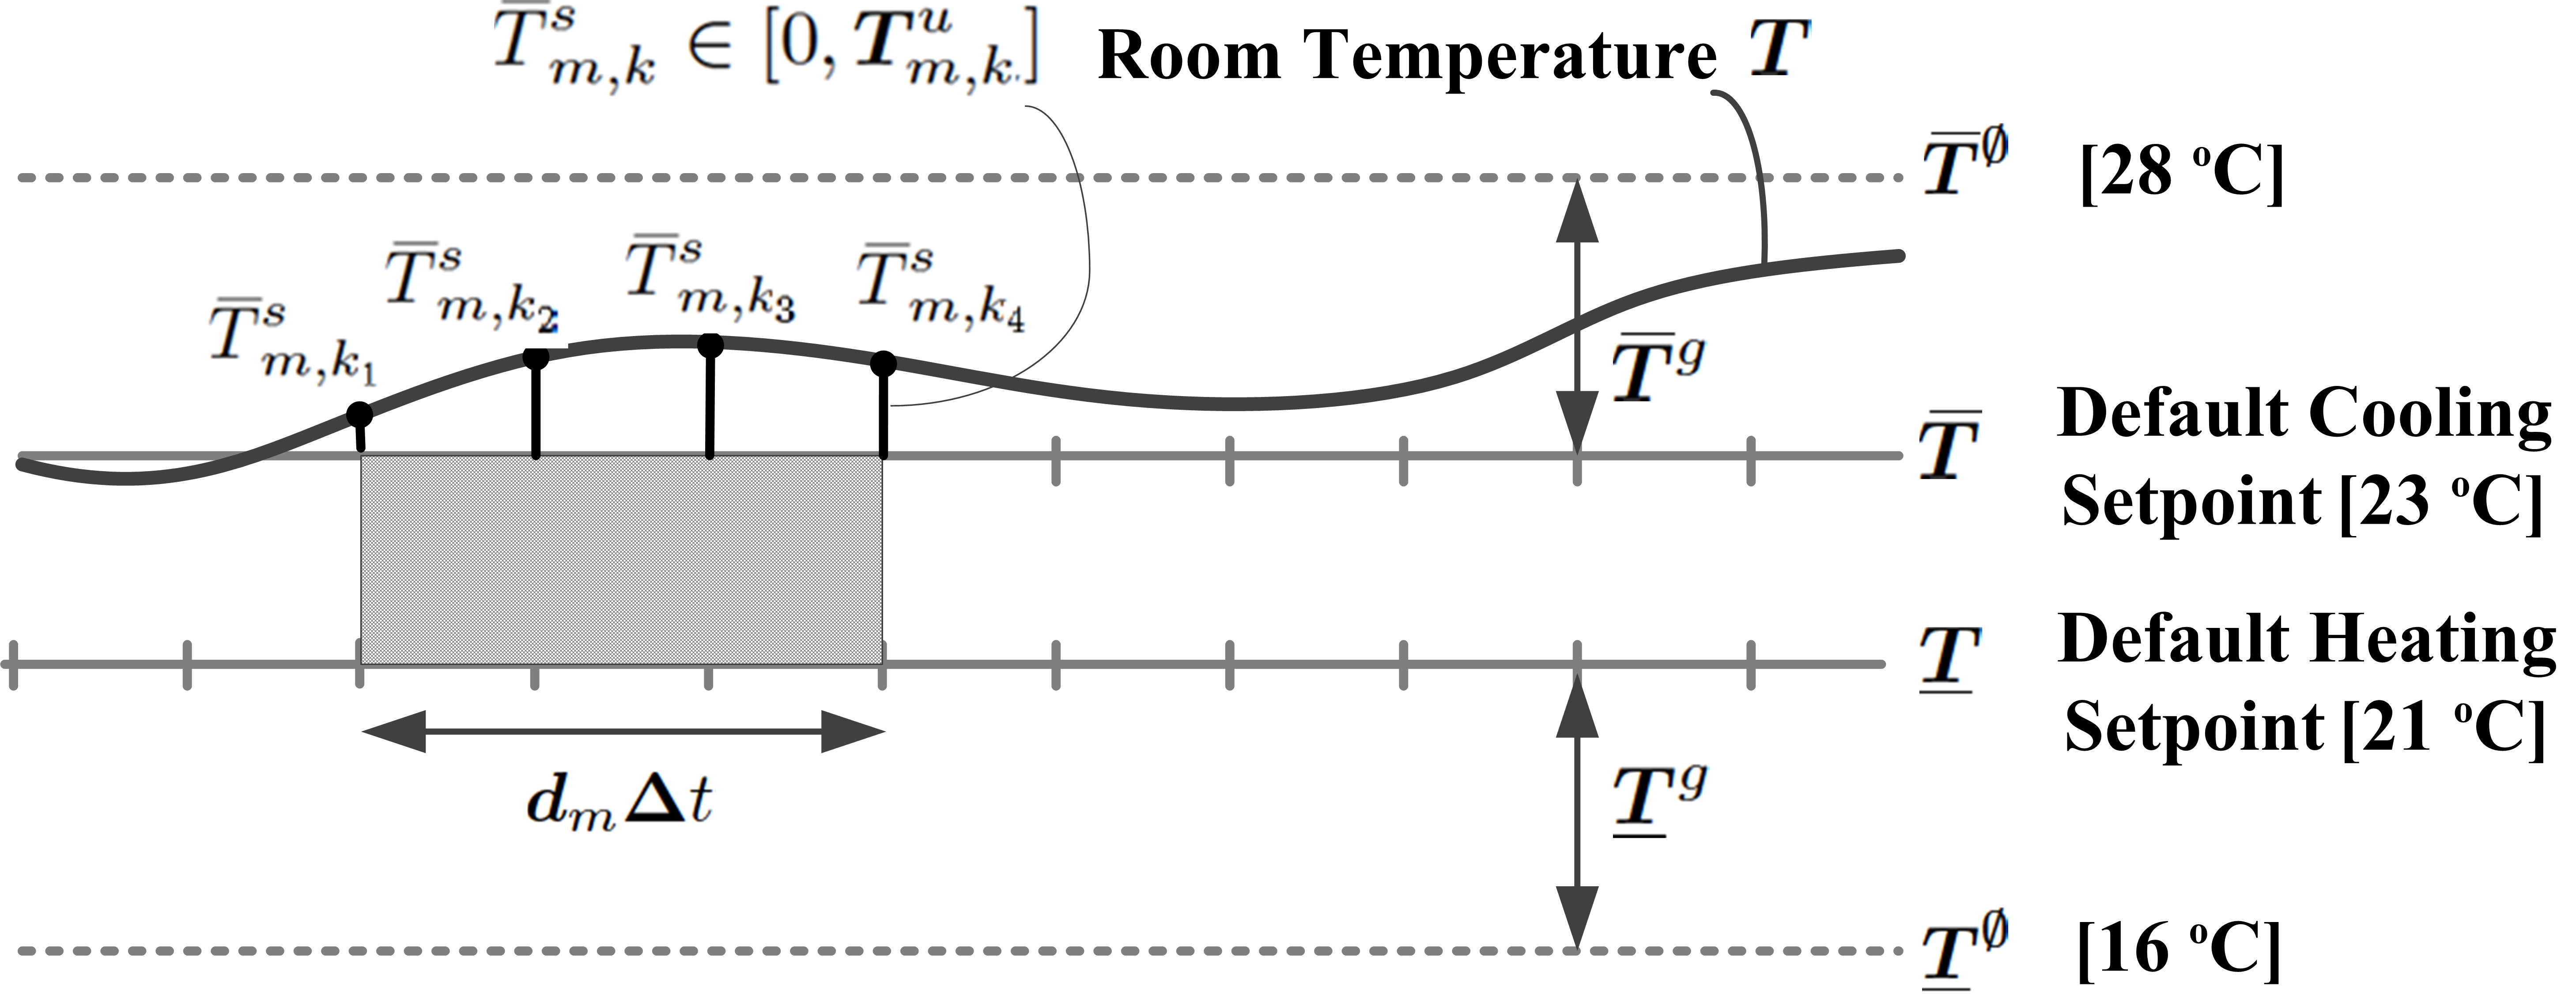
\includegraphics[height=1.6in,keepaspectratio]{figs/adaptivetemp.jpg}	
\caption{Adaptive temperature control}
\label{fig:adaptive}
\end{figure}

Fig.~\ref{fig:adaptive} illustrates the underlying concepts. In this example, activity $m$ occupies location $l$ for 3 times steps. Instead of keeping the room temperature between 21 to 23 celcius, the occupants are prepared to accept some temperature deviation from the default comfort bounds. The room temperature can deviate to $[\oversl{\bm T} + \oversl{T}^{s}]$ %, but is limited to $[\undersl{\bm T} - {\bm T}^u_m]$ 
at each time step $k$. However, the sum of $\oversl{T}^{s}$ over the 3 time steps must be kept below the cumulative temperature deviation allowed by the occupants. 

Let $m$ be a meeting scheduled to start at time step $j\in K_m$ in location $l$. To formalise these concepts, we introduce the following slack variables in the model $\undersl{T}^{s}_{m,k} \in [0, {\bm T}^u_{m,k}]$ and $\oversl{T}^{s}_{m,k} \in [0, {\bm T}^u_{m,k}]$, for $k\in K(i)$. ${\bm T}^u_{m,k}$ denotes the maximum allowable temperature deviation at time step $k$ of meeting $m$. These variables represent our unknown temperature violations above and below the default bounds $[\undersl{\bm{T}}, \oversl{\bm T}]$.
Based on these variables, the first guarantee we want to provide can be written as the adaptive counterpart of the fixed temperature bound constraints~\eqref{eq:atc_comfort}.
\begin{equation}\label{eq:rob:comfort}
\undersl{\bm{T}}^{\emptyset} + \undersl{\bm{T}}^{g}z_{l,k} - \undersl{T}^{s}_{m,k} \leq T_{l,k} \leq \oversl{\bm T}^{\emptyset} - \oversl{\bm{T}}^{g}z_{l,k} + \oversl{T}^{s}_{m,k}
\end{equation} 
%
The second guarantee is about bounding the cumulative temperature violation. First, we constrain the maximum cumulative temperature violation to a constant value $\bm{B}$. This can be formulated as follows,
\begin{equation}
\sum\limits_{k=j}^{j+{\bm d}_m -1}\left(\undersl{T}^{s}_{m,k}   +  \oversl{T}^{s}_{m,k} \right) \leq {\bm B} \label{eq:cum}
\end{equation}

We assume that $\bm{B}$ is certain, and can be derived based on the inputs from the occupants (refer to Section \ref{atc:mtd}) or from the outdoor temperature (refer to Section \ref{atc:oat}). To provide a probabilistic guarantee to the thermal comfort satisfaction, we implement a probabilistic version of Constraints \eqref{eq:cum}. We introduce random variables $\tilde{a}_{m,k}$, which represent the uncertainty over thermal comfort flexibility of the occupants, transforming these constraints into,
\begin{equation}
\sum\limits_{k=j}^{j+{\bm d}_m -1}\left(\undersl{T}^{s}_{m,k}   +  \oversl{T}^{s}_{m,k} + \tilde{a}_{m,k} \right) \leq {\bm B} \label{eq:cum_rand}
\end{equation}

\noindent The random variables $\tilde{a}_{m,k}$ reflect the uncertainty at each time step $k$ of meeting $m$, and take their values in the range $\left[\bar{a}_{m,k}-\hat{a}_{m,k}, \-\bar{a}_{m,k}+\hat{a}_{m,k}\right]$ uniformly and independently. These parameters are independent from the model variables, $\undersl{T}^{s}_{m,k}$ and $\oversl{T}^{s}_{m,k}$. Hence, we can consider additive functions \citep{hijazi2013robust}, in which the sum of all random variables $\tilde{a}_{m,k}$ corresponding to a meeting %  that is, $\sum\limits_{k=j}^{j+{\bm d}_m -1}{\tilde{a}_{m,k}}$ 
denotes the total disturbance to the constraint satisfaction.

Let $\tilde{a}_{m,k} = \bar{a}_{m,k} + \hat{a}_{m,k} \xi_{m,k}$, where $\xi_{m,k}$ are independent and uniformly distributed random variables in $\left[-1, 1\right]$. We re-write constraints \eqref{eq:cum_rand} to 

\begin{equation}
\sum\limits_{k=j}^{j+{\bm d}_m -1}\left(\undersl{T}^{s}_{m,k}   +  \oversl{T}^{s}_{m,k} + \bar{a}_{m,k} + \hat{a}_{m,k} \xi_{m,k}  \right)  \leq {\bm B} \label{eq:cum_rand_expand}
\end{equation}

We then resort to results from the Robust optimisation literature \citep{Elgh97,BenT98,BenT99,babonneau2009robust,hijazi2013robust} to be able to offer the following probabilistic guarantee,
\begin{equation}
\sc{Pr}\left(\sum\limits_{k=j}^{j+{\bm d}_m -1}\left(\undersl{T}^{s}_{m,k} + \oversl{T}^{s}_{m,k}  + \bar{a}_{m,k} + \hat{a}_{m,k} \xi_{m,k} \right)  \leq {\bm B} \right) \ge {\bm p}_m \label{eq:cum_bound_prob}
\end{equation}
where $\sc{Pr}\left(f_{\bm \xi}(x) \le 0\right)$ denotes the probability of satisfying constraint $f_{\bm \xi}(x) \le 0$ given the uncertainty created by the random vector $\xi_m$. In particular, based on \cite[Theorem 3.]{babonneau2009robust}, we can offer the above probabilistic guarantee by considering ellipsoidal uncertainty sets and enforcing the following constraint
 \begin{equation}\label{eq:radius}
 \sum\limits_{k=j}^{j+{\bm d}_m -1} {\xi}_{m,k}^2 \le \bm{\delta}_m^2,
 \end{equation}
where the the ellipsoid radius $\bm{\delta}_m$ is linked to the constraint satisfaction probability ${\bm p}_m$ as follows:
\begin{equation}
\label{eq:pm_delta_link}
\bm{p}_m \ge 1 - exp(-\bm{\delta}_m^2/1.5).
\end{equation}
For instance, a radius of $\bm{\delta}_m = 2.63$  leads to a constraint satisfaction probability $\bm{p}_m \ge 0.99$. 
Furthermore, based on \cite[Corollary 1.]{hijazi2013robust}, we can write the following deterministic equivalent of \eqref{eq:cum_bound_prob} without having to explicitly enforce \eqref{eq:radius},
\begin{equation}
\sum\limits_{k=j}^{j+{\bm d}_m -1}\left(\undersl{T}^{s}_{m,k}   +  \oversl{T}^{s}_{m,k} \right) + \sum\limits_{k=j}^{j+{\bm d}_m -1} \bar{a}_{m,k}  + \sum\limits_{i \in \mathcal{S}} \hat{a}_{m,i} + \sqrt{\left({\bm \delta}_m^2 - |\mathcal{S}|\right) \sum\limits_{i \notin \mathcal{S}} \hat{a}^2_{m,i}  } \leq {\bm B}
\label{eq:cum_bound_det}
\end{equation}

Constraints \eqref{eq:cum_bound_det} assure that the probability of temperature deviation being kept under its upper bound is always larger than ${\bm p}_m$. In other words, for any realization of the uncertain data $\tilde{a}_{m,k}$, these constraints impose the tightest right-hand side value, thus providing the highest protection (a.k.a upper bound) against uncertainty. This leads to a guarantee of constraint satisfaction given the probability ${\bm p}_m$. 

The set $\mathcal{S}$ is described in \cite[Proposition 1.]{hijazi2013robust}. 
For clarity, we repeat the procedure of generating set $\mathcal{S}$. 
%Let $\mathcal{S}$ be a set of indices defined as follow:
%
%\vspace{10pt}
%$\forall \hat{a}_m \in \left(\mathbb{R}^\ast\right)^{d_m}, \delta \in [0, \sqrt{d_m}]: \exists \mathcal{S}\subset\left\{1, 2, \ldots,d_m\right\} \textsl{s.t.}
%\left\{
%\begin{array}{lll}
%\!|\mathcal{S}| \leq \delta^2 \\
%\!\frac{\sqrt{\delta_2 - |\mathcal{S}|}|\hat{a}_{m,i}|}{\sqrt{\sum\limits_{i \notin \mathcal{S}}\hat{a}^2_{m,i}}} > 1, \forall i \in \mathcal{S} \\
%\!\frac{\sqrt{\delta_2 - |\mathcal{S}|}|\hat{a}_{m,i}|}{\sqrt{\sum\limits_{i \notin \mathcal{S}}\hat{a}^2_{m,i}}} \leq 1, \forall i \notin \mathcal{S} \\
%\end{array}
%\right.$
%\vspace{10pt}
Assume the elements of vector $\hat{a}$ are sorted in descending order of their absolute values, i.e. $|\hat{a}_{m,i}| \geq \left|\hat{a}_{m,i+1}\right|, \forall i \in \left\{j, j+1, \ldots, j+d_m-1\right\}$ and consider the following procedure:

\vspace{10pt}
\begin{algorithm}[H]
\KwData{$\hat{a}_m; \mathcal{S} := \emptyset; k := 1;$}
\While{$k < n-1$}{
\eIf{$ \frac{\sqrt{\delta^2-\left|S\right|}\left|\hat{a}_{m,k}\right|}{\sqrt{\sum_{i \geq k}{\hat{a}_{m,i}^2}}} \leq 1$}{\Return $\mathcal{S}$}
{$\mathcal{S} := \mathcal{S}\cup{k}; k := k+1;$}
}
\Return {$\mathcal{S}$}
\end{algorithm}
\vspace{10pt}




%--------------------------------------
Since activity locations and start times are not known in advance, we introduce variables $\undersl{T}^{\xi}_{l,k}$ (resp. $\oversl{T}^{\xi}_{l,k}$) such that $\undersl{T}^{\xi}_{l,k} = \undersl{T}^{s}_{m,k}$ and $\oversl{T}^{\xi}_{l,k} = \oversl{T}^{s}_{m,k}$ when activity $m\in M$ occupies location $l\in L$ at time slot $k \in K$, i.e., when $y_{m,l,k} = 1$.

For online scheduling, in order to accommodate activities that span multiple scheduling horizons, we also introduce the inputs ${\bm T}^{prev}_{m} = \mathop{\sum \limits_{k \in K: k< k(i)}} (\undersl{\bm T}^s_{m,k} + \oversl{\bm T}^s_{m,k})$, which accounts for the amount of cumulative violation consumed before the start of the current session. Recall also from Section~\ref{sec:online:sche_model} that meetings that have been scheduled in previous sessions have their start time set ${\bm K}_m$, location set ${\bm  L}_m$ and duration ${\bm d}_m$ reduced accordingly when the current session starts. 

With these notations, the overall adaptive temperature control constraints replacing the fixed temperature constraints~\eqref{eq:atc_comfort} in the HVAC control model are the following.
\begingroup
\begin{align}
&\undersl{\bm{T}}^{\emptyset} + \undersl{\bm{T}}^{g}z_{l,k} - \undersl{T}^{\xi}_{l,k} \leq T_{l,k} \leq \oversl{\bm T}^{\emptyset} - \oversl{\bm{T}}^{g}z_{l,k} + \oversl{T}^{\xi}_{l,k}\quad \forall l \in L, k \in K(i) \label{eq:ad:comfort}\\ 
&\undersl{T}^{s}_{m,k} - \hat{{\bm T}}\left(1 - y_{m,l,k}\right) \le \undersl{T}^{\xi}_{l,k}  \leq  \undersl{T}^{s}_{m,k} +\hat{{\bm T}} \left(1 - y_{m,l,k}\right) ~ \forall m \in M, l \in L, k \in K(i) \label{eq:xi_lb_leq}  \\
& \oversl{T}^{s}_{m,k} - \hat{{\bm T}}\left(1 - y_{m,l,k}\right) \le \oversl{T}^{\xi}_{l,k} \leq   \oversl{T}^{s}_{m,k} + \hat{{\bm T}}\left(1 - y_{m,l,k}\right) ~ \forall m \in M, l \in L, k \in K(i) \label{eq:xi_ub_leq}
\end{align}

Constraints~\eqref{eq:ad:comfort}\ are the adaptive bound constraints.
Constraints~(\ref{eq:xi_lb_leq}-\ref{eq:xi_ub_leq}) are the on-off constraints defining the variables $\undersl{T}^{\xi}_{l,k}$ and $\oversl{T}^{\xi}_{l,k}$ with $\hat{{\bm T}} = \max\limits_{m \in M, k \in K_m}\{{\bm T}^u_{m,k}\}$.  %$\hat{{\bm T}} = \max\limits_{m \in M}\{{\bm T}^u_m\}$. 


\section{Cumulative Temperature Violation}

The challenge we face here is \textsl{how to determine the cumulative temperature violation}. In the following section, we present two methods that define this input from different perspectives. 


\subsection{Maximum Temperature Deviation Aware (MTDA) Approach} \label{atc:mtd}

In the \emph{\textsl{maximum temperature deviation aware}} approach, we allow the occupants to indicate their level of tolerance to temperature fluctuation in the form of [high, medium, low] comfort tolerance level. Given these inputs, we then derive the following parameters to calculate the cumulative temperature violation during the occupied periods:
\begin{enumerate}	
	\item the maximum temperature deviation allowed at any time, 
	\item the duration for which the occupant would be willing to let the temperature deviate from the standard cooling and heating setpoints, and
	\item a probability threshold indicating the level of robustness in terms of thermal comfort guarantee.
\end{enumerate}
From an implementation point-of-view, the parameters that are linked to each comfort tolerance level can either be made known to the users or kept hidden. In either way, these parameters can be tuned periodically based on different operational conditions such as changes in outdoor temperature, building load and/or occupants' perceptions on thermal comfortness.

In this method, the maximum temperature deviation allowed and the maximum duration for which the occupant is willing to set a higher (resp. lower) cooling (resp. heating) setpoints are pre-defined. We denote this approach as \emph{\textsl{maximum temperature deviation aware}} as this method allows the occupants to anticipate the maximum temperature deviation they would experience throughout the activity period. In other words, the occupants explicitly decide the highest temperature violation allowed during the activity through input parameters. However, it does not consider outdoor temperature. 

%The first method is \textsl{maximum temperature deviation aware}, where occupants explicitly decide the highest temperature violation allowed during the activity through input parameters.
%In this approach, we calculate the cumulative temperature violation based on the occupants' inputs. 
Specifically, the input parameters we consider for a meeting request $m$ are $F_m=\langle \bm{T^u_m}, \bm{\alpha_m}, \bm{p_m}\rangle$. 
With these inputs, the HVAC control will guarantee: a) that the zone temperature will never exceed $[\undersl{\bm T} - \bm{T^u_m}, \oversl{\bm T}+\bm{T^u_m}]$ at any point during the activity, that is $\bm{T^u_{m,k}}$ is equivalent to $\bm{T^u_m}$ for all time step $k$ throughout the activity period, b) that the maximum cumulative temperature deviation ${\bm B} = \bm{\alpha_m} \bm{T^u_m} $, that is ${\bm B}$ is equivalent to the maximum duration $\bm{\alpha_m}$ during which the occupants would be willing to accept the maximum temperature duration $\bm{T^u_m}$, and c) that with probability at least $\bm{p_m}$, the thermal comfort of the occupants should be protected.
To achieve this, we re-write constraints \eqref{eq:cum_bound_det} to 
\begin{equation}
\begin{split}
\sum\limits_{k=j}^{j+\bm{d_m} -1}\left(\undersl{T}^{s}_{m,k} + \oversl{T}^{s}_{m,k} \right) 
& + \sum\limits_{k=j}^{j+\bm{d_m} -1} \bar{a}_{m,k} + \sum\limits_{i \in \mathcal{S}} \hat{a}_{m,i} + \sqrt{\left(\bm{\delta_m^2} - |\mathcal{S}|\right) \sum\limits_{i \notin \mathcal{S}} \hat{a}^2_{m,i}} \\
& \leq \frac{\bm{\alpha_m} \bm{T^u_m}}{\bm{\Delta_t}} - \bm{T^{prev}_m} \quad  \forall m \in M(i), j \in K_m 
%\sum\limits_{k=j}^{j+\bm{d_m}-1} \left(\undersl{T}^{s}_{m,k} + \oversl{T}^{s}_{m,k} \right) + \sum\limits_{k=j}^{j+\bm{d_m}-1} \bar{a}_{m,k} &+ \sum\limits_{i \in \mathcal{S}} \hat{a}_{m,i} + \sqrt{\left(\bm{\delta_m^2} - |\mathcal{S}|\right) \sum\limits_{i \notin \mathcal{S}} \hat{a}^2_{m,i}  }  \\ 
%& \leq \frac{\bm{\alpha_m} \bm{T^u_m}}\bm{\Delta_t} - \bm{T^{prev}_m} \quad  \forall m \in M(i), j \in K_m 
\end{split}
\label{eq:cum_bound_det_mtd}
\end{equation}

The random variables $\tilde{a}_{m,k}$ which reflect the uncertainty of thermal comfort at time step $k$ of meeting $m$ have a value within $\left[\bar{a}_{m,k}\!-\!\hat{a}_{m,k}, \bar{a}_{m,k}\!+\!\hat{a}_{m,k}\right]$. 
For simplicity, the nominal factor $\bar{a}_{m,k}$ is set to 0, and $\hat{a}_{m,k}$ is 0.5.
$\bm{\delta_m}$ is pre-calculated based on Equations \eqref{eq:cum_bound_prob}-\eqref{eq:pm_delta_link}. For instance, a constraint satisfaction probability of $p_m = [0.99, 0.75, 0.5]$ is equivalent to $\bm{\delta_m} = [2.63, 1.41, 1]$

Constraints~\eqref{eq:slack_lb_x} and ~\eqref{eq:slack_ub_x} bound the maximum temperature deviation to ${\bm T}^u_m$ when a location is occupied and force the corresponding slack to zero when a location is unoccupied. 
\begingroup
\begin{align}
&\undersl{T}^{\xi}_{l,k}  \leq \sum\limits_{m \in M(i)}\bm{T^u_m} y_{m,l,k} \quad  \forall l \in L, k \in K(i) \label{eq:slack_lb_x}  \\
&\oversl{T}^{\xi}_{l,k}   \leq \sum\limits_{m \in M(i)}\bm{T^u_m} y_{m,l,k} \quad  \forall l \in L, k \in K (i) \label{eq:slack_ub_x}
\end{align}

The overall adaptive temperature constraints using this approach is simply obtained by replacing the fixed temperature constraint \eqref{eq:atc_comfort} with equations \eqref{eq:ad:comfort}-\eqref{eq:slack_ub_x} in the HVAC control model.



\subsection{Outdoor Temperature Aware (OATA) Approach} \label{atc:oat}

In the \emph{\textsl{outdoor temperature aware}} approach, we use outdoor weather forecast to derive the maximum cumulative temperature violation ${\bm B}$. Similar to the MTDA approach, the occupants shall indicate their level of tolerance to temperature fluctuation in the form of [high, medium, low] comfort tolerance level. Given these inputs, we then calculate the cumulative temperature violation during the occupied periods using:
\begin{enumerate}
	\item the duration and time windows for which the activity can be scheduled, 
	\item the temperature gap between the forecast outdoor temperature and the standard cooling/heating setpoints within the time windows, and
	\item a probability threshold indicating the level of robustness in terms of thermal comfort guarantee.
\end{enumerate}
This method is \emph{\textsl{outdoor temperature aware}} as it considers the findings of \cite{de1998developing} which indicate that the occupants' thermal acceptability and comfort are correlated to the outdoor temperature. In this method, the maximum temperature deviation is adjusted according to the outdoor temperature. %It automatically obtains the maximum cumulative temperature deviation allowed based on the outdoor temperature.

%The second method is \textsl{outdoor temperature aware}, where outdoor weather forecast is used to derive the cumulative temperature violation. 
%In this approach, we calculate the cumulative temperature violation based on outdoor weather forecast. 
The input parameters we consider for a meeting request $m$ are $F_m=\langle \bm{d_m},\bm{K_m}, \bm{p_m}\rangle$. $\bm{d_m}$ denotes the duration of activity, $\bm{K_m}$ consists of all possible start time slots for meeting $m$ and $\bm{p_m}$ denotes the probability of constraint satisfaction guarantee towards the occupants' thermal comfort.
We identify the temperature gap $g_{m,k}$ between the forecast outdoor temperature and the standard cooling/heating setpoints for each time step $k$ within the scheduling time window of activity $m$ as follows:

\vspace{10pt}
$g_{m,k} = 
\left\{
\begin{array}{lll}
\!(\bm{T^{OA}_k} - \oversl{T} + \bm{c}) & \mbox{for $\bm{T^{OA}_k} > \oversl{T}$}\\
\!(\undersl{T} - \bm{T^{OA}_k} - \bm{c}) & \mbox{for $\undersl{T} > \bm{T^{OA}_k}$}\\
\!\bm{c} & \mbox{for $\undersl{T} \leq \bm{T^{OA}_k} \leq \oversl{T}$}\\
\end{array}
\right.$
\vspace{10pt}

$c$ denotes the minimum allowable temperature deviation at each time step. We then re-write constraints \eqref{eq:cum_bound_det} to 
%based on the sum of these temperature gap normalized to the duration of the activity over the number of possible scheduling slots. To achieve this, we re-write constraints \eqref{eq:cum_bound_det} to 
\begin{equation}
\begin{split}
%\sum\limits_{k=j}^{j+{\bm d}_m -1}\left(\undersl{T}^{s}_{m,k} \!+\! \oversl{T}^{s}_{m,k} \right) \!+\! \sum\limits_{k=j}^{j+{\bm d}_m -1} \bar{a}_{m,k} \!+\! \sum\limits_{i \in \mathcal{S}} \hat{a}_{m,i} \!+\! \sqrt{\left({\bm \delta}_m^2 - |\mathcal{S}|\right) \sum\limits_{i \notin \mathcal{S}} \hat{a}^2_{m,i}}\!\leq \!\sum\limits_{k=j}^{j+{\bm d}_m -1}\!\!g_{m,k}\!\times\!\frac{\bm d_m}{\left|K_m\right|+d_m}\!-\!{\bm T}^{prev}_{m} 
\sum\limits_{k=j}^{j+\bm{d_m} -1}\left(\undersl{T}^{s}_{m,k} + \oversl{T}^{s}_{m,k} \right) 
& + \sum\limits_{k=j}^{j+\bm{d_m} -1} \bar{a}_{m,k} + \sum\limits_{i \in \mathcal{S}} \hat{a}_{m,i} + \sqrt{\left(\bm{\delta_m^2} - |\mathcal{S}|\right) \sum\limits_{i \notin \mathcal{S}} \hat{a}^2_{m,i}} \\
& \leq \sum\limits_{k=inf(K_m)}^{sup(K_m)+\bm{d_m}-1} g_{m,k} \times \frac{\bm{d_m}}{\left|K_m\right|+\bm{d_m-1}} - \bm{T^{prev}_{m}}  \quad  \forall m \in M(i), j \in K_m
\end{split}
\label{eq:cum_bound_det_oat}
\end{equation}

The random variables $\tilde{a}_{m,k}$ which reflect the uncertainty over thermal comfort flexibility at time step $k$ of meeting $m$ has a value within $\left[\bar{a}_{m,k}\!-\!\hat{a}_{m,k}, \bar{a}_{m,k}\!+\!\hat{a}_{m,k}\right]$. The nominal factor $\bar{a}_{m,k}$ is set to 0, and $\hat{a}_{m,k}$ is equivalent to $g_{m,k}$. ${\bm \delta}_m$ is pre-calculated based on Equations \eqref{eq:cum_bound_prob}-\eqref{eq:pm_delta_link}. Note that $\sum\limits_{k=inf(K_m)}^{sup(K_m)+{\bm d}_m -1}g_{m,k}$ denotes the sum of temperature gaps throughout all possible scheduling slots of activity $m$. This implies that an activity with a flexible scheduling window (i.e. a large number of possible scheduling slots) would allow large cumulative temperature violation. 
However, as a complement to the scheduling flexibility given, this is avoided by normalising the constraints using the number of possible start time slots, $bm{\left|K_m\right|}$.
%However, as a compliment to the scheduling flexibility given, constraints \eqref{eq:cum_bound_det_oat} normalize it with the duration of the activity over the number of possible scheduling slots allowed. This means that, for two activities with similar duration $\bm{d_m}$, the activity with more flexibility on scheduling time window is prone to have a relatively lower cumulative temperature violation compares to the activity with lesser flexibility on scheduling time window.

In this approach, the maximum temperature deviation at each time step $k$ of a meeting $m$ is outdoor weather dependent. 
Constraints~\eqref{eq:oata_slack_lb_x} and ~\eqref{eq:oata_slack_ub_x} bound the maximum temperature deviation to ${\bm T}^u_{m,k}$ when a location is occupied and force the corresponding slack to zero when a location is unoccupied. Specifically, ${\bm T}^u_{m,k}$ is the difference between outdoor temperature and the setpoints. However, to assure that the comfort deviation is within a reasonable bound, we limit the temperature gap to an interval of $\left[0.5, 3.0\right]^{\circ}\mathrm{C}$. 

\begingroup
\begin{align}
&\undersl{T}^{\xi}_{l,k}  \leq \sum\limits_{m \in M}{\bm T}^u_{m,k} y_{m,l,k} \quad  \forall l \in L, k \in K \label{eq:oata_slack_lb_x}  \\
&\oversl{T}^{\xi}_{l,k}   \leq \sum\limits_{m \in M}{\bm T}^u_{m,k} y_{m,l,k} \quad  \forall l \in L, k \in K \label{eq:oata_slack_ub_x}
\end{align}
\endgroup

The overall adaptive temperature constraints using this approach is simply obtained by replacing the fixed temperature constraint \eqref{eq:atc_comfort} with equations \eqref{eq:ad:comfort}-\eqref{eq:xi_ub_leq} and \eqref{eq:cum_bound_det_oat}-\eqref{eq:oata_slack_ub_x} in the HVAC control model.


\section{Experiments} \label{sec:atc_exp}

We implement our MTDA-based and OATA-based adaptive temperature control approaches on the online model in Chapter \ref{cha:online}. To examine the effectiveness of these flexible temperature control approaches, we conduct empirical studies using the same buildings and meetings datasets for fixed temperature control. % in chapter \ref{cha:online} as well. 
These datasets are grouped into \textsl{x} number of activities (M) and \textsl{y} locations (R): [10M-4R, 20M-20R, 50M-20R, 100M-20R, 200M-20R, 50M-50R, 100M-50R, 200M-50R, 500M-50R]. 
The instances within each dataset contain varying settings of time flexibility $\left|K_m\right| \in \left\{1,2,4,8,32\right\}$ and request-to-start time $\left\{\mbox{10 minutes, 1 hour, 4 hours, 24 hours}\right\}$.
% similar to the datasets used in fixed setpoints control approach, but 
We then configure these instances with different temperature flexibility as follows.
% We define different flexibility settings that indicates the level of tolerance for the room temperature deviation from the standard heating (21$^{\circ}\mathrm{C}$) and cooling (23$^{\circ}\mathrm{C}$) setpoints. 

For the MTDA approach, 7 settings of $F_m=\langle {\bm T}^{u}_m, {\bm \alpha}_m, {\bm p}_m\rangle$ are defined based on the maximum temperature deviation (D) allowed and the expected level of thermal comfort guarantee (G):
\begin{itemize}	
	\item High Deviation, High Robustness (HDHG) : $F_m=\left\langle 2.5, 40, 0.75\right\rangle$,
	\item High Deviation, Medium Robustness (HDMG) : $F_m=\left\langle 2.5, 40, 0.50\right\rangle$,
	\item High Deviation, Low Robustness (HDLG) : $F_m=\left\langle 2.5, 40, 0\right\rangle$,
	\item Medium Deviation, High Robustness (MDHG) : $F_m=\left\langle 1.5, 35, 0.75\right\rangle$,
	\item Medium Deviation, Medium Robustness (MDMG) : $F_m=\left\langle 1.5, 35, 0.50\right\rangle$,
	\item Medium Deviation, Low Robustness (MDLG) : $F_m=\left\langle 1.5, 35, 0\right\rangle$, and
	\item Low Deviation, Low Robustness (LDLG) : $F_m=\left\langle 0.5, 30, 0\right\rangle$.	
\end{itemize}
Note that we omit the settings for high and medium level thermal comfort guarantee for \textsl{Low Deviation} as the temperature violation allowed is already very low. Each dataset contains 560 problem instances, giving a total of 5040 instances for the MTDA approach.

For OATA approach, we define 3 settings that vary on the thermal comfort guarantee, i.e. ${\bm p}_m = 0.75 \mbox{ (HG)}, 0.5 \mbox{ (MG)}, 0 \mbox{ (LG)}$. The temperature deviation for each instance is dependent on the outdoor temperature, the meeting duration $\bm{d_m}$, and the possible start time slots $\bm{K_m}$. We set $c$=0.5. Each dataset contains 240 problem instances, giving a total of 2160 instances for the OATA approach. %obtained with the following configurations.
All our experiments were run on a cluster consisting of a 2 $\times$ AMD 6-Core Opteron 4334, 3.1GHz with 64GB memory using \cite{gurobi} solver version 6.5.


\subsection{Impacts of Adaptive Temperature Control} \label{sec:atc_impacts}

\begin{figure}
\centering
\begin{tabular}{c}
  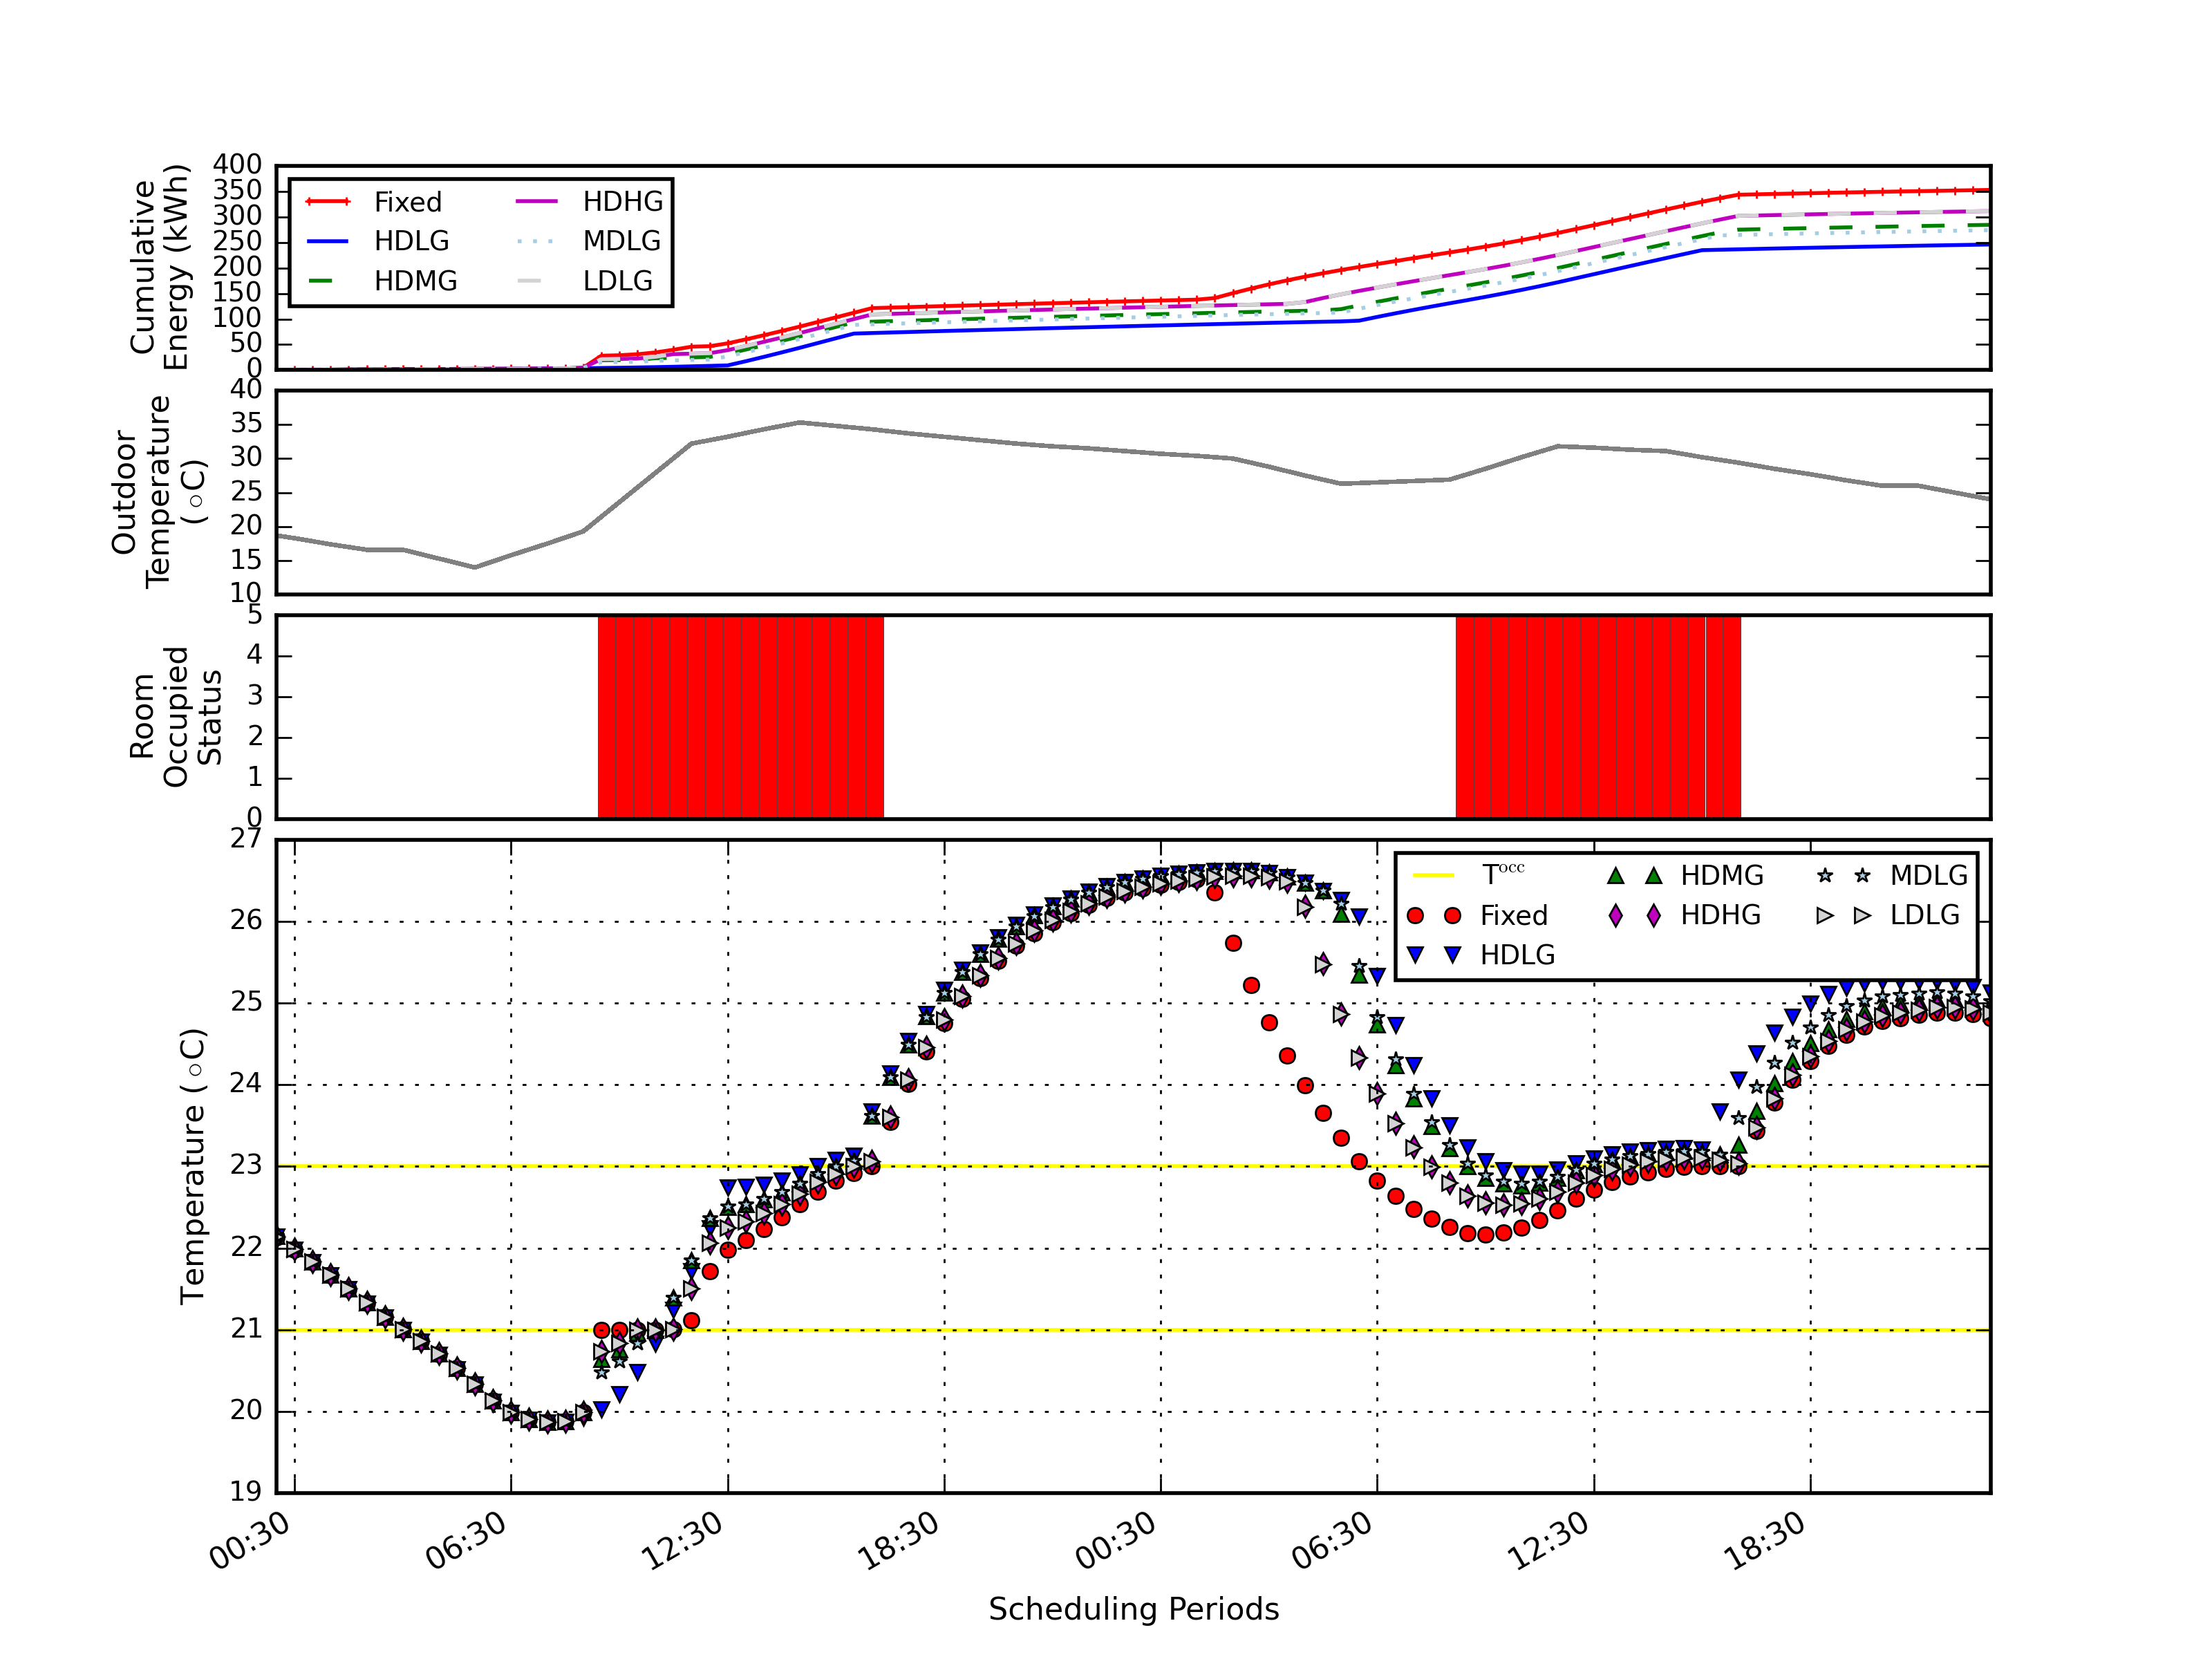
\includegraphics[width=1\linewidth]{figs/atc_mtda.png} \\
(a) Maximum temperature deviation aware approach \\[6pt]
  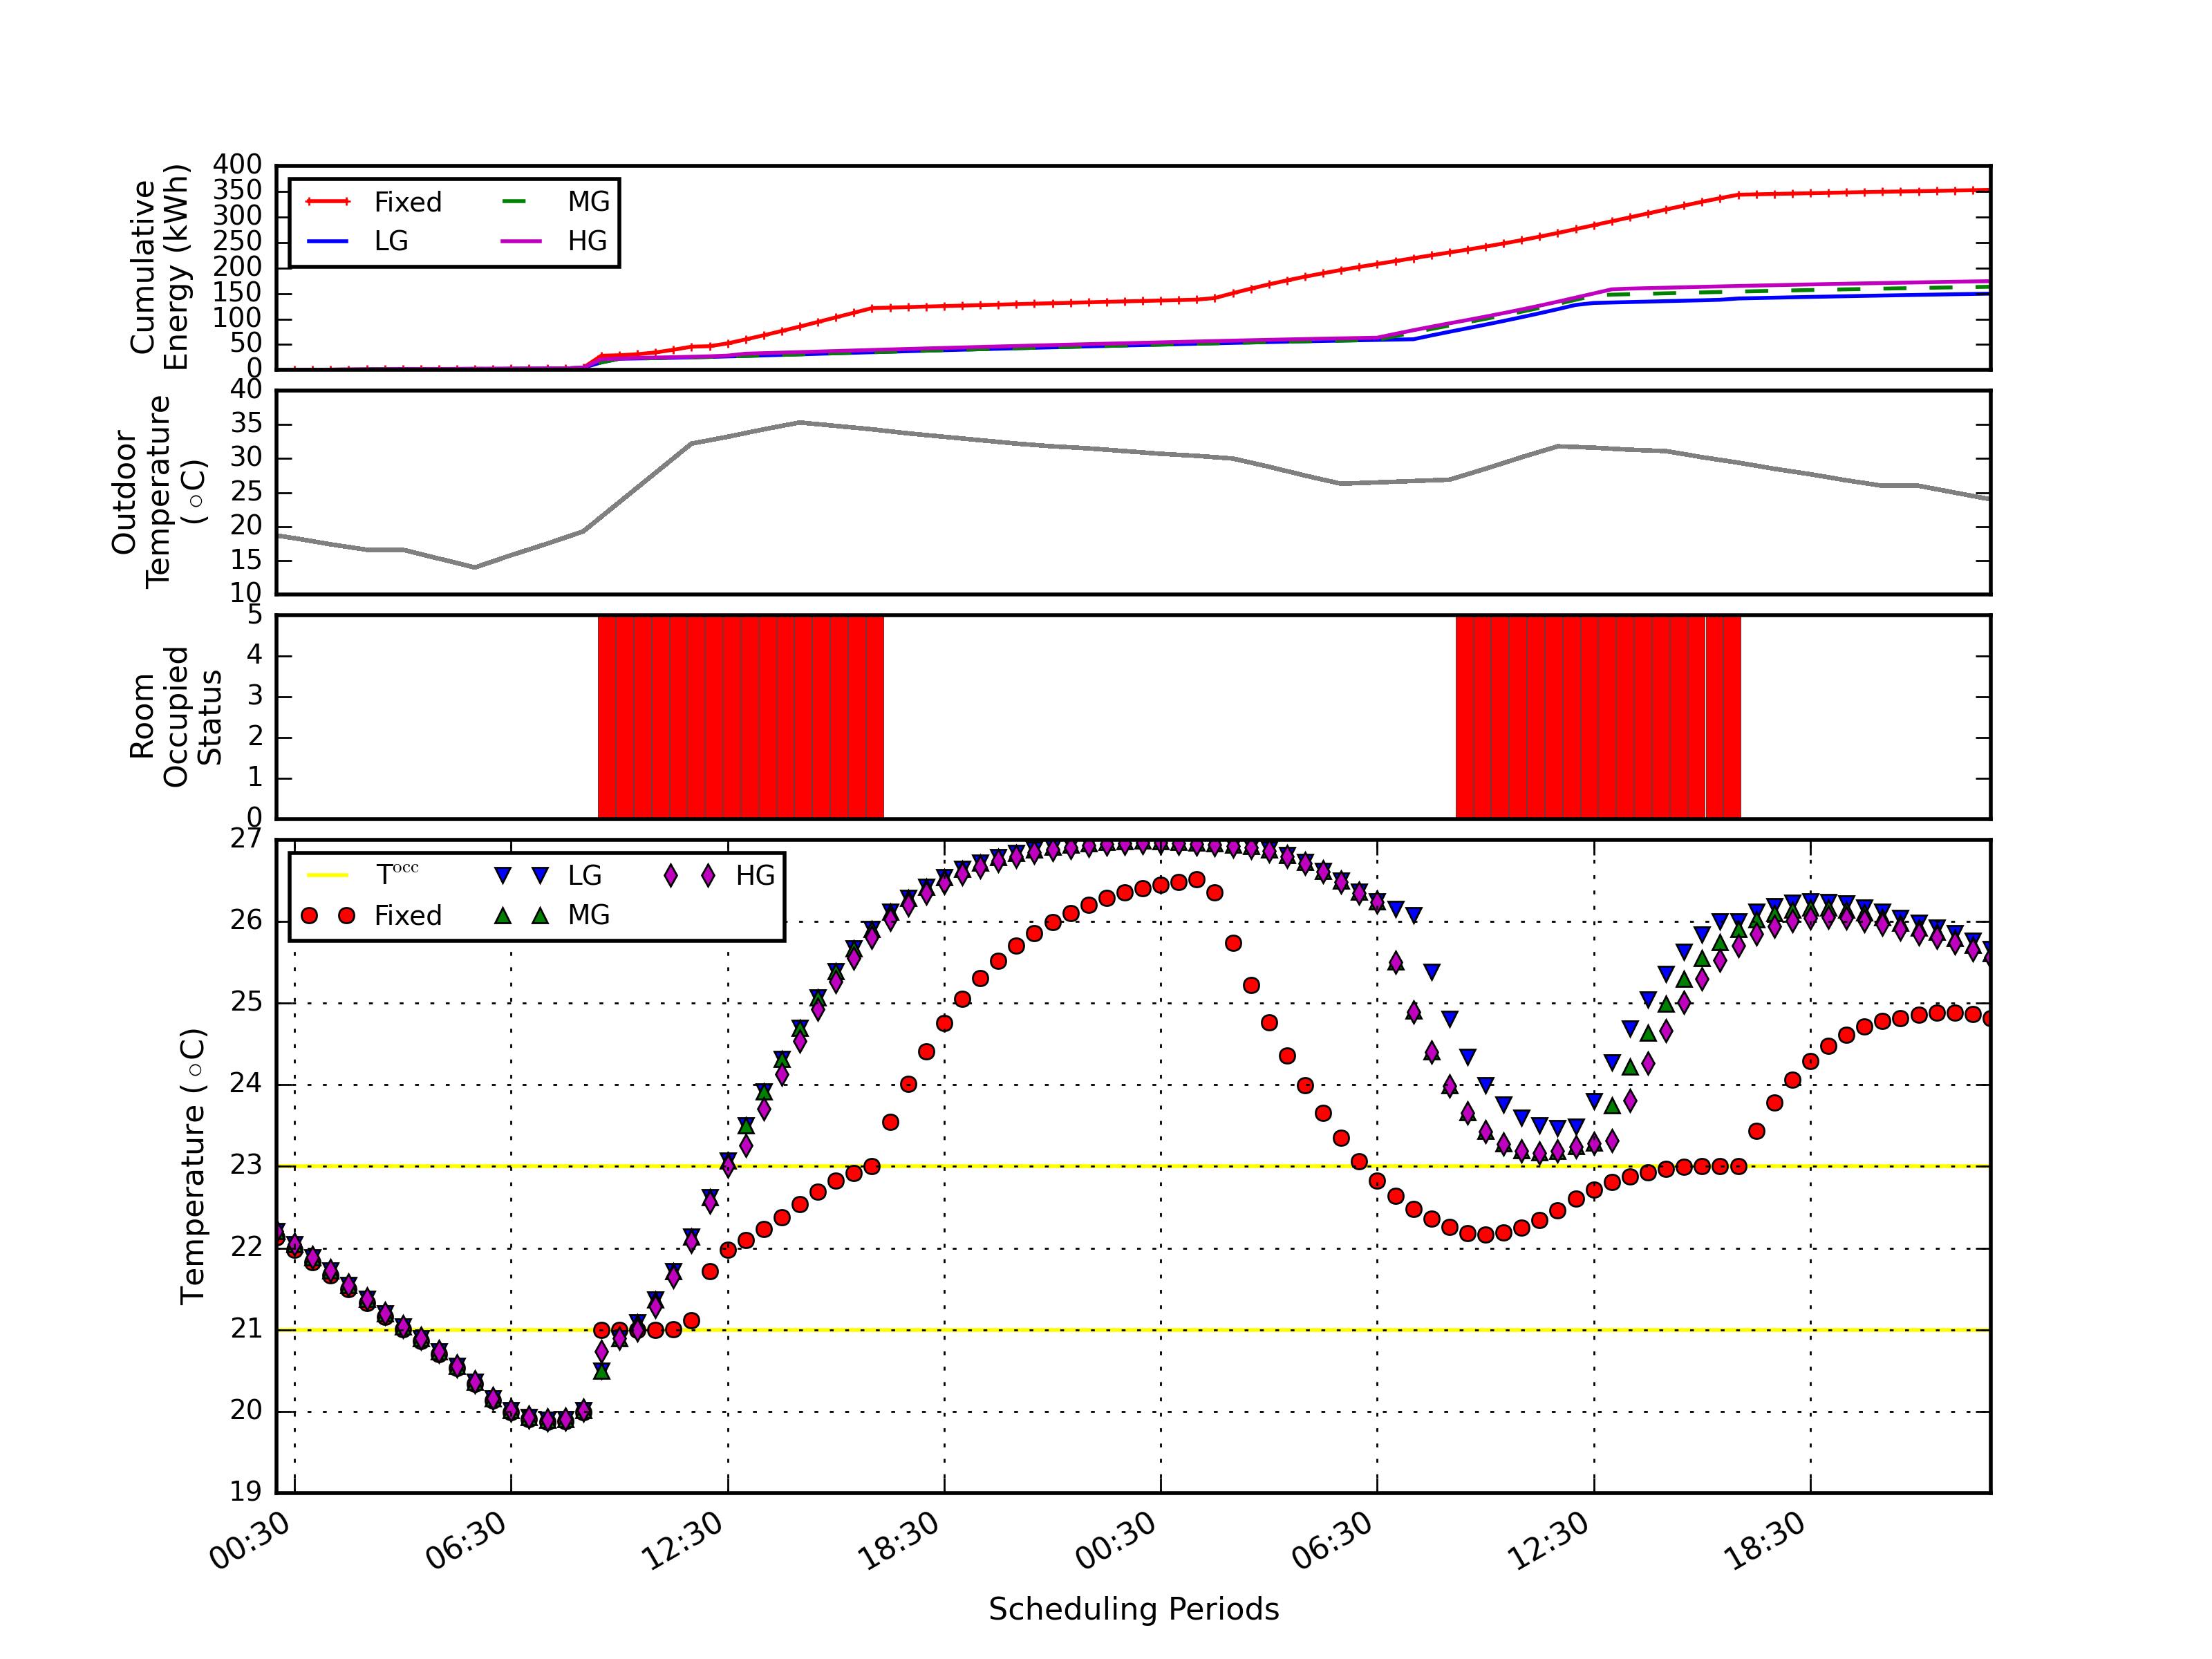
\includegraphics[width=1\linewidth]{figs/atc_oata.png} \\
(b) Outdoor temperature aware approach \\[6pt]
\end{tabular}
\caption{Solution examples}
\label{fig:atc_impacteg}
\end{figure}

We start by examining the impact of adaptive temperature control on energy savings and occupants' thermal comfort. In the conventional approach, the temperature setpoints are configured within a fixed bound. Our adaptive temperature control approaches adjust the temperature setpoints based on the occupants' thermal comfort flexibility. Figure \ref{fig:atc_impacteg} compares the occupied room temperatures using MTDA and OATA approaches. For this experiment, a room is being occupied from 09:00 to 17:00 for 2 days. 

Observe that in Figure \ref{fig:atc_impacteg}(a), the room temperature is kept within the maximum temperature deviation allowed when the HVAC is running with the MTDA approach. For the fixed temperature approach, the occupied room temperature is always within 21$^{\circ}C$ to 23$^{\circ}C$. Whilst the deviation of occupied room temperature from the standard setpoints will never exceed 0.5$^{\circ}C$ for LDLG approach, 1.5$^{\circ}C$ for MDLG  approach and 2.5$^{\circ}C$ for HDLG, HDMG and HDHG approaches. 
%445.750583427
%312.44219608
%364.233705337
%398.3531414
%350.886041277
%398.441687509
The experiment shows that with a small deviation from the fixed temperature setpoints, the HDLG approach generates a 30\% (133 kWh) of energy savings compared to the conventional approach. With better thermal comfort guarantees, the HDHG and LDLG approaches still lead to about 10\% (47 kWh) of energy savings. 
Note that to improve readability, the MDMG and MDLG are omitted in this figure. %the MTDA approach.

Figure \ref{fig:atc_impacteg}(b) illustrates the results of adaptive temperature control using OATA approach. Observe that the room temperature fluctuates according to the outdoor temperature, with a deviation up to 3$^{\circ}\mathrm{C}$ (i.e. 26$^{\circ}\mathrm{C}$) during occupied. Following the findings of \cite{de1998developing}, the HVAC operates in such as a way that the room temperature is slightly higher in a hotter day, and slightly lower in a cooler day. This leads to only half of the energy consumption required by the conventional fixed temperature setpoints control, which brings significant energy savings. Observe that the  LG and HG approaches have a difference of 0.3$^{\circ}\mathrm{C}$ to 1$^{\circ}\mathrm{C}$ in terms of room temperature, with varying level of thermal comfort guarantee. Thus, whilst the OATA approach sets the maximum cumulative temperature violation according to the outdoor temperature, it also offers some kind of comfort guarantee to the occupants with a configurable parameter.


\subsection{Energy Savings of Adaptive Temperature Control} \label{sec:atc_energy}

Next we examine the benefits of our adaptive temperature control in terms of energy savings. Because HVAC consumption is highly dependent on the occupied temperature setpoint, we show that even a small variation from the original setpoints can lead to large energy savings.

Figure \ref{fig:atc_eg} shows the energy savings obtained with MTDA-based and OATA-based adaptive temperature control as a percentage of the fixed temperature control consumption. Considering the MTDA-based approach with least comfort guarantee (LG), it achieves up to [5.7\%, 12.5\%, 16.04\%] depending on the [low (LDLG), medium (MDLG), high (HDLG)] temperature deviation allowed by the occupants. The OATA-based approach shows a savings up to [10.1\%, 13.05\%, 14.4\%] for [low (LG), medium (MG), high (HG)] settings. 

%Observe that the temperature flexibility settings have obvious energy savings impact on the MTDA approach in Figure \ref{fig:atc_eg}(a) than the OATA approach in Figure \ref{fig:atc_eg}(b). 
If we compare Figure \ref{fig:atc_eg}(a) with Figure \ref{fig:atc_eg}(b), we notice that in terms of energy savings, the MTDA approach is impacted by the temperature flexibility more than the OATA approach. 
This is due to the cumulative temperature deviation in the MTDA approach being bounded by the maximum temperature deviation allowed for each flexibility setting. The LDLG configuration with a maximum deviation of 0.5$^\circ$C over a period of 30 minutes imposes tighter constraints than that of the HDLG setting with a maximum of 2.5$^\circ$C over 40 minutes. This results in a difference of energy savings of about 5\% on average.

In contrast, for the OATA approach, the cumulative deviation is bounded by the outdoor temperature, which is similar for all settings. Thus the difference of energy savings amongst various thermal comfort guarantee levels for this approach is merely 2\% on average. A similar trend is also shown in Figure \ref{fig:atc_memr} and Figure \ref{fig:atc_mehr}, where the energy savings of the MTDA approach with the same maximum temperature deviation but different level of thermal comfort guarantee are depicted. 

From our observations, ensuring thermal comfort comes at a price. Having less constrained temperature violation bounds leads to a significant reduction of energy consumption. For example, allowing a higher maximum temperature deviation or imposing lesser thermal comfort guarantee shows relatively higher energy savings. Overall, increasing temperature flexibility reduces HVAC consumption and cost for both approaches. Taking an energy rate of \$0.24/kWh and the MTDA approach's 500M-50R problem set in Figure \ref{fig:atc_eg}(a) as example, this corresponds to annual savings of about [\$7882, \$18639, \$24641] for [low (LDLG), medium (MDLG), high (HDLG)] temperature deviation with low thermal comfort guarantee.


% MTD
%[   25.54056122    59.69232313    79.06680864    45.07409091    94.85306626
   %134.53116477   131.81656268   256.22409756   302.02851692   129.81708479
   %331.32429174   449.57078678   327.889        711.93804762   916.90629508
   %143.79122532   235.7897653    284.13228309   197.52333537   345.71066304
   %471.03871721   338.17275      731.36820122   961.99058333   684.19645161
  %1617.978348    2138.9962836 ]
%[  2.48791614   5.81465274   7.70192901   0.93876335   1.97551589
   %2.80189628   2.64121957   5.13398383   6.05177084   2.50287553
   %6.3879378    8.66773217   5.7369649   12.45654348  16.04280481
   %1.20026851   1.96820794   2.37173744   1.61587995   2.82815663
   %3.85342835   2.64989609   5.73094591   7.53808545   4.85326332
  %11.47693026  15.17270686]
	
% OAT
	%[45.964666666666666, 60.167346938775516, 76.36999999999999, 79.485555555555564, 109.26674418604654, 129.7832558139535, 164.34961538461536, 229.25761904761899, 261.78119047619049, 254.59916666666666, 350.69925000000001, 396.08624999999995, 549.21759999999995, 762.83487804878052, 843.90170731707315, 173.28239999999994, 235.99097560975602, 266.01073170731701, 272.56440000000009, 371.36317073170733, 411.21414634146339, 579.77875000000006, 817.41399999999999, 894.80675000000008, 1398.2966666666669, 1782.3115625000003, 1956.7071875000001]
%[4.5316441723238032, 5.730529541875887, 7.2587332996840033, 
  %1.6817491946167655, 2.2673643180233642, 2.6901130979013943, 
	%3.4107849810980868, 4.6144840475535434, 5.252037432736377, 
	%5.0161474713448717, 6.6470859559051618, 7.5059867112681182, 
	%9.9719886272903029, 13.056693211184259, 14.417928629479682, 
	%.4836781455823127, 1.9931945329726104, 2.2417506856500835, 
	%2.2703814575732433, 3.0375725758216183, 3.3633083678604585, 
	%4.662548495143132, 6.3796579437716332, 6.979226830701478, 
	%10.140082988550569, 12.319006845580077, 13.487432106030054]
\begin{figure}
\centering
\begin{tabular}{c}
  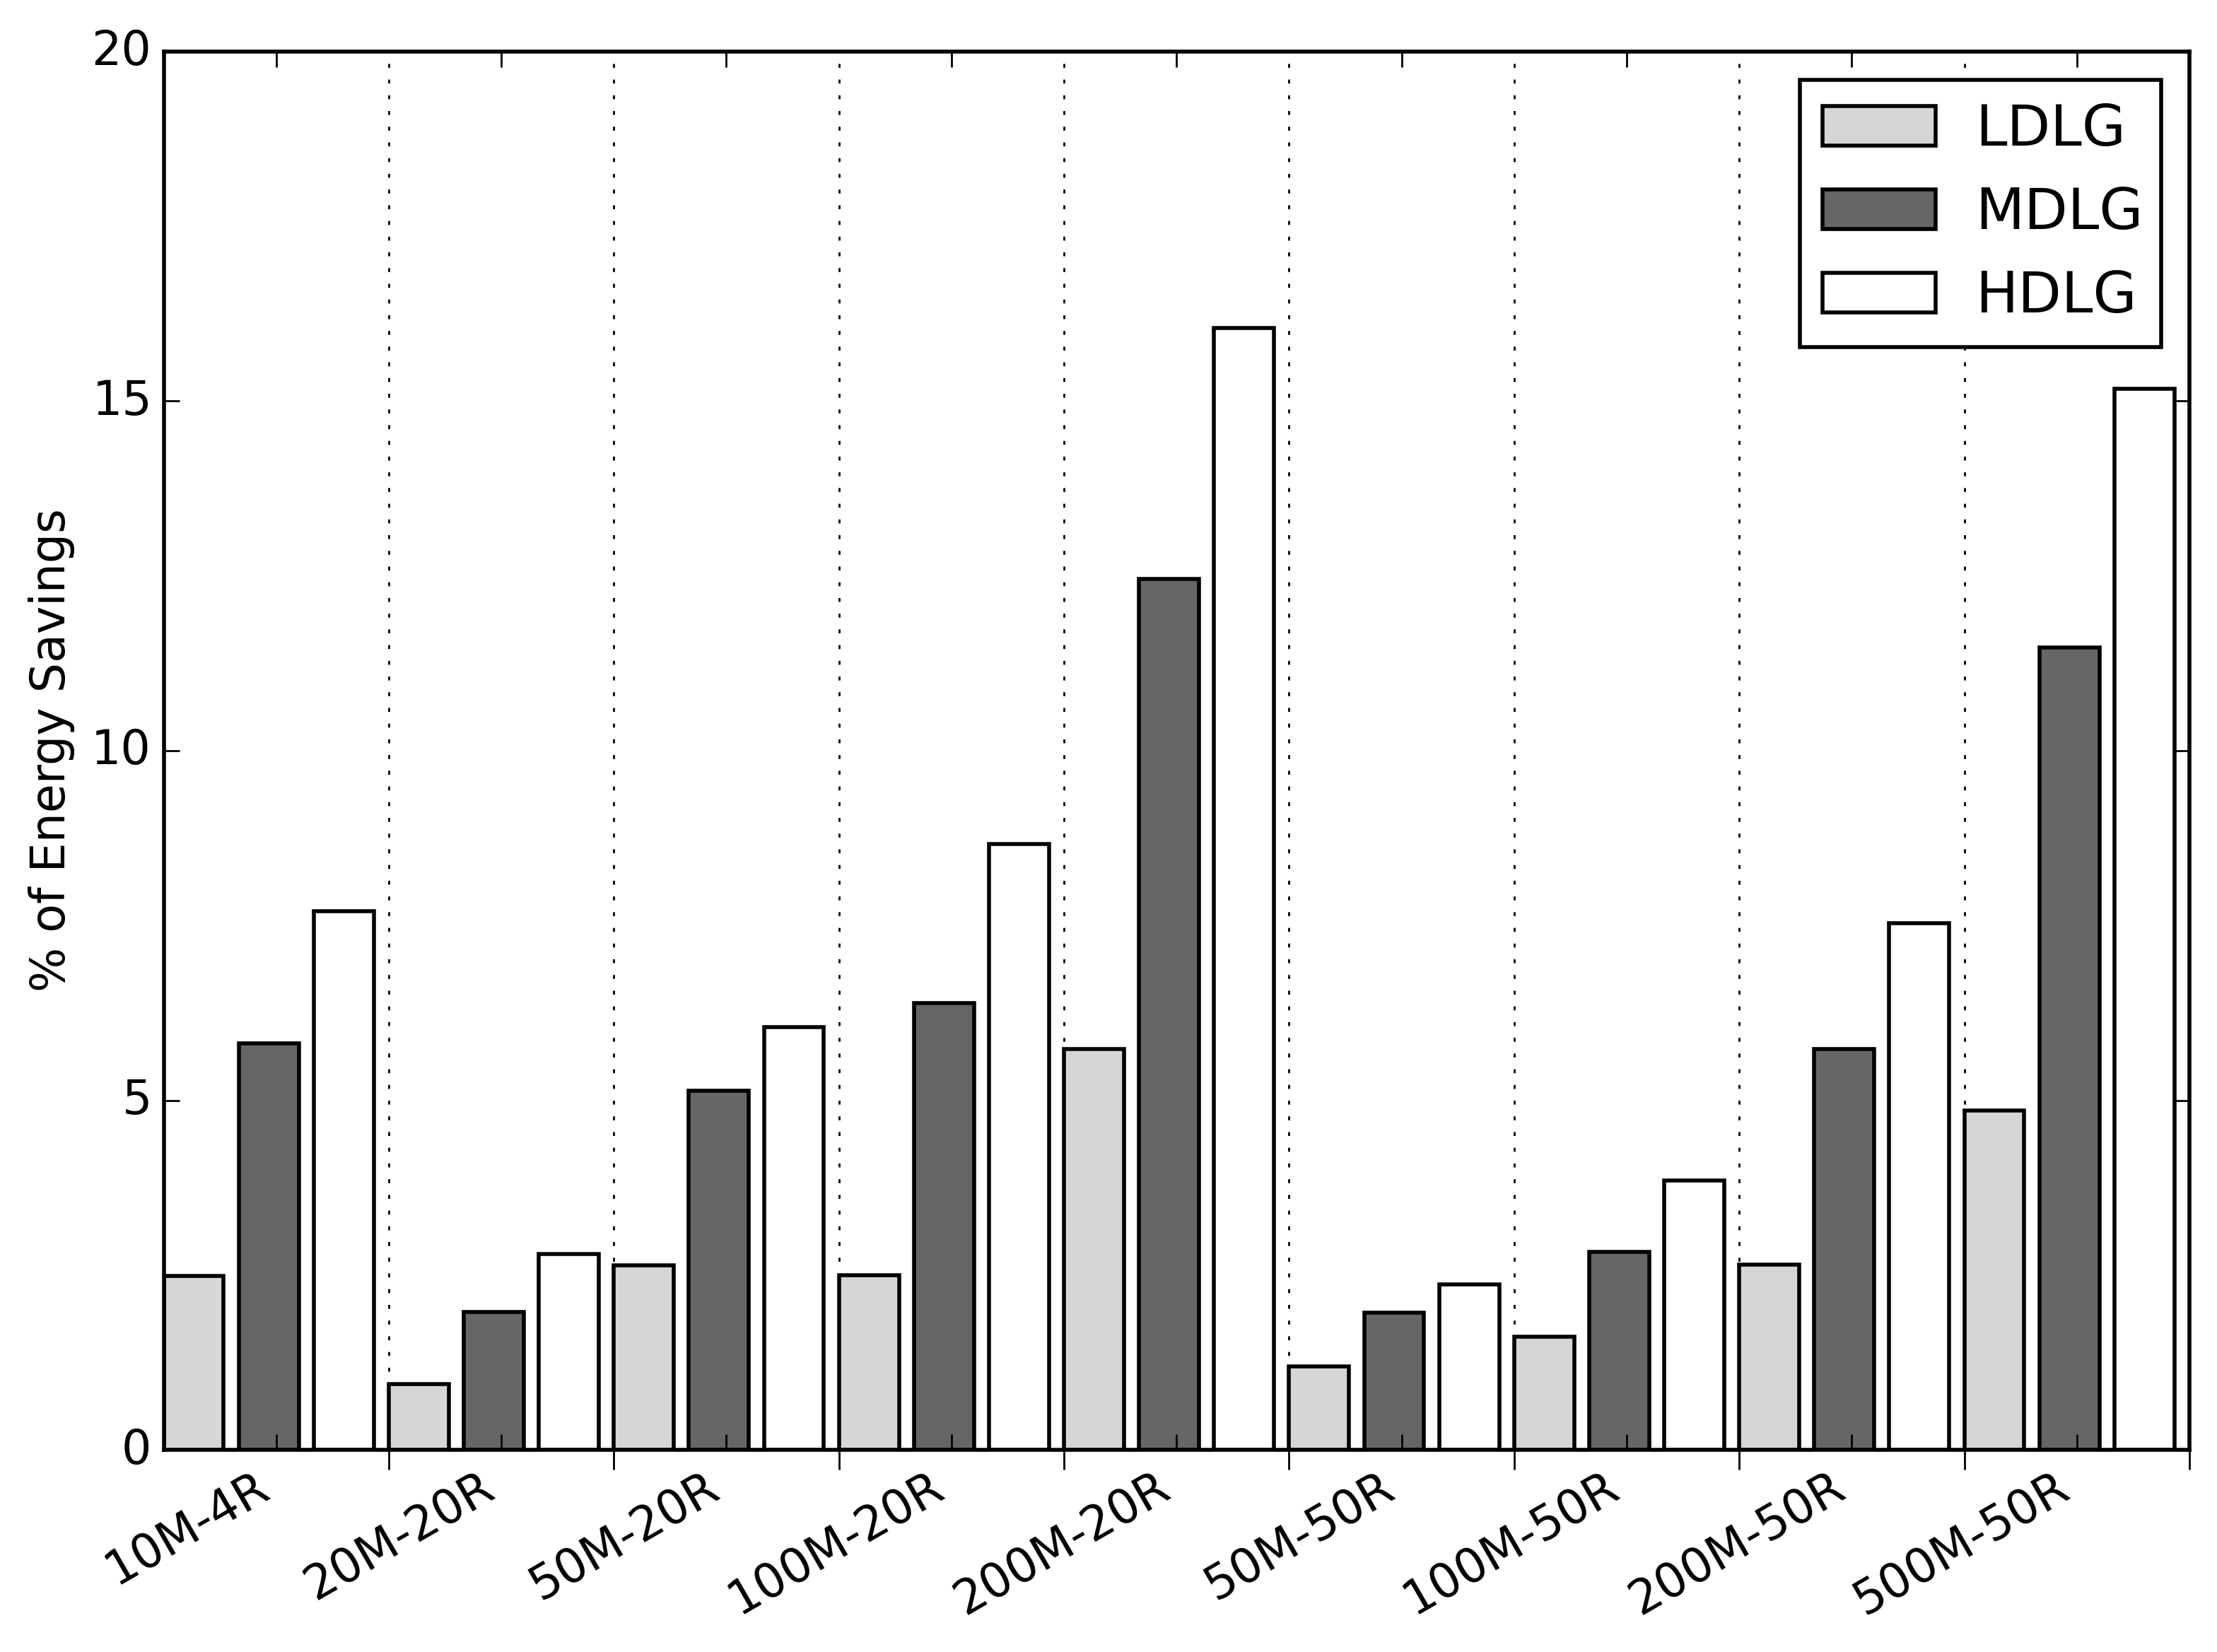
\includegraphics[width=0.9\linewidth]{figs/perc_energy_diff_temp_flex_def_vs_oarb_mtd.png} \\
(a) Maximum temperature deviation aware approach \\[6pt]
  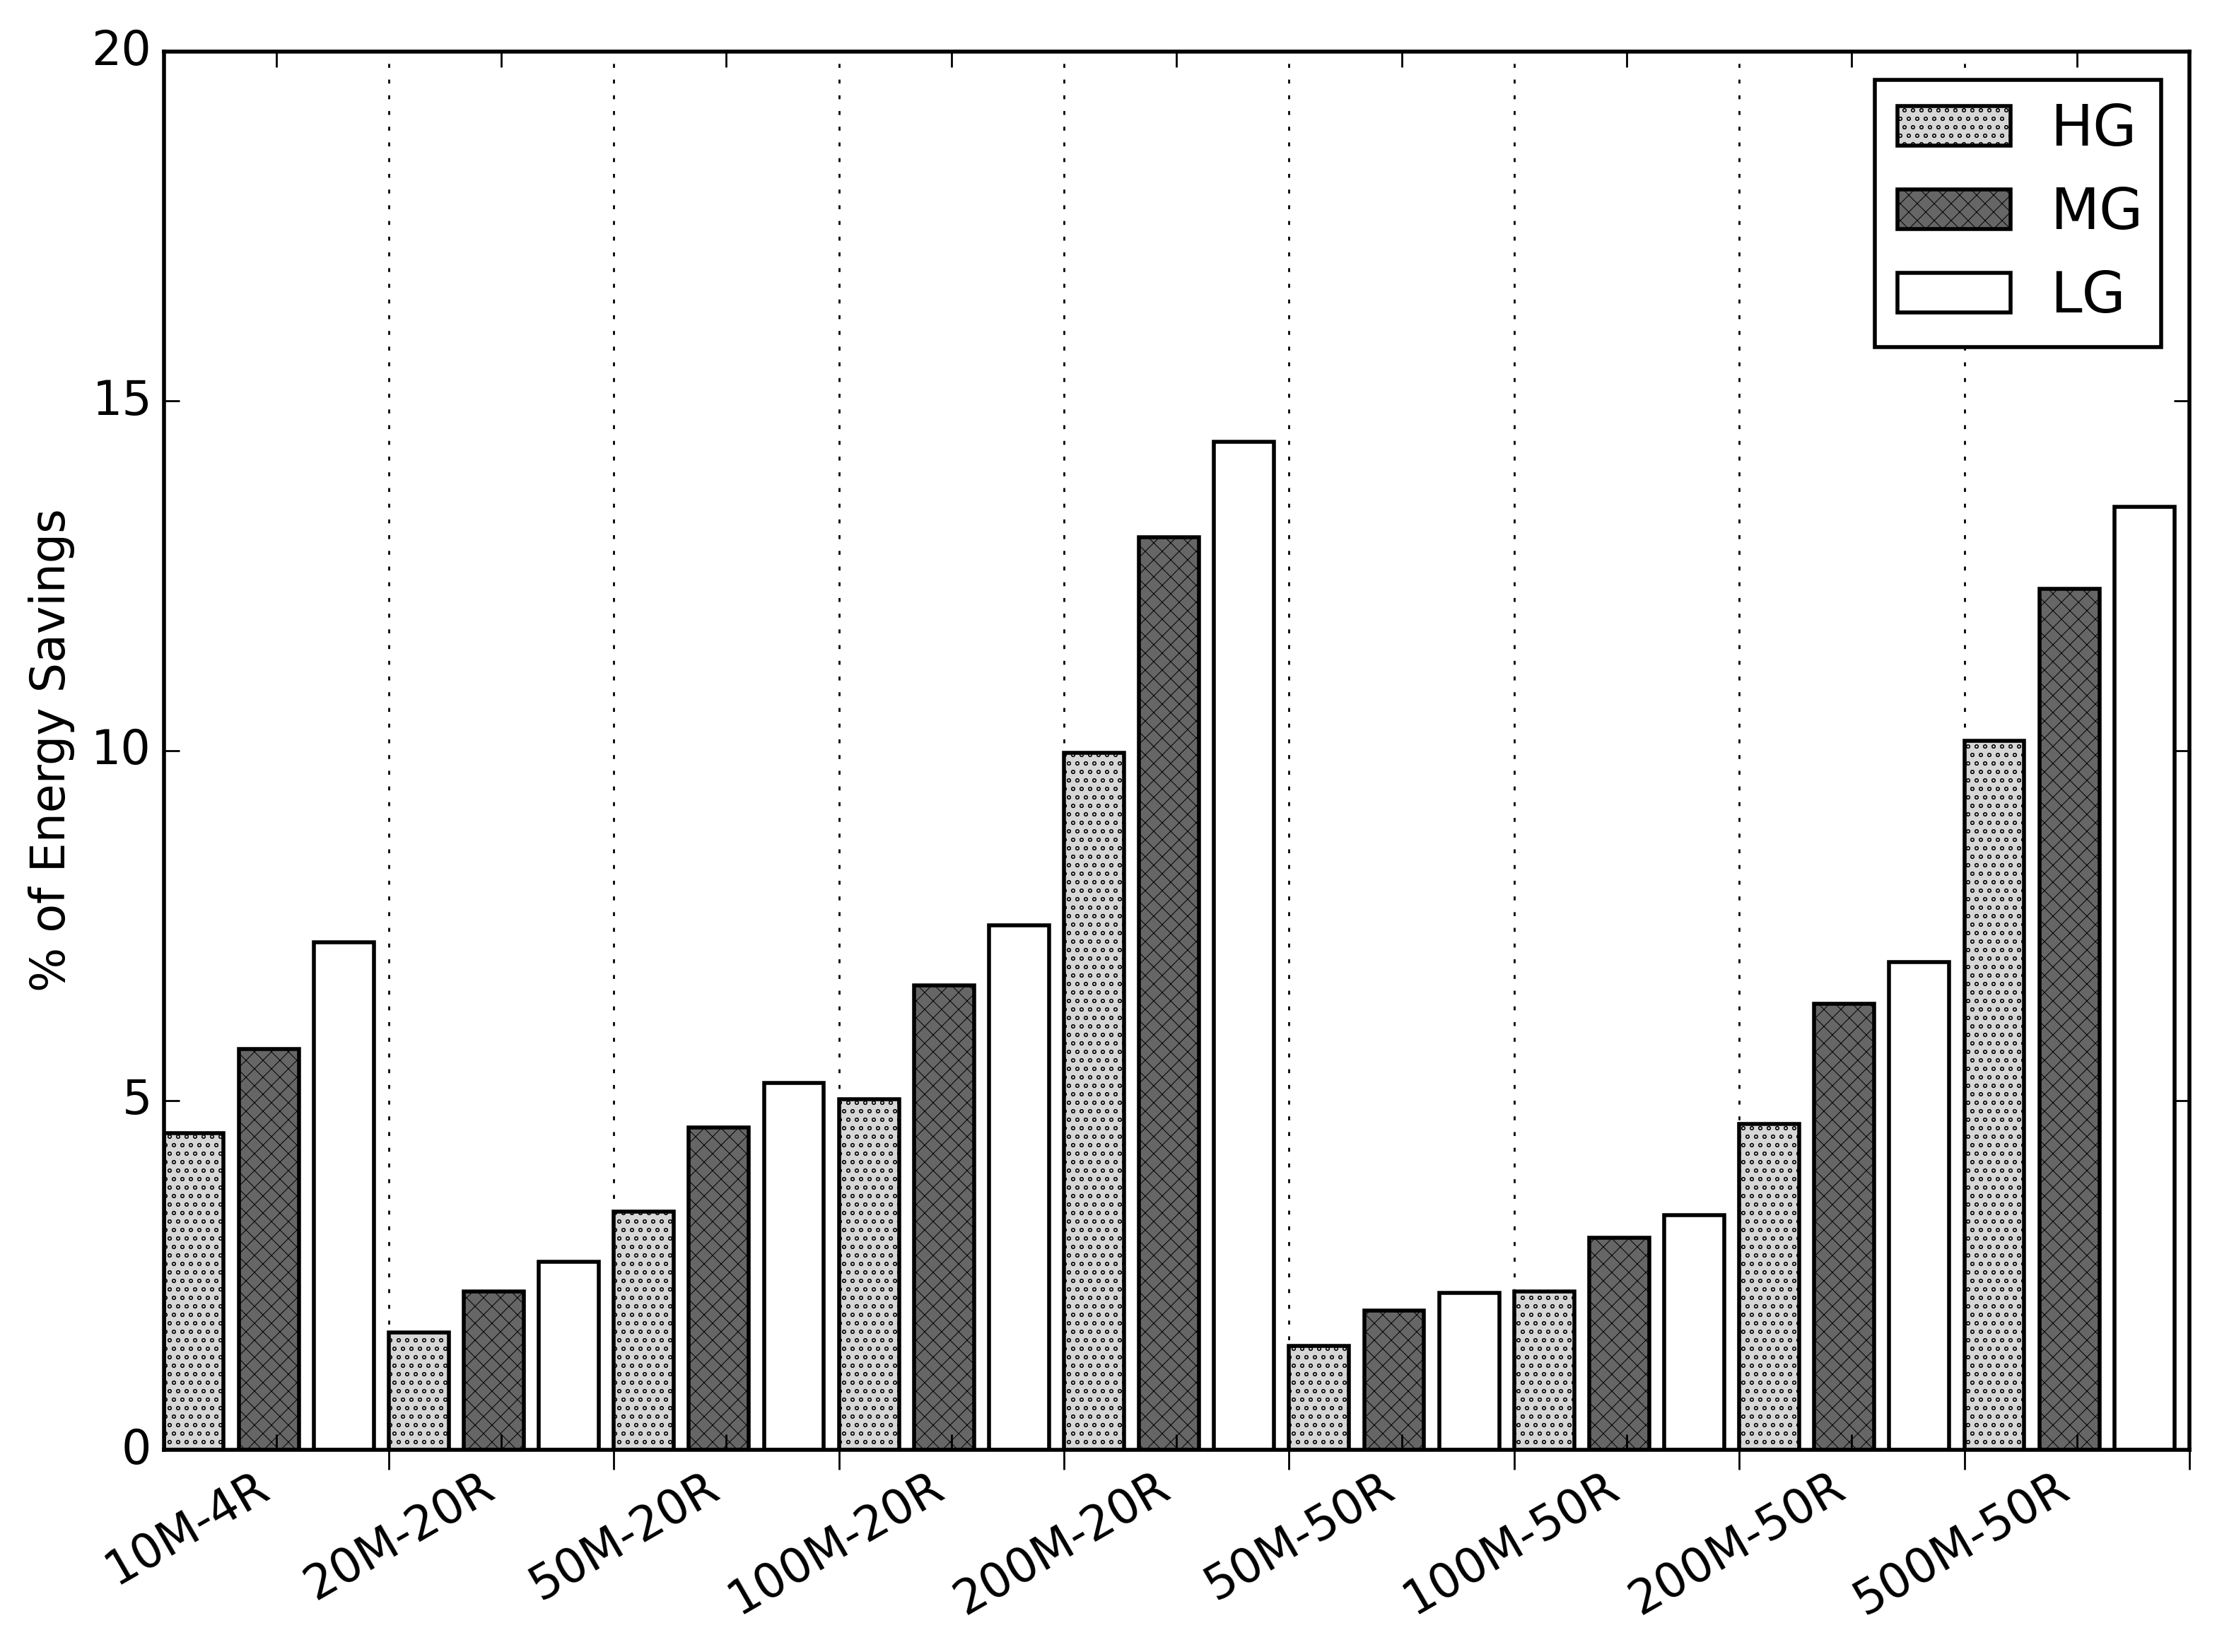
\includegraphics[width=0.9\linewidth]{figs/perc_energy_diff_temp_flex_def_vs_oarb_oat.png} \\
(b) Outdoor temperature aware approach \\[6pt]
\end{tabular}
\caption{Energy savings from adaptive temperature control}
\label{fig:atc_eg}
\end{figure}

\begin{figure}
\centering
%[   44.47609694    51.07362773    59.69232313    56.26772727    46.89050505
    %94.85306626   205.17049756   210.85962697   256.22409756   303.85022764
   %303.44908271   331.32429174   664.61328571   681.7675       711.93804762
   %199.65863733   143.6149328    235.7897653    340.69581977   324.27152273
   %345.71066304   662.44982143   707.63025      731.36820122  1510.82742944
  %1545.13683284  1617.978348  ]
%[  4.33243414   4.97510222   5.81465274   1.17189453   0.97659402
   %1.97551589   4.11101854   4.22501211   5.13398383   5.85823739
   %5.85050331   6.3879378   11.62851785  11.92865944  12.45654348
   %1.66661057   1.19879695   1.96820794   2.78713168   2.65276936
   %2.82815663   5.1909067    5.54493712   5.73094591  10.71686841
  %10.96023794  11.47693026]
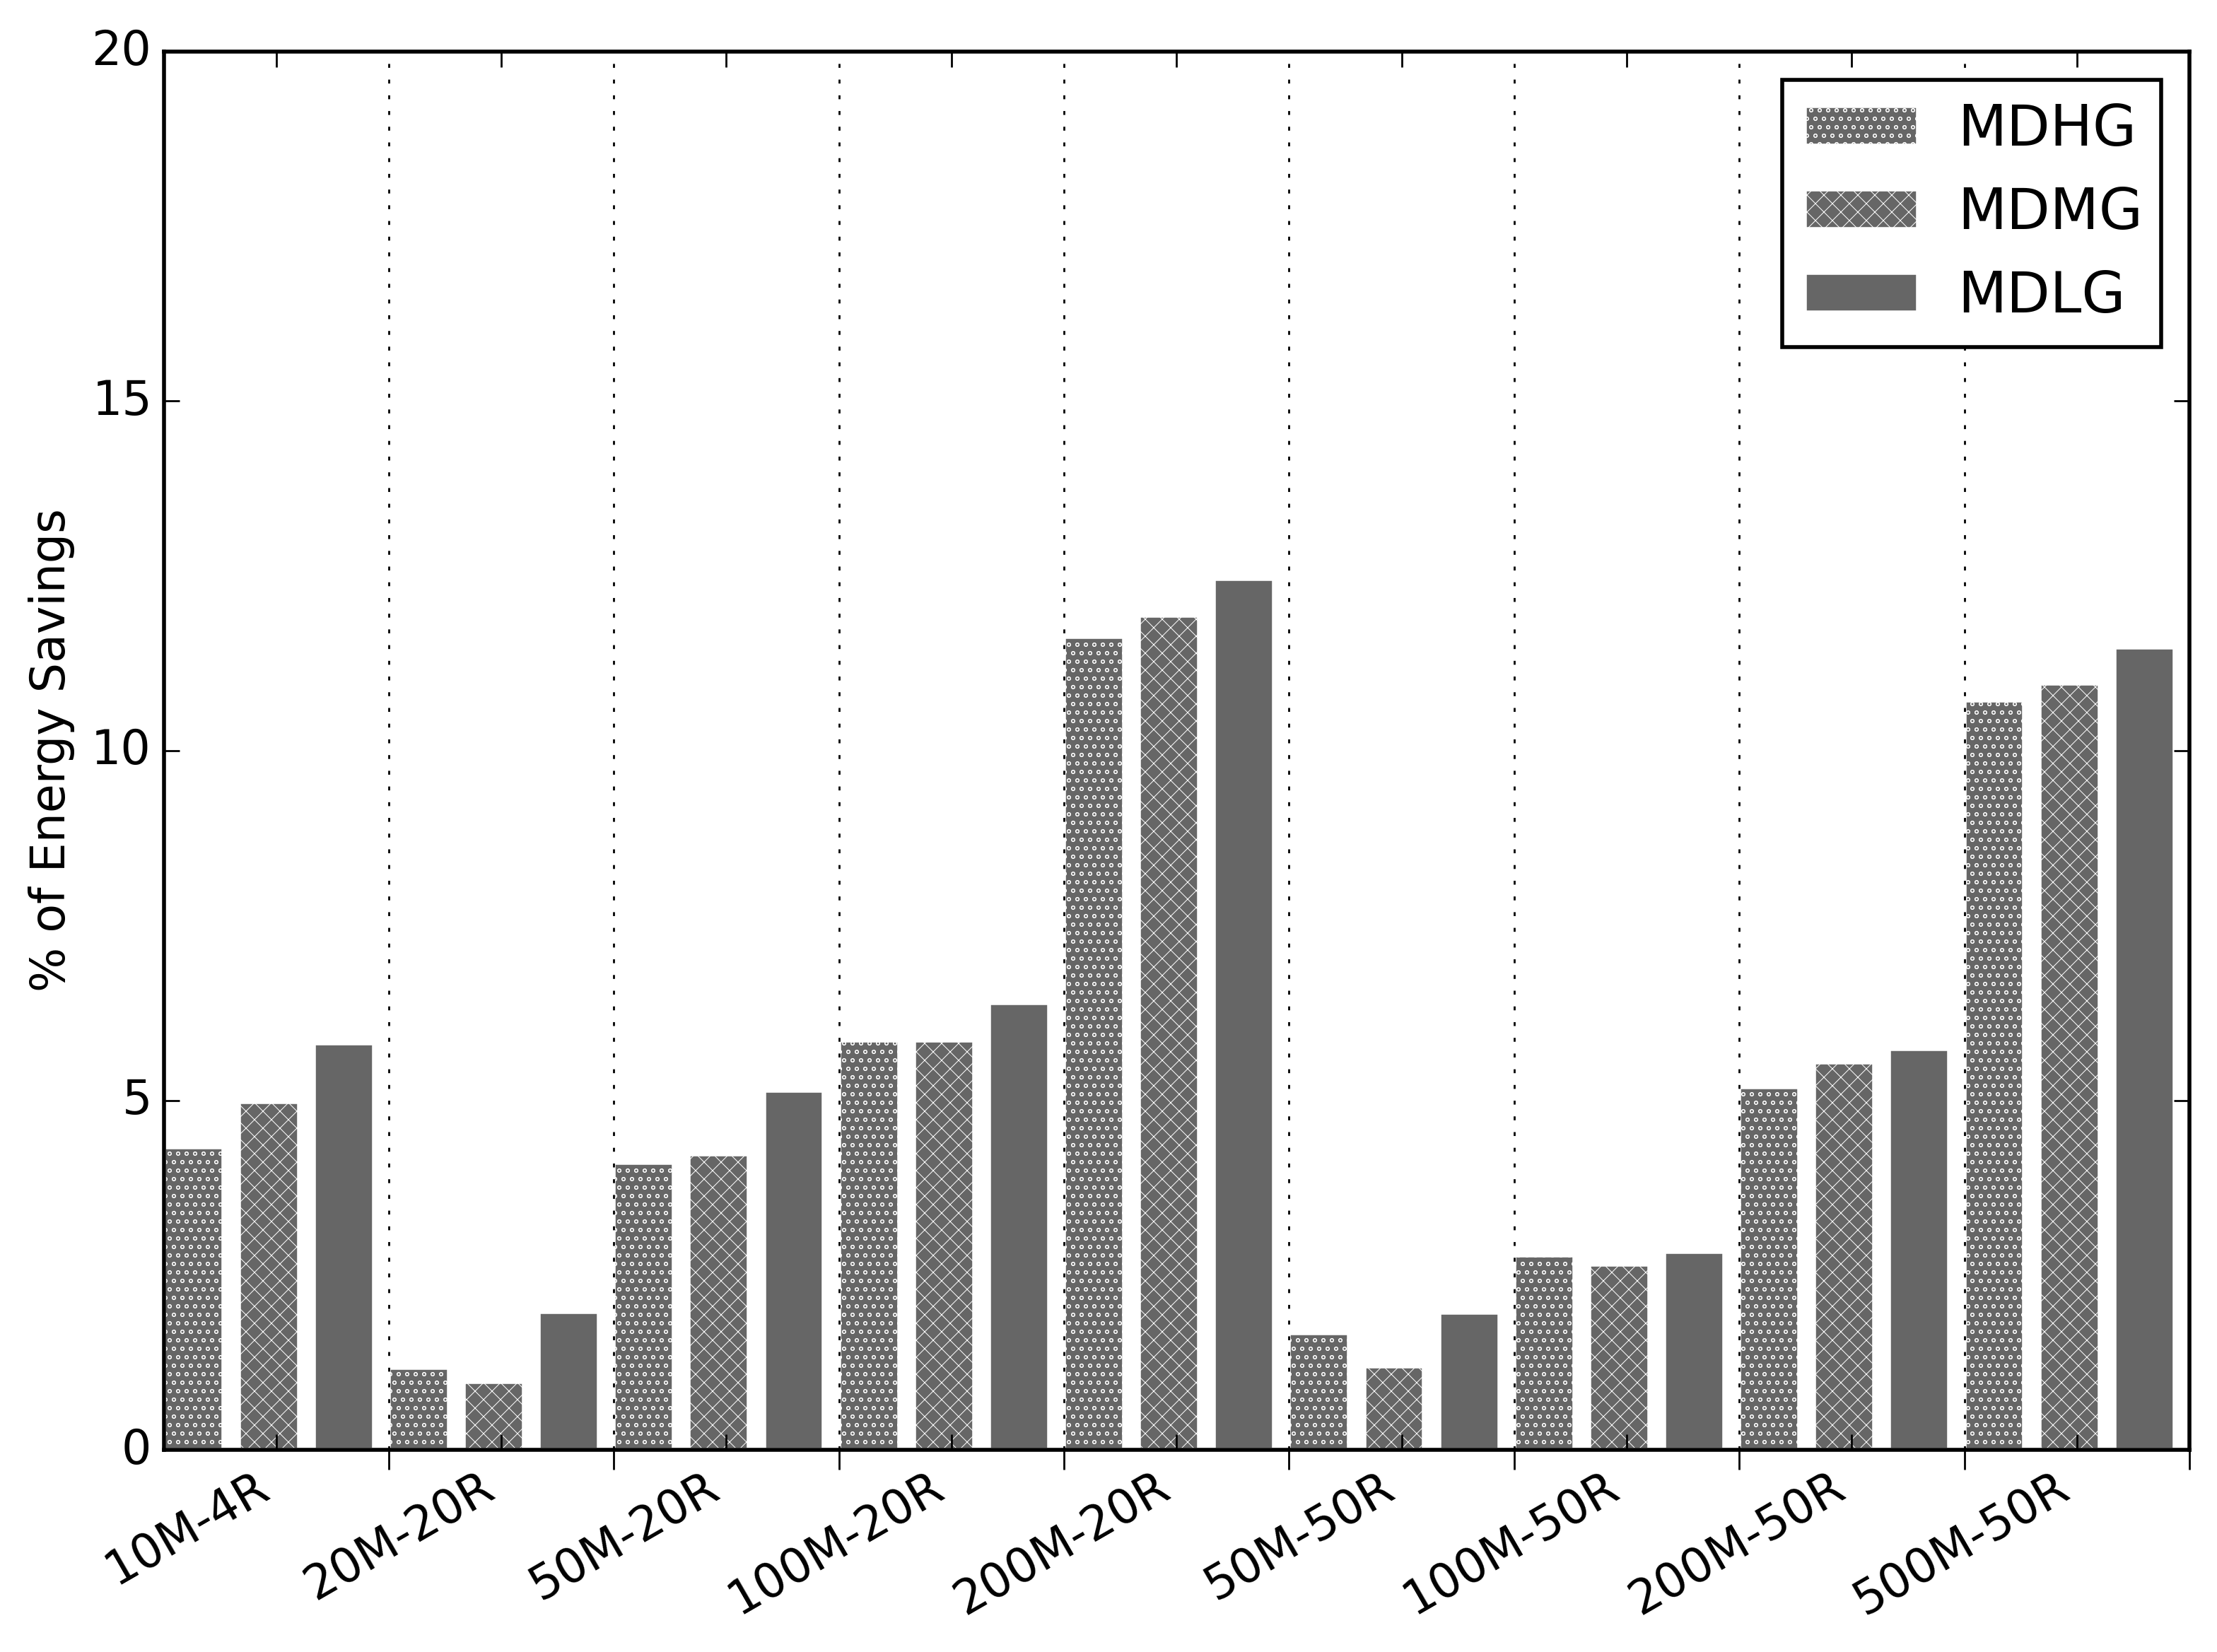
\includegraphics[width=0.9\linewidth]{figs/perc_energy_diff_temp_flex_def_vs_oarb_medium_mtd.png}	
\caption{MTDA approach - energy savings (Medium Deviation)}
\label{fig:atc_memr}
\end{figure}

\begin{figure}
\centering
%[   69.64202826    71.84756672    79.06680864   105.85977645   121.69272727
   %134.53116477   280.12787175   280.90855658   302.02851692   396.06496838
   %405.90309669   449.57078678   852.79995745   832.23765385   916.90629508
   %218.07404962   205.60479675   284.13228309   332.21576961   342.75882547
   %471.03871721   847.64491667   776.96237245   961.99058333  2085.35333017
  %2127.82956012  2138.9962836 ]
%[  6.78385744   6.99869981   7.70192901   2.20475392   2.53450864
   %2.80189628   5.61294577   5.62858841   6.05177084   7.63613911
   %7.82581839   8.66773217  14.92115752  14.56138573  16.04280481
   %1.82032954   1.71624495   2.37173744   2.7177589    2.80400852
   %3.85342835   6.64208145   6.08821838   7.53808545  14.79219717
  %15.09349708  15.17270686]
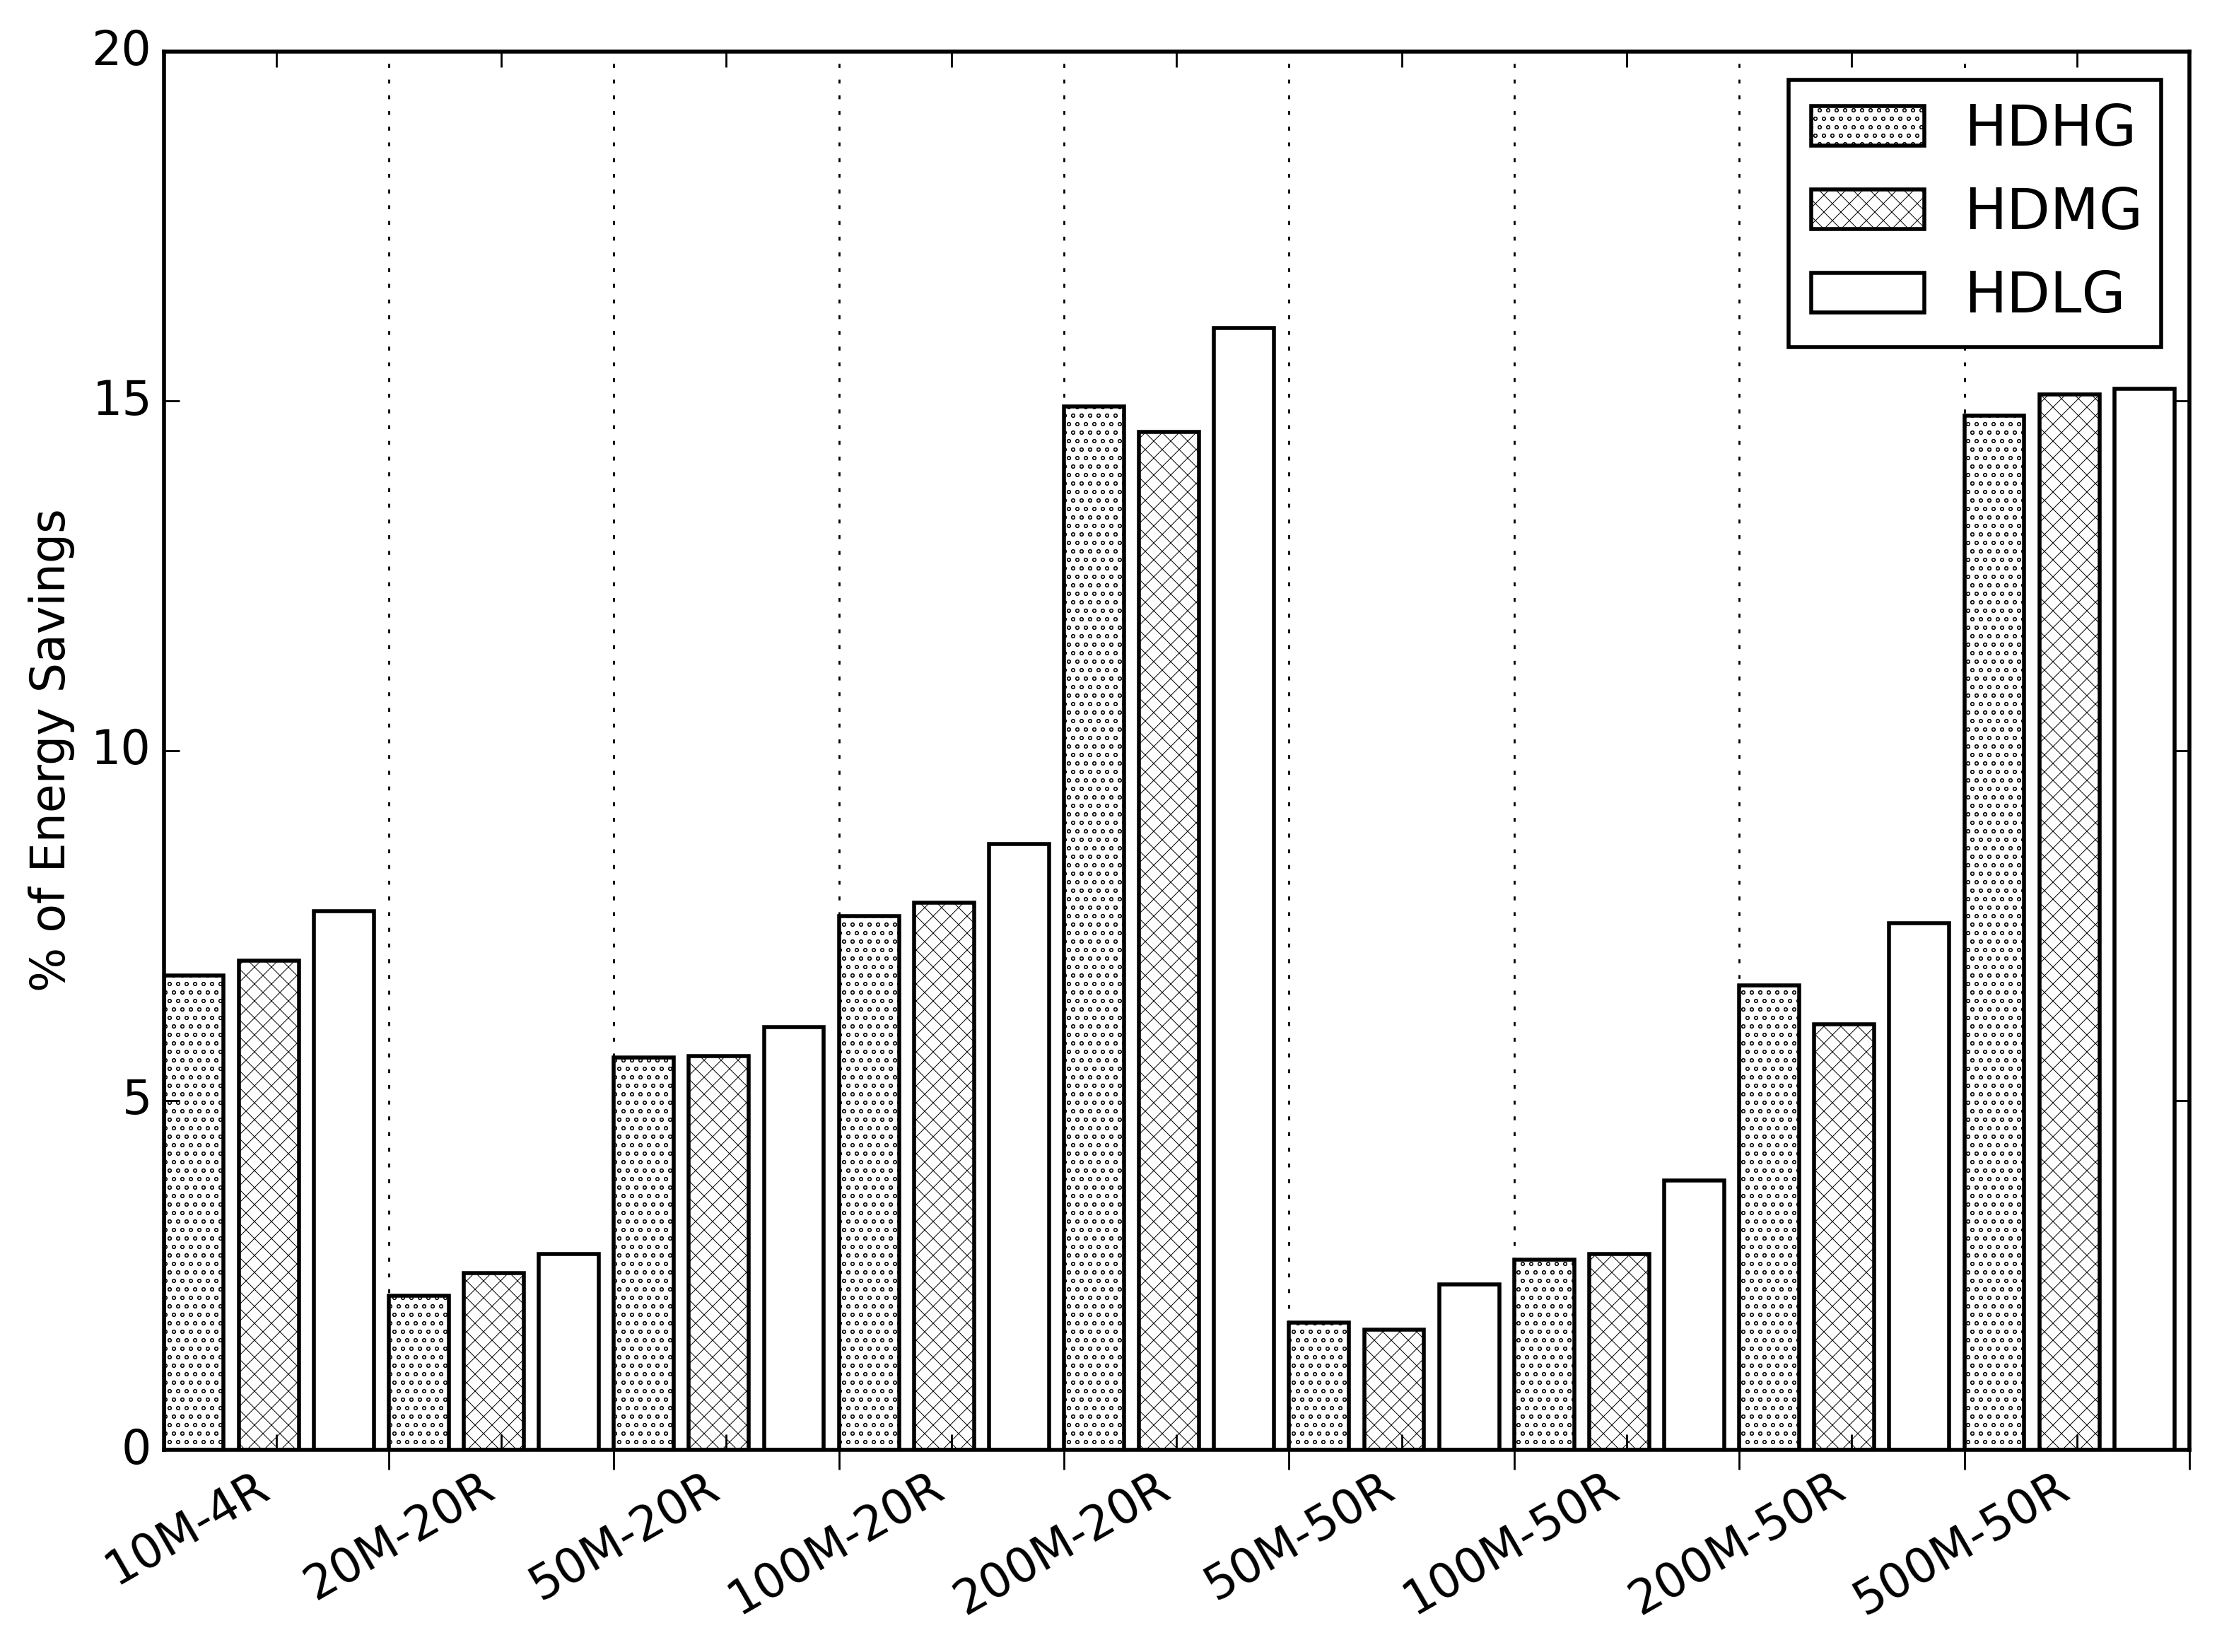
\includegraphics[width=0.9\linewidth]{figs/perc_energy_diff_temp_flex_def_vs_oarb_high_mtd.png}	
\caption{MTDA approach - energy savings (High Deviation)}
\label{fig:atc_mehr}
\end{figure}


\subsection{Effects to Thermal Comfort} \label{sec:atc_comfort}

\begin{figure}
\centering
\begin{tabular}{c}
  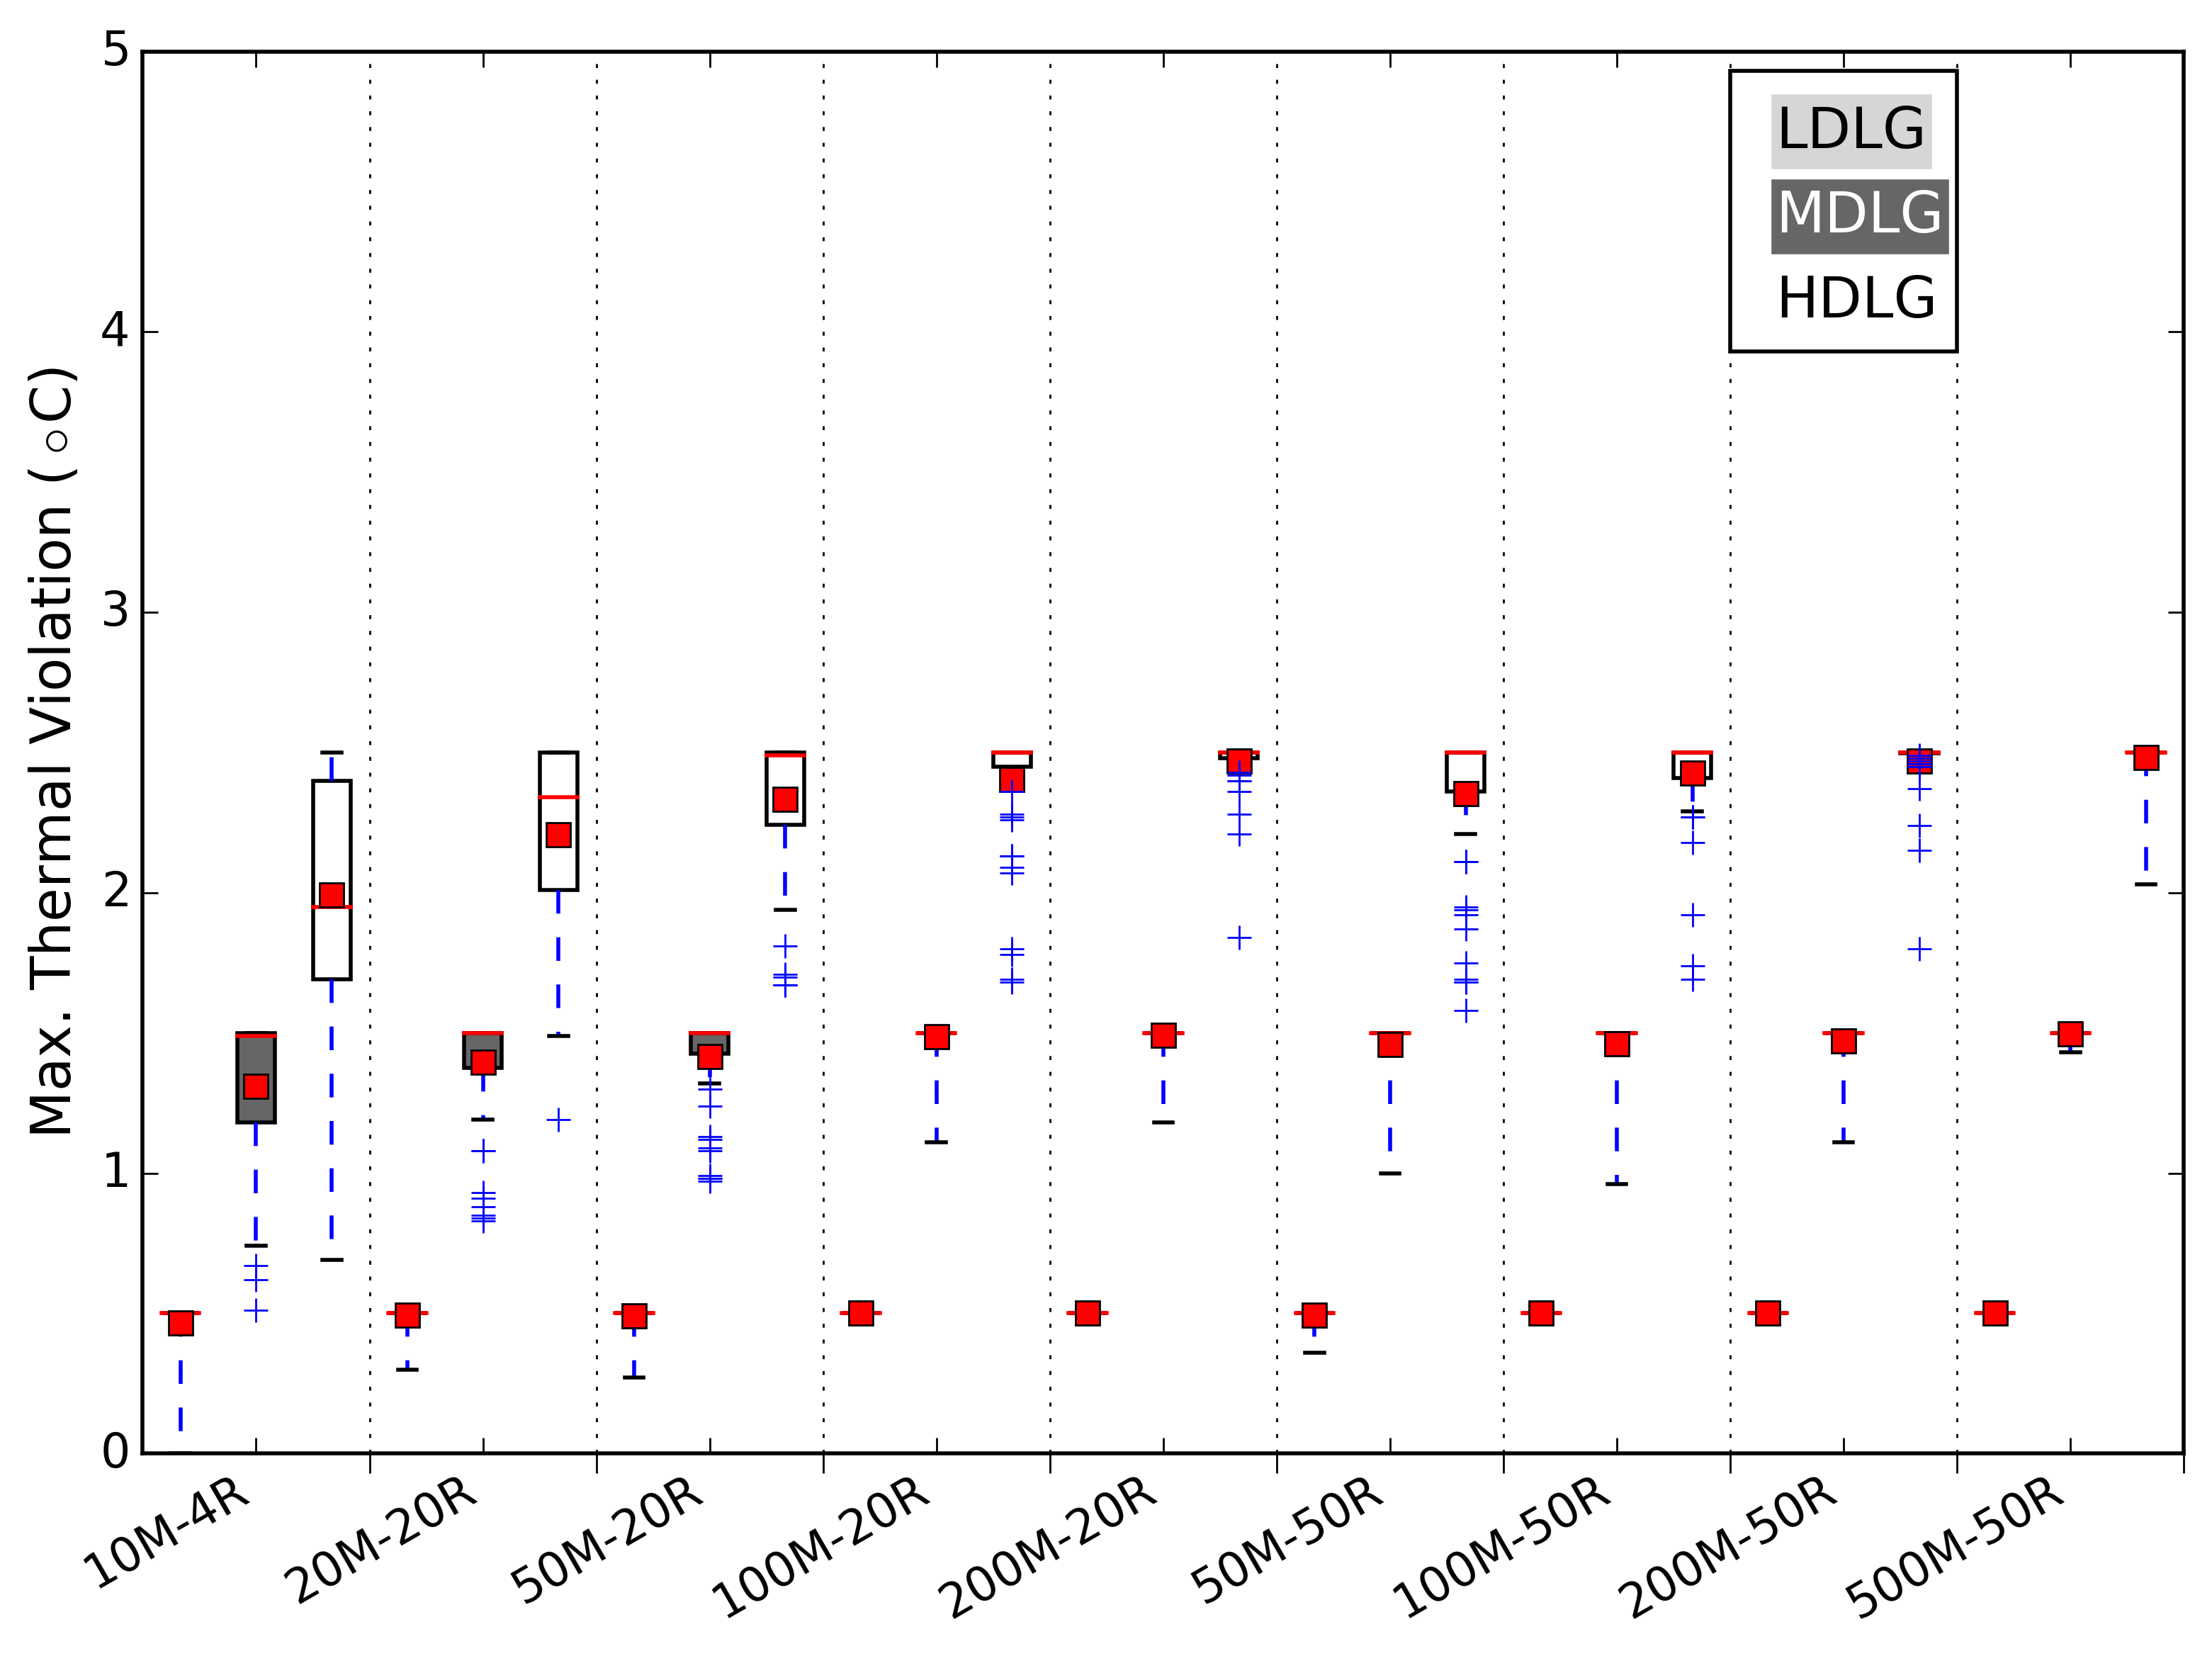
\includegraphics[width=0.6\linewidth]{figs/max_thermal_violation_diff_temp_flex_def_vs_oarb_boxplot_mtd.png} \\
(a) Maximum \\[6pt]
  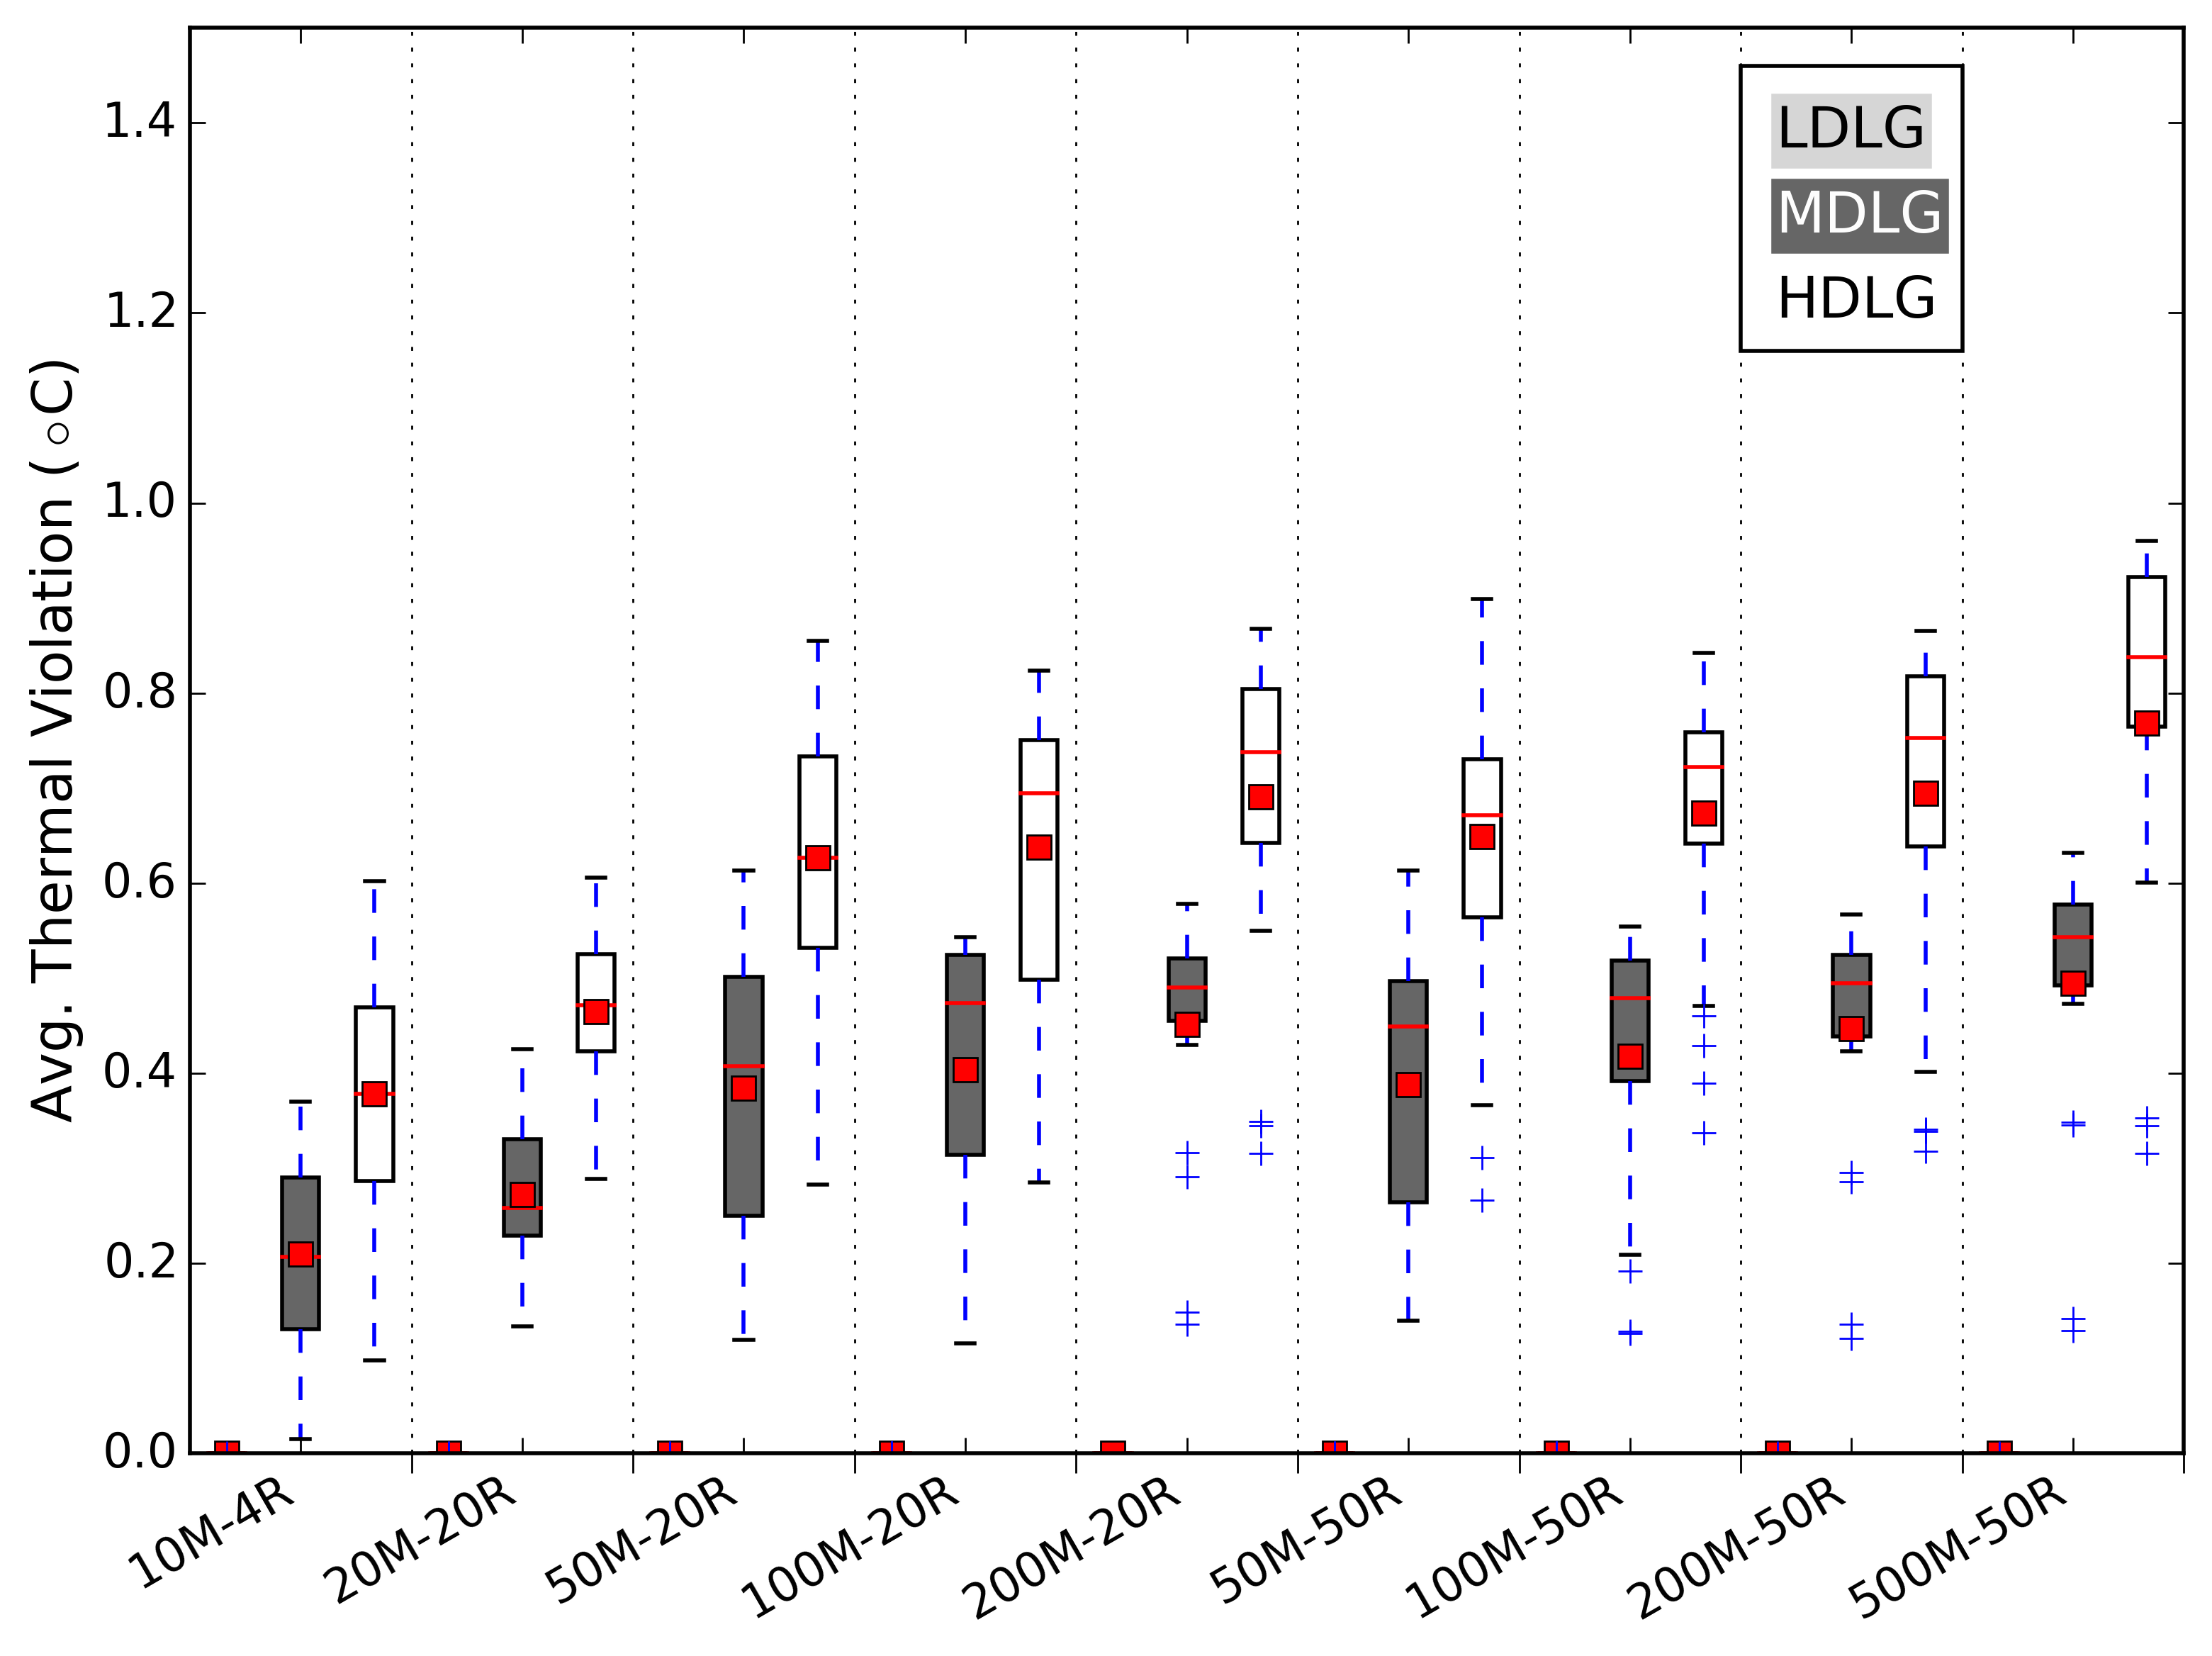
\includegraphics[width=0.6\linewidth]{figs/avg_thermal_violation_diff_temp_flex_def_vs_oarb_boxplot_mtd.png} \\
(b) Average \\[6pt]
	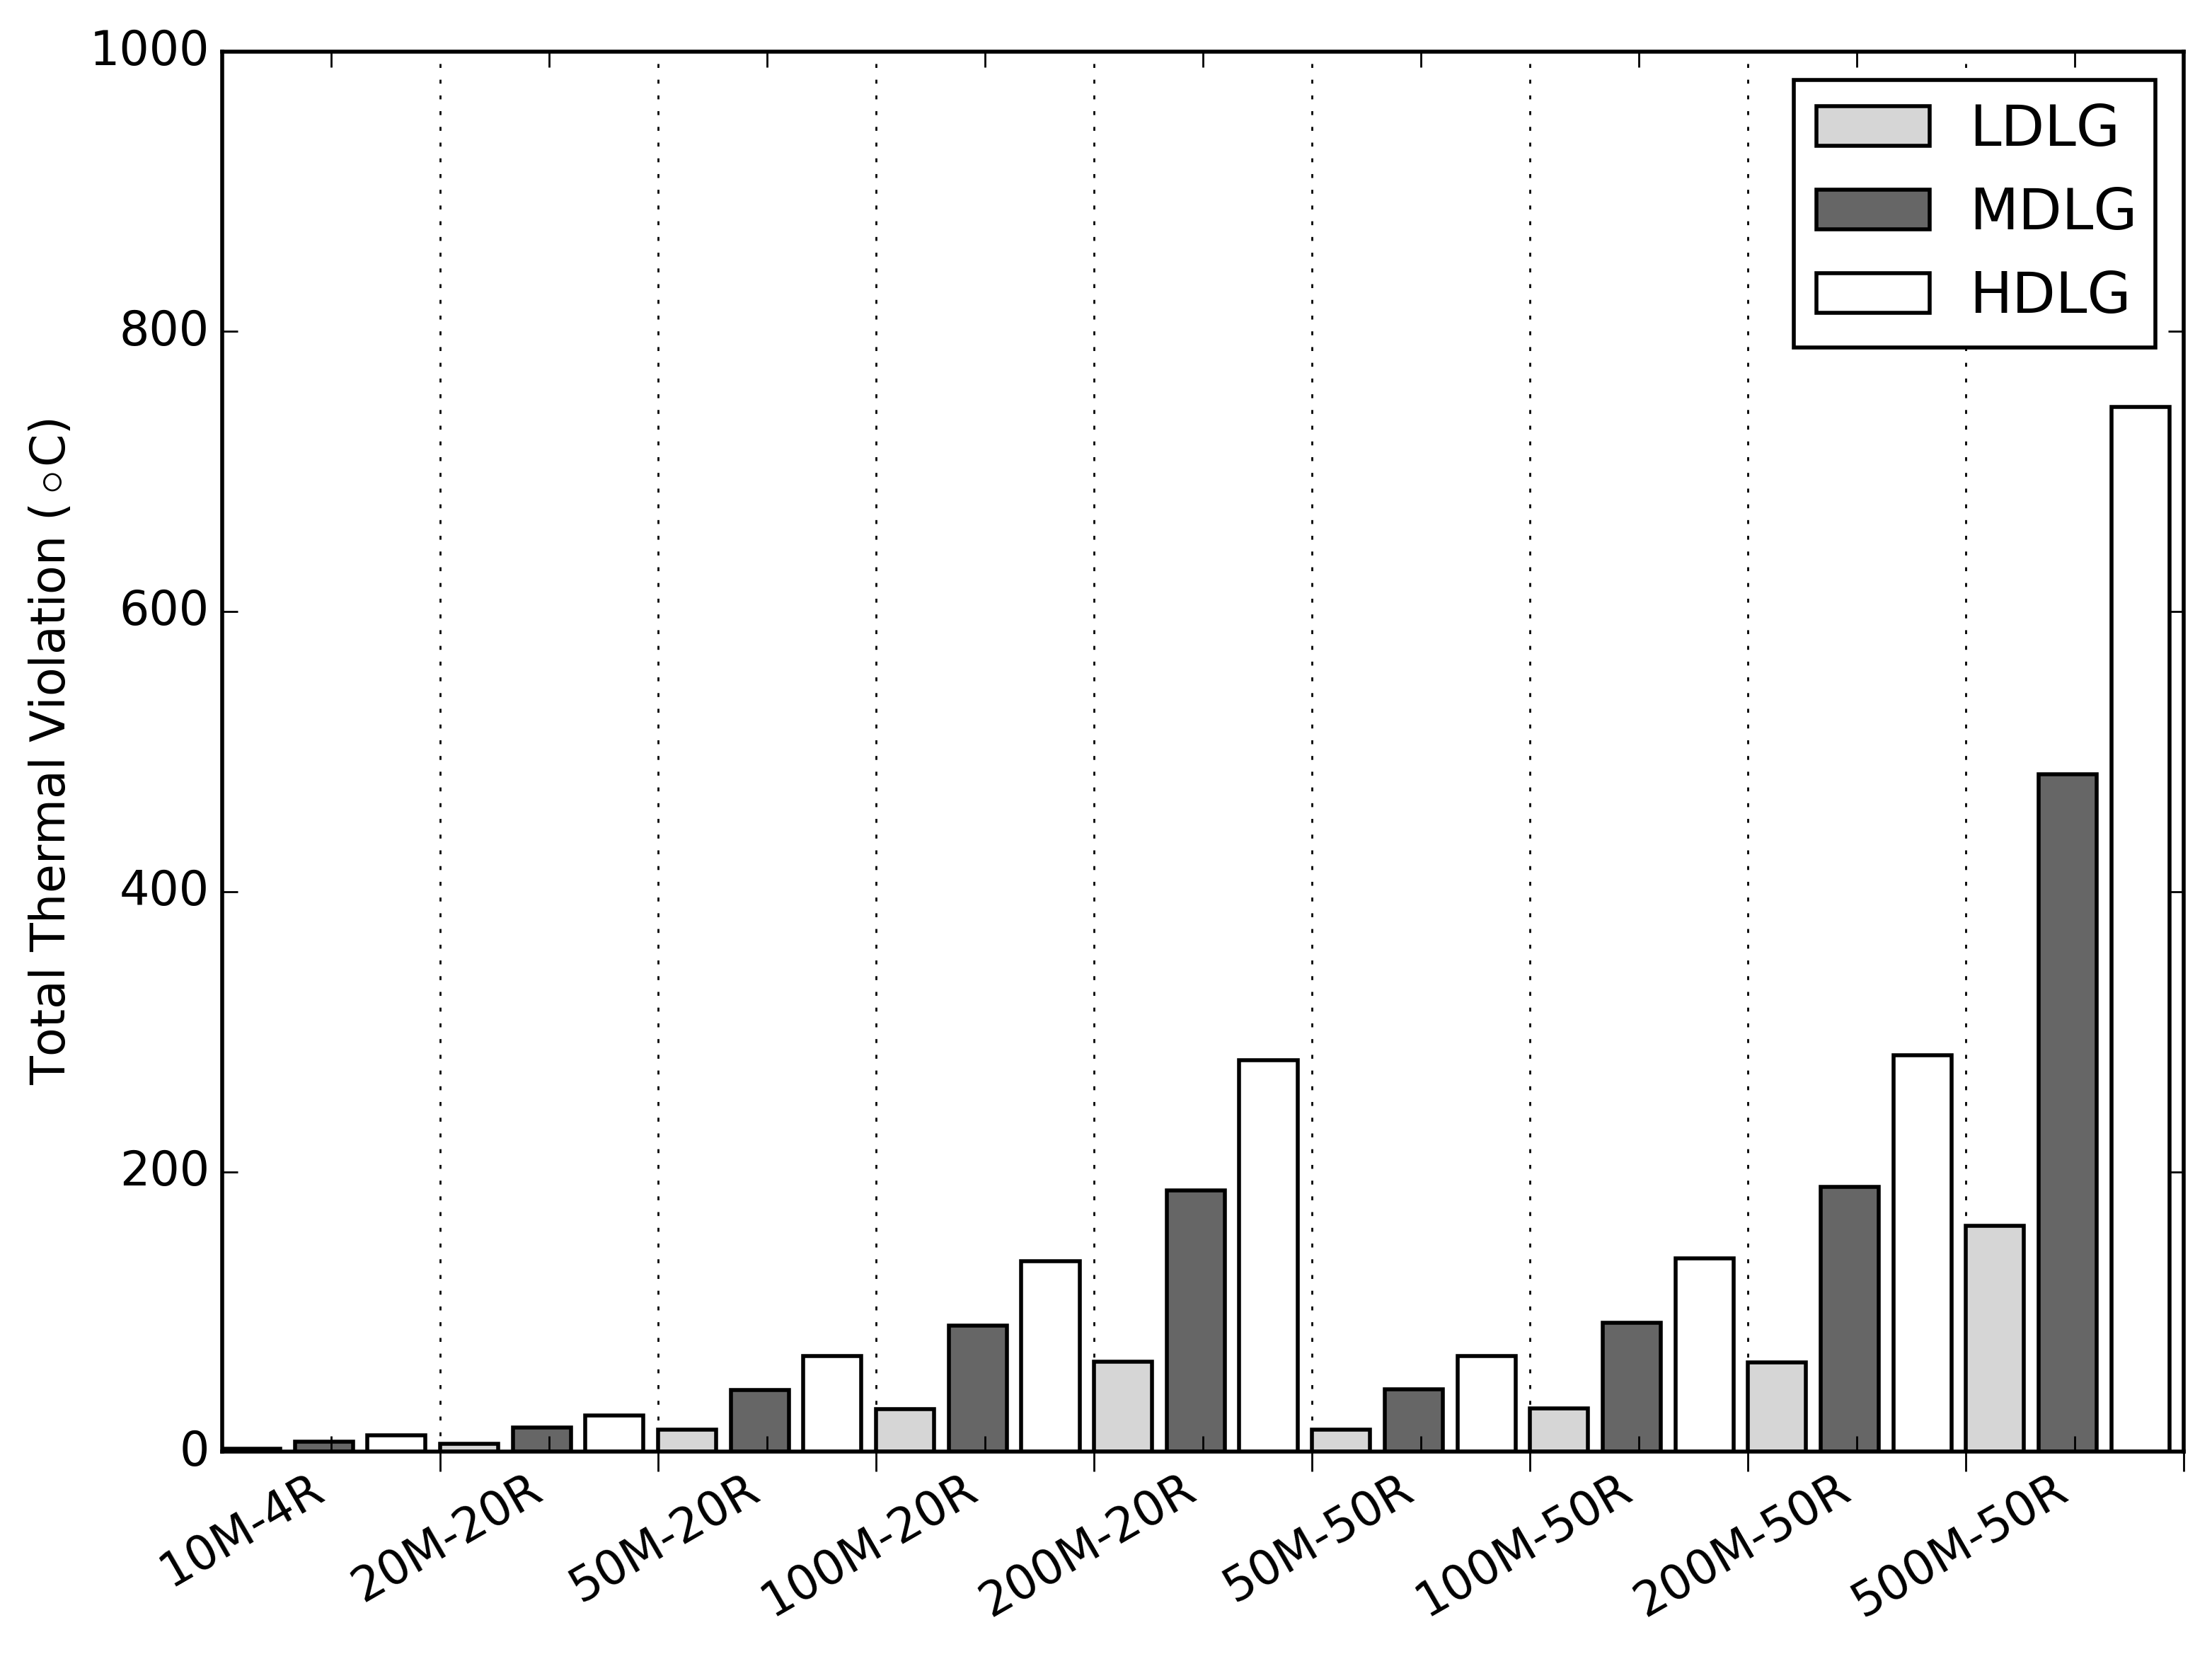
\includegraphics[width=0.6\linewidth]{figs/total_thermal_violation_diff_temp_flex_def_vs_oarb_mtd.png} \\
(c) Total 
\end{tabular}
\caption{Effects to thermal comfort with adaptive temperature control - MTDA approach}
\label{fig:atc_mt}
\end{figure}

\begin{figure}
\centering
\begin{tabular}{c}
  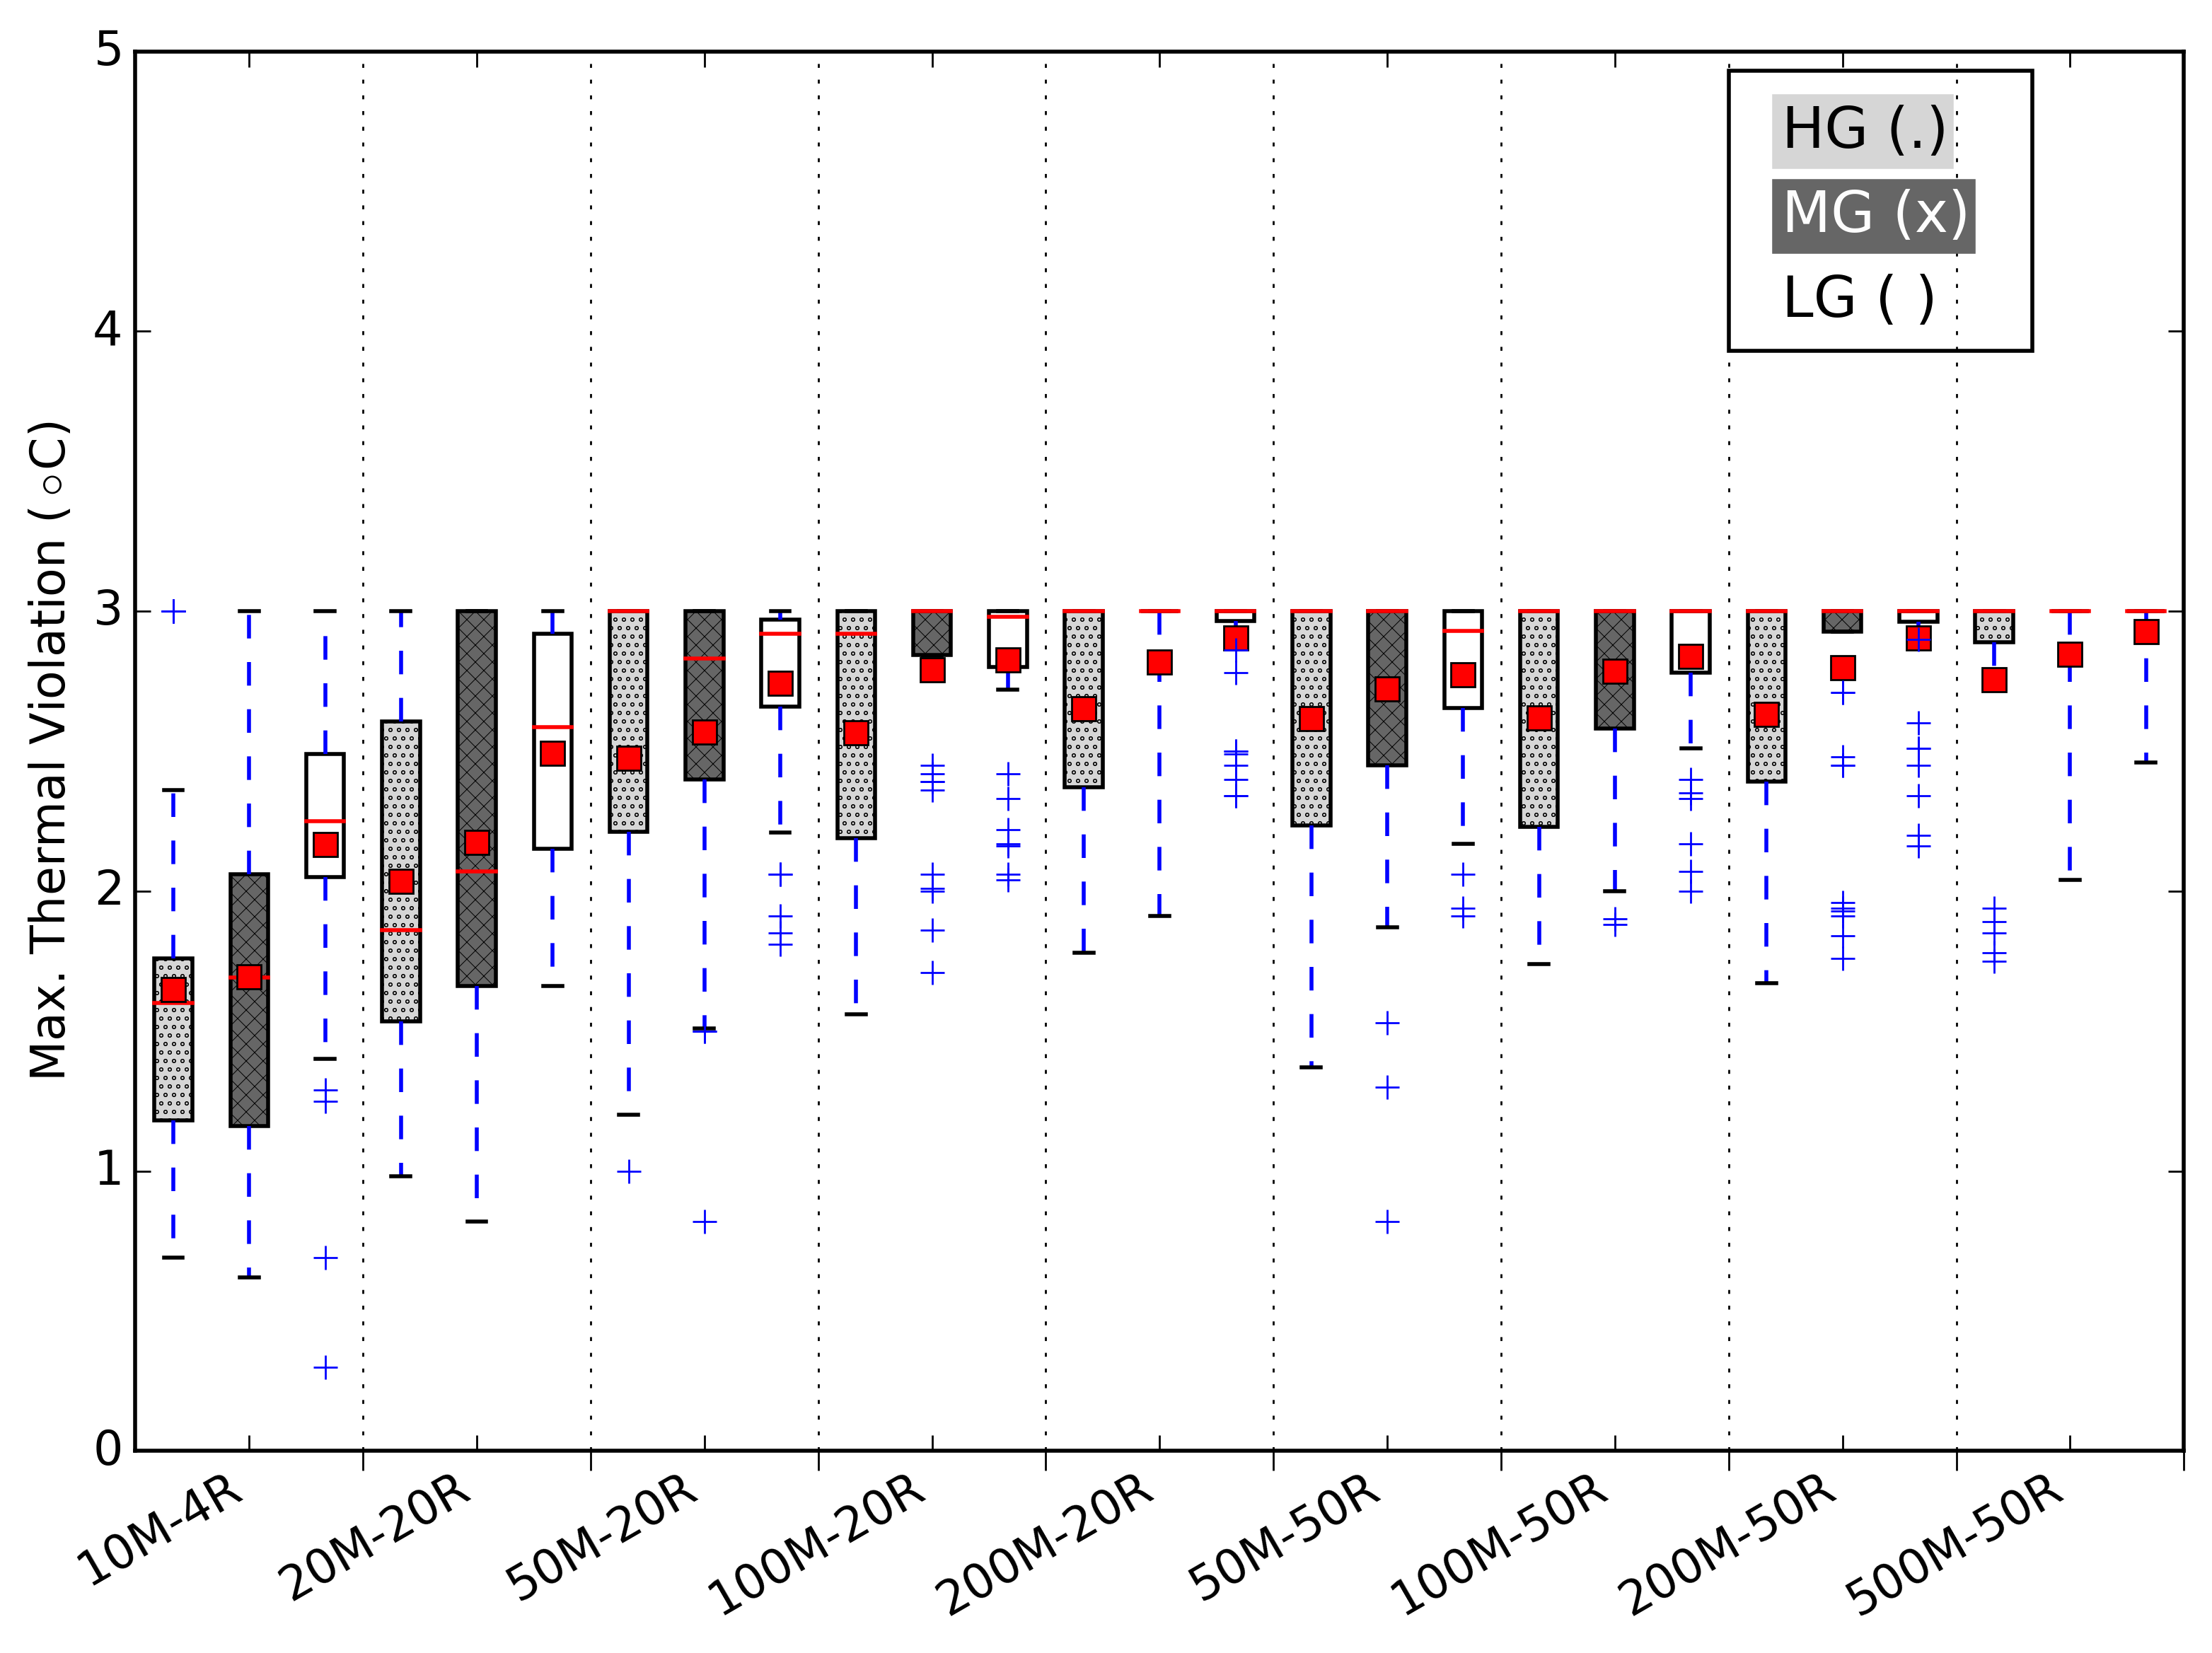
\includegraphics[width=0.6\linewidth]{figs/max_thermal_violation_diff_temp_flex_def_vs_oarb_boxplot_oat.png} \\
(a) Maximum \\[6pt]
  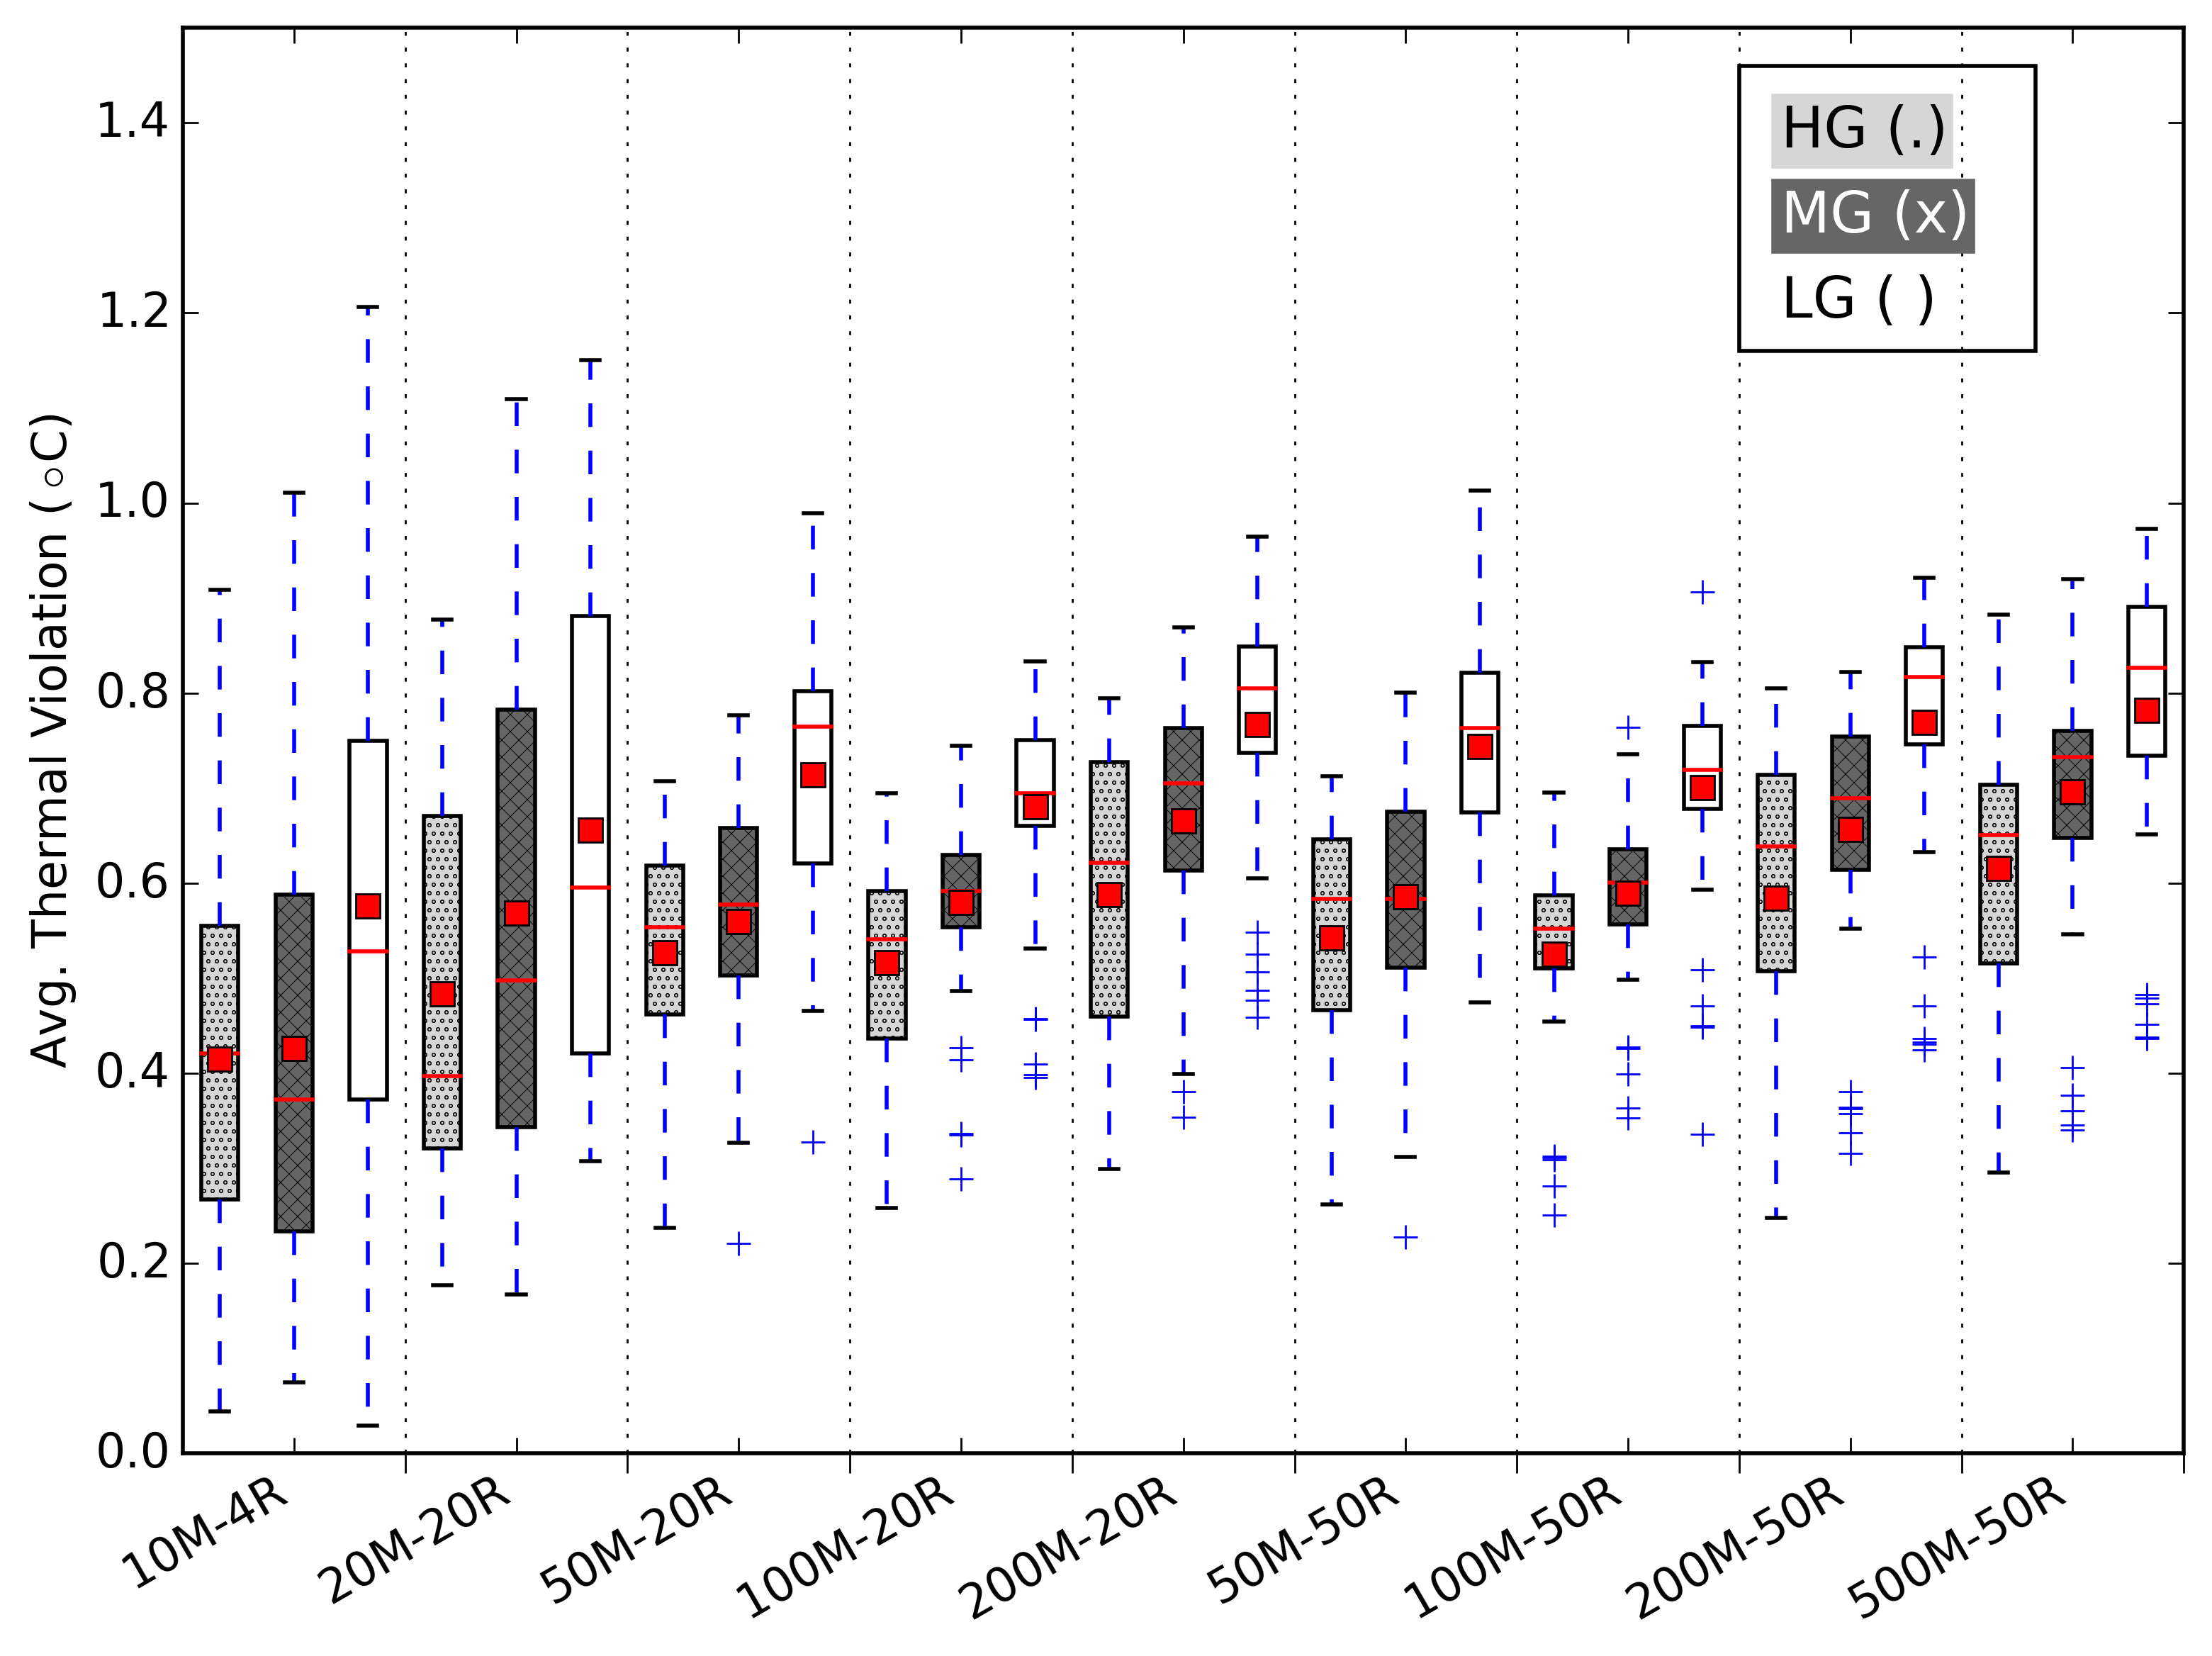
\includegraphics[width=0.6\linewidth]{figs/avg_thermal_violation_diff_temp_flex_def_vs_oarb_boxplot_oat.png} \\
(b) Average \\[6pt]
	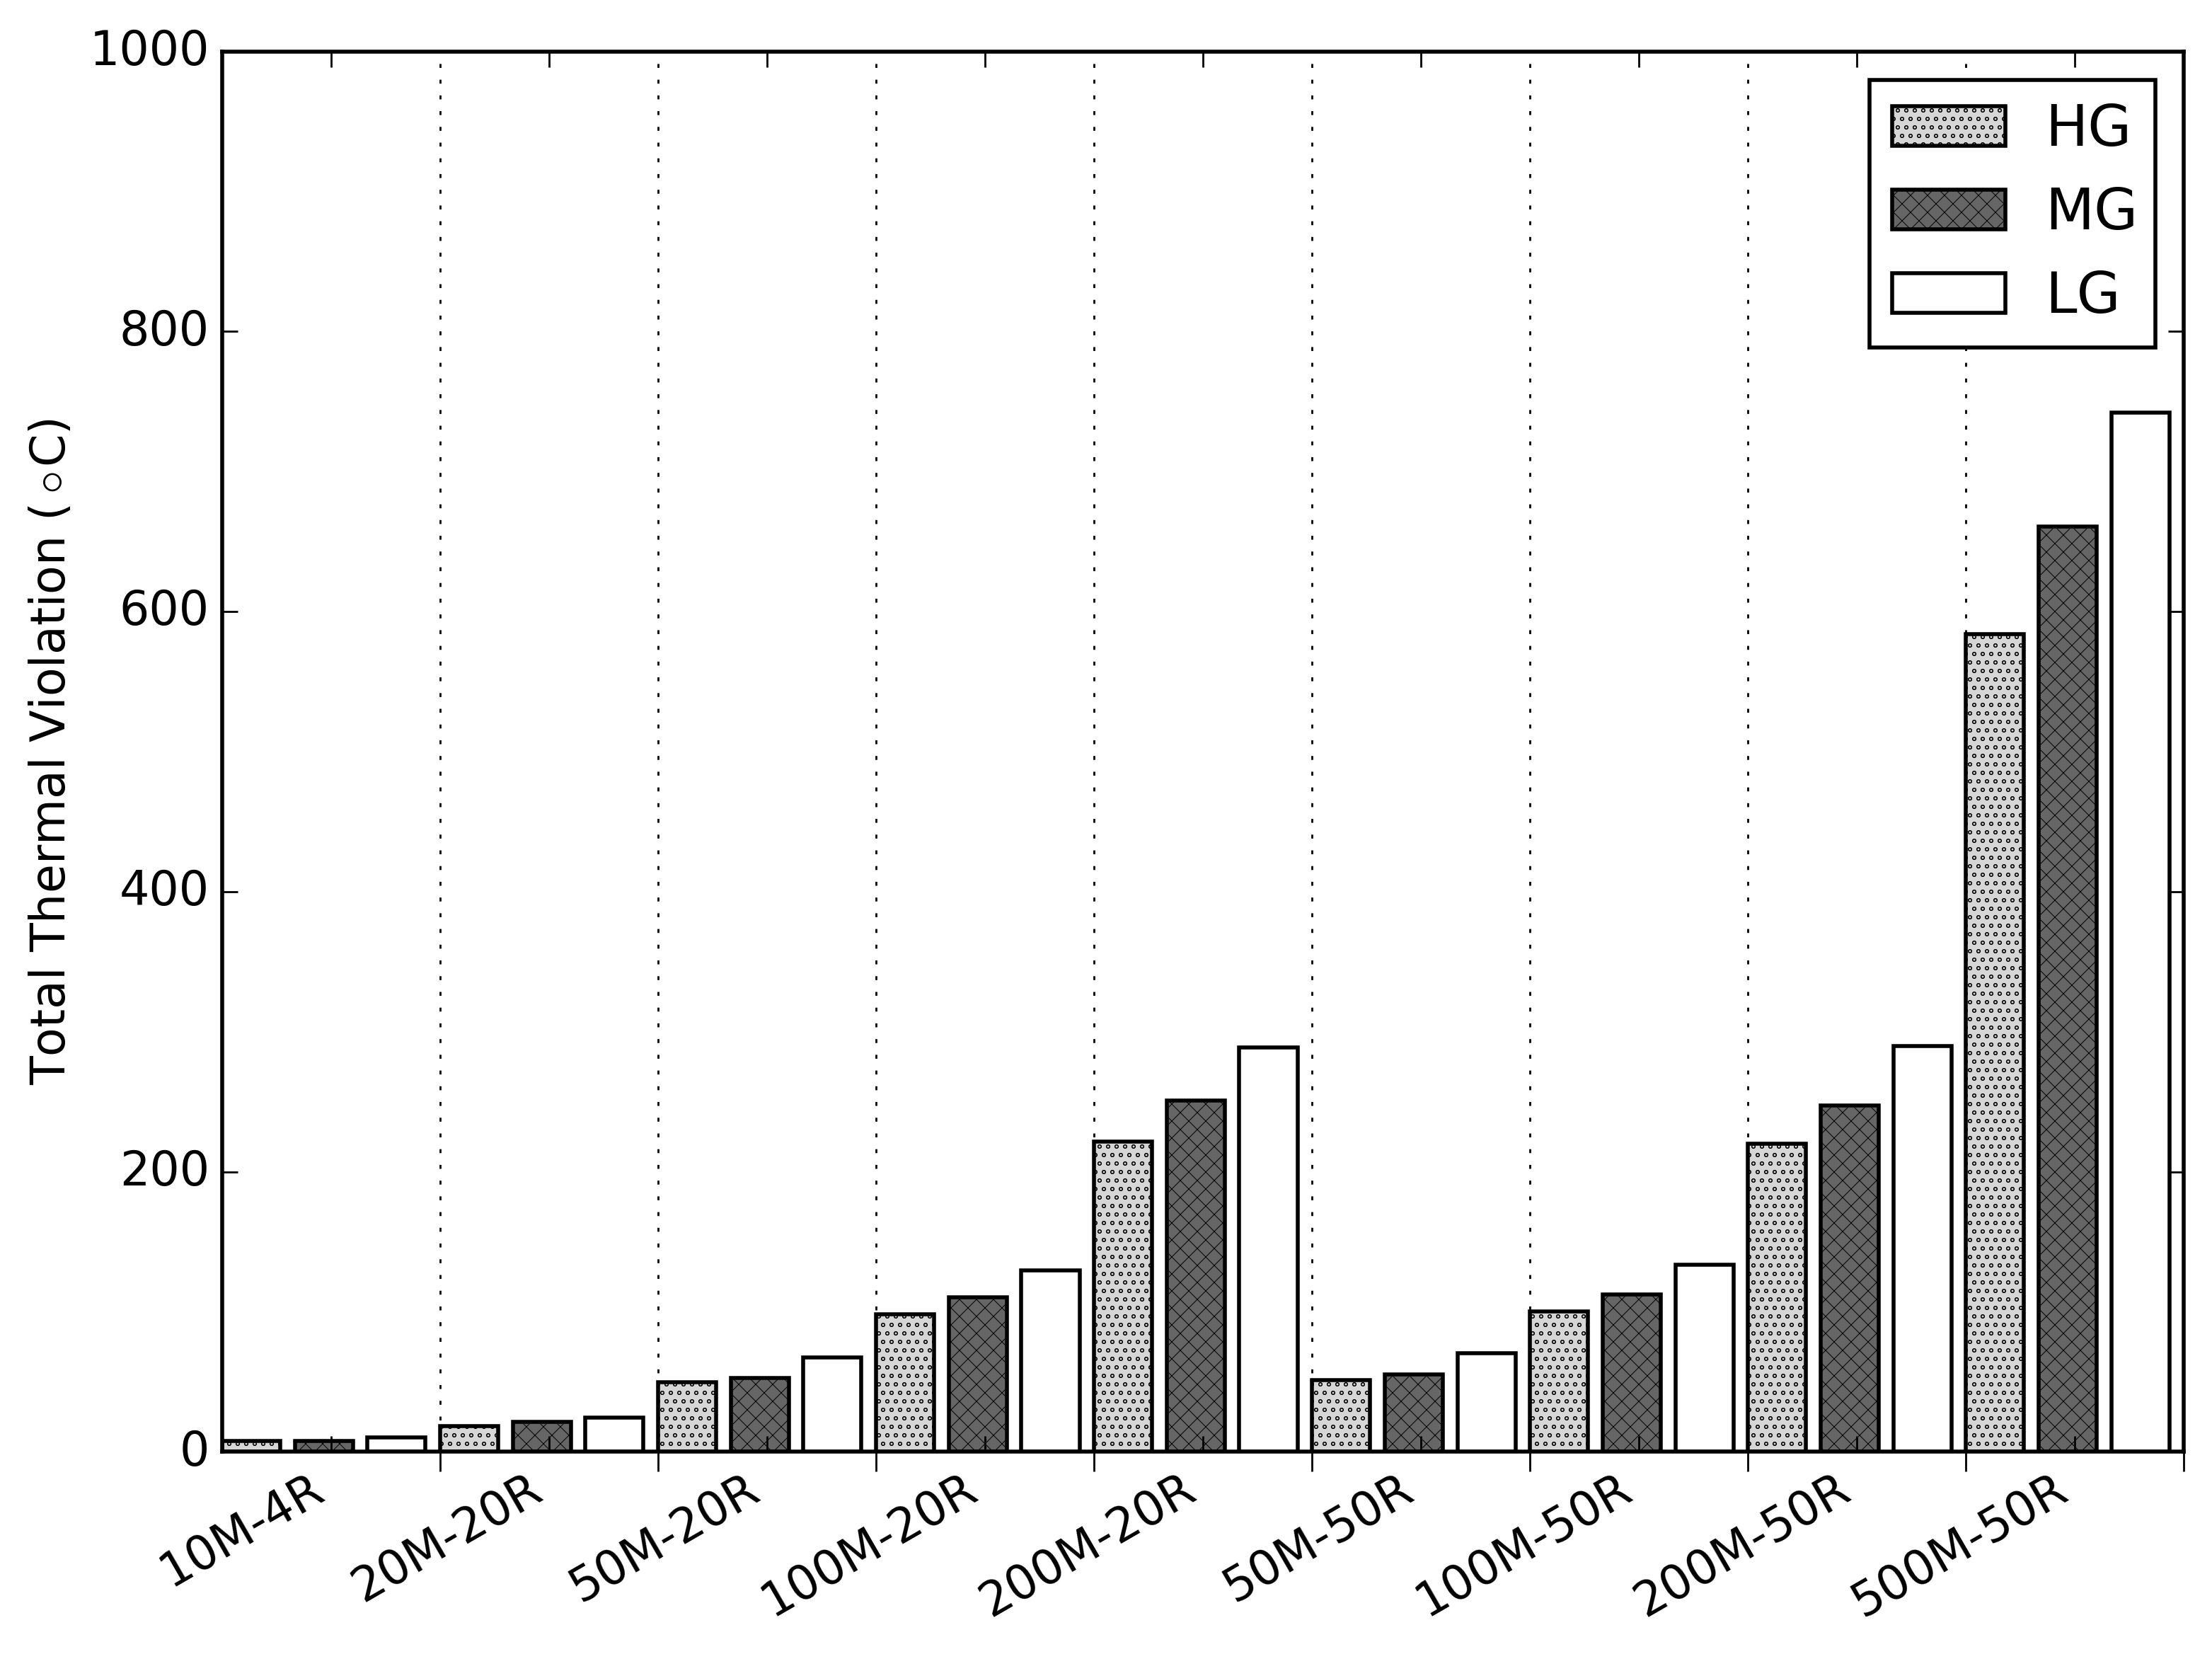
\includegraphics[width=0.6\linewidth]{figs/total_thermal_violation_diff_temp_flex_def_vs_oarb_oat.png} \\
(c) Total 
\end{tabular}
\caption{Effects to thermal comfort with adaptive temperature control - OATA approach}
\label{fig:atc_ot}
\end{figure}

\begin{figure}
\centering
\begin{tabular}{c}
  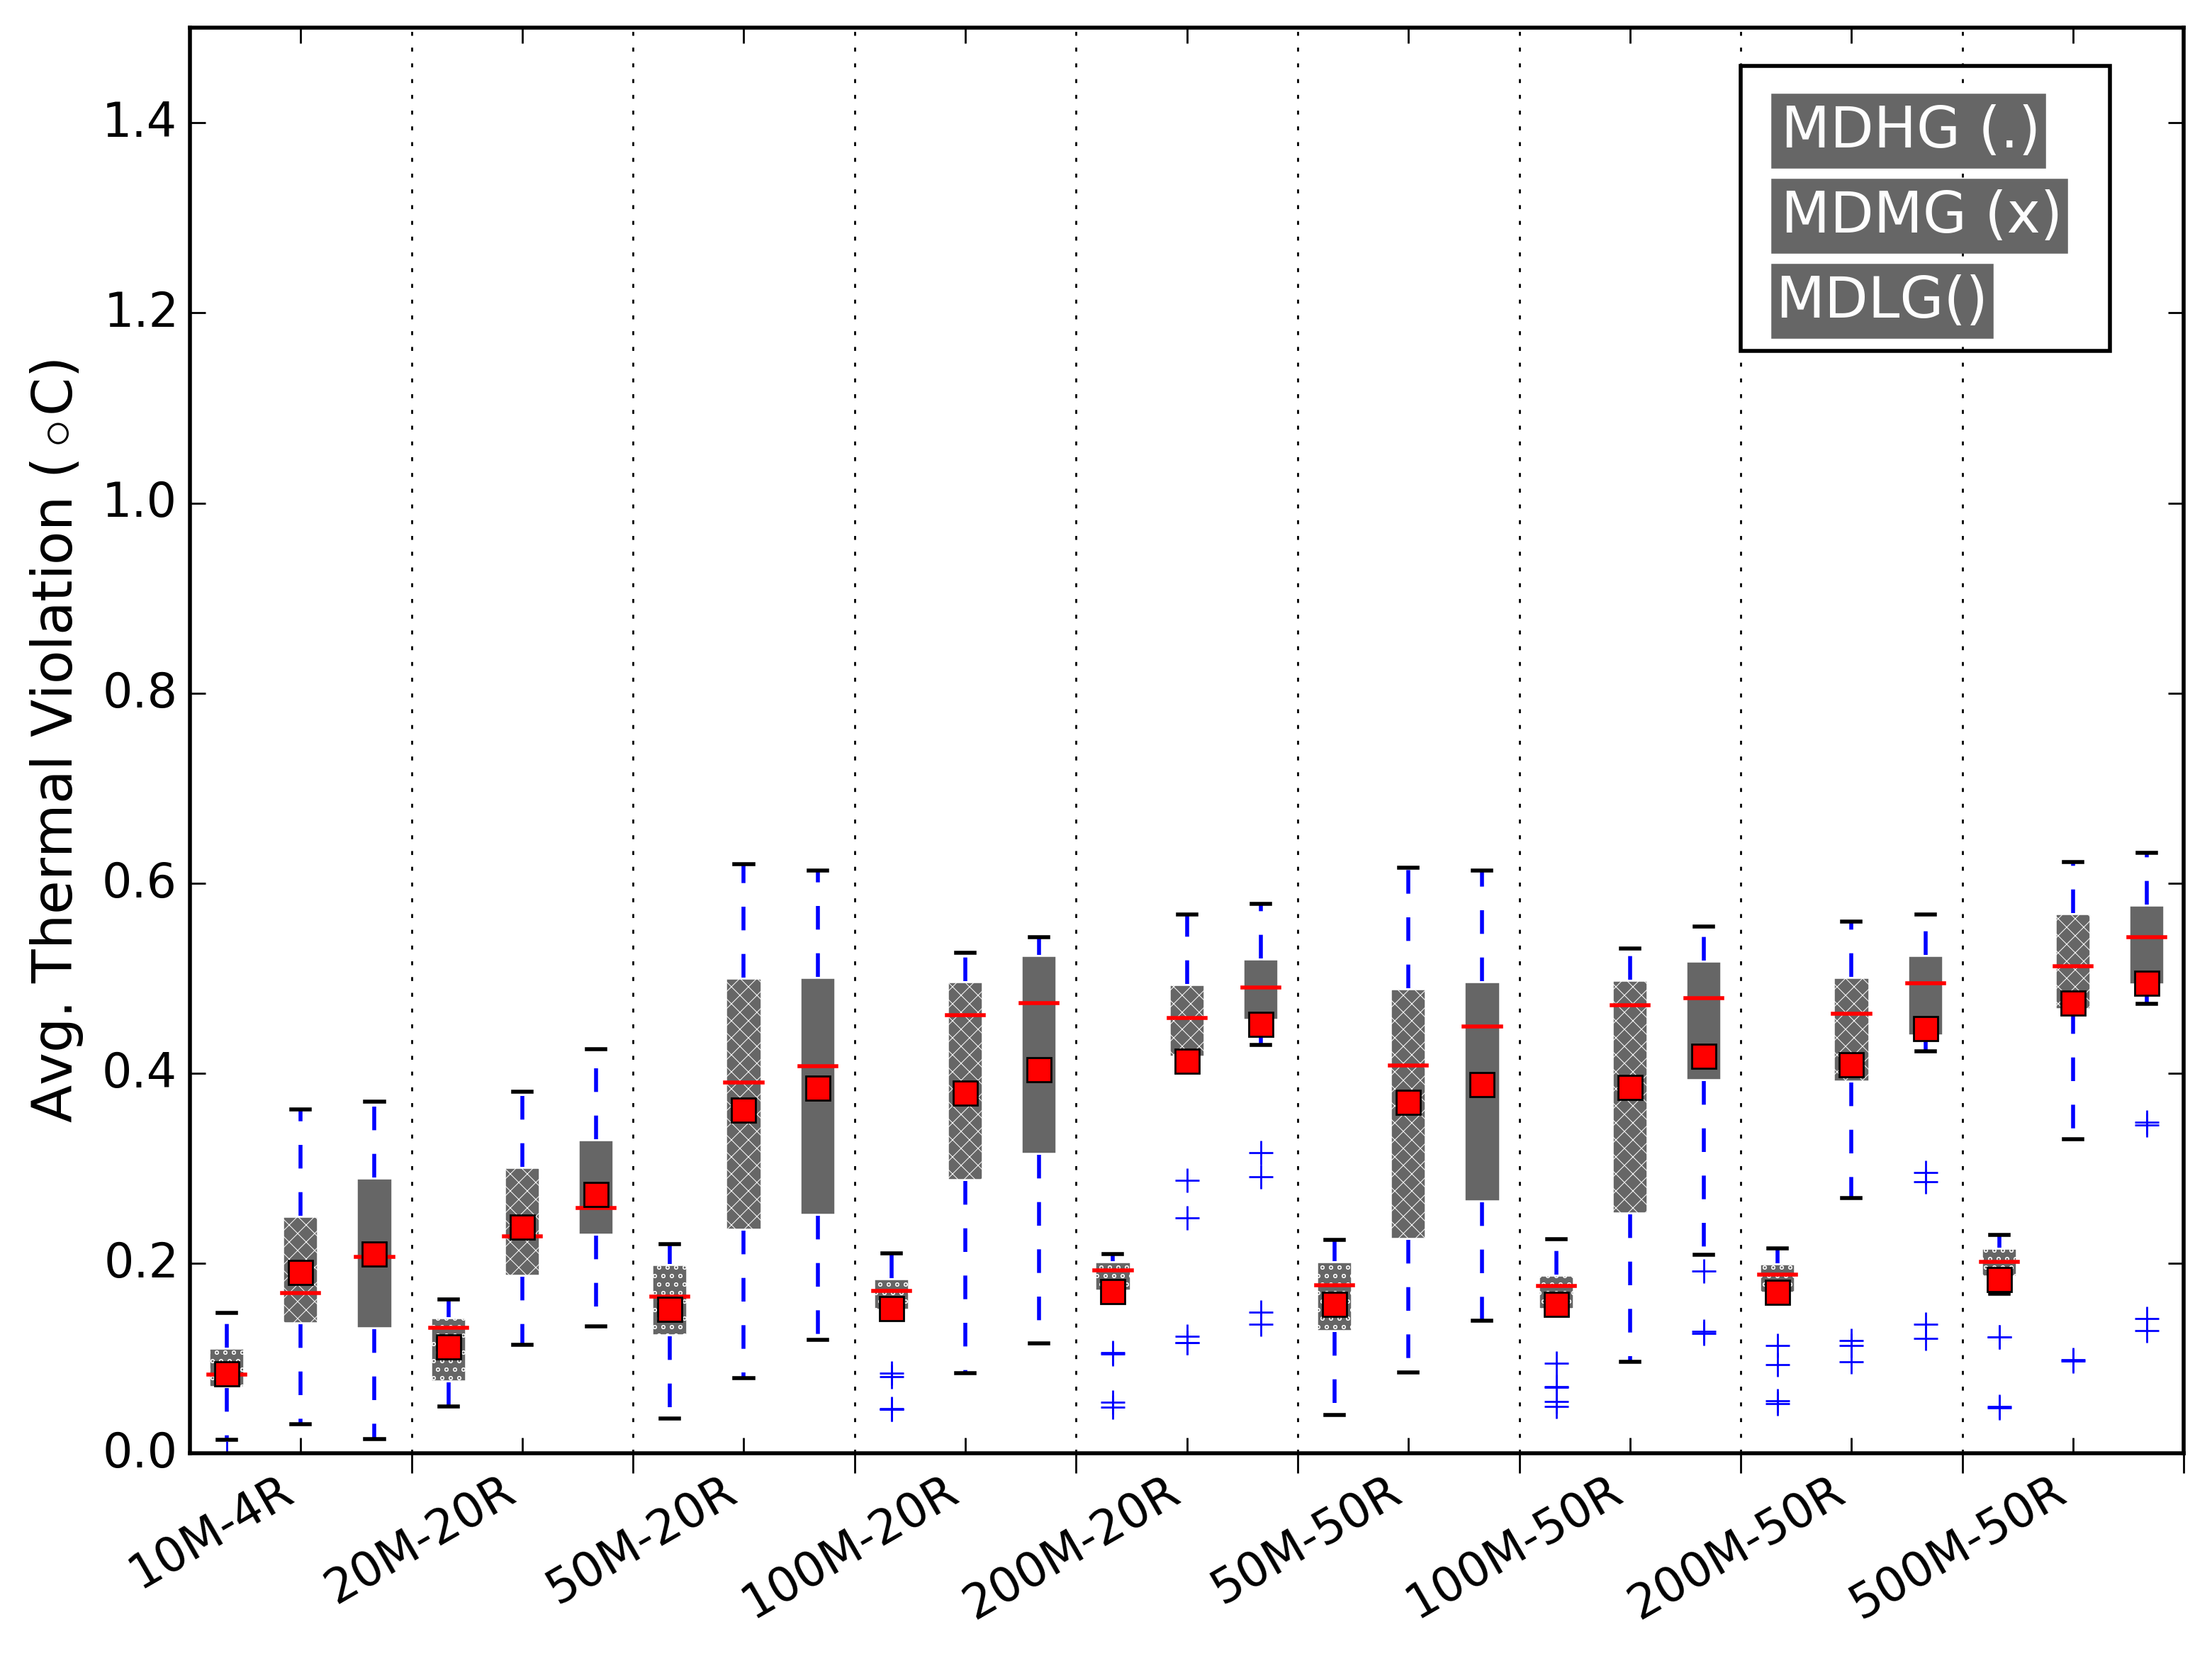
\includegraphics[width=0.9\linewidth]{figs/avg_thermal_violation_diff_temp_flex_def_vs_oarb_medium_boxplot_mtd.png} \\
(a) MD \\[6pt]
  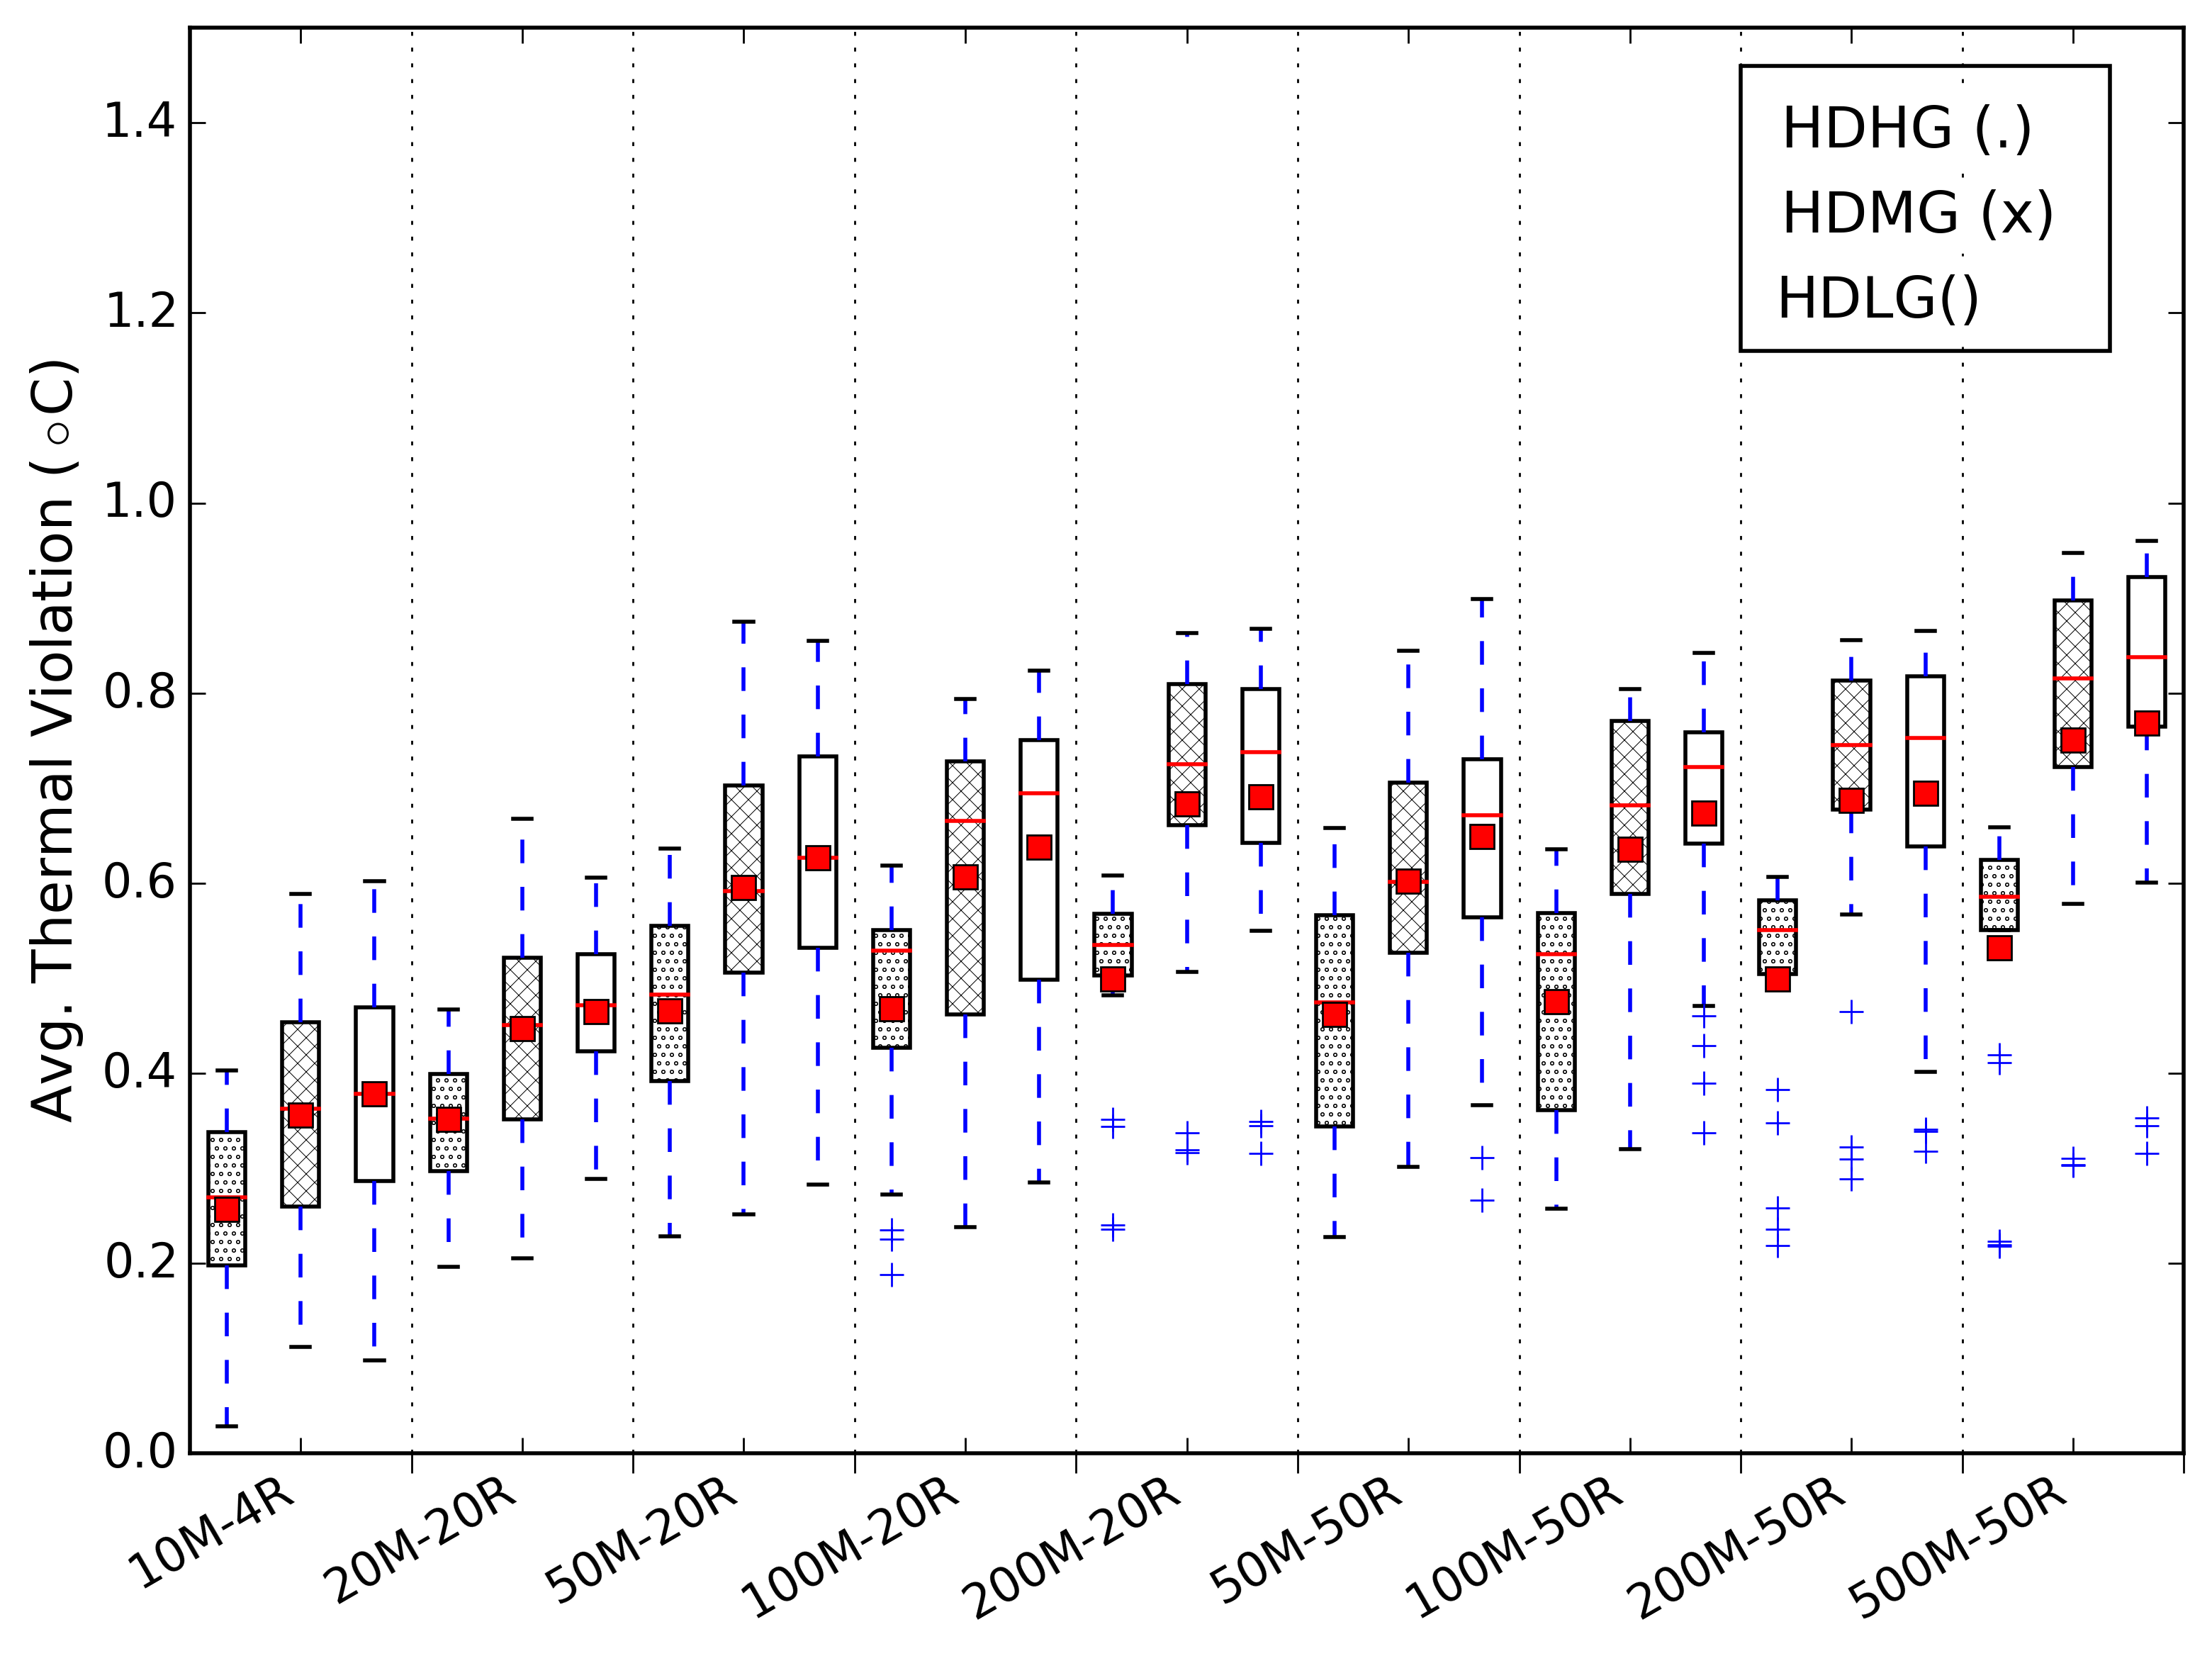
\includegraphics[width=0.9\linewidth]{figs/avg_thermal_violation_diff_temp_flex_def_vs_oarb_high_boxplot_mtd.png} \\
(b) HD \\[6pt]	
\end{tabular}
\caption{MTDA approach - temperature deviation vs robustness to thermal comfort}
\label{fig:atc_mtrb}
\end{figure}

%\begin{figure}
%\centering
%\begin{tabular}{c}
  %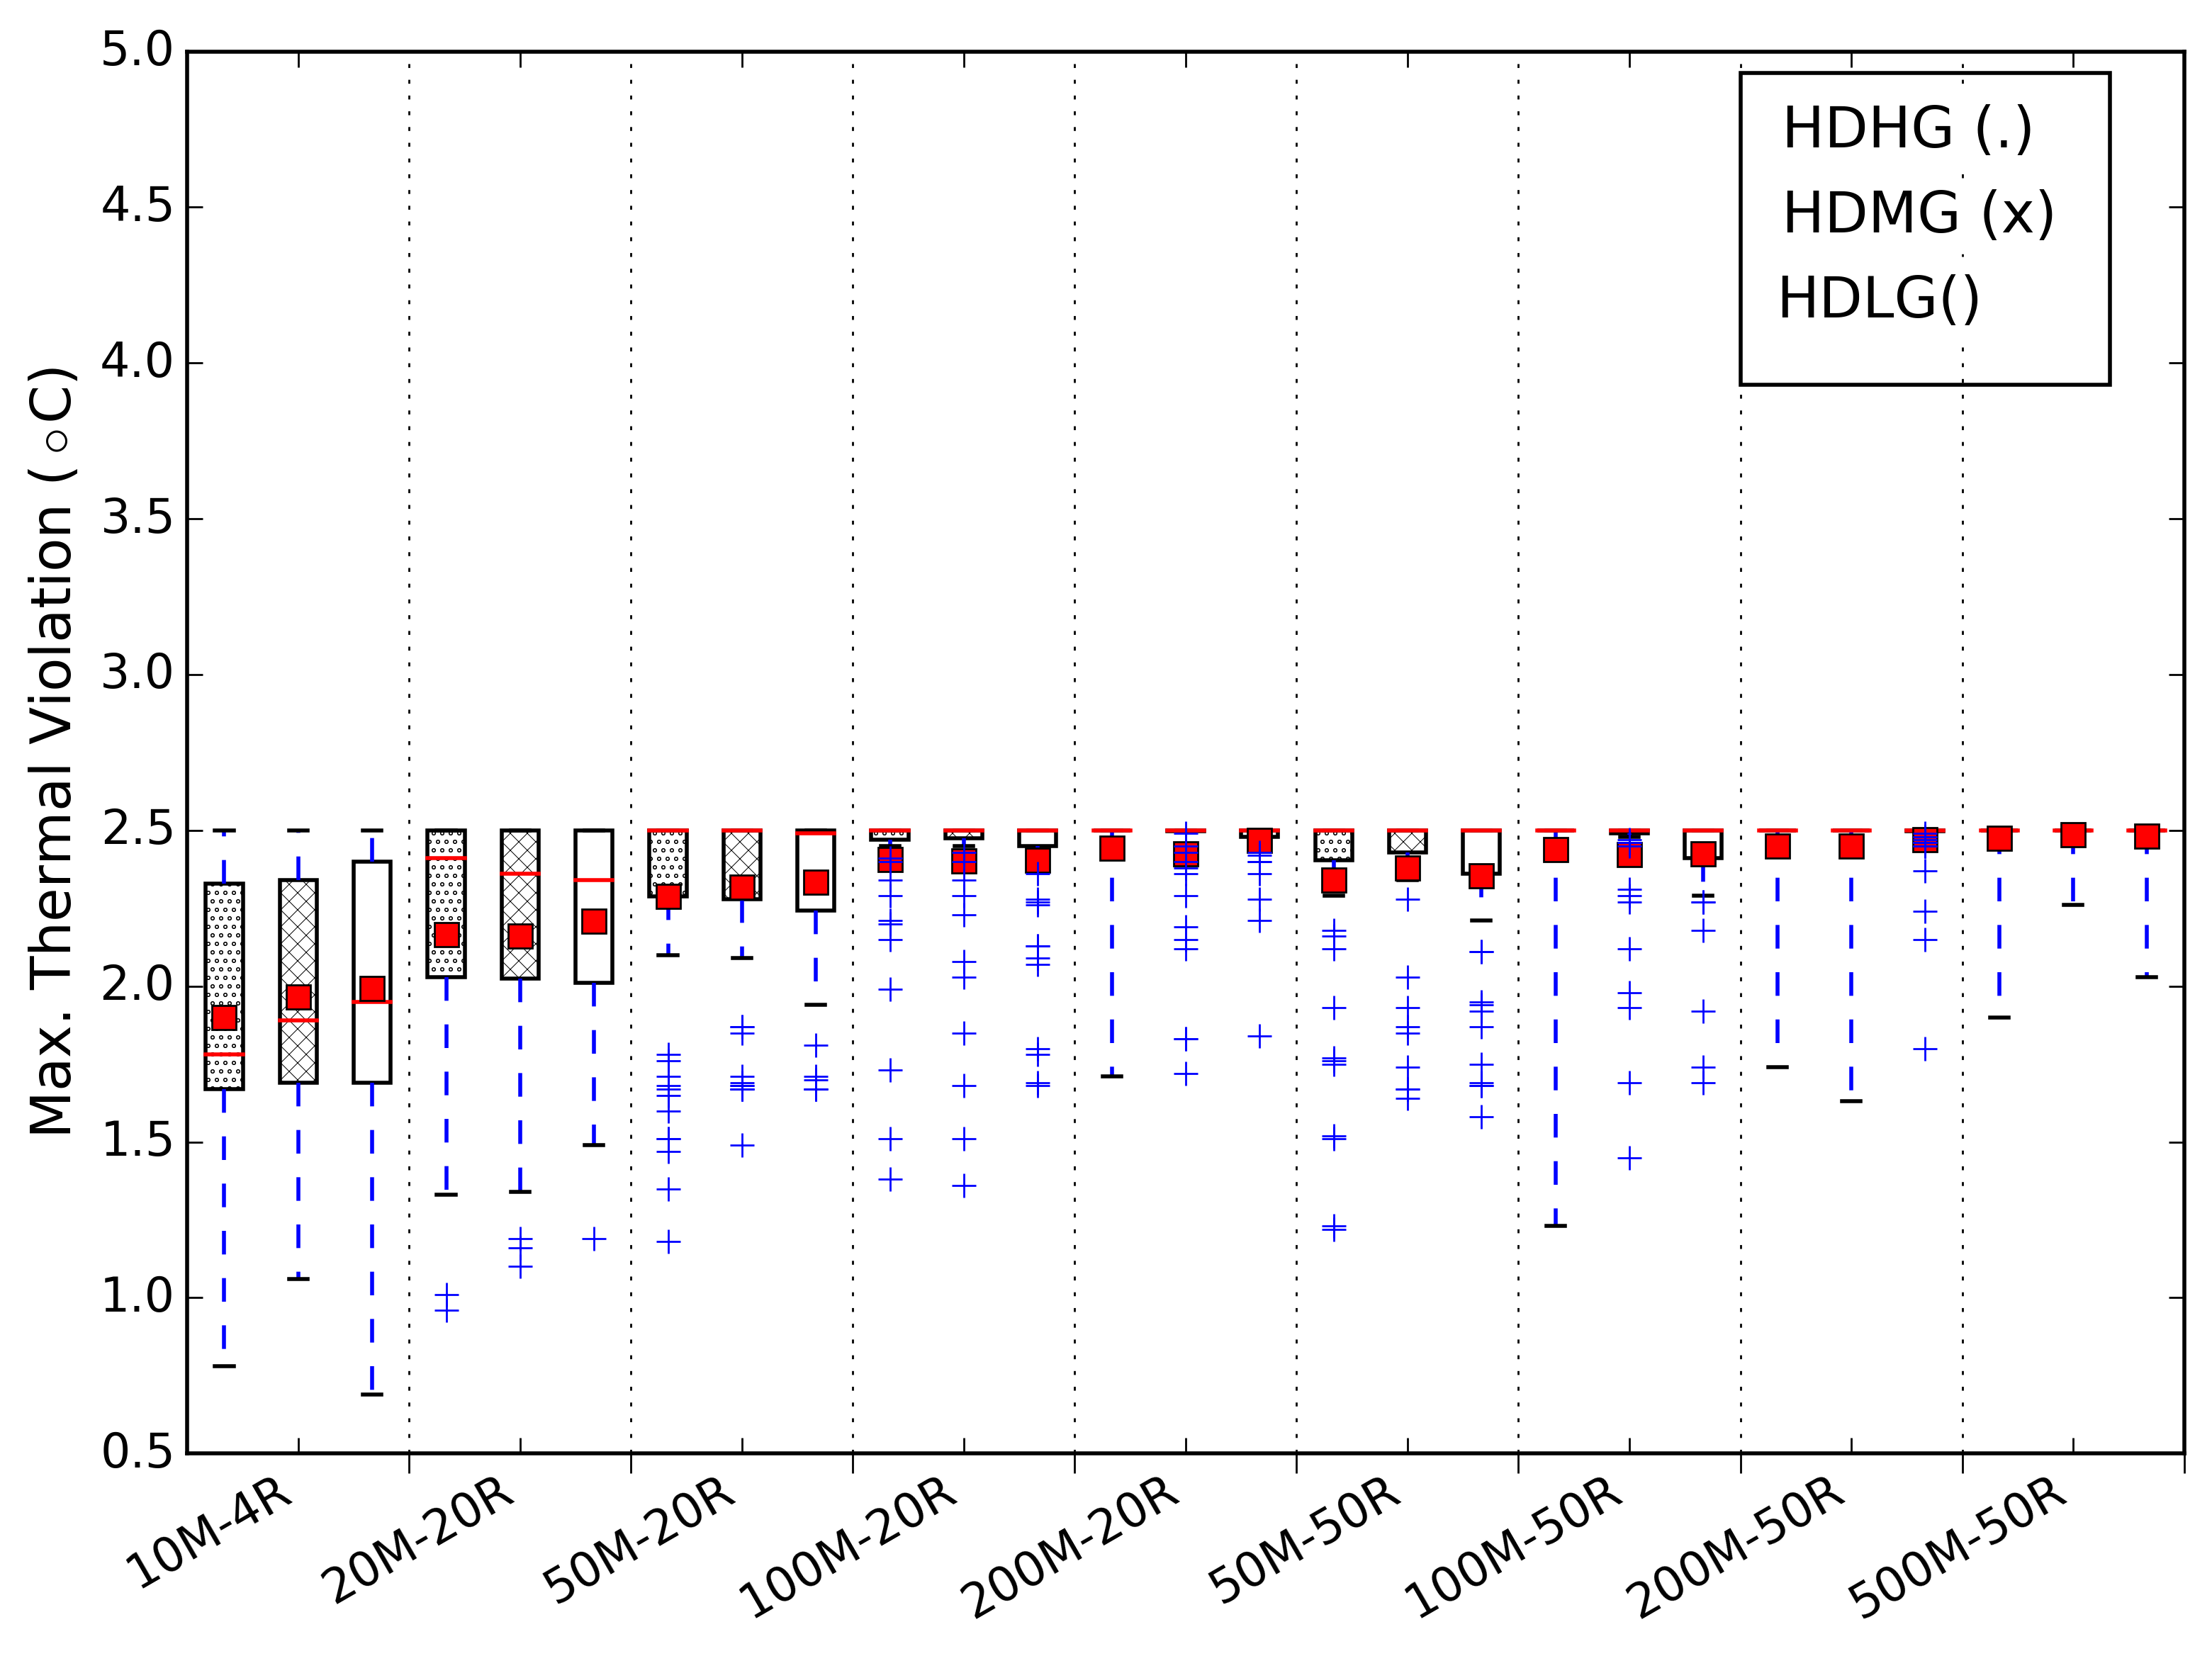
\includegraphics[width=0.6\linewidth]{figs/max_thermal_violation_diff_temp_flex_def_vs_oarb_high_boxplot_mtd.png} \\
%(a) Maximum \\[6pt]
  %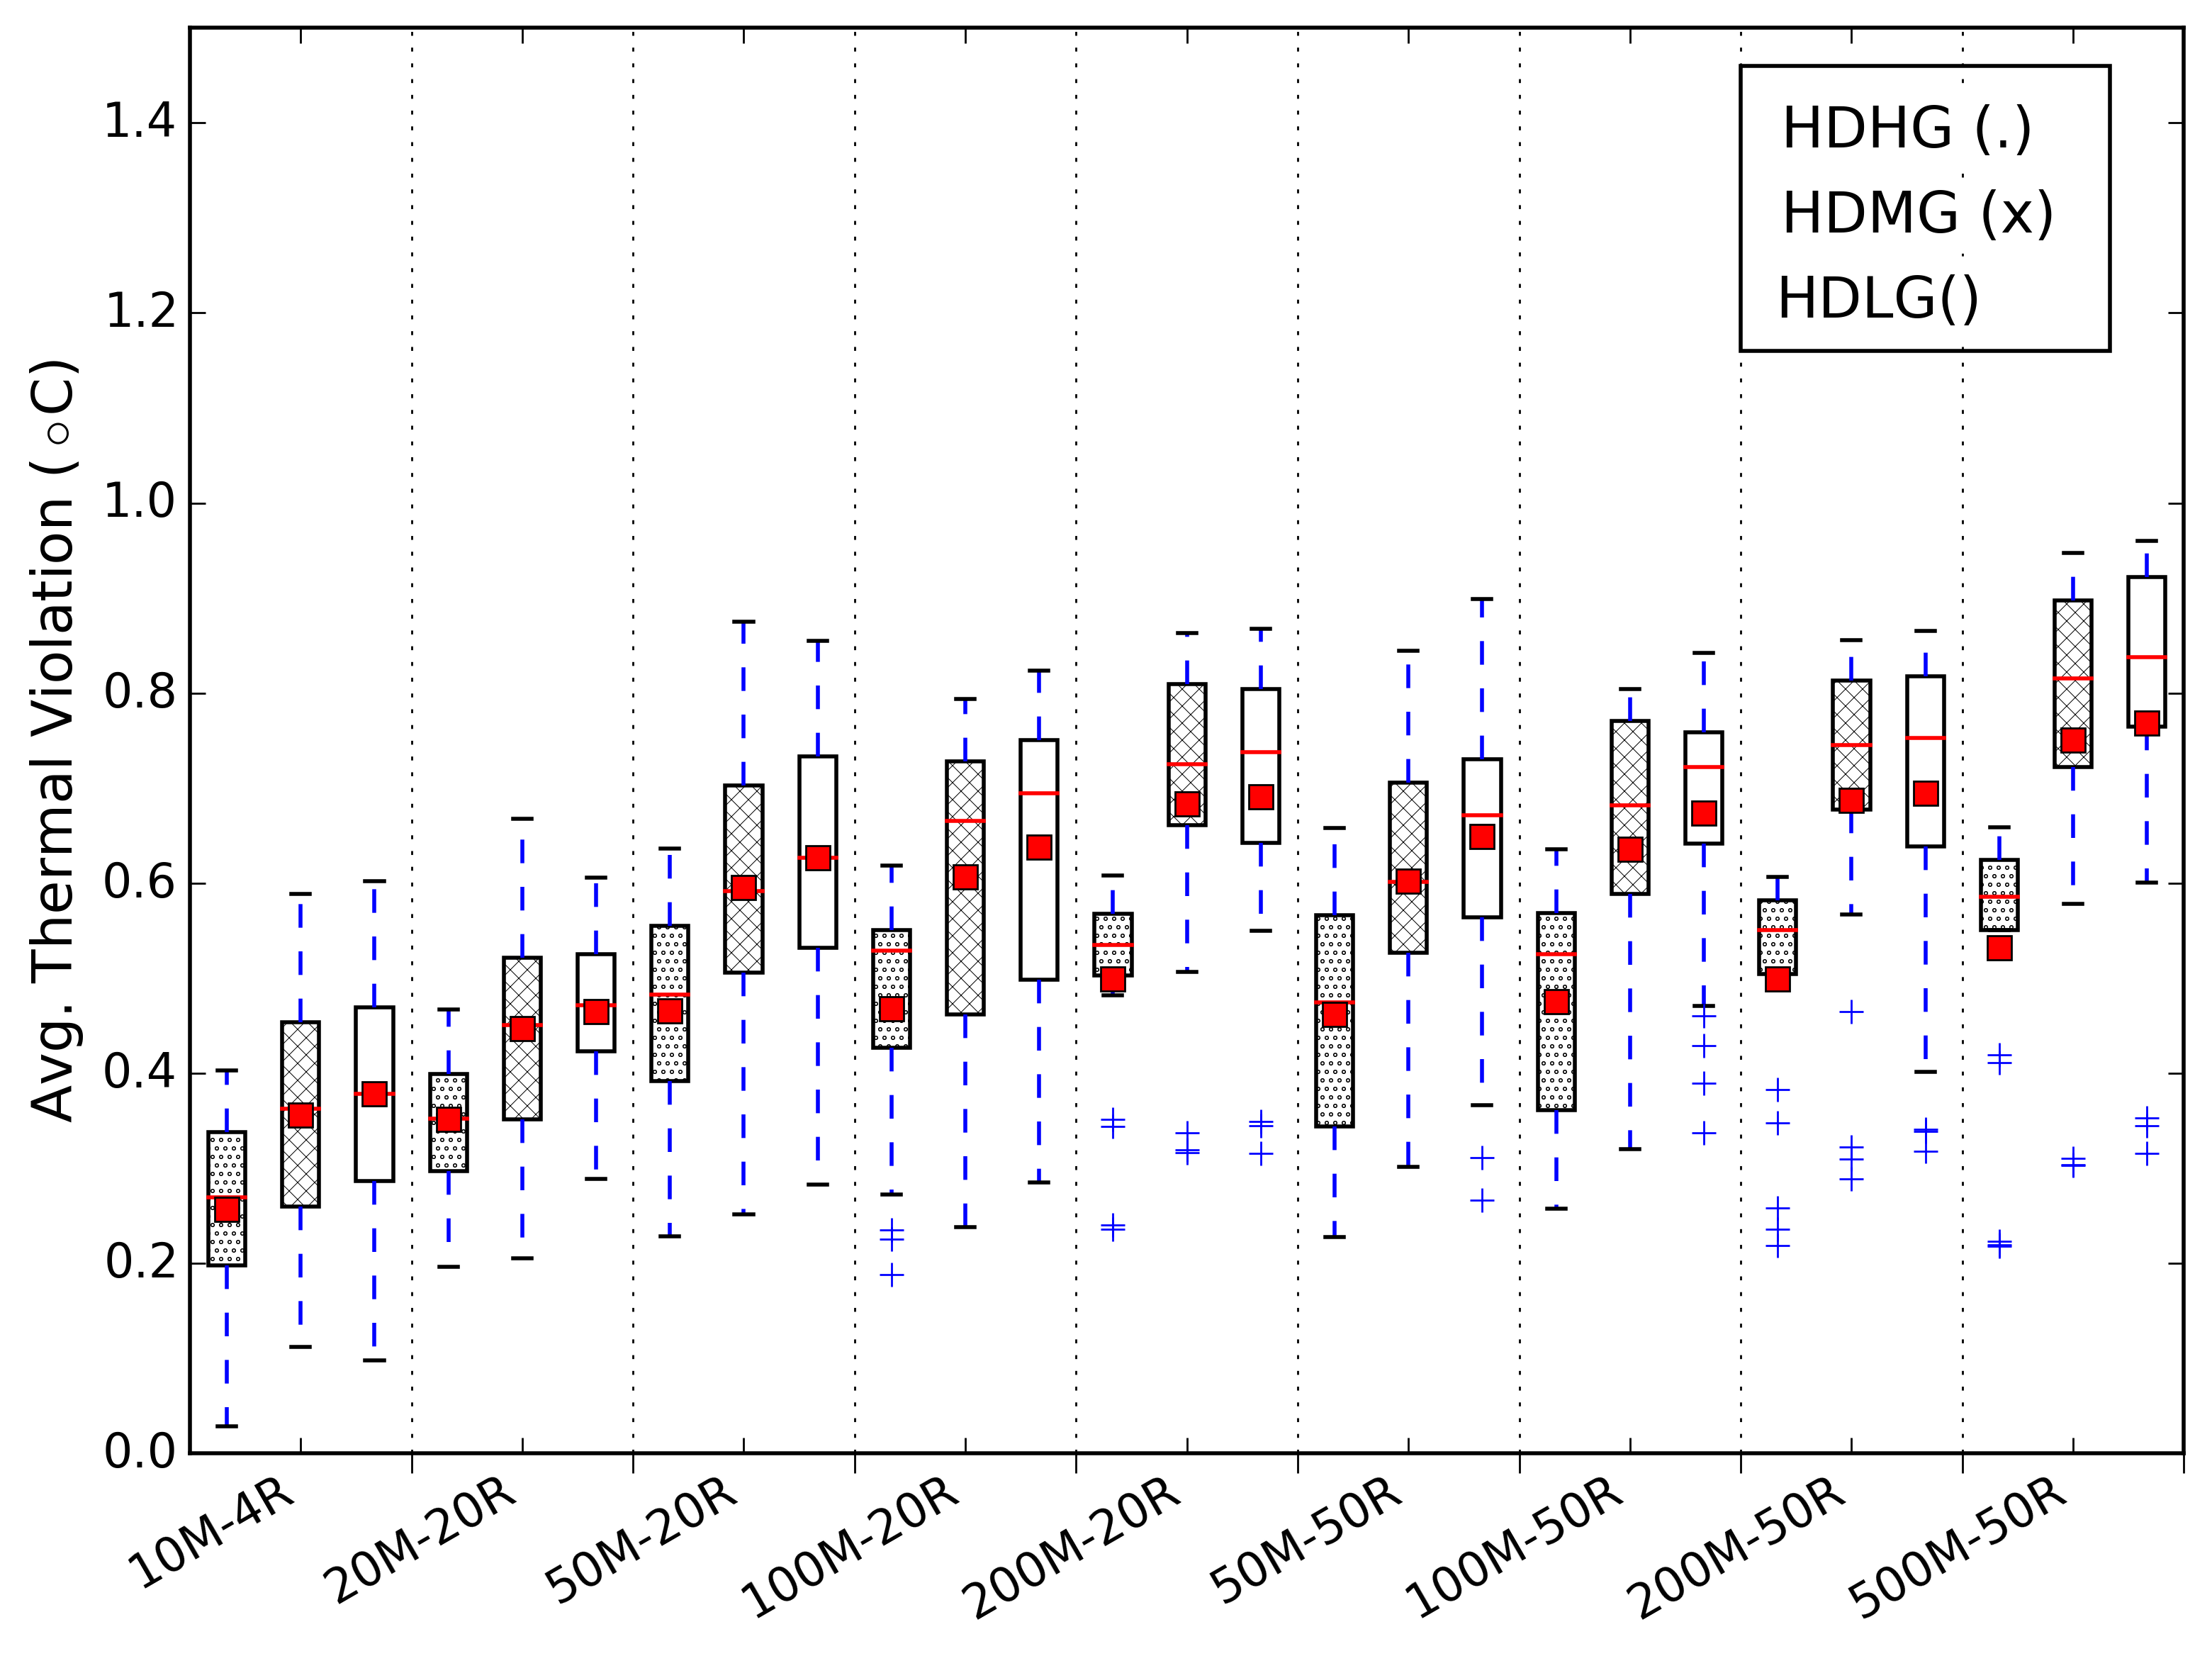
\includegraphics[width=0.6\linewidth]{figs/avg_thermal_violation_diff_temp_flex_def_vs_oarb_high_boxplot_mtd.png} \\
%(b) Average \\[6pt]
	%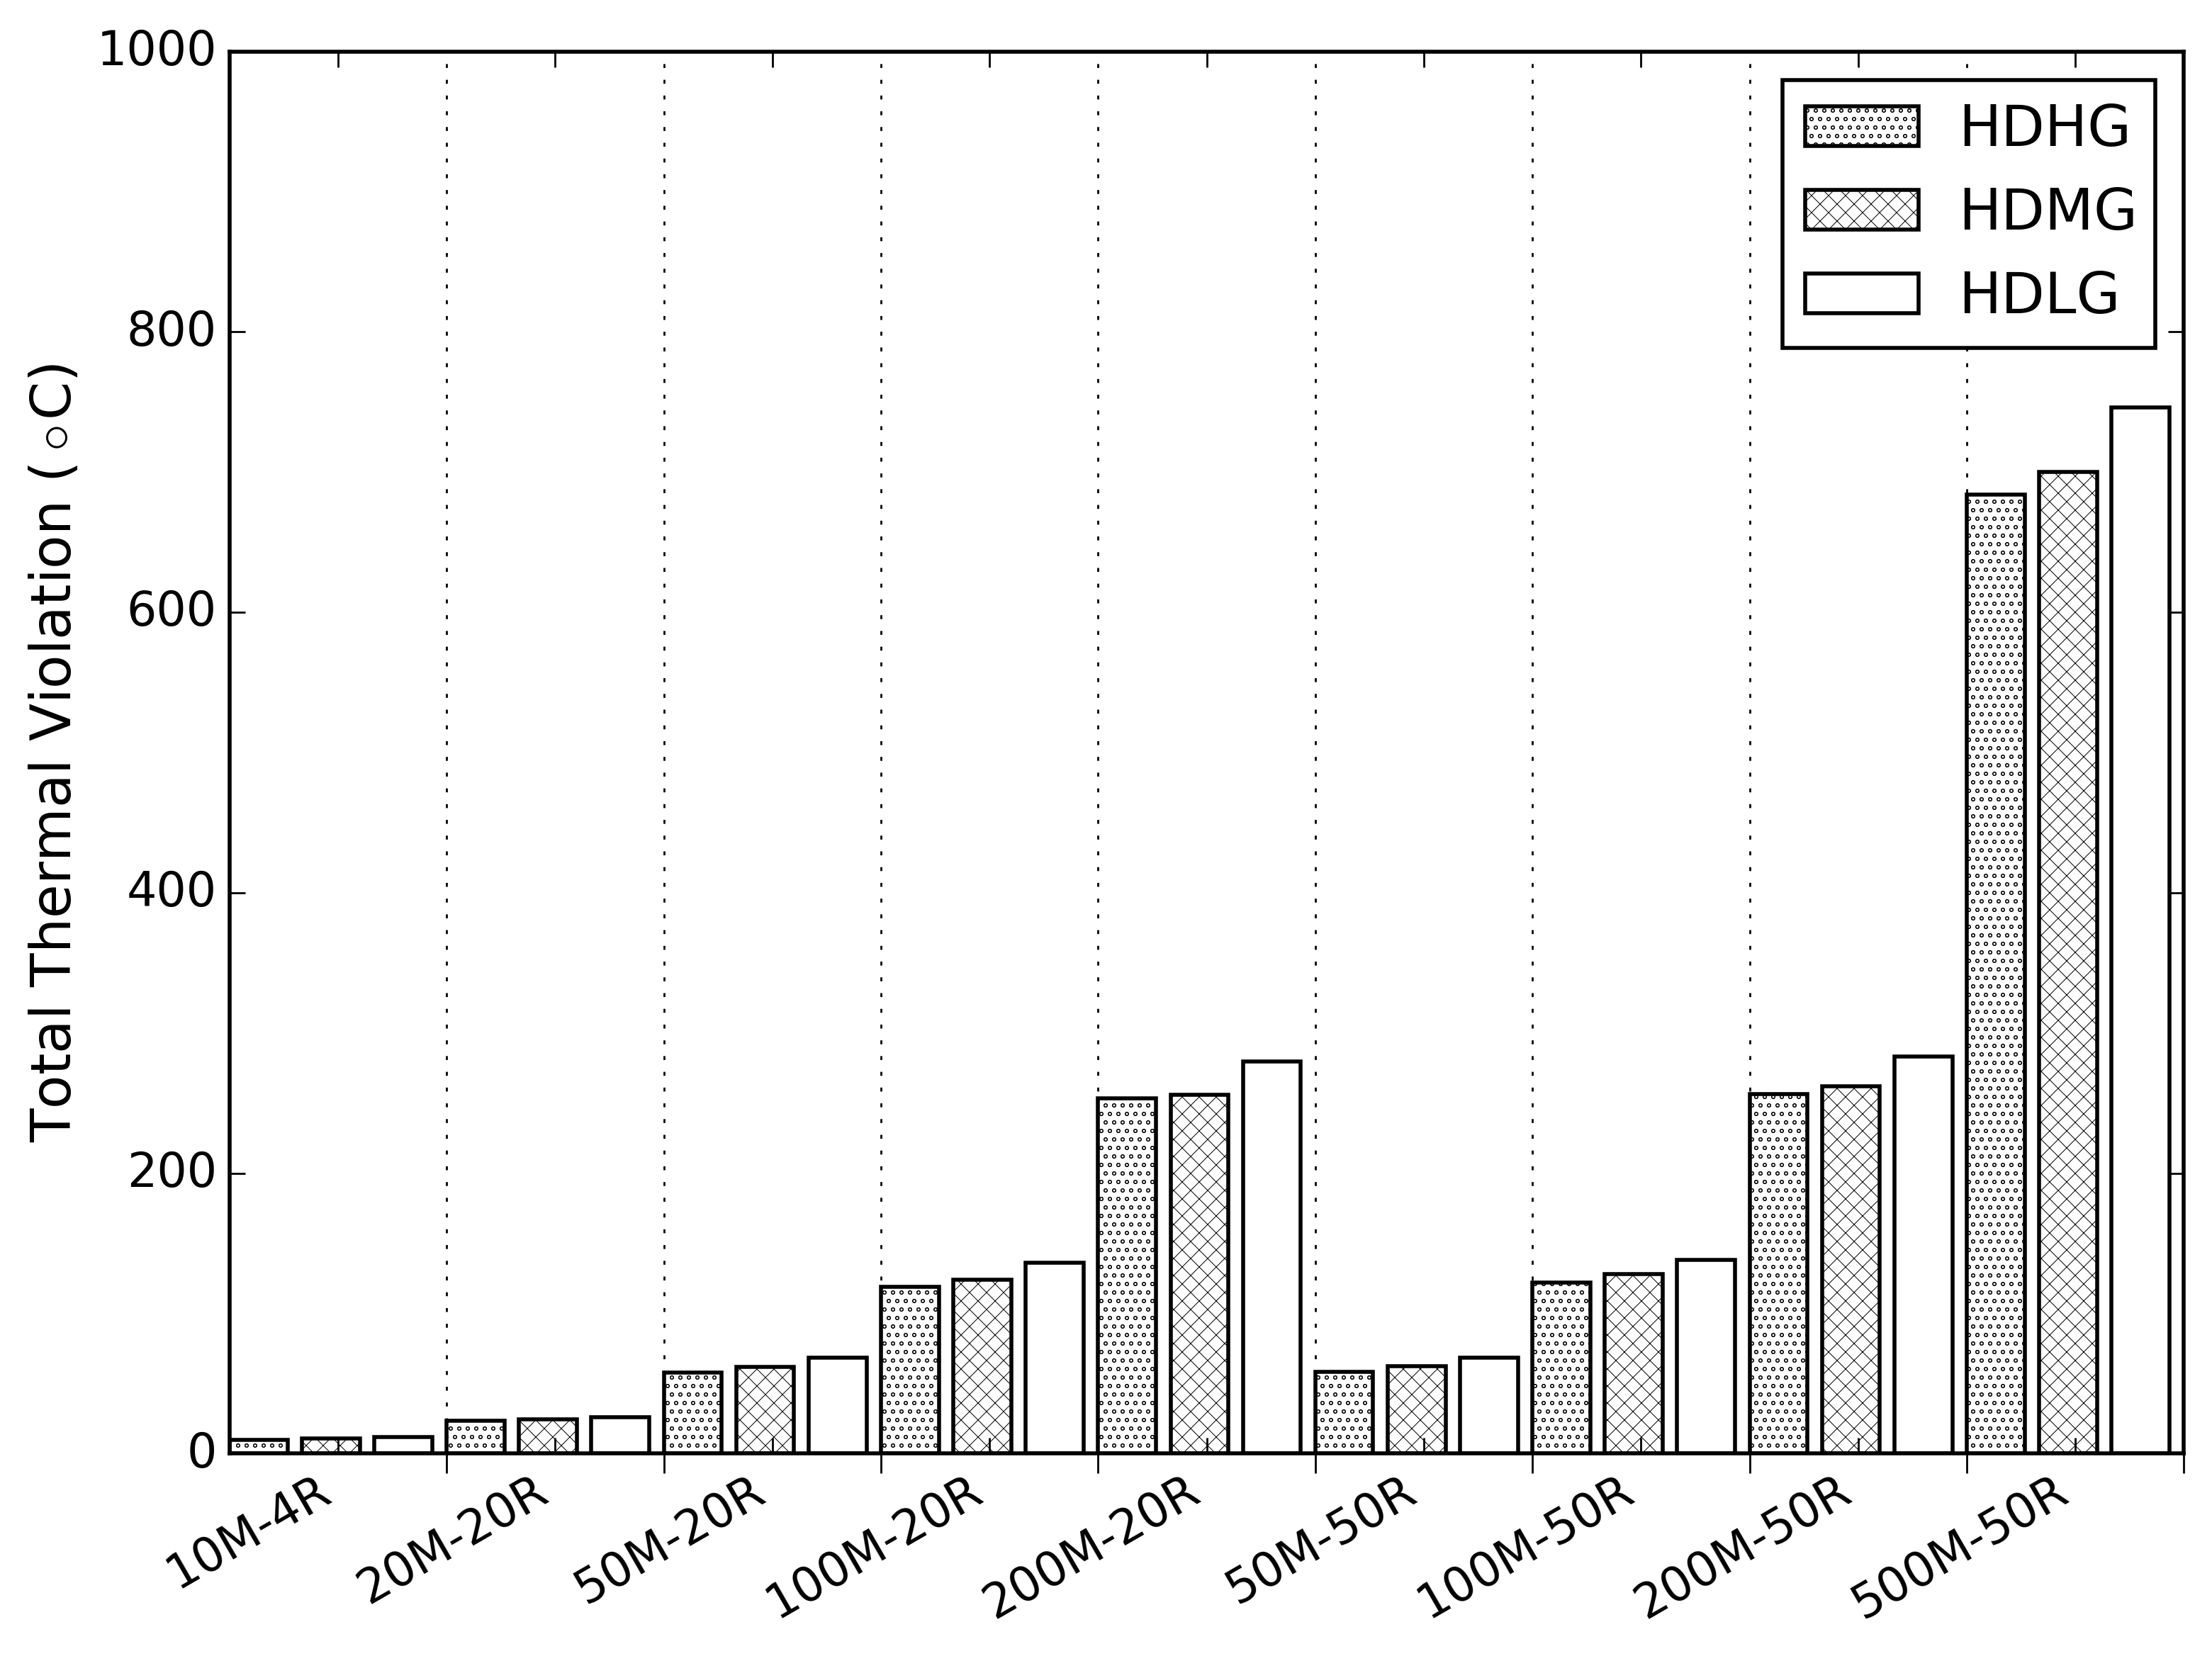
\includegraphics[width=0.6\linewidth]{figs/total_thermal_violation_diff_temp_flex_def_vs_oarb_high_mtd.png} \\
%(c) Total 
%\end{tabular}
%\caption{MTDA approach - Temperature Deviation vs Robustness to Thermal Comfort (High Deviation)}
%\label{fig:atc_mthr}
%\end{figure}

%\begin{figure}
%\centering
%\begin{tabular}{c}
  %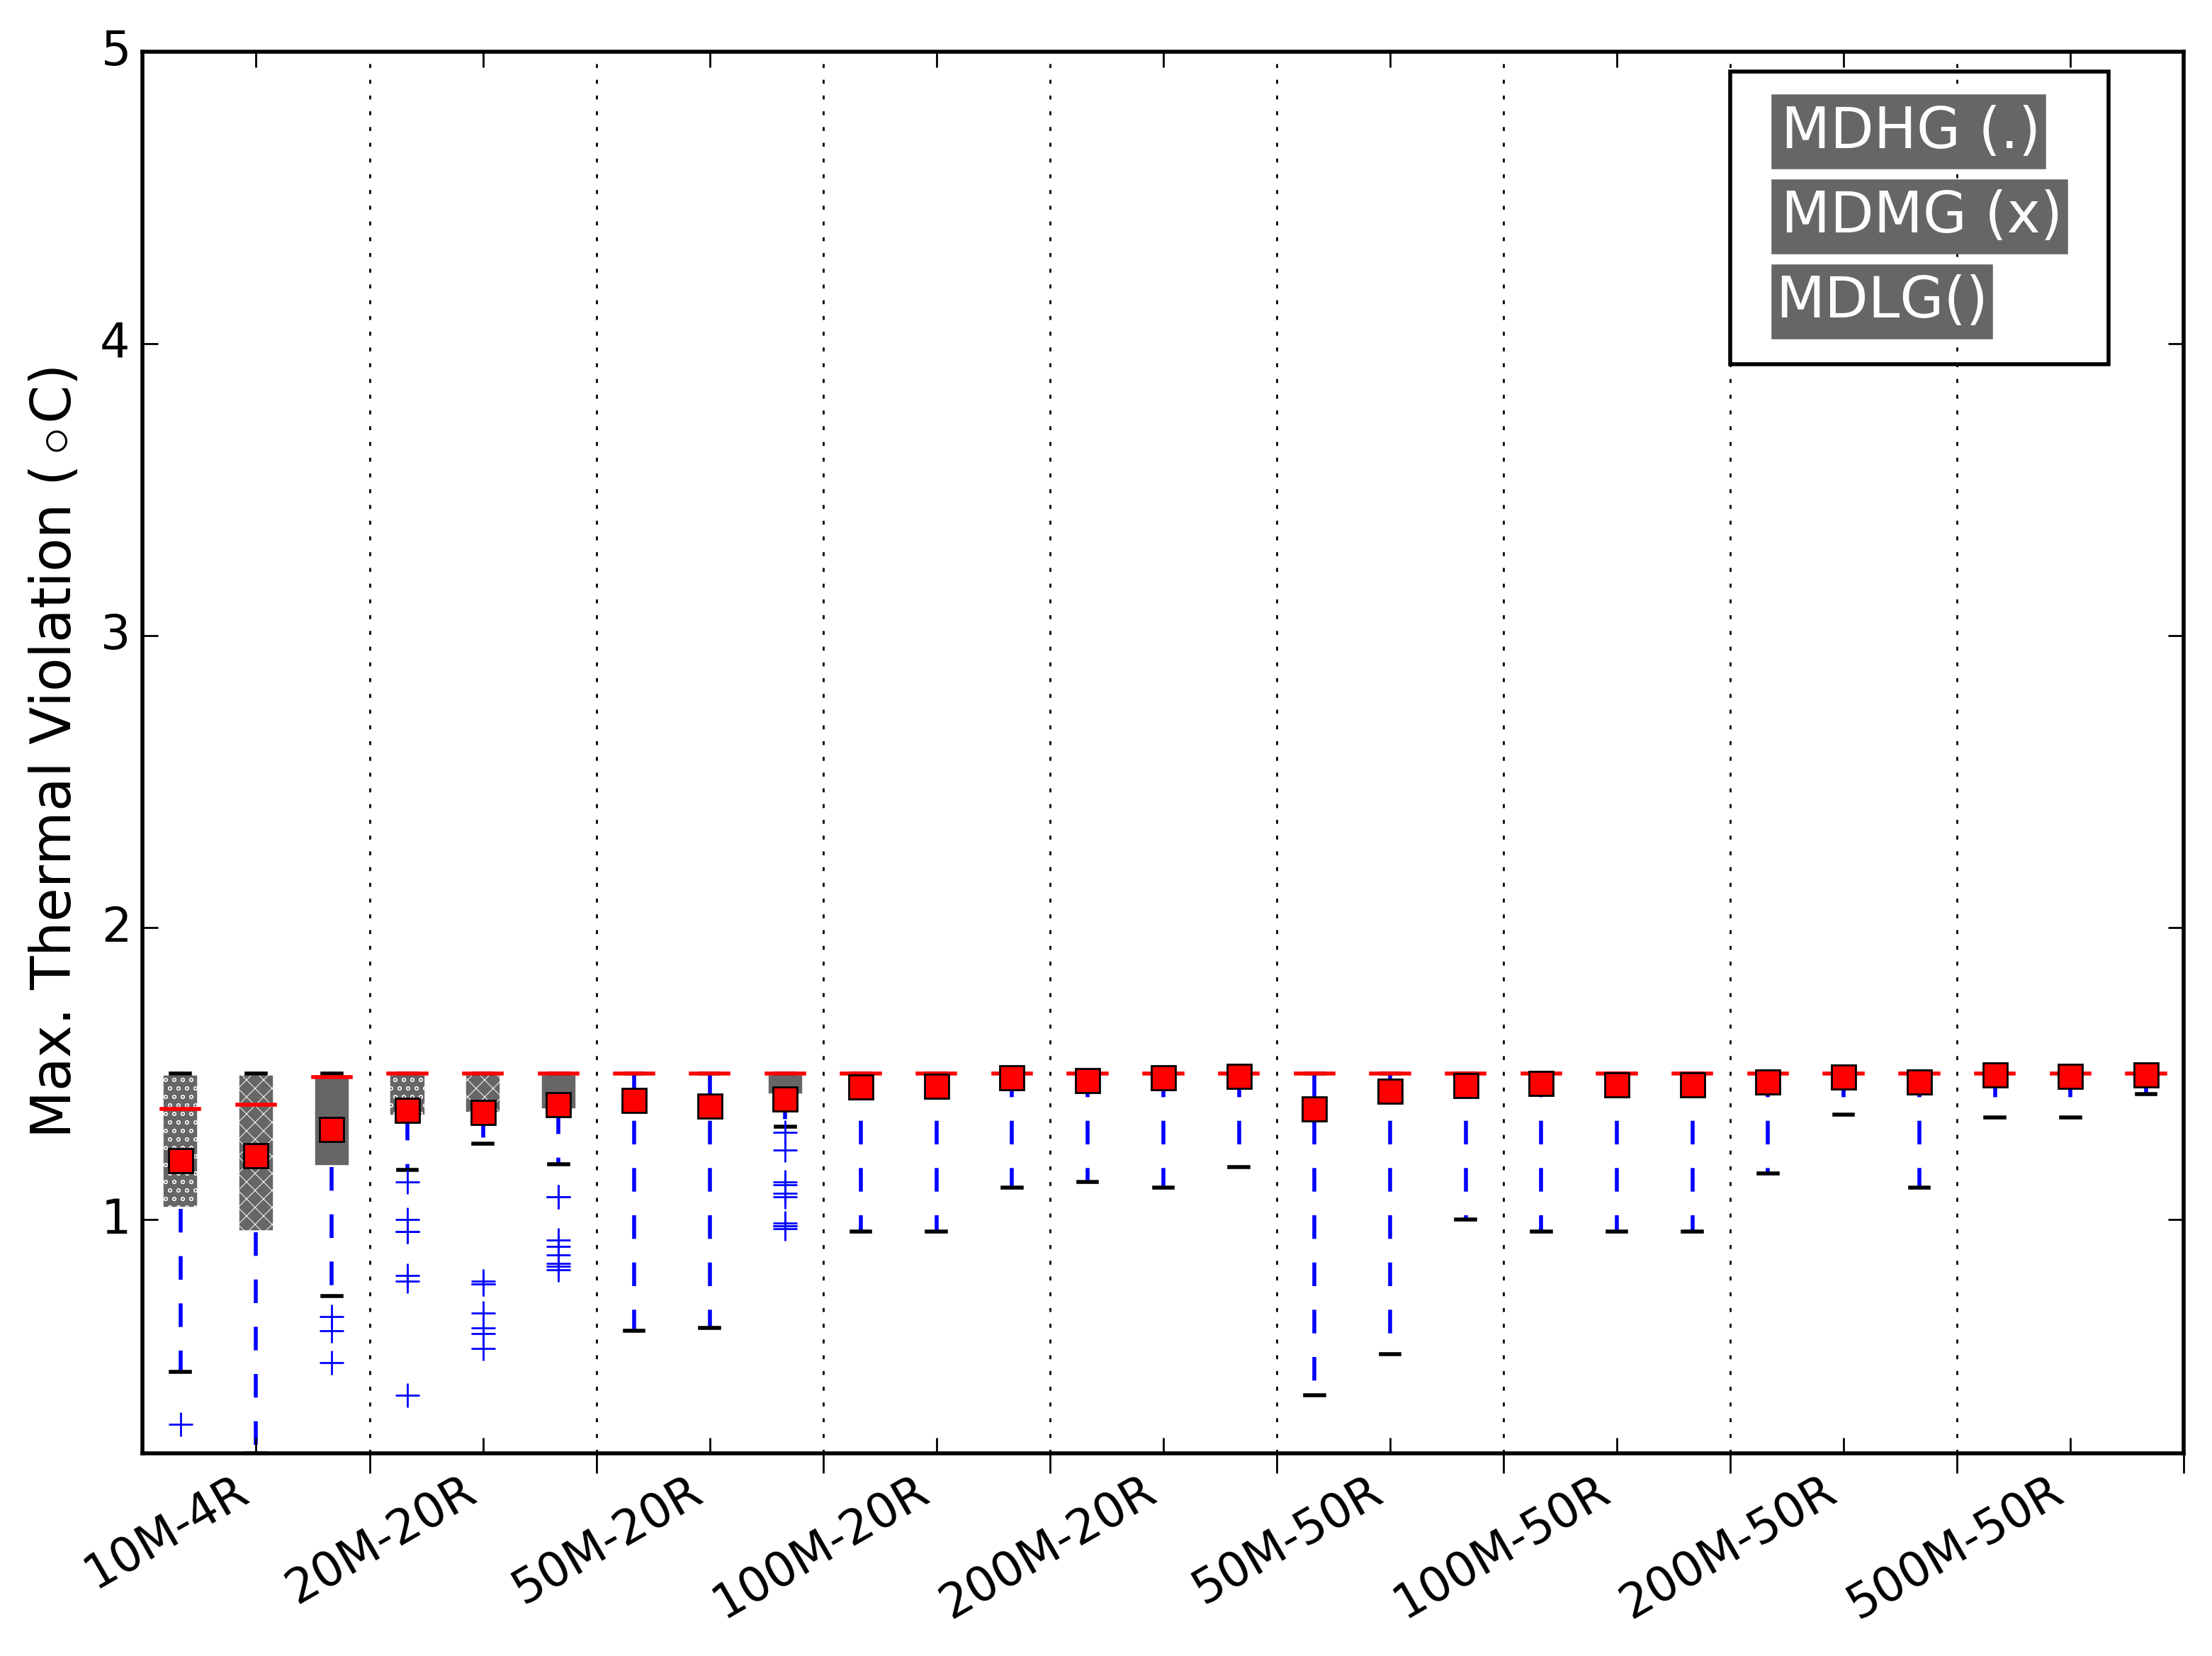
\includegraphics[width=0.6\linewidth]{figs/max_thermal_violation_diff_temp_flex_def_vs_oarb_medium_boxplot_mtd.png} \\
%(a) Maximum \\[6pt]
  %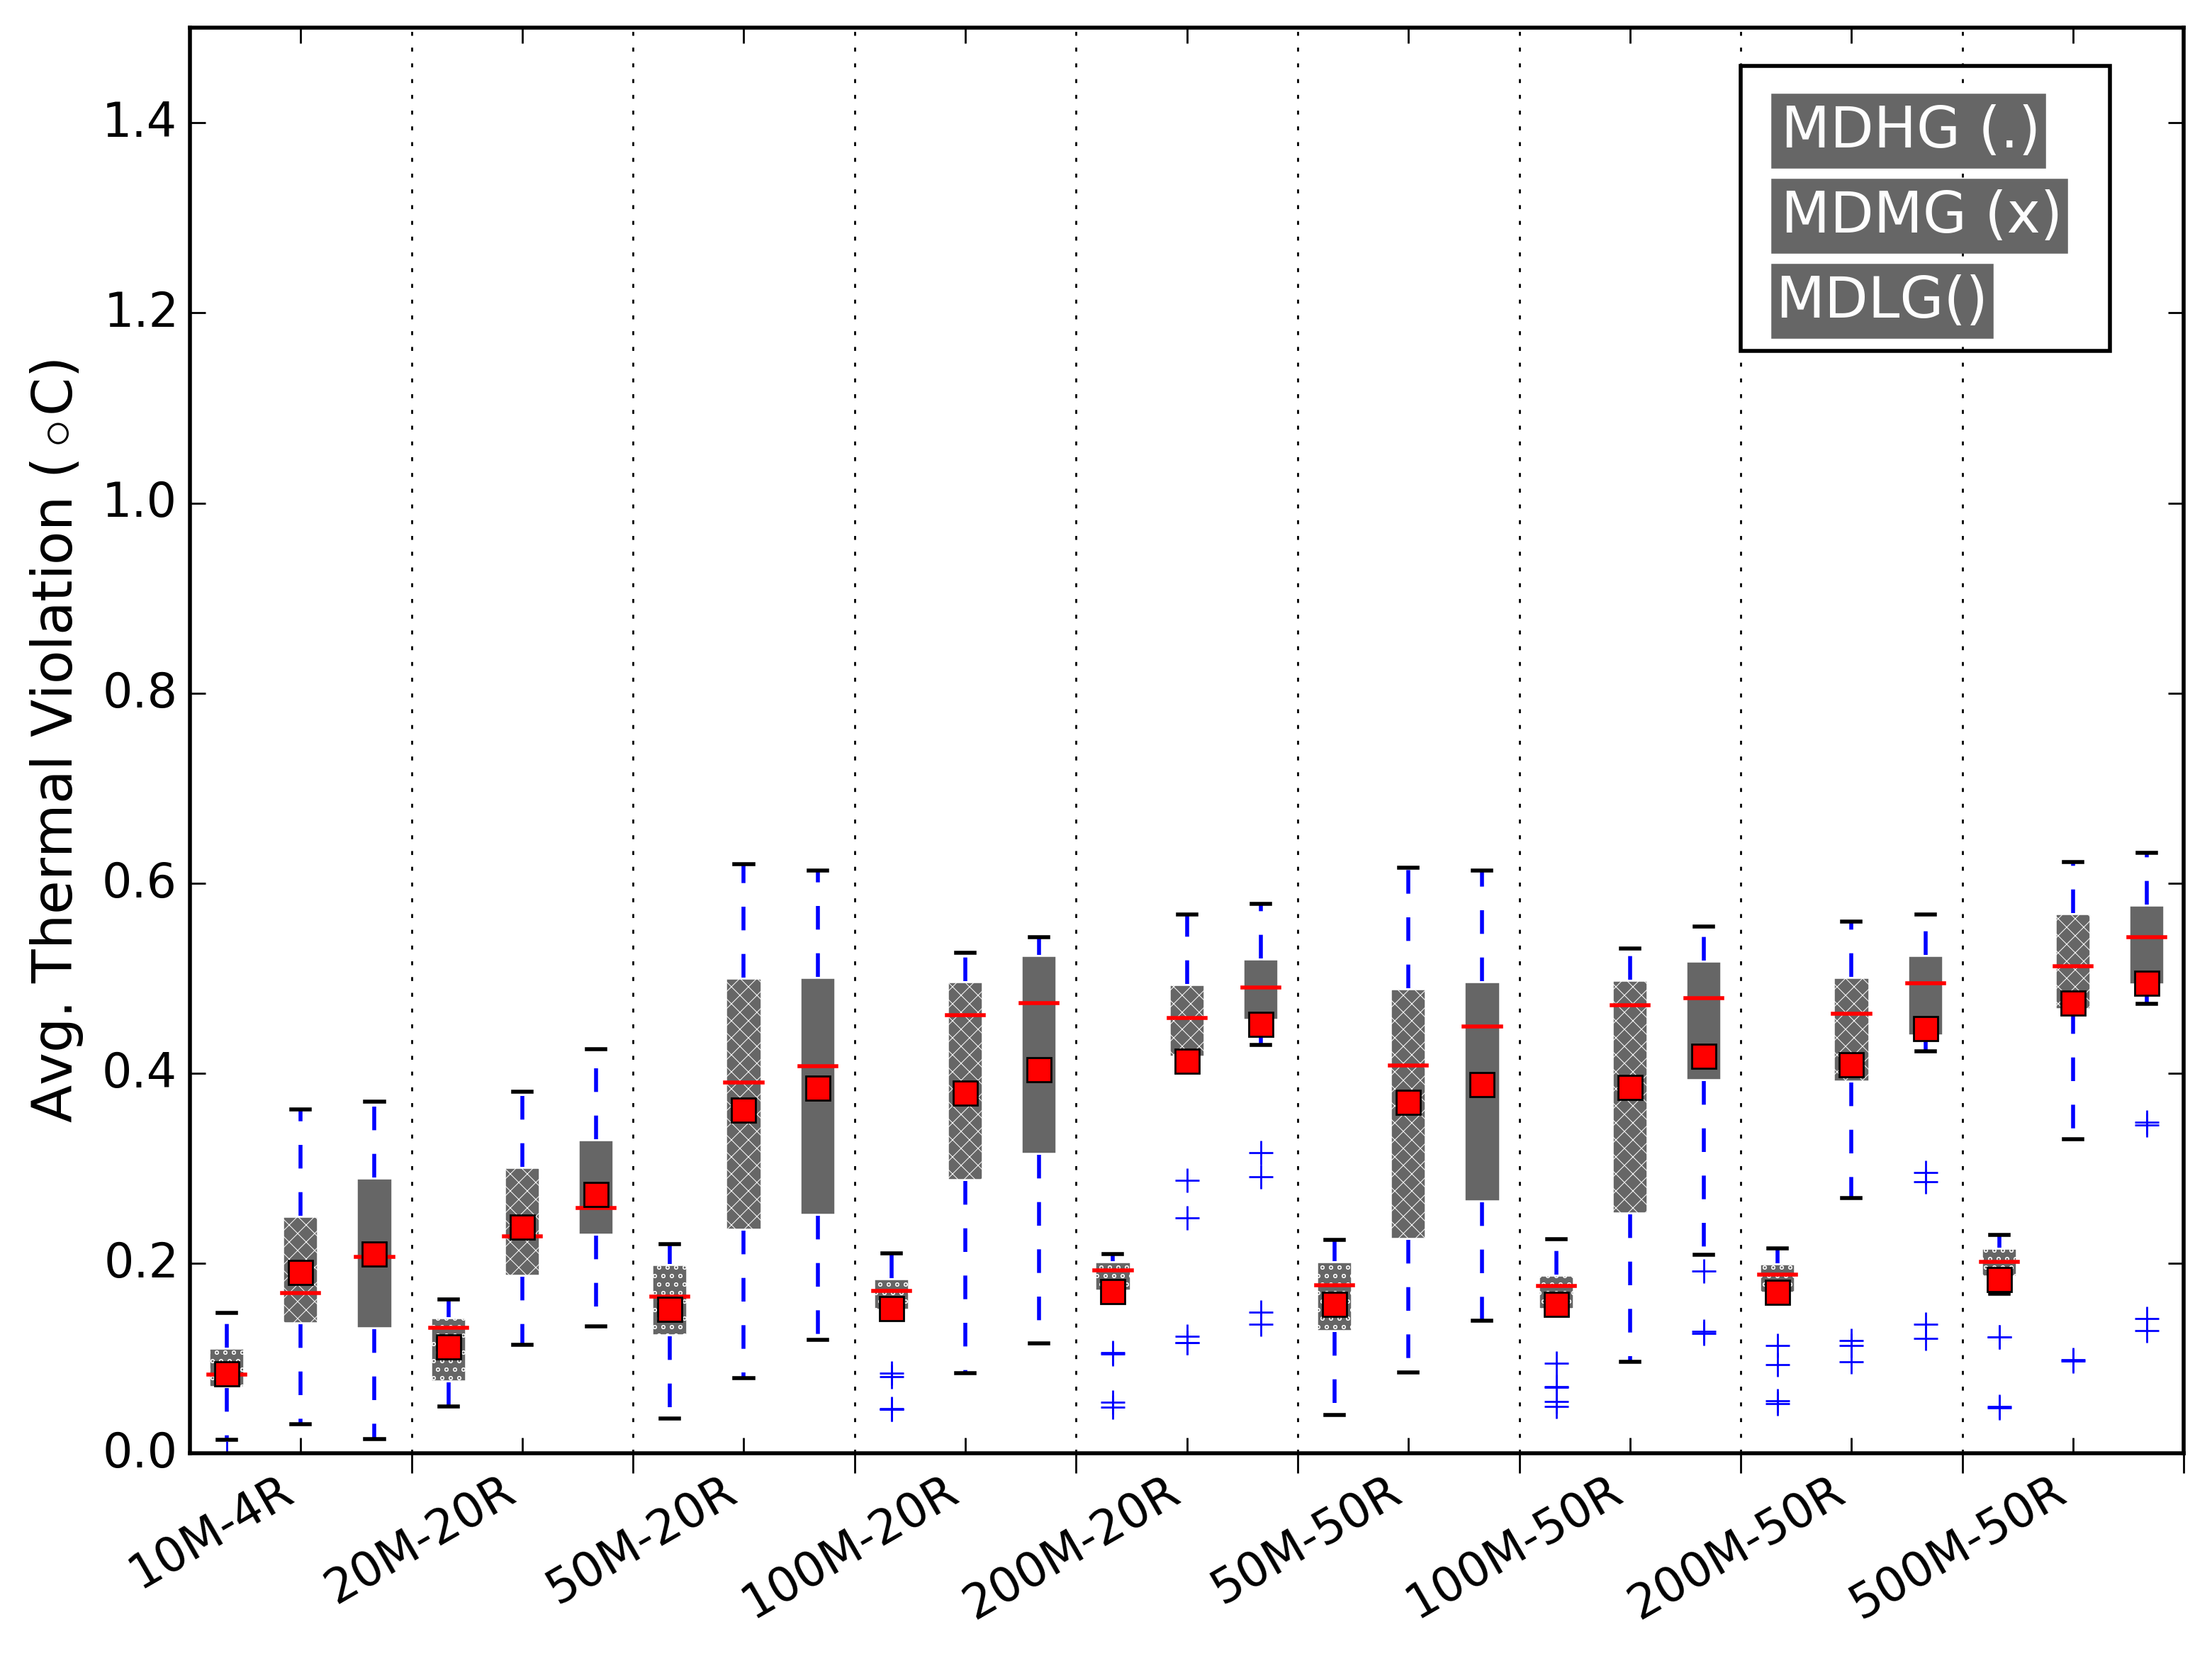
\includegraphics[width=0.6\linewidth]{figs/avg_thermal_violation_diff_temp_flex_def_vs_oarb_medium_boxplot_mtd.png} \\
%(b) Average \\[6pt]
	%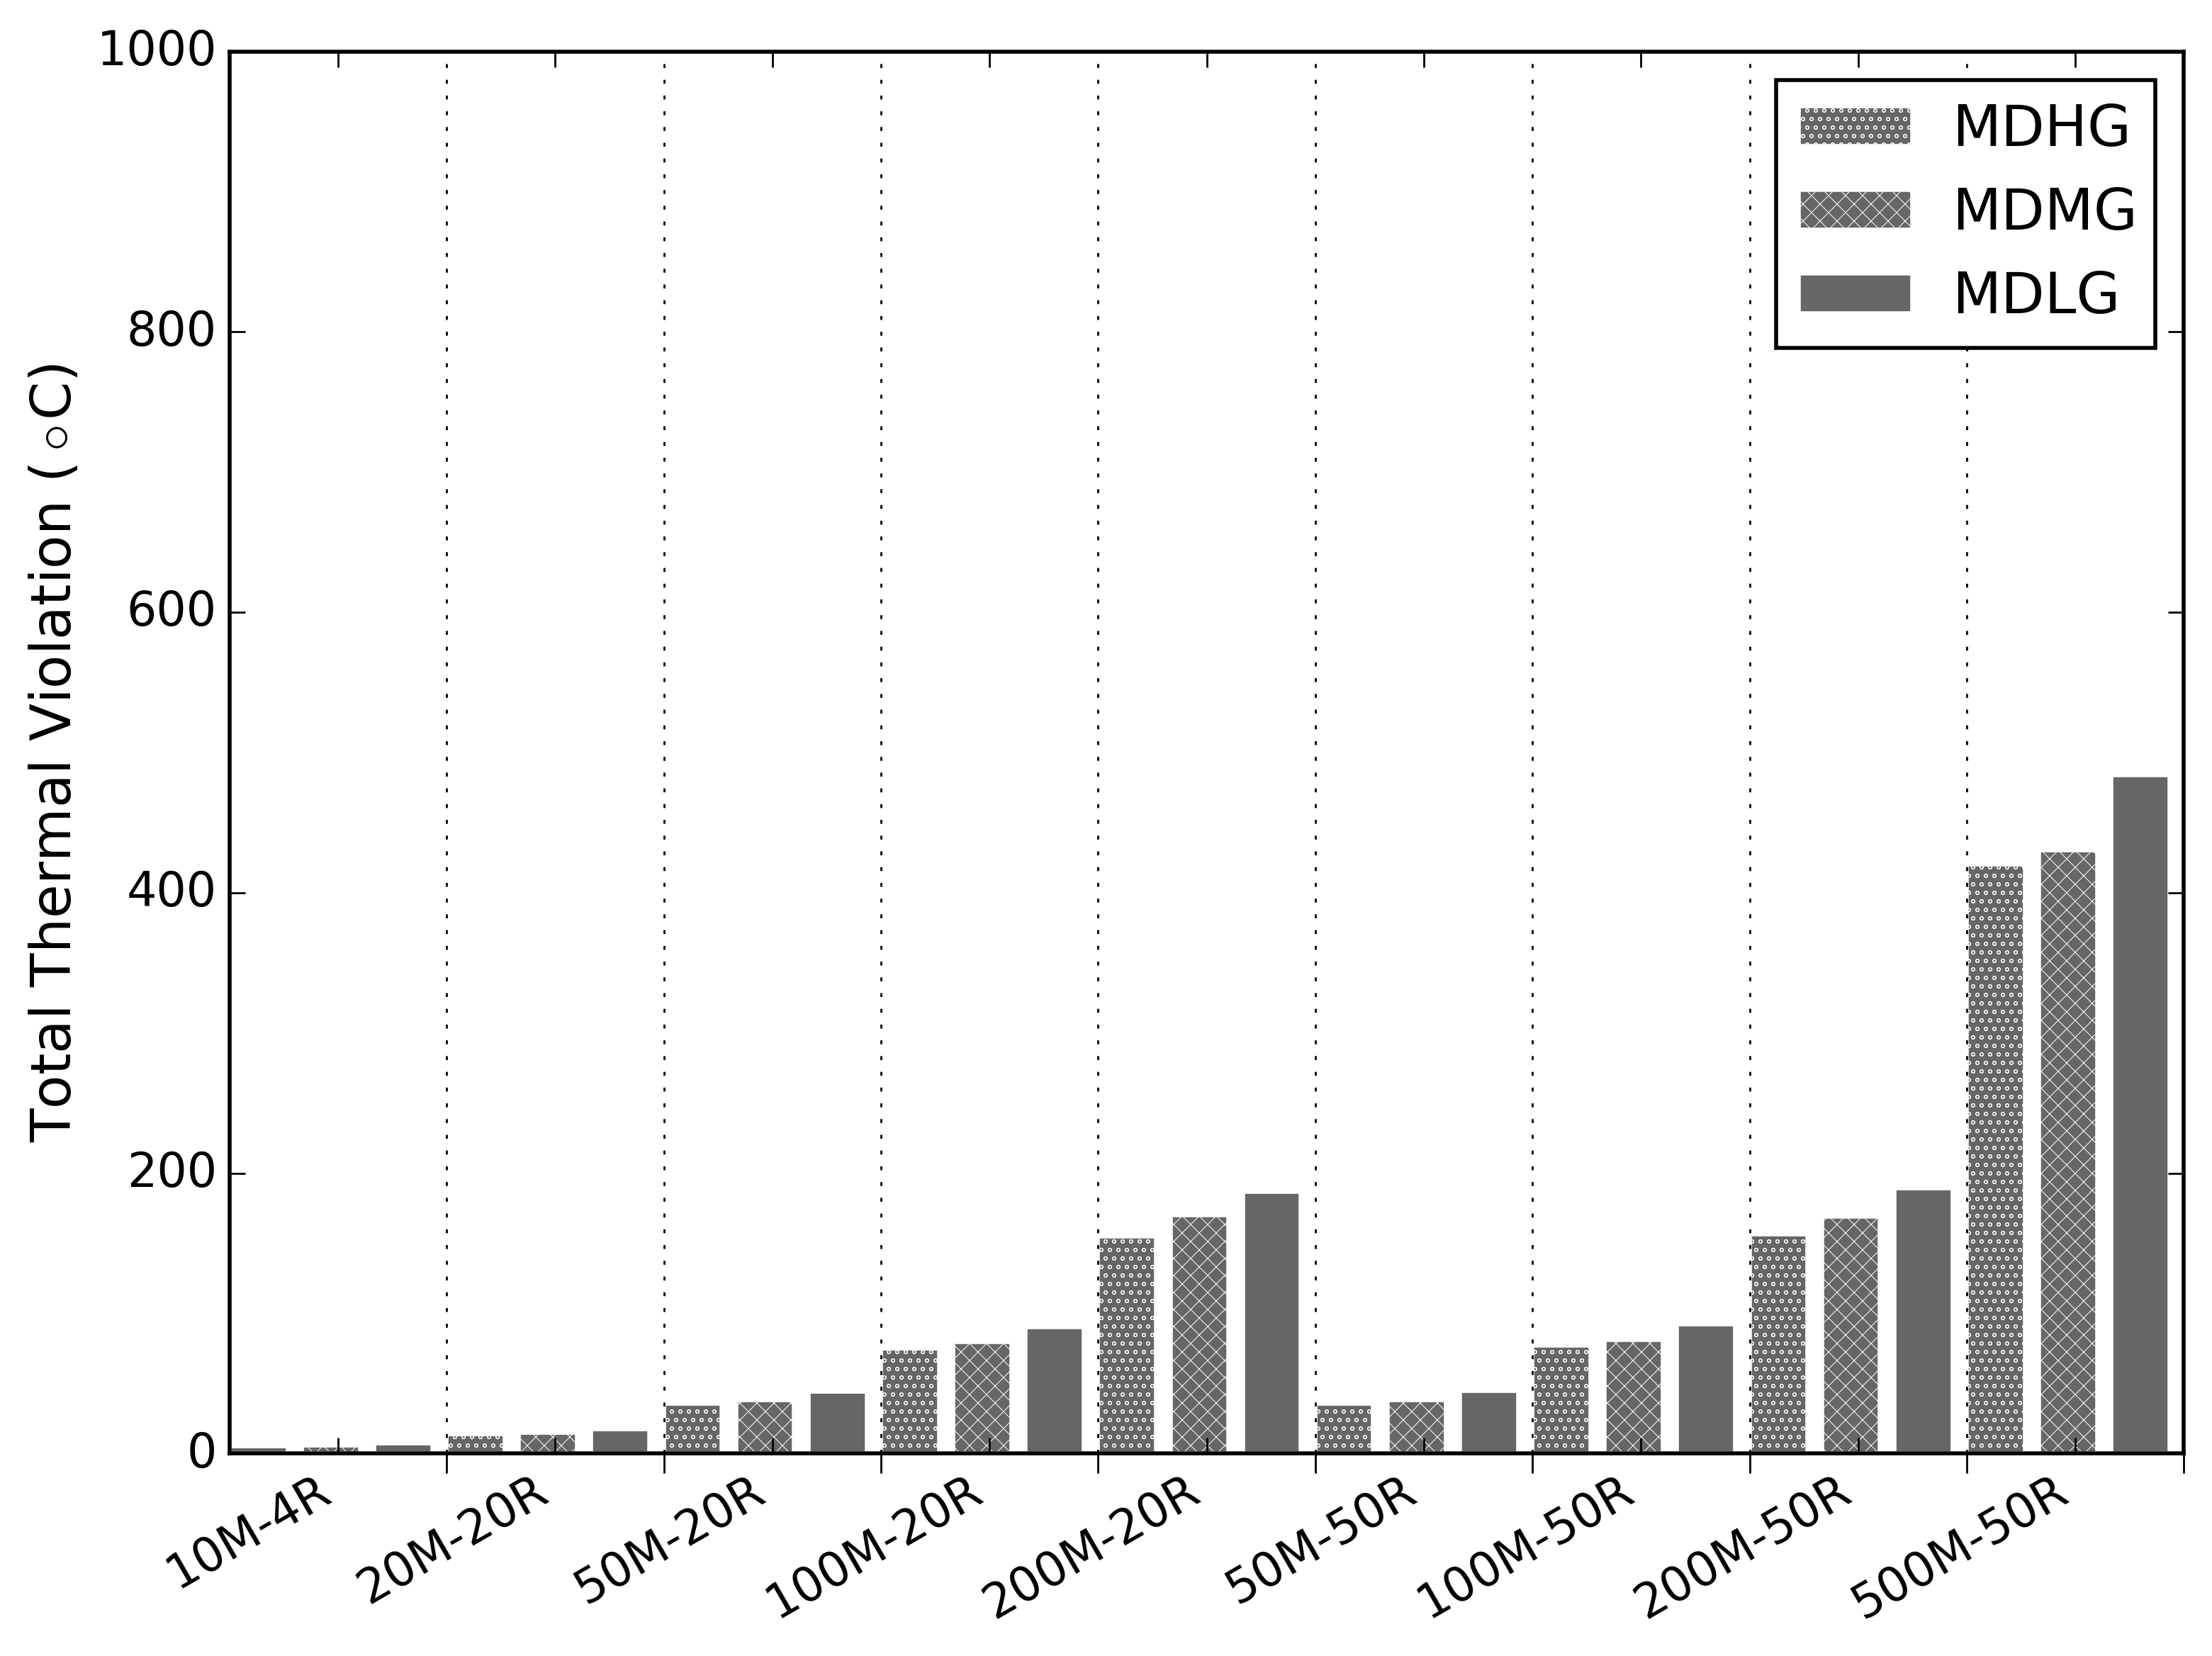
\includegraphics[width=0.6\linewidth]{figs/total_thermal_violation_diff_temp_flex_def_vs_oarb_medium_mtd.png} \\
%(c) Total 
%\end{tabular}
%\caption{MTDA approach - Temperature Deviation vs Robustness to Thermal Comfort (Medium Deviation)}
%\label{fig:atc_mtmr}
%\end{figure}

One important question regarding adaptive temperature control is that of how much thermal comfort is being sacrificed in order to achieve energy savings. While we strive to minimise energy consumption, our model ensures that the occupied temperature bounds are within acceptable range. 
Figure \ref{fig:atc_mt} shows the effects of thermal comfort with the MTDA approach and Figure \ref{fig:atc_ot} depicts the effects with OATA approach. Observe from Figure \ref{fig:atc_mt}(a) that, for the MTDA approach, the maximum temperature deviation is kept below [0.5, 1.5, 2.5]$^\circ$C for [LDLG, MDLG, HDLG] flexibility settings. This is aligned with the occupant's input where the highest temperature violation allowed during the activity is explicitly defined. 

For the OATA-approach, recall that the maximum temperature deviation is linked to the difference between outdoor temperature and the comfort setpoints at each time step. When the gap exceeds or falls below a reasonable comfort bound, it is kept to a minimum of 0.5$^\circ$C and a maximum of 3$^\circ$C. With that setting, we notice from \ref{fig:atc_ot}(a) that the maximum deviation for this approach is always kept to the highest temperature gap allowed in order to optimise energy savings.

As maximum temperature deviation only reflects the violation at some time slot(s) during the activity, we further investigate on the average thermal violation throughout the entire occupied periods. Figure \ref{fig:atc_mt}(b) and \ref{fig:atc_ot}(b) illustrate the average temperature violation. %The MTDA approach shows an average deviation of [0.20,	0.46,	0.72]$^\circ$C for [low, medium, high] settings, whilst the OATA approach depicts [0.46, 0.51, 0.6]$^\circ$C. %Overall the occupied temperature is kept below 1$^\circ$C deviation. %, with a trend of higher deviation if the time flexibility is lesser and the request-to-start time is shorter. 
%However 
The MTDA approach depicts a relatively small gap. On the contrary, the OATA model shows a larger fluctuation between the minimum and the maximum average thermal violation. Overall, the thermal comfort of occupants are not neglected and are kept within reasonable bounds during the entire activity periods. 

We also observe that different level of thermal comfort guarantees lead to varying average temperature violation. In \ref{fig:atc_ot}(b),  the OATA-based HG approach achieves a lower average temperature violation compared to its LG approach. Similar trends are seen from Figure \ref{fig:atc_mtrb} where the MTDA-based MDHG and HDHG approaches also achieve a lower average temperature violation than its respective MDLG and HDLG approaches. Also note that the average thermal violation for the MD approach in Figure \ref{fig:atc_mtrb}(a) is lower than its counterpart in the HD approach in Figure \ref{fig:atc_mtrb}(b). 

Figure \ref{fig:atc_mt}(c) and \ref{fig:atc_ot}(c) show the total thermal violation for activities in each group. Observe that the gap between low and high flexibility for the MTDA-approach is larger than that of the OATA-approach. This further affirms that the energy savings is directly proportional to the cumulative temperature deviation allowed, and that both graphs show similar pattern with that of in Figure \ref{fig:atc_eg}.


\subsection{Model Feasibility} \label{sec:feasibility}

Finally, we study the feasibility of online scheduling with fixed and adaptive temperature control, respectively. As highlighted in Chapter \ref{cha:online}, many instances are infeasible when the request-to-start time less than 1 hour with fixed temperature control (see Figure \ref{fig:def_feas}). In this section, we investigate the impact of adaptive temperature control on solution feasibility in our online approach.

Figure~\ref{fig:mtd_deviate}-\ref{fig:mtd_mfhr} show the percentage of feasible solutions generated by different MTDA and OATA configurations. 
Altogether, the MTDA-approach in Figure ~\ref{fig:mtd_deviate} solves 76\% of the instances whilst the OATA-approach in Figure \ref{fig:atc_of} solves 68\% of the instances that are deemed unsolvable under the fixed temperature control regime. 

Figure \ref{fig:mtd_mfmr} and \ref{fig:mtd_mfhr} show an obvious trend that more feasible solutions are generated when the comfort guarantee reduces, and vice versa. In contrast to the fixed setpoints approach, the model with adaptive temperature control is able to solve many of these problem instances, and even generates some feasible solutions when the requests arrive just 10 minutes prior to the earliest activity start time. This is mainly due to the relaxation of the temperature setpoints. Overall, The number of feasible solutions increases proportionally to the temperature flexibility. 


\begin{figure}
\begin{tabular}{ccc}
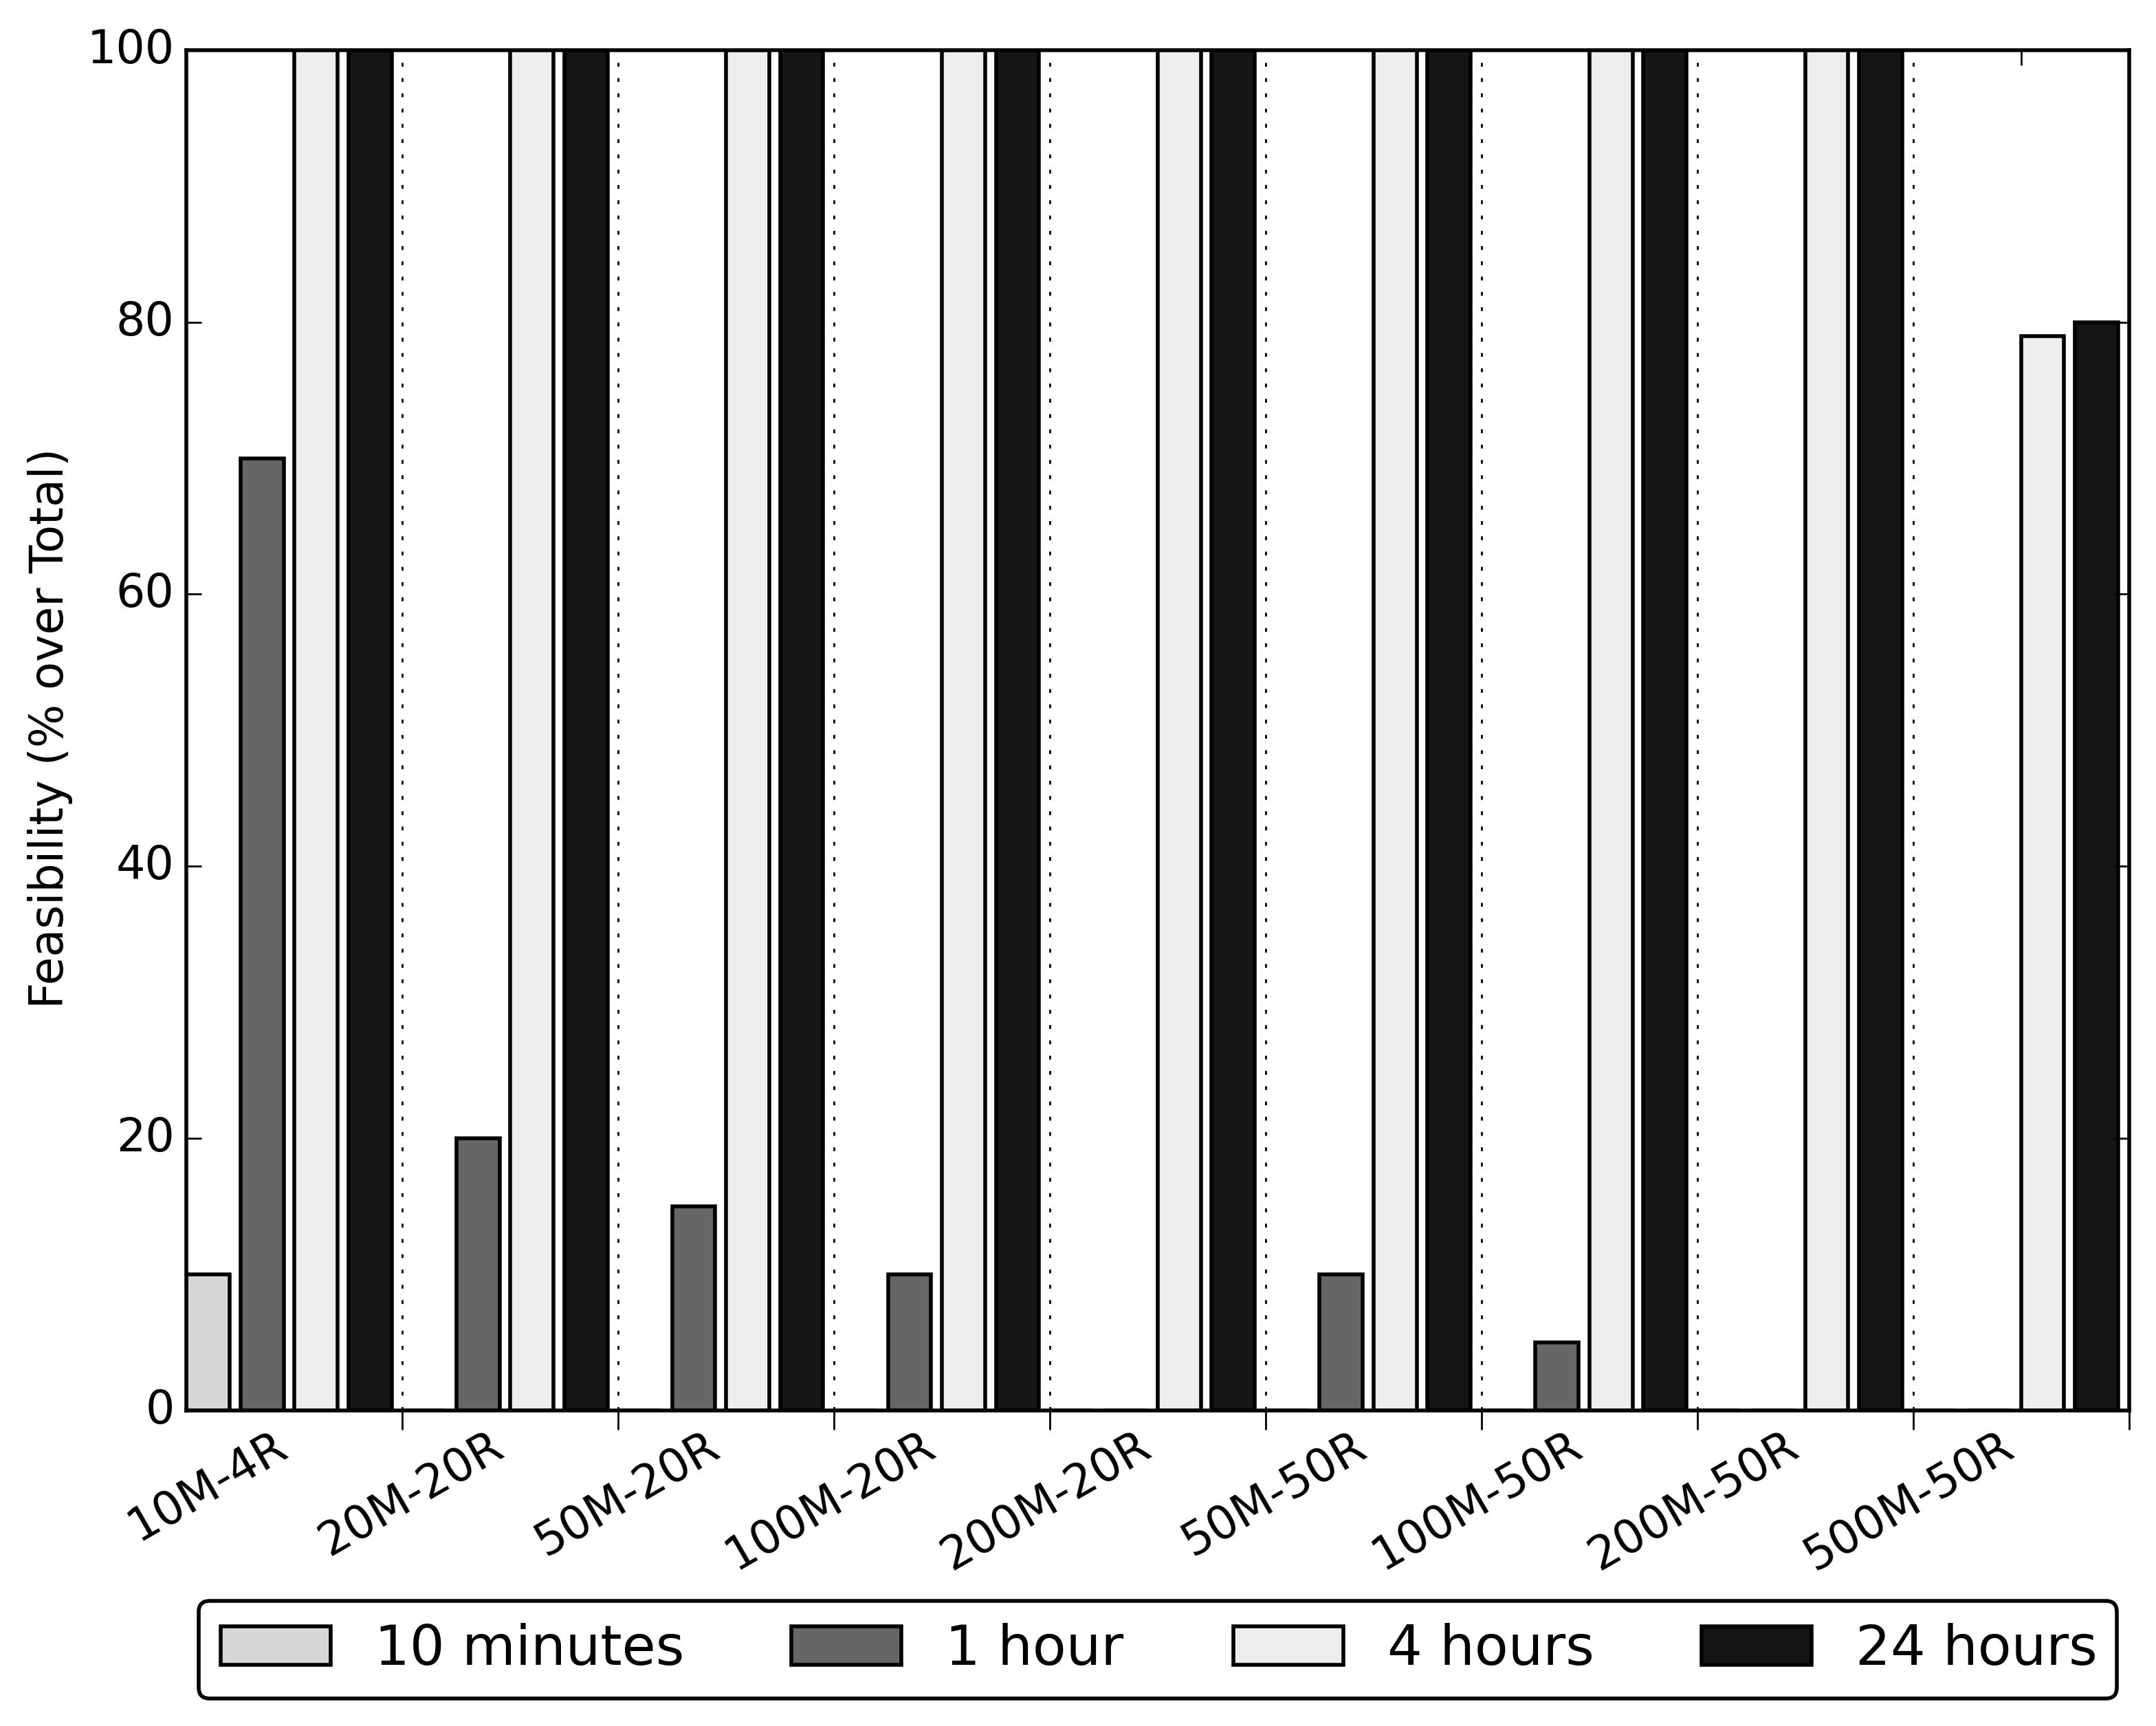
\includegraphics[width=.30\linewidth,keepaspectratio]{figs/feasibility_cvs_oarb_ld_mtd.png} &
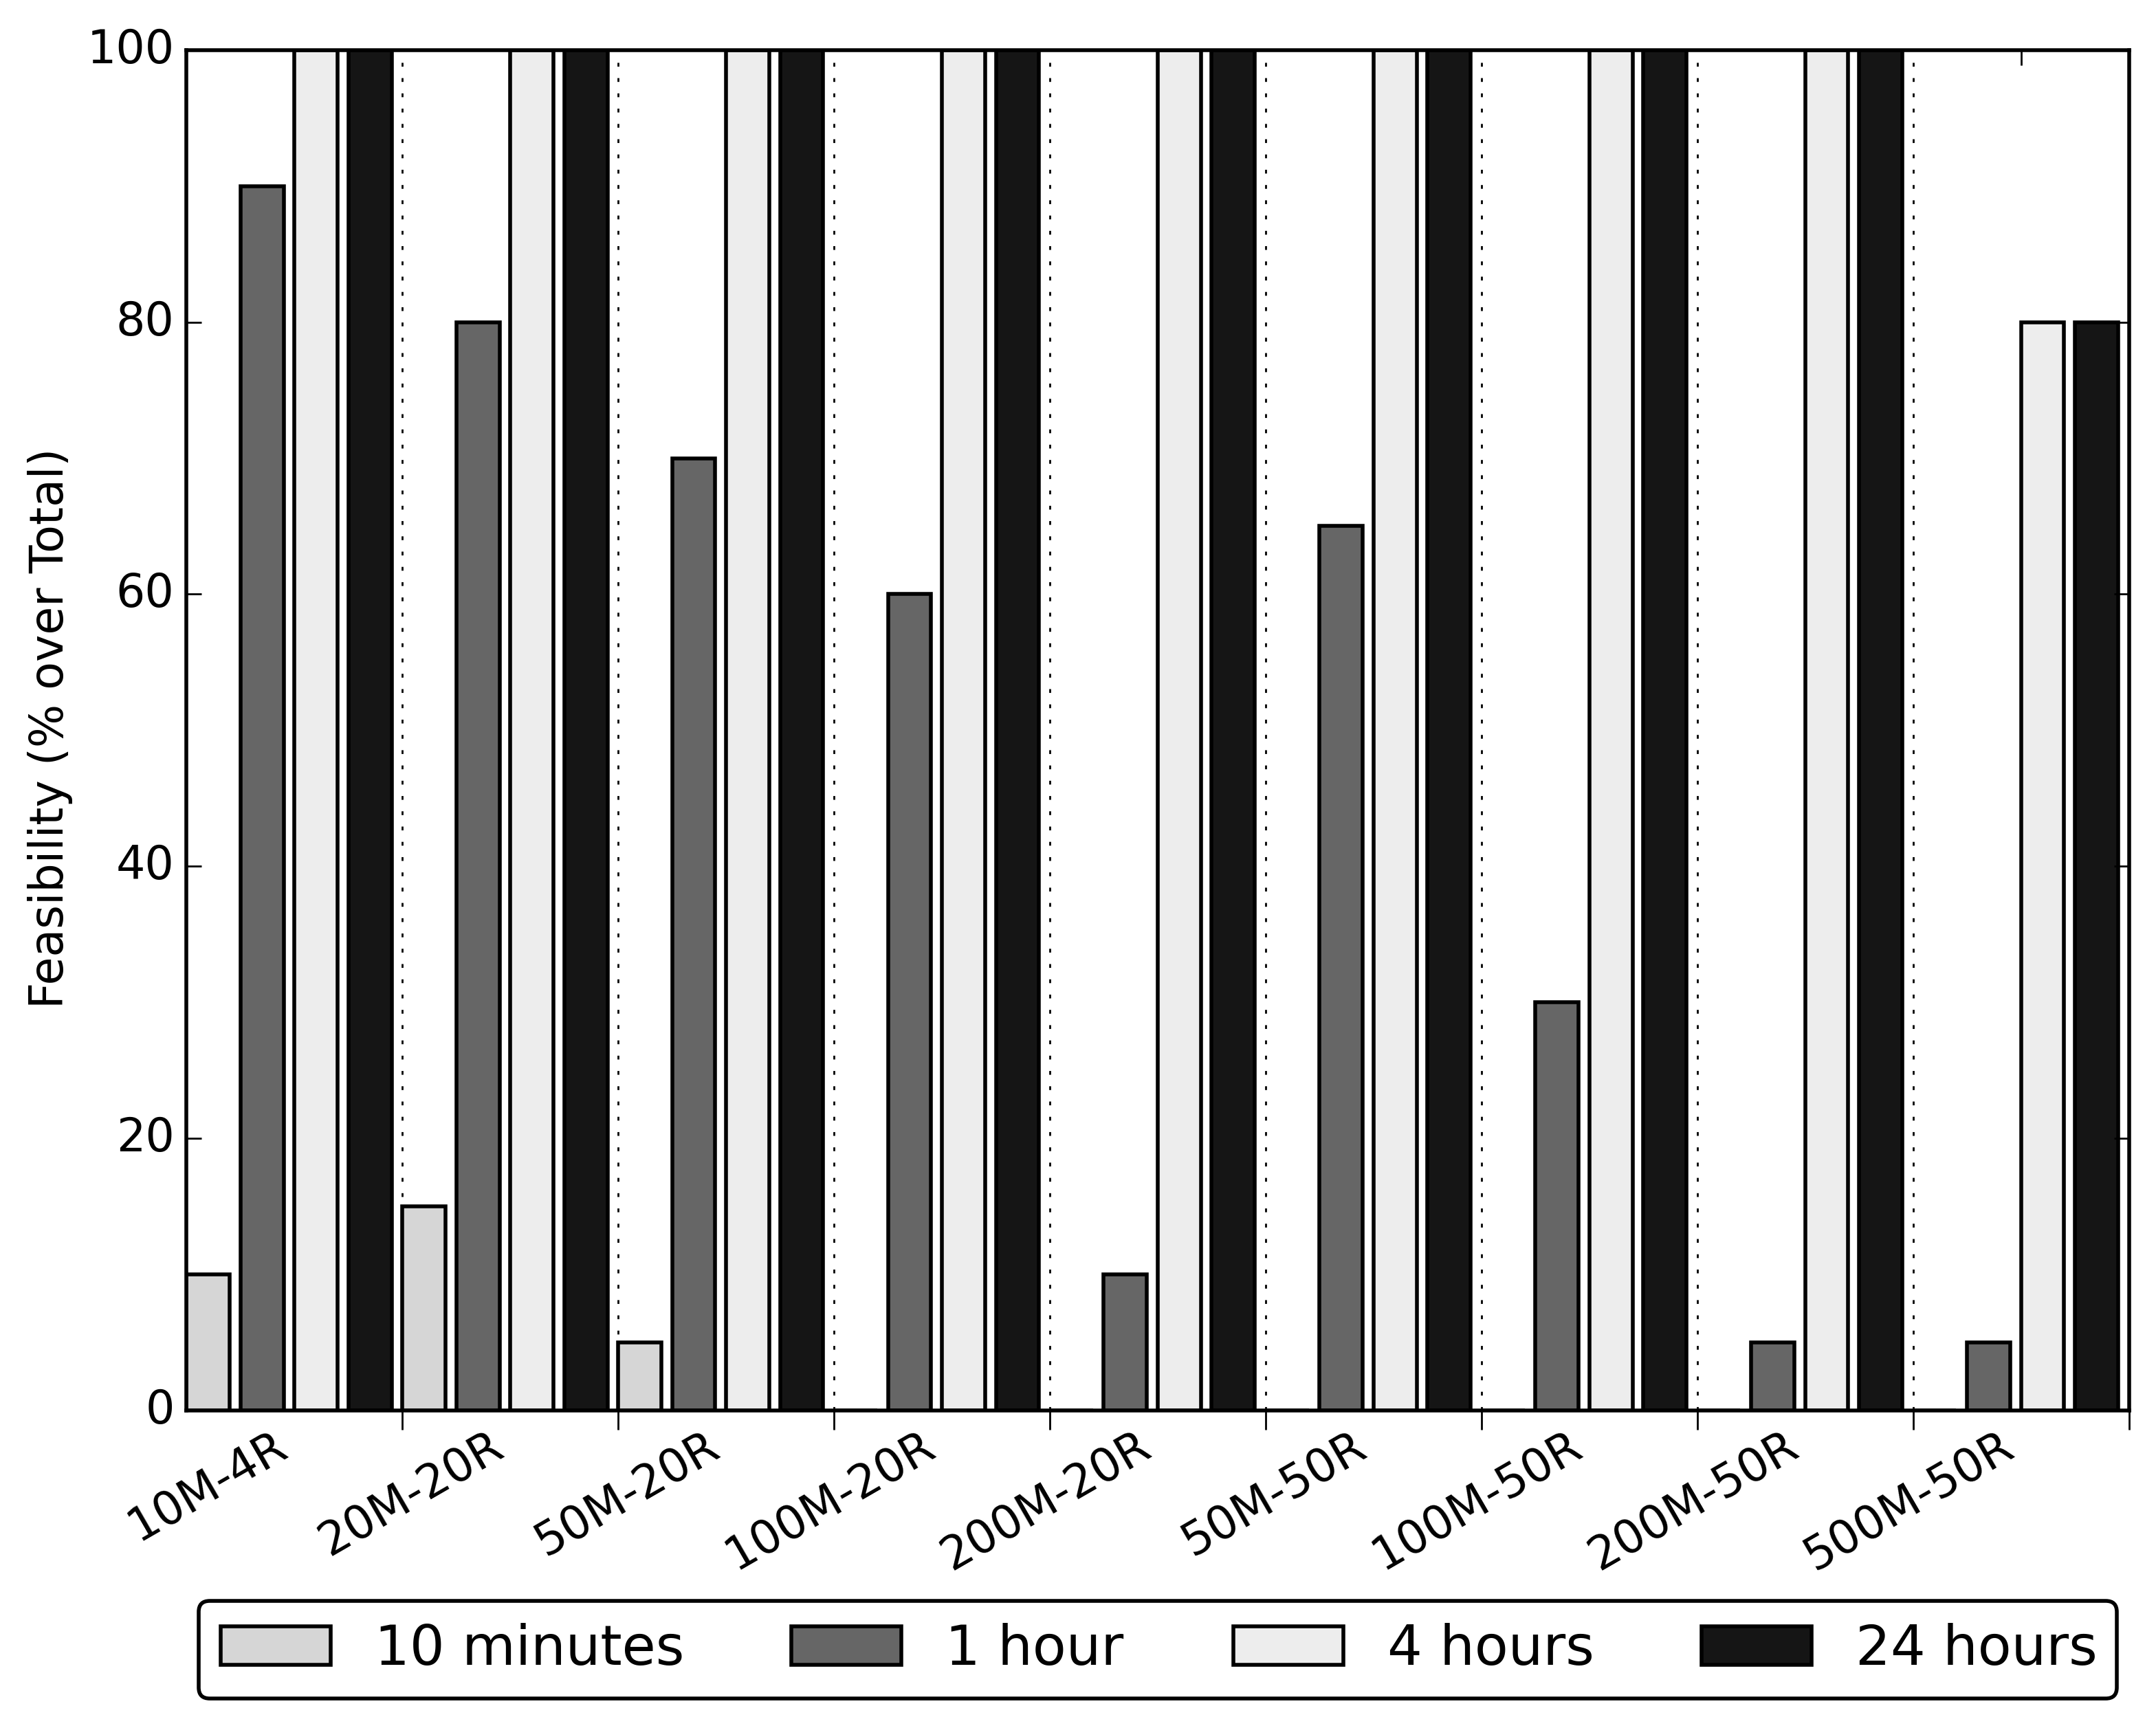
\includegraphics[width=.30\linewidth,keepaspectratio]{figs/feasibility_cvs_oarb_md_mtd.png} &
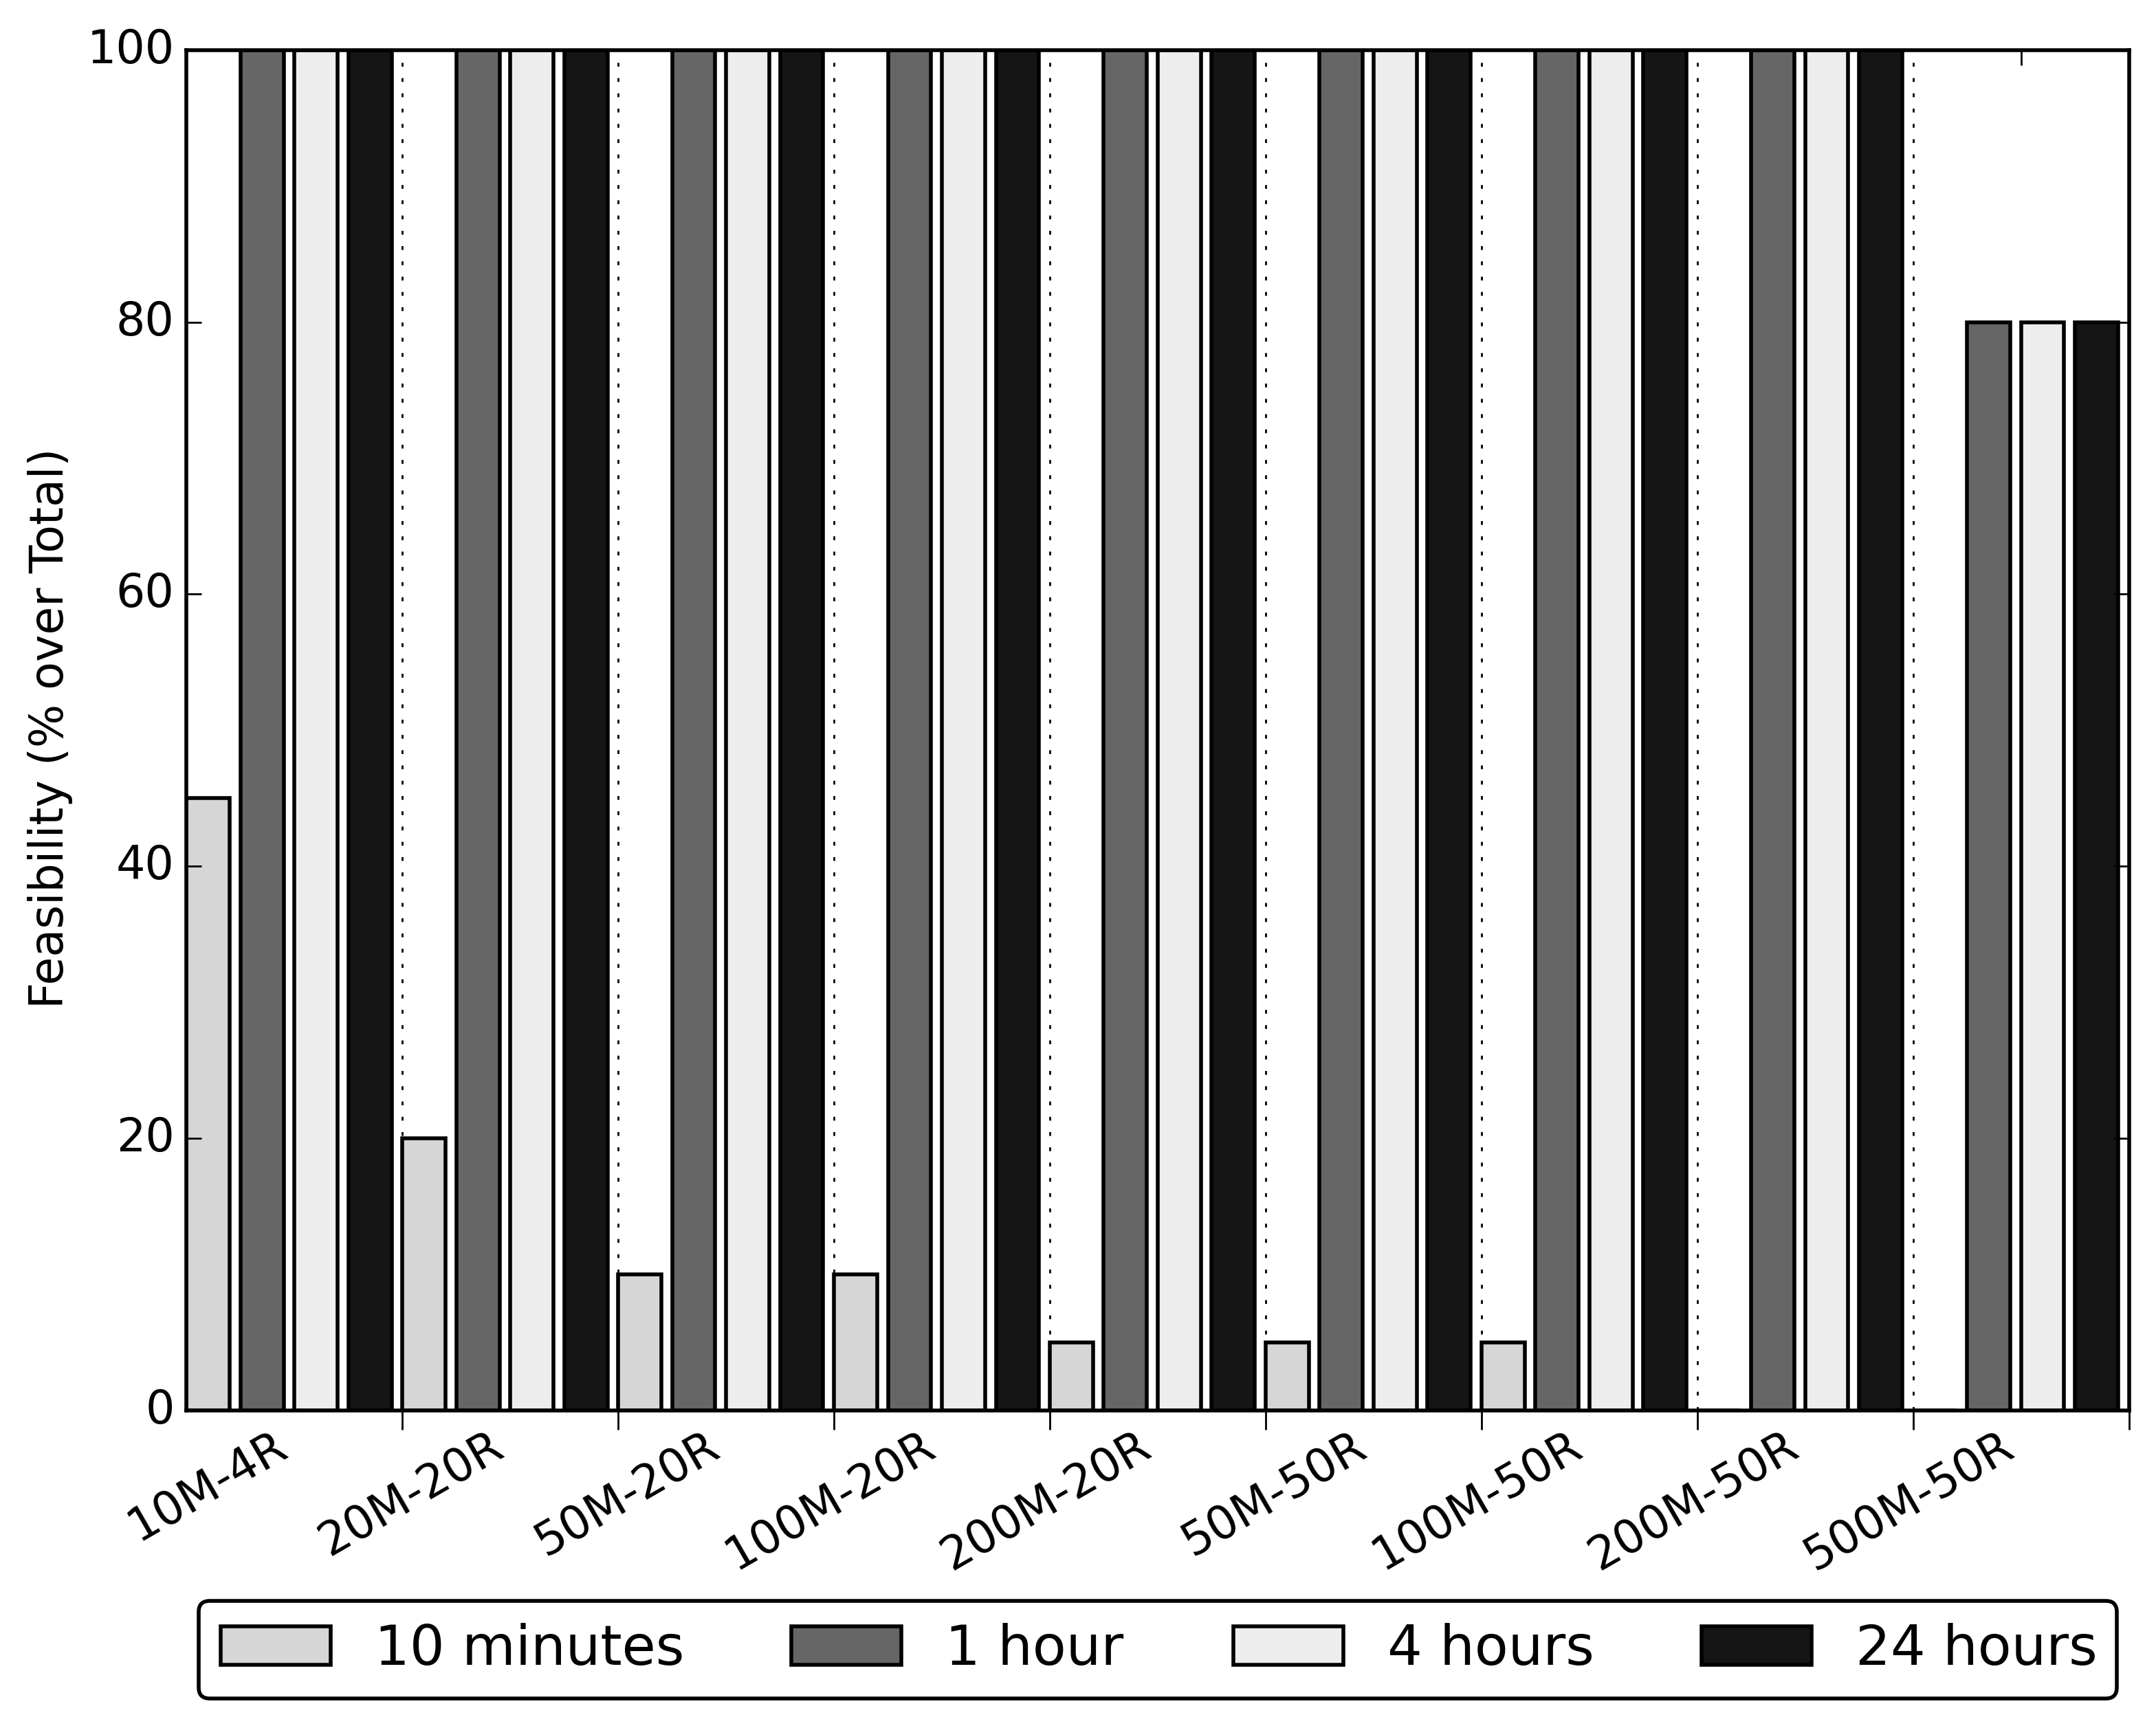
\includegraphics[width=.30\linewidth,keepaspectratio]{figs/feasibility_cvs_oarb_hd_mtd.png} \\
(a) LDLG & (b) MDLG & (c) HDLG
\end{tabular}
\caption{MTDA approach - solution feasibility}
\label{fig:mtd_deviate}
\end{figure}

\begin{figure}
\begin{tabular}{ccc}
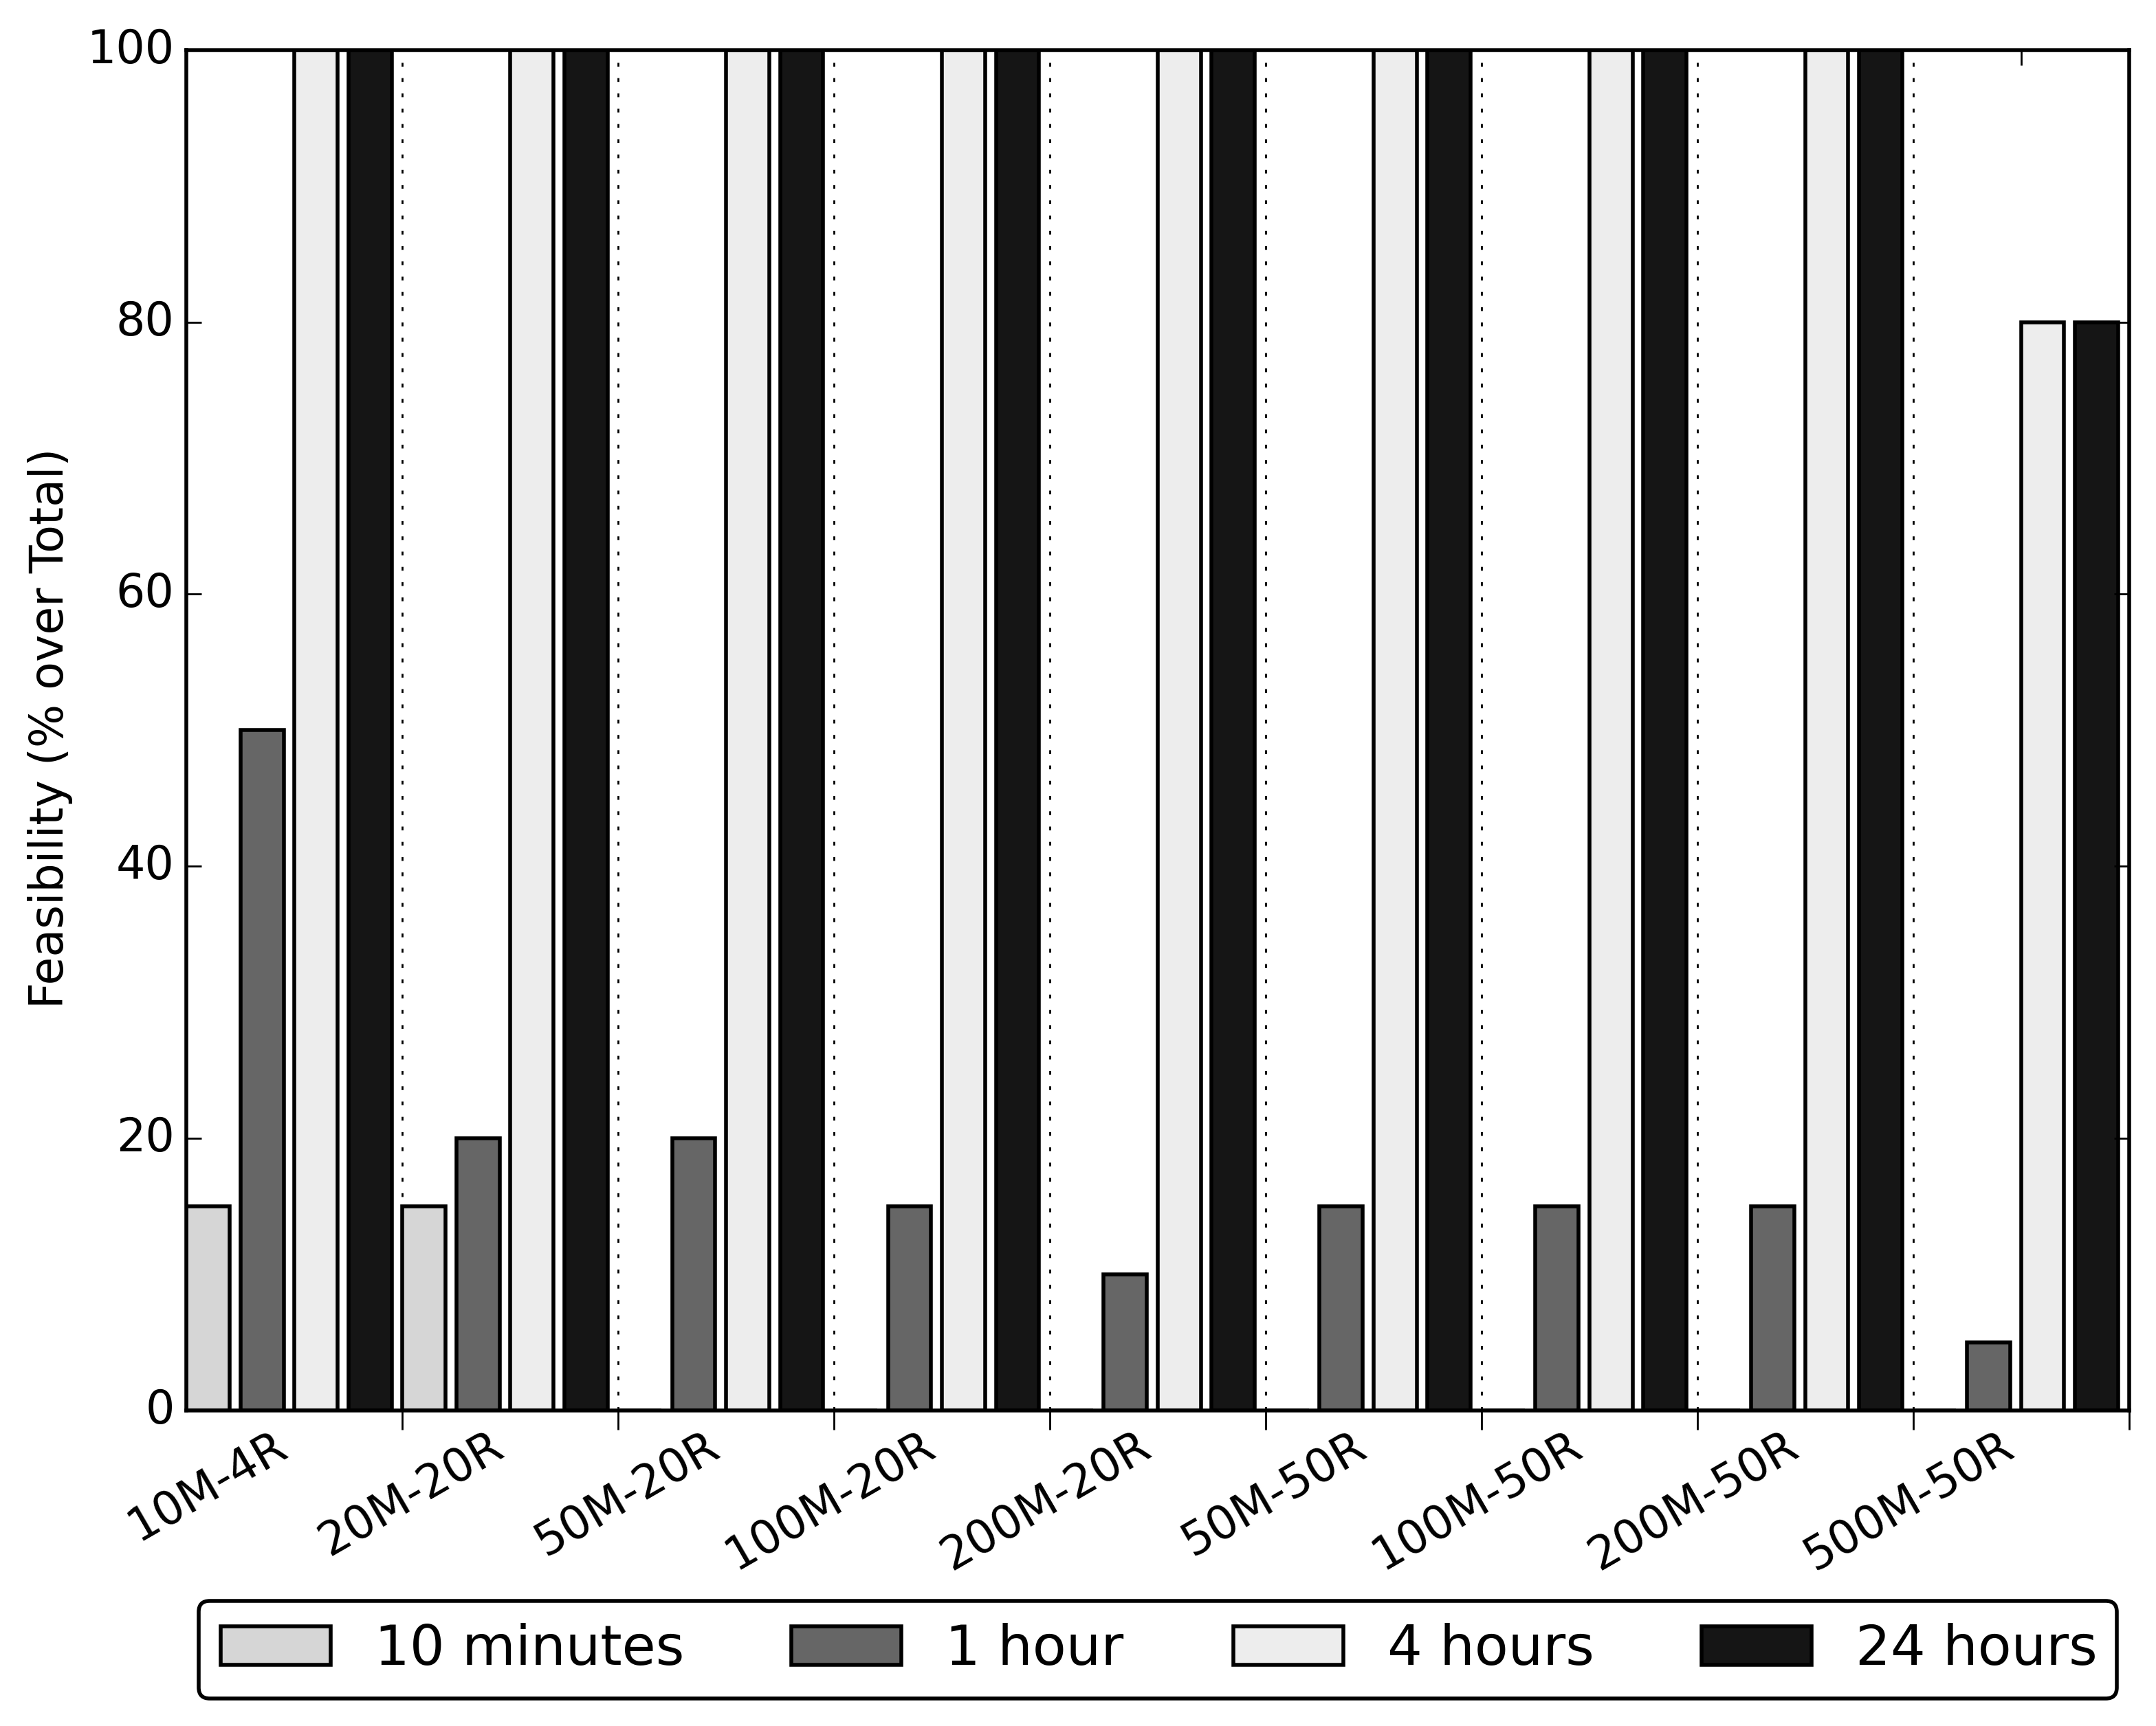
\includegraphics[width=.30\linewidth,keepaspectratio]{figs/feasibility_cvs_oarb_high_oat.png} &
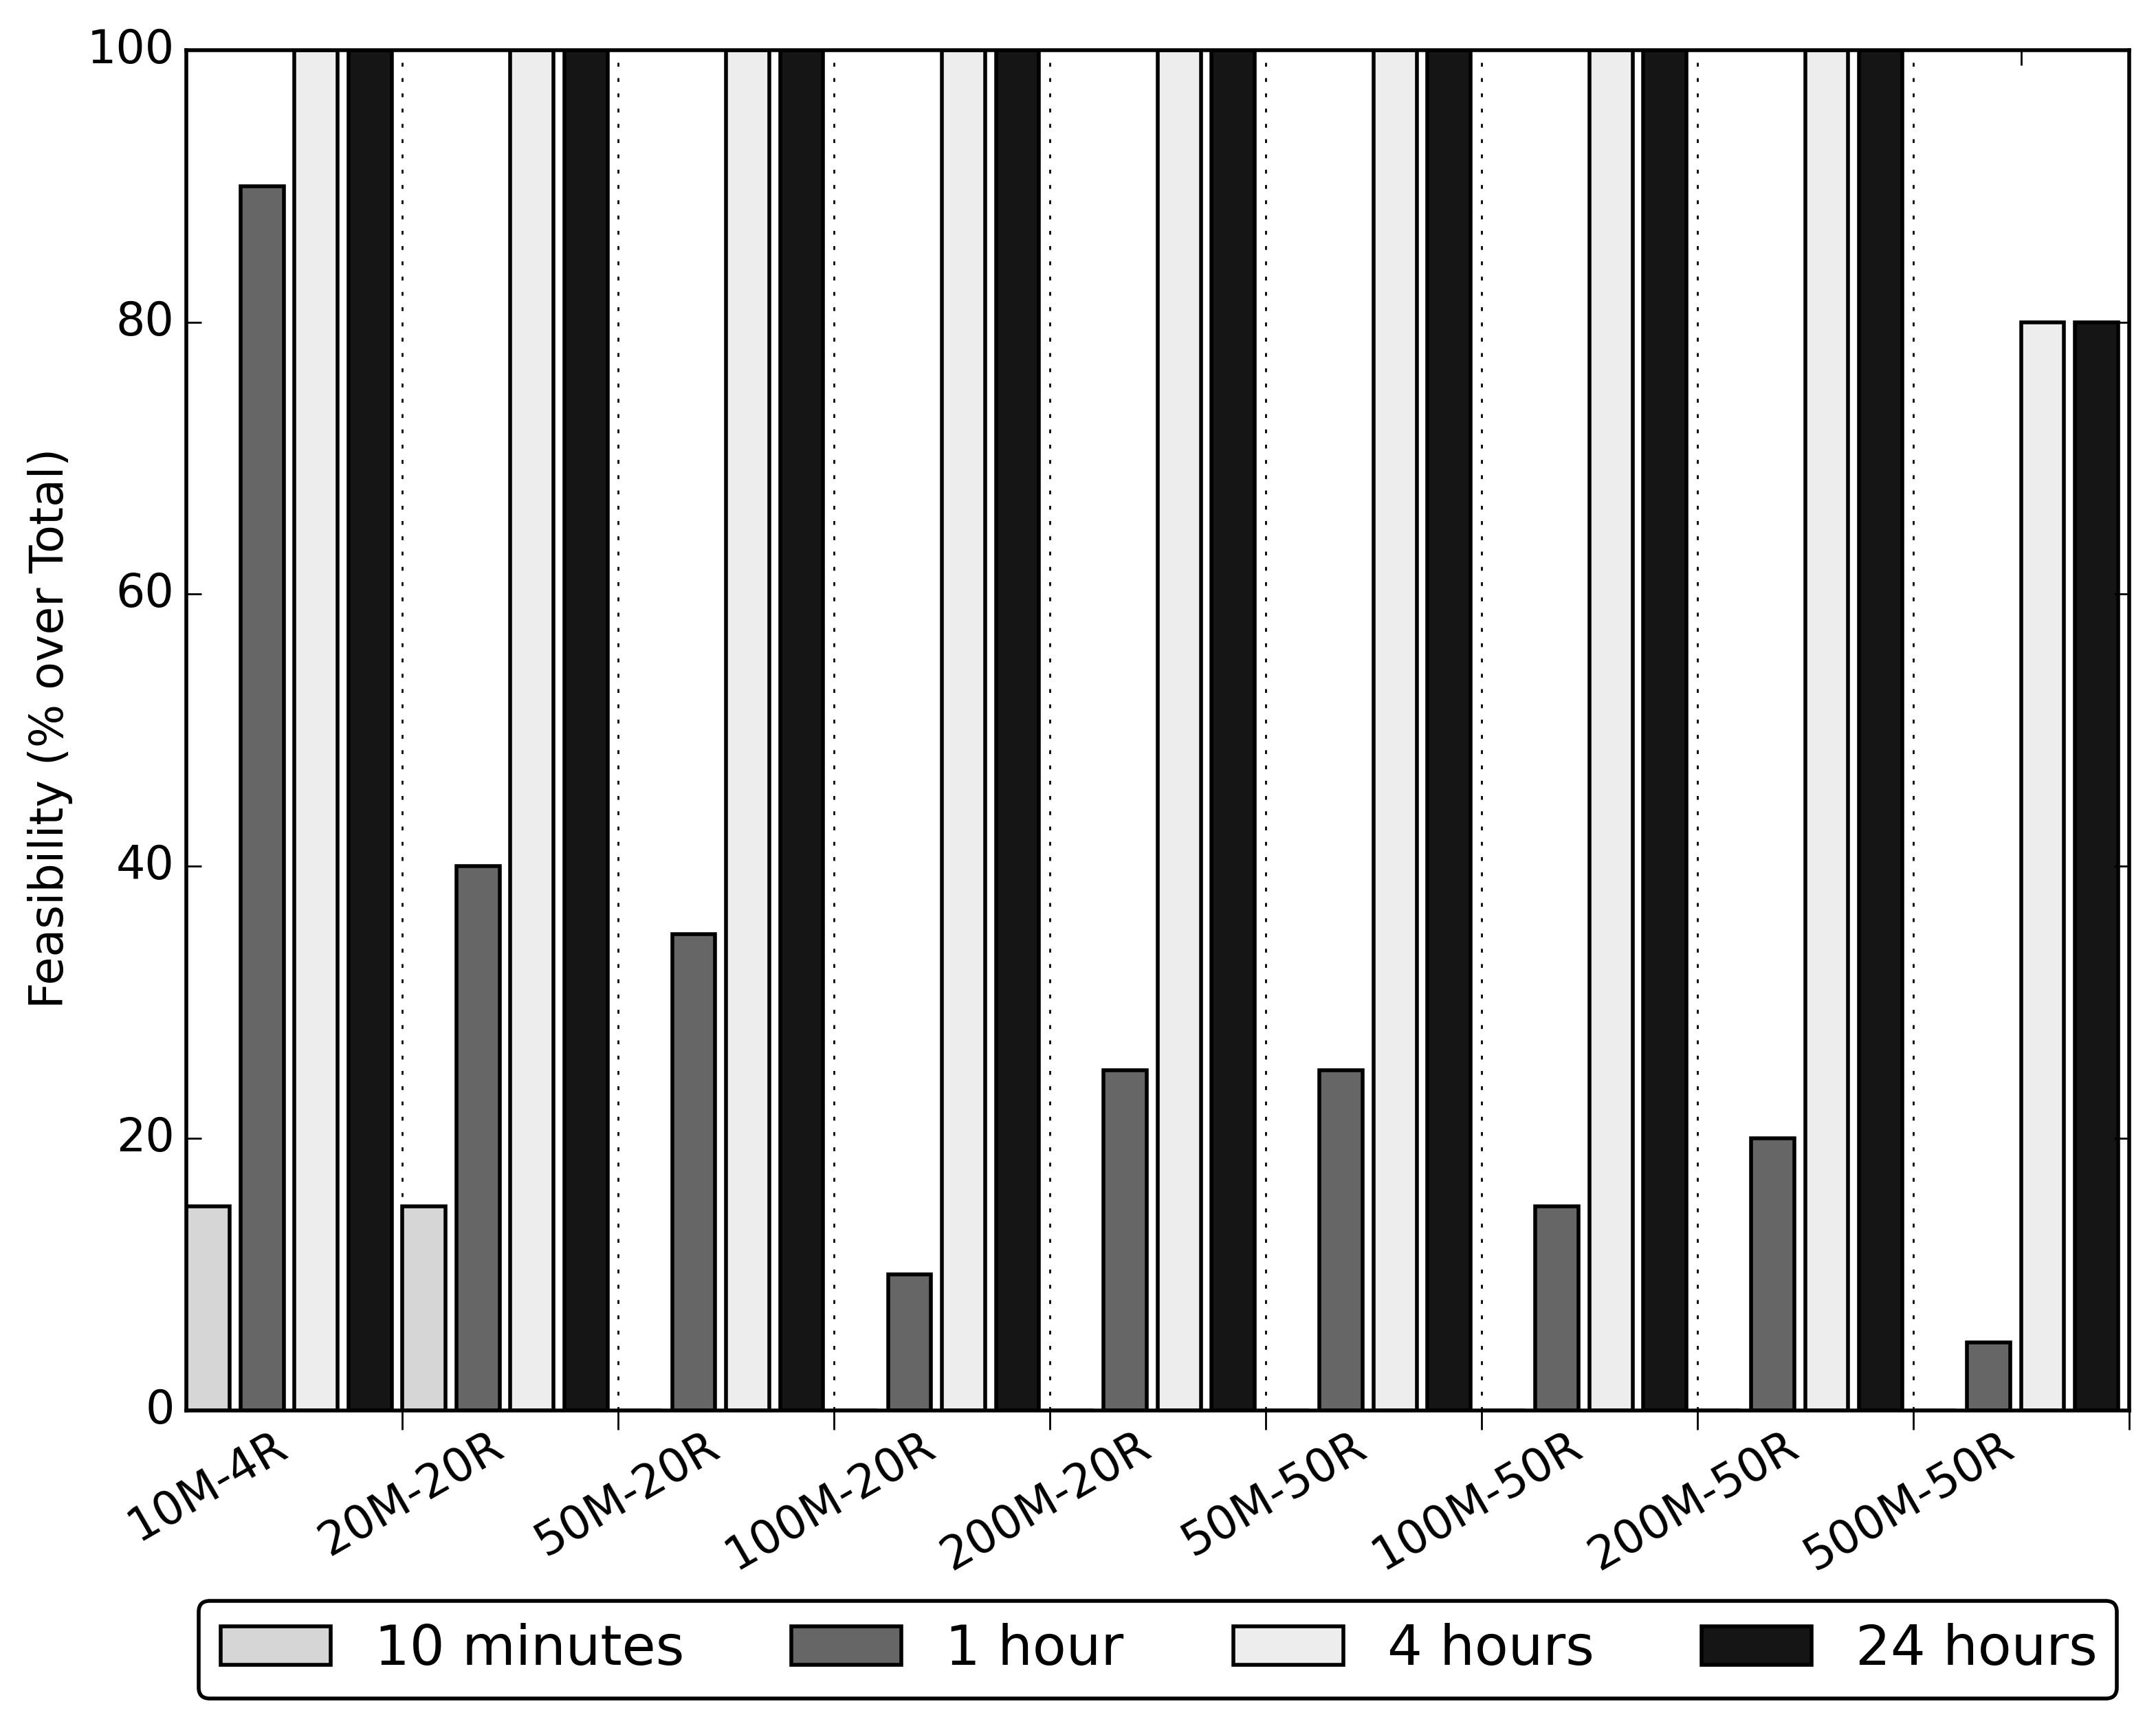
\includegraphics[width=.30\linewidth,keepaspectratio]{figs/feasibility_cvs_oarb_medium_oat.png} &
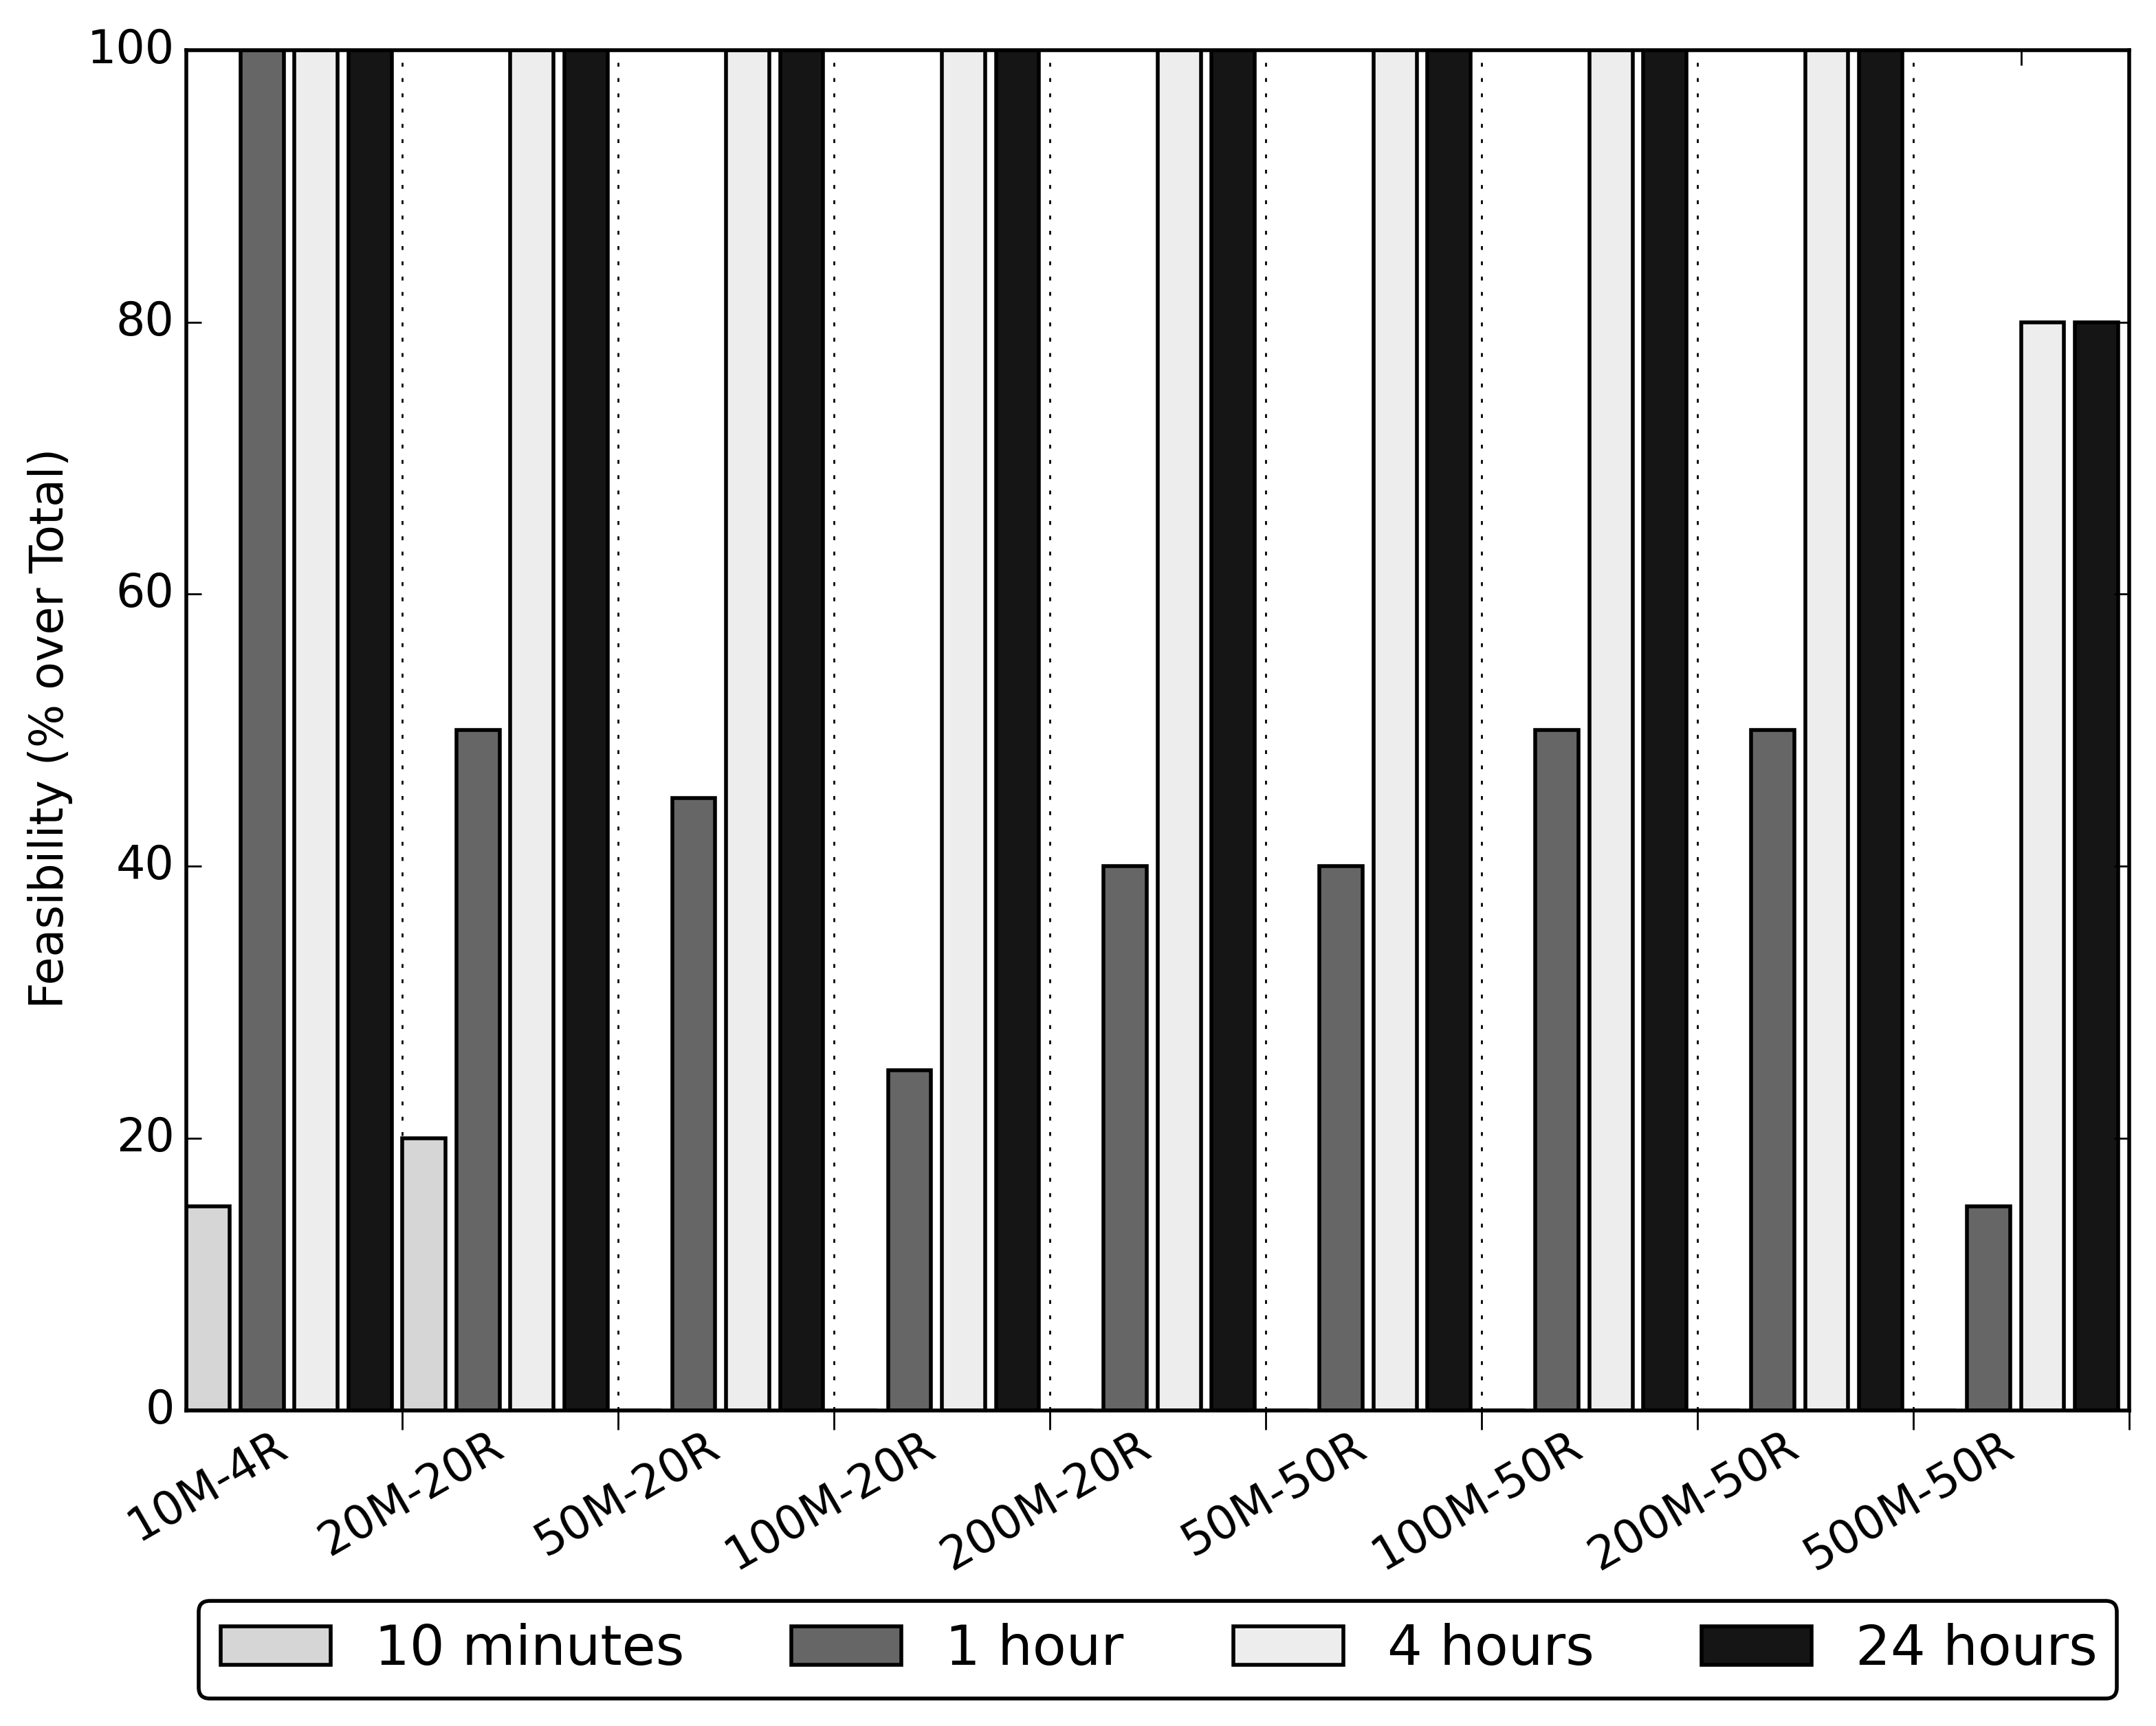
\includegraphics[width=.30\linewidth,keepaspectratio]{figs/feasibility_cvs_oarb_low_oat.png} \\
(a) HG & (b) MG & (c) LG
\end{tabular}
\caption{OATA approach - solution feasibility}
\label{fig:atc_of}
\end{figure}

\begin{figure}
\begin{tabular}{ccc}
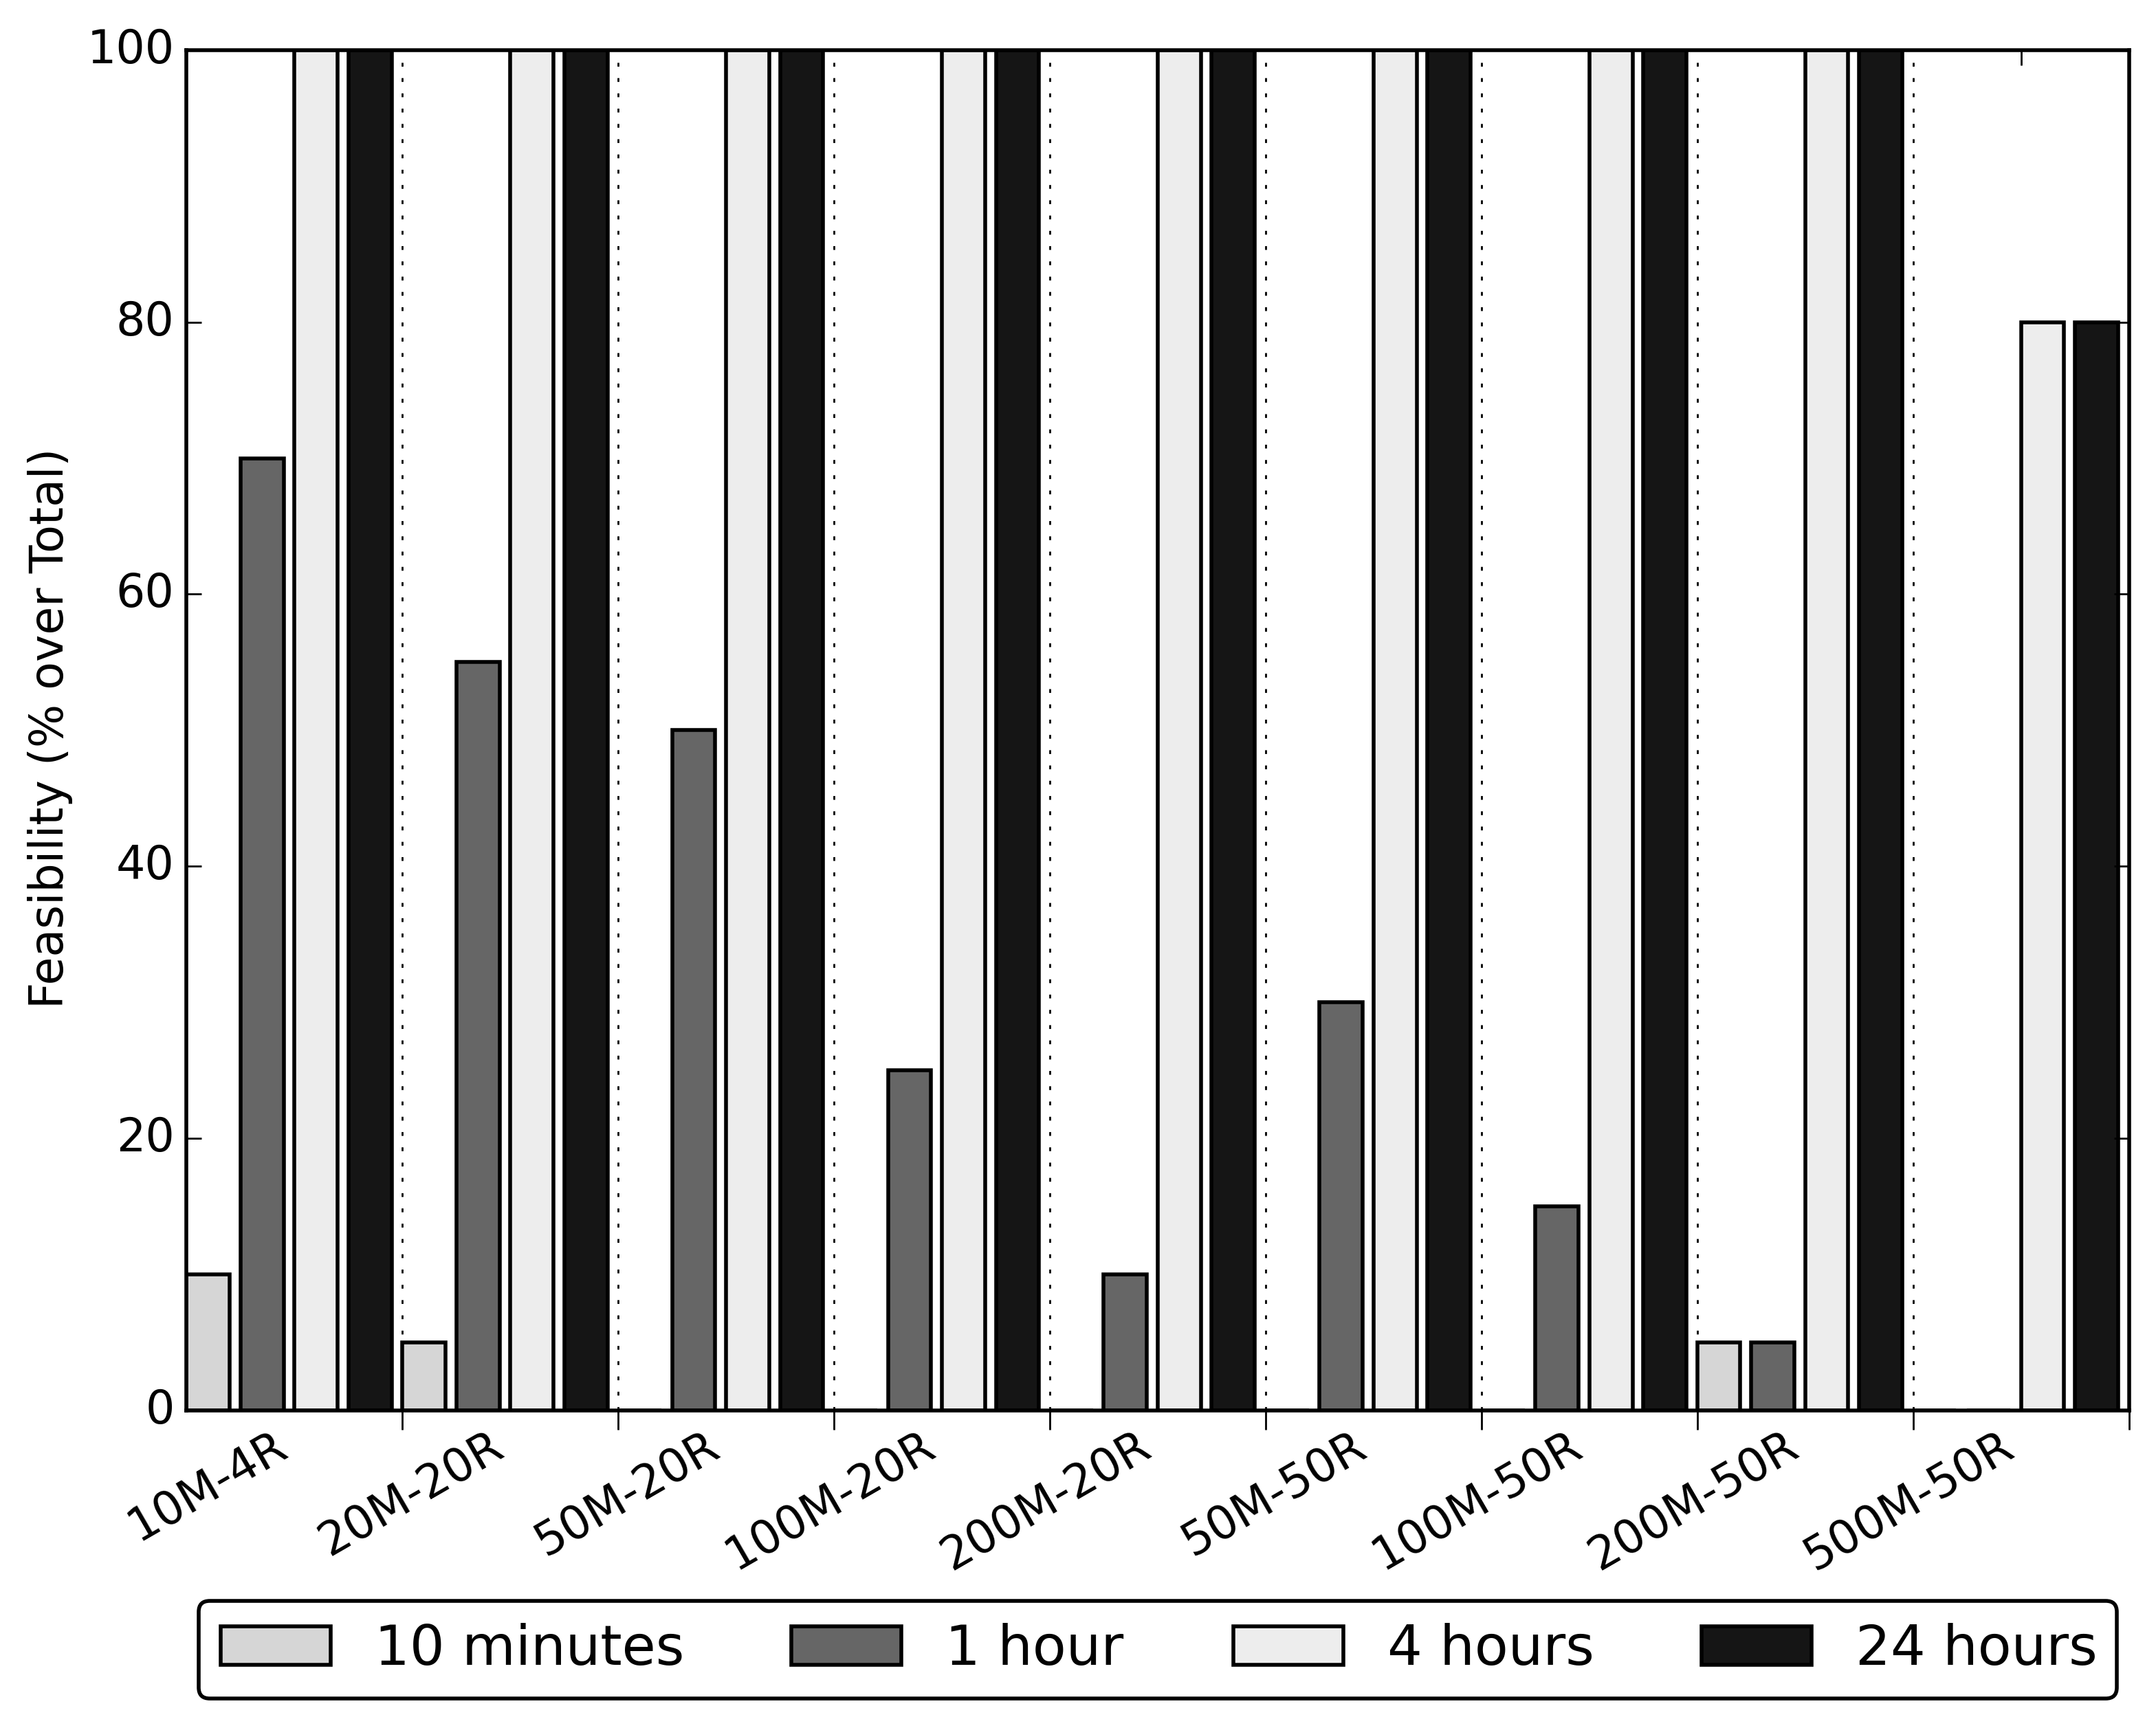
\includegraphics[width=.30\linewidth,keepaspectratio]{figs/feasibility_cvs_oarb_medium_highr_mtd.png} &
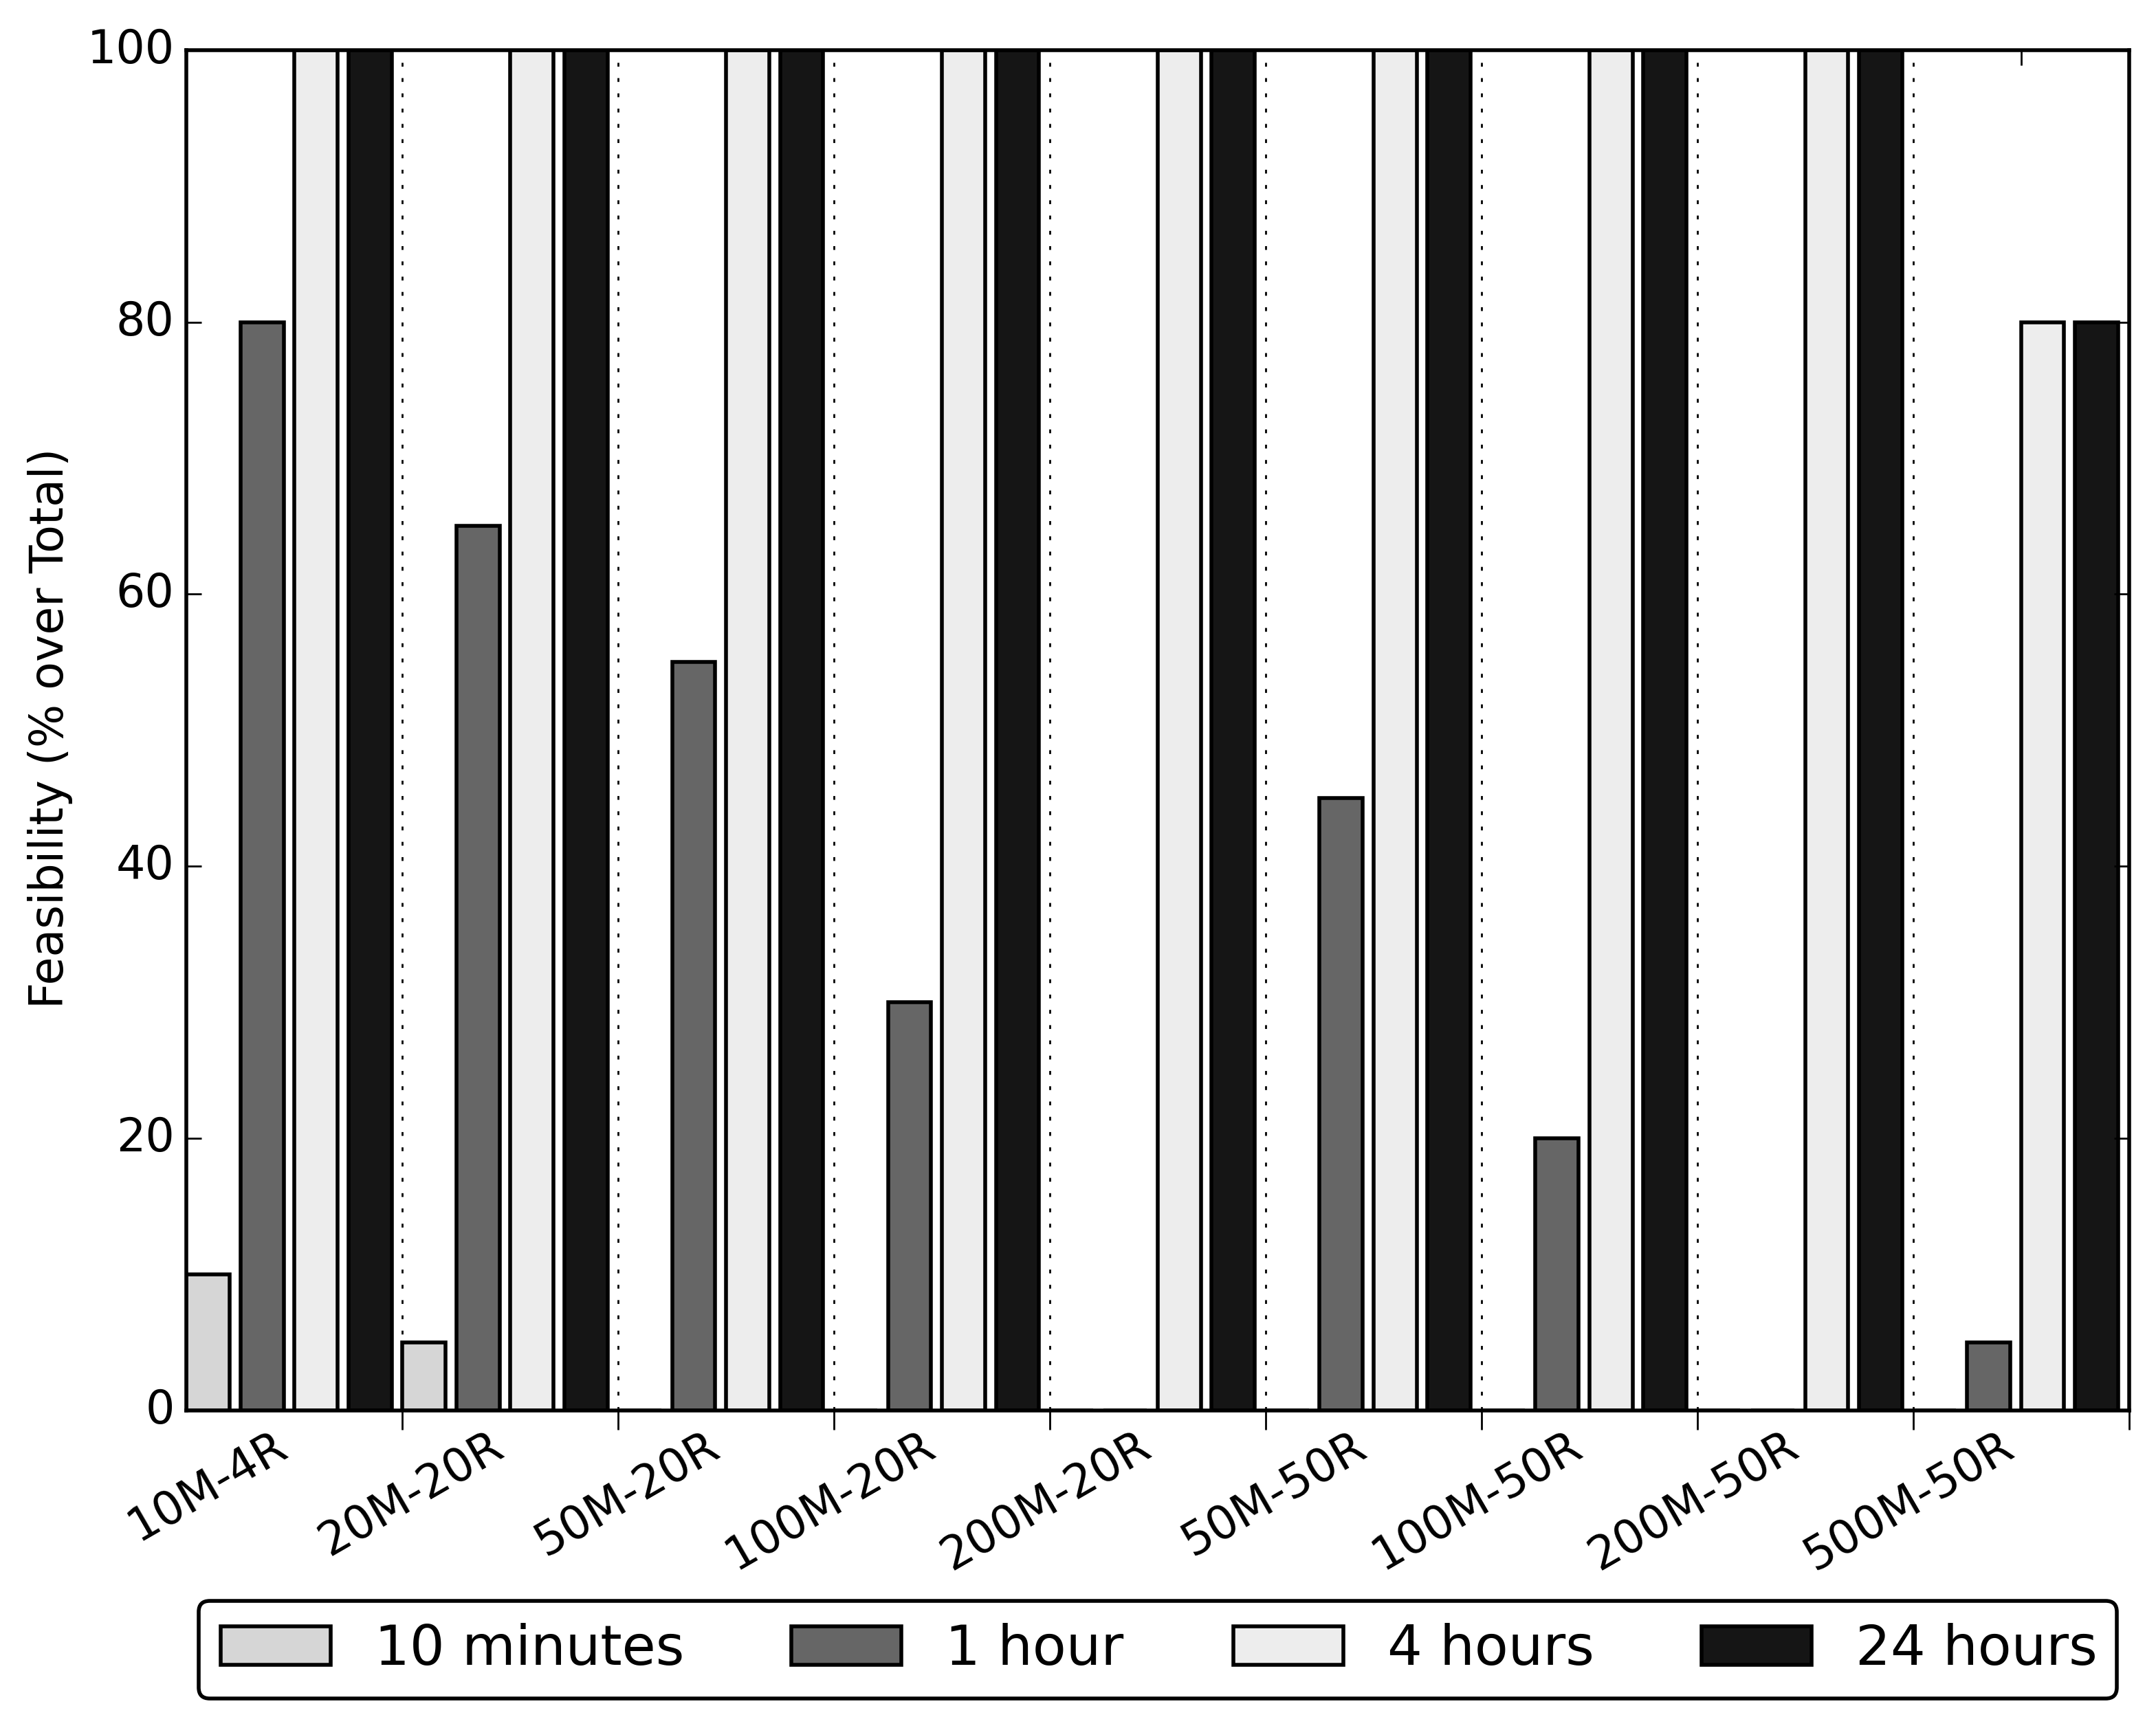
\includegraphics[width=.30\linewidth,keepaspectratio]{figs/feasibility_cvs_oarb_medium_mediumr_mtd.png} &
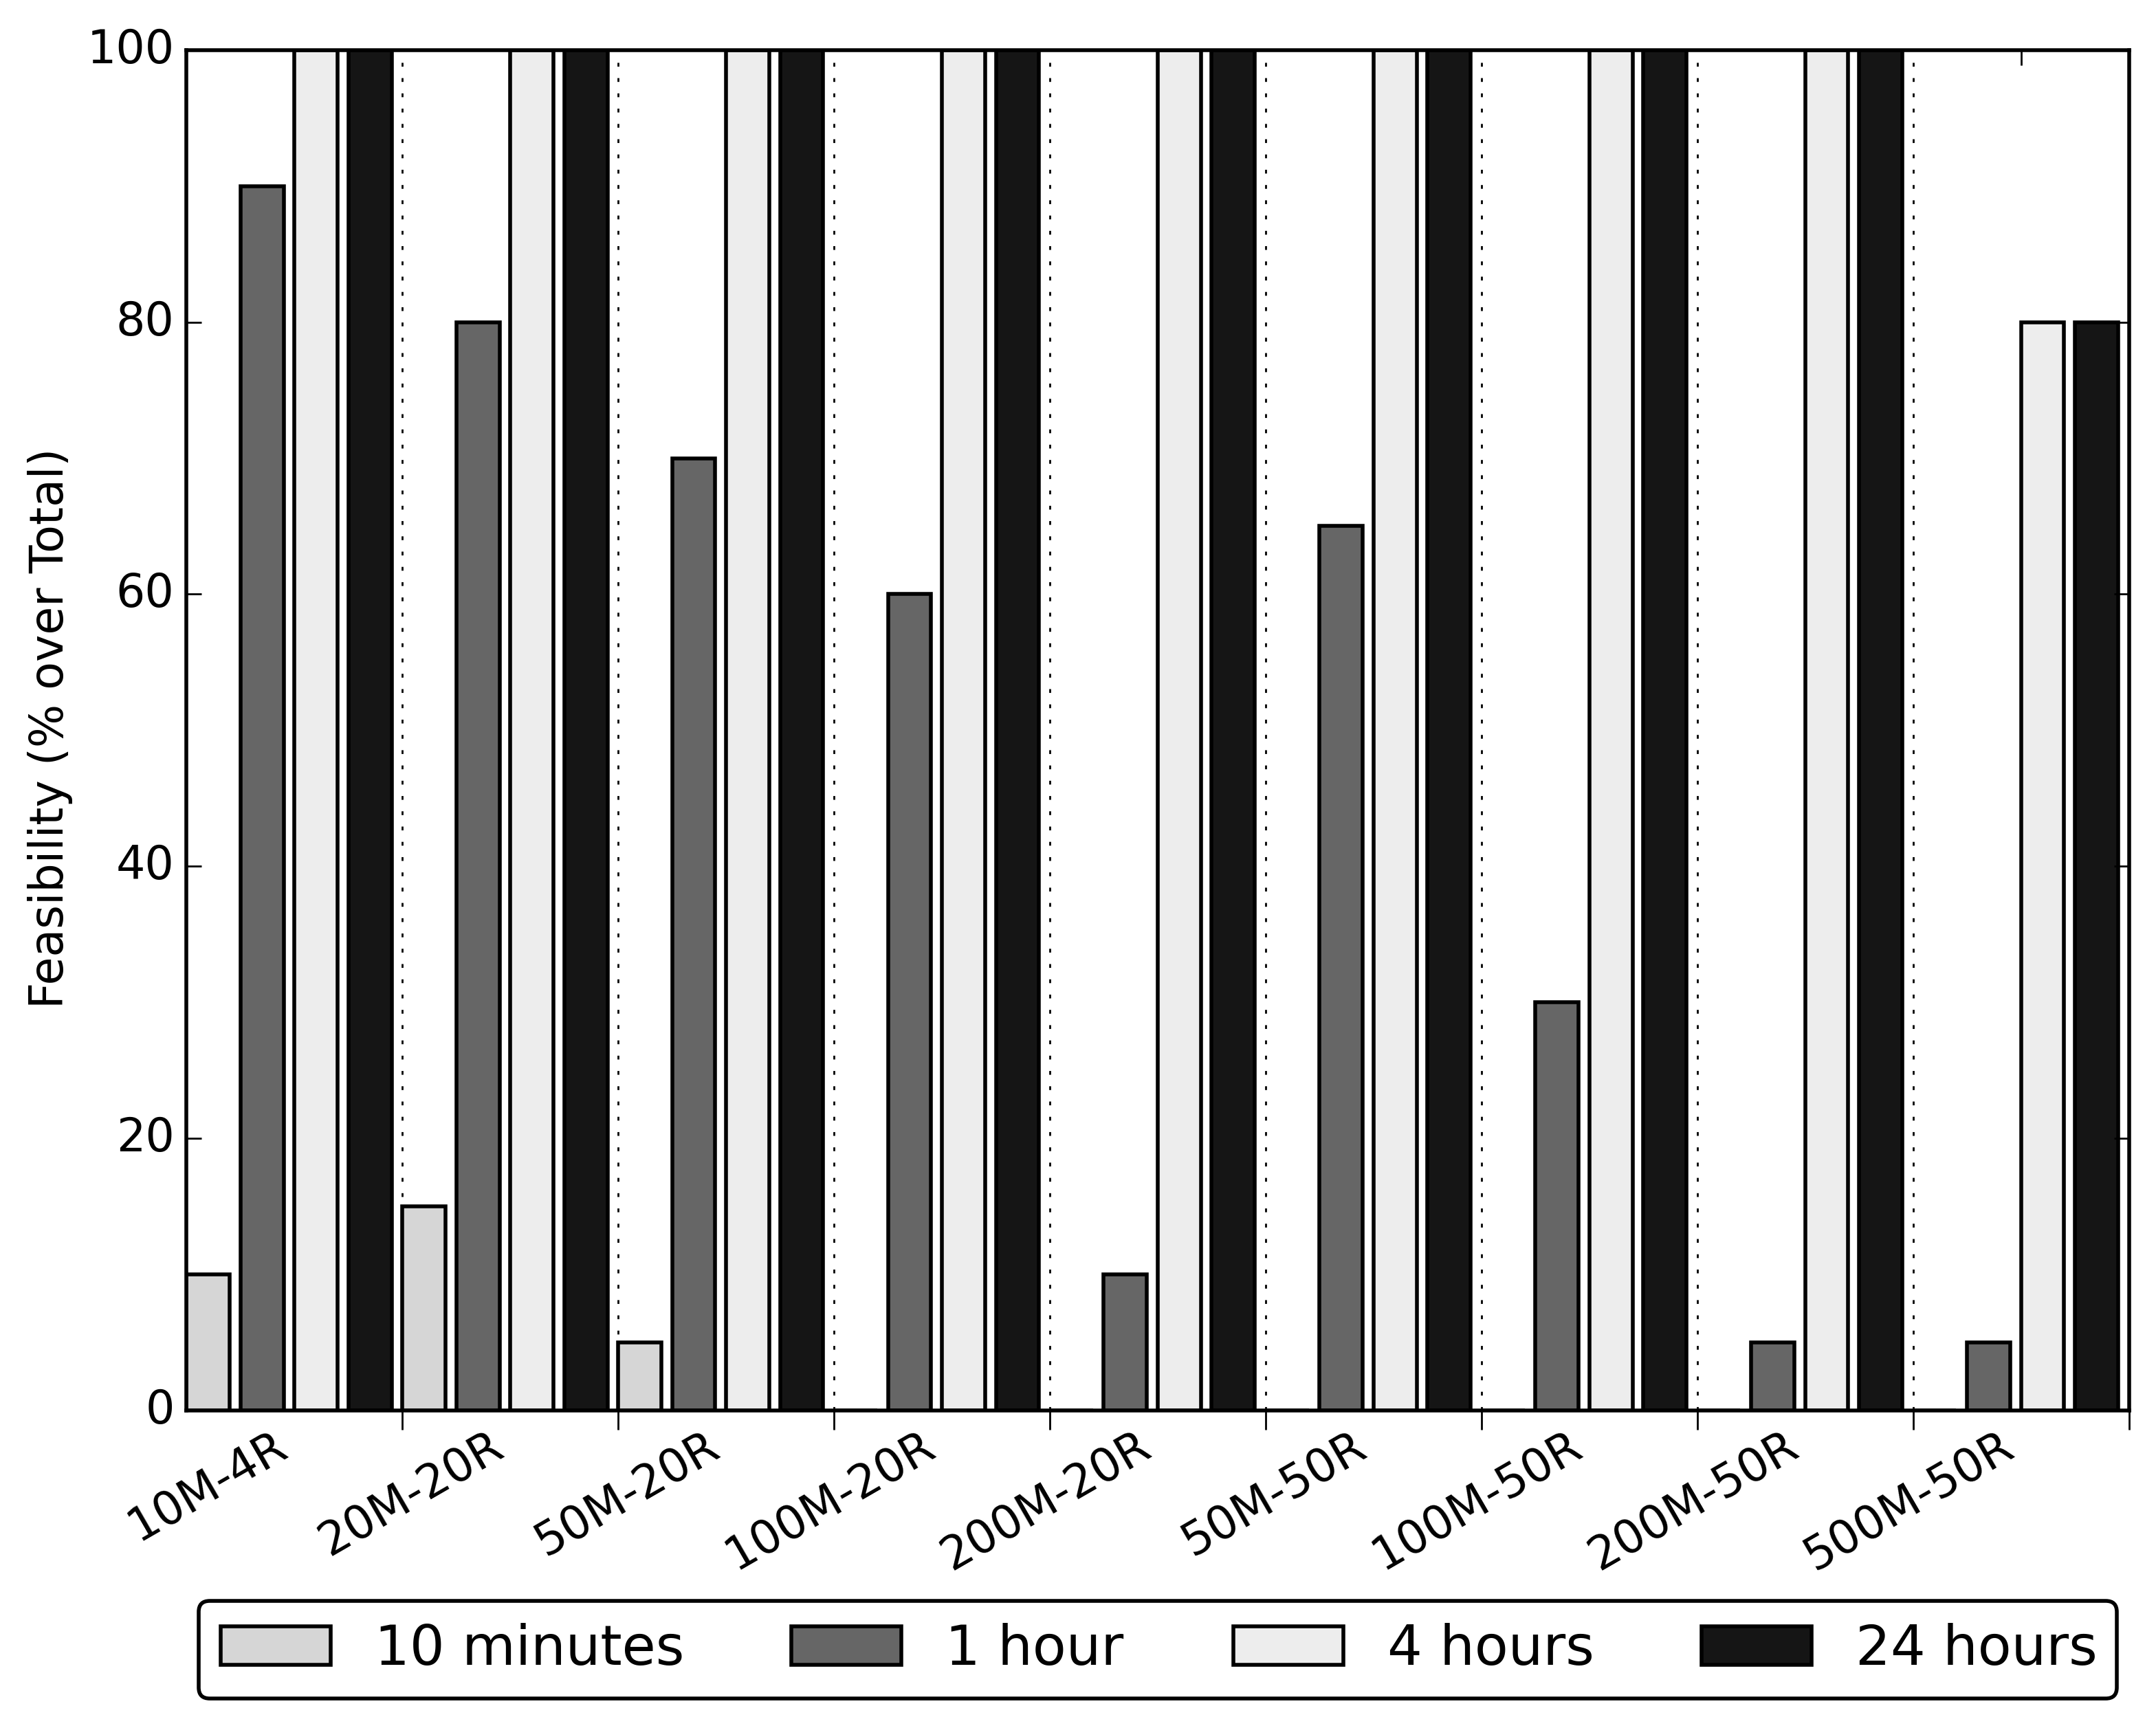
\includegraphics[width=.30\linewidth,keepaspectratio]{figs/feasibility_cvs_oarb_medium_lowr_mtd.png} \\
(a) MDHG & (b) MDMG & (c) MDLG
\end{tabular}
\caption{MTDA approach - solution feasibility (Medium Deviation)}
\label{fig:mtd_mfmr}
\end{figure}


\begin{figure}
\begin{tabular}{ccc}
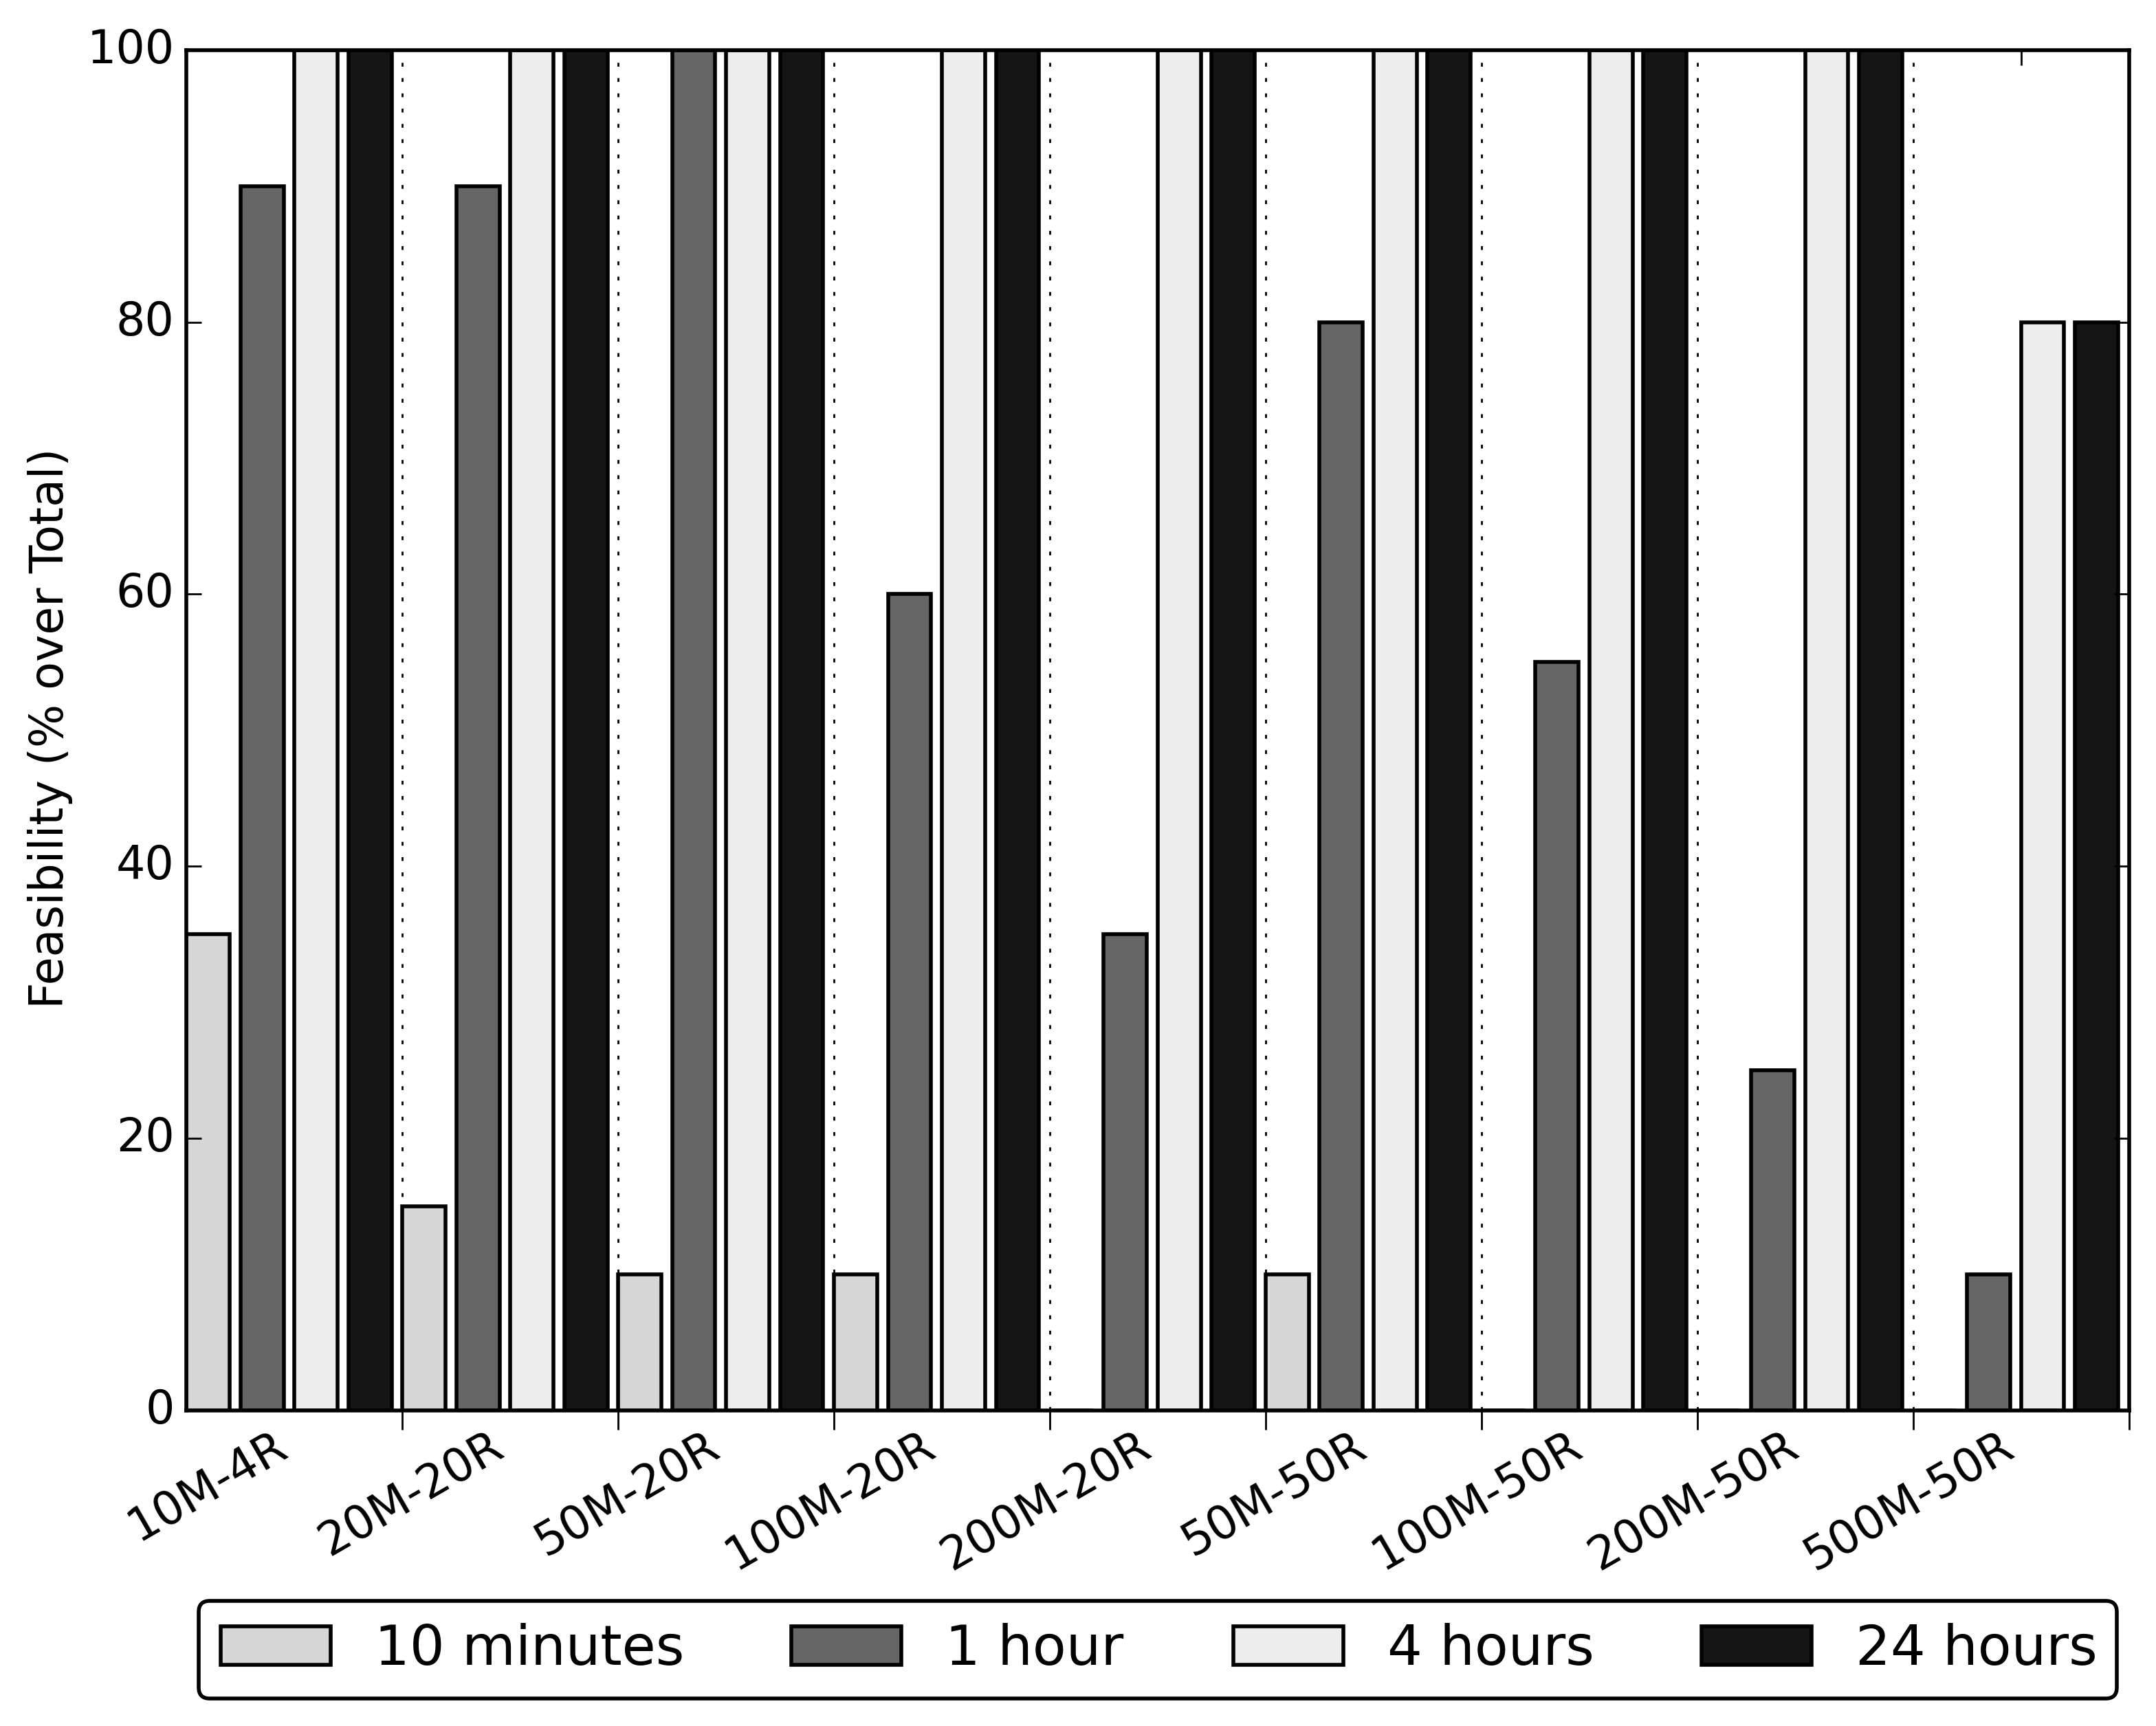
\includegraphics[width=.30\linewidth,keepaspectratio]{figs/feasibility_cvs_oarb_high_highr_mtd.png} &
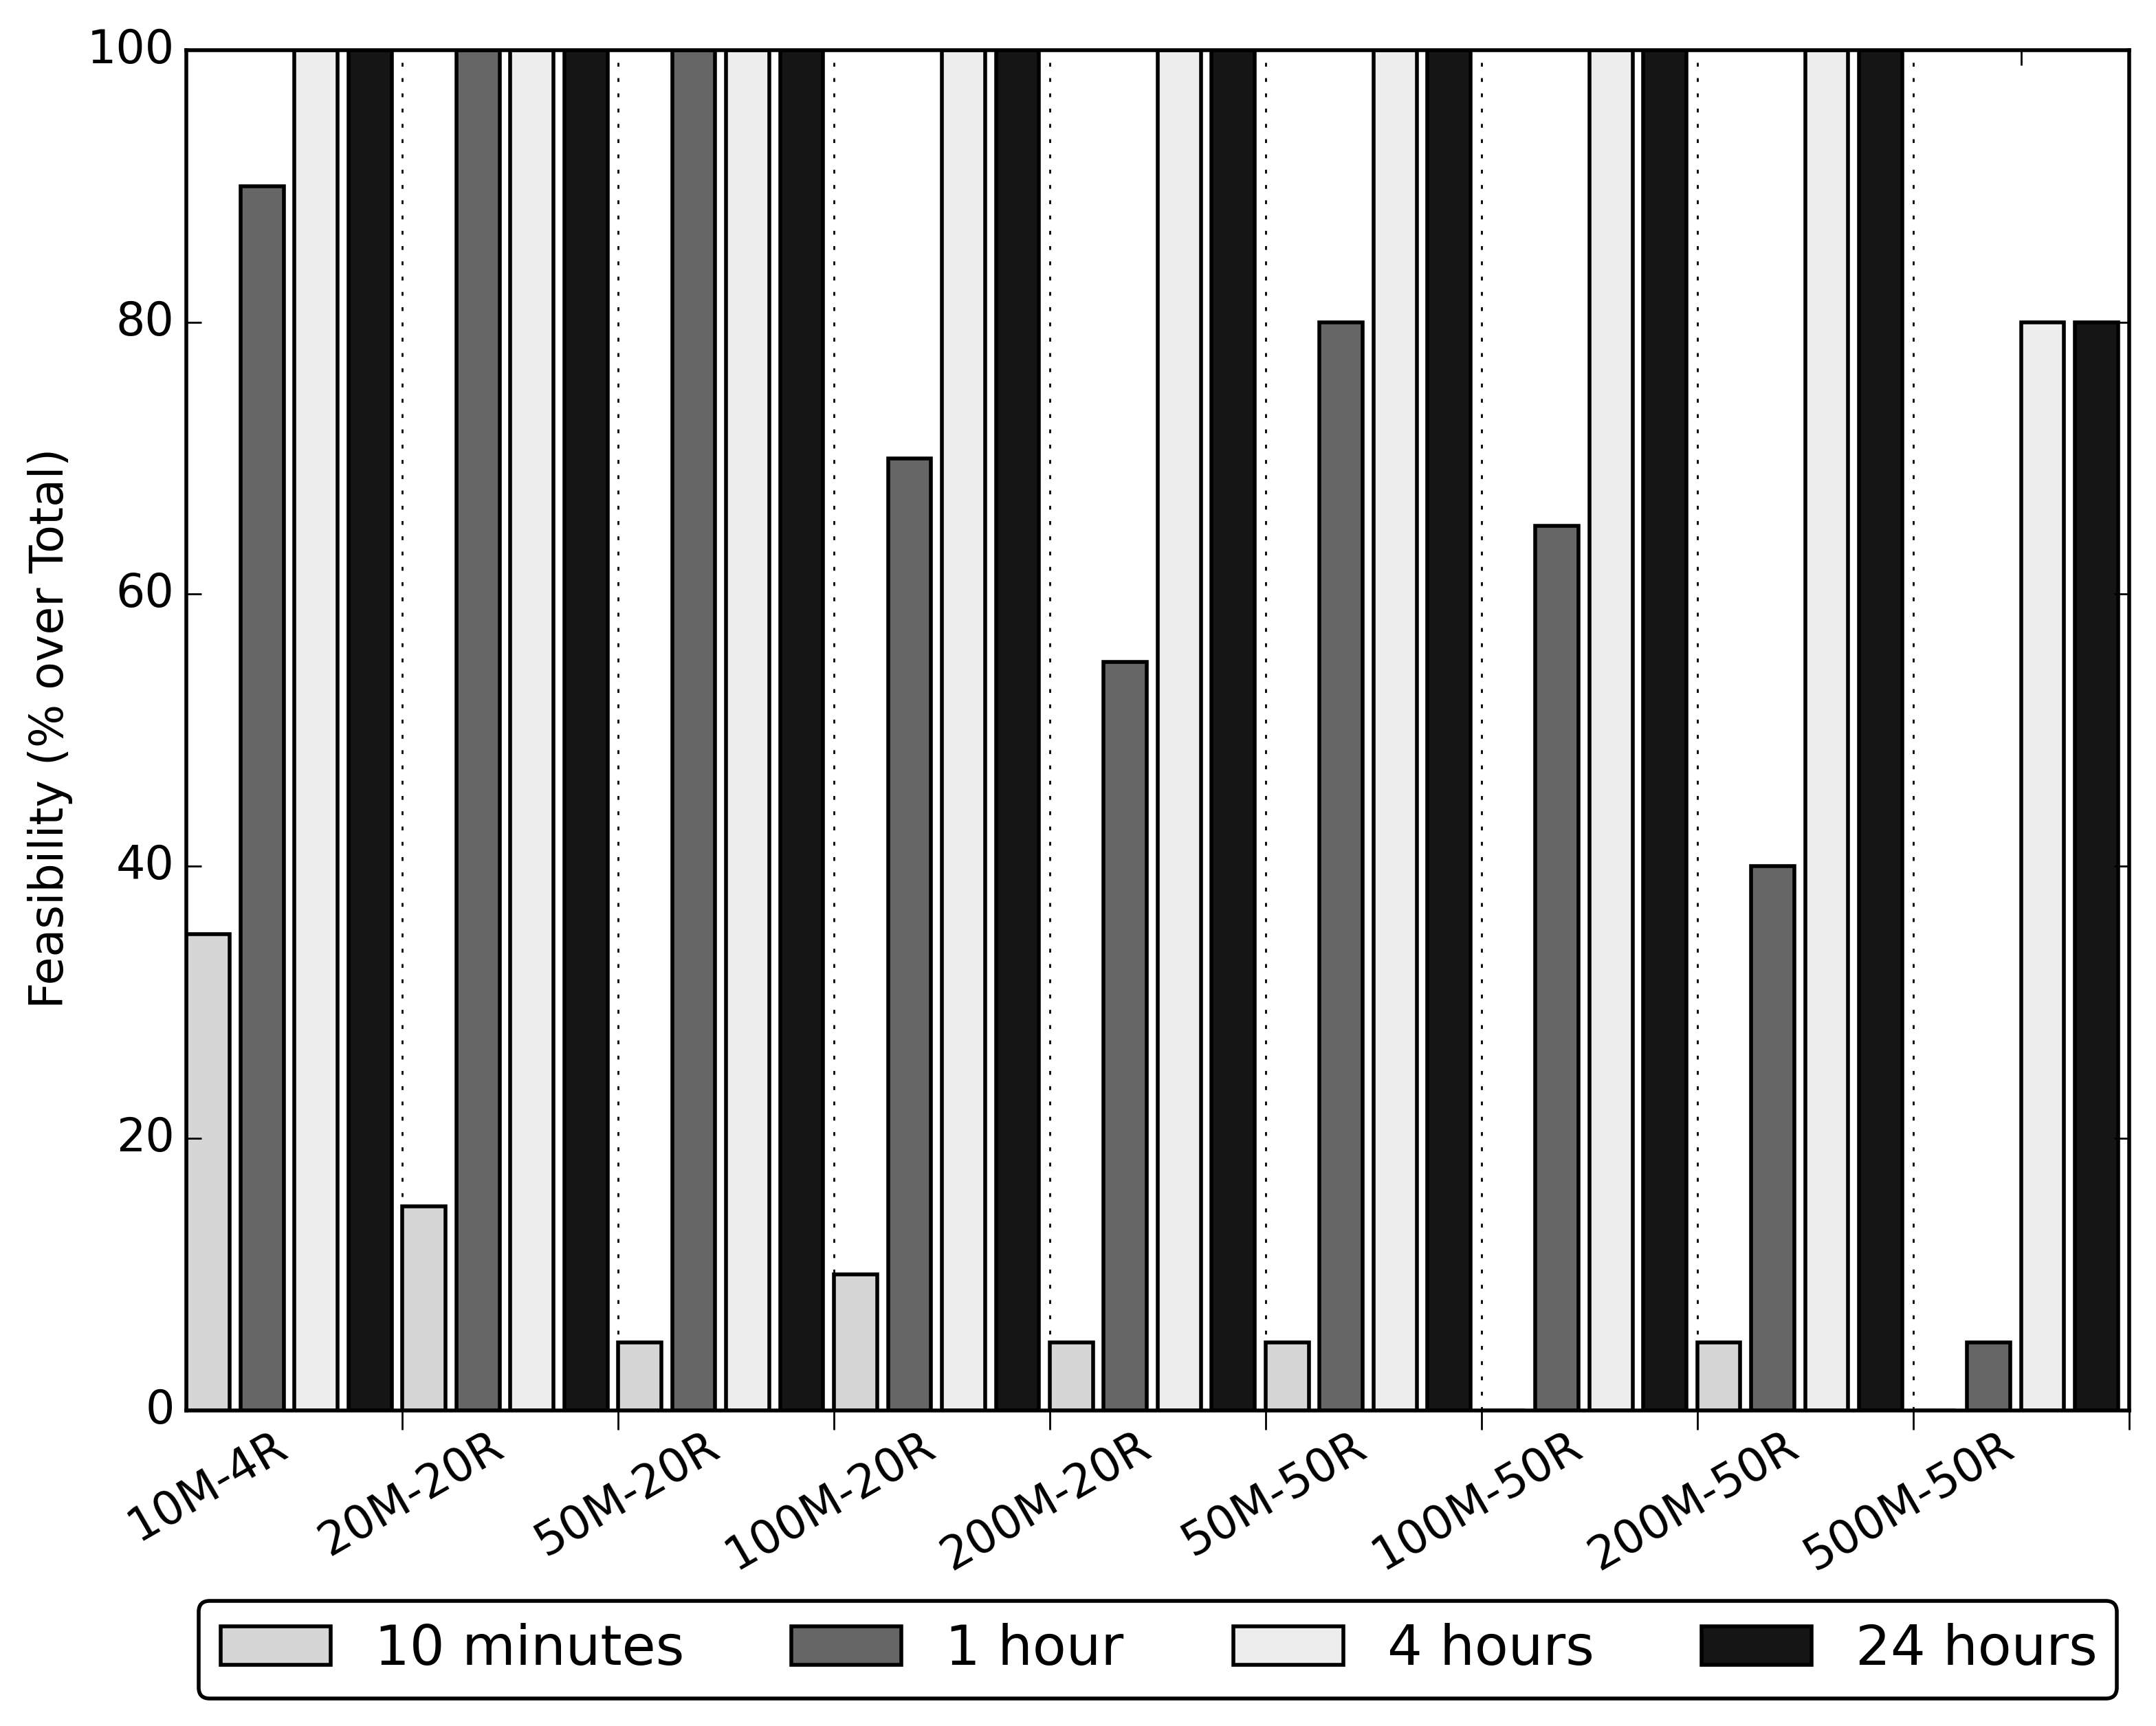
\includegraphics[width=.30\linewidth,keepaspectratio]{figs/feasibility_cvs_oarb_high_mediumr_mtd.png} &
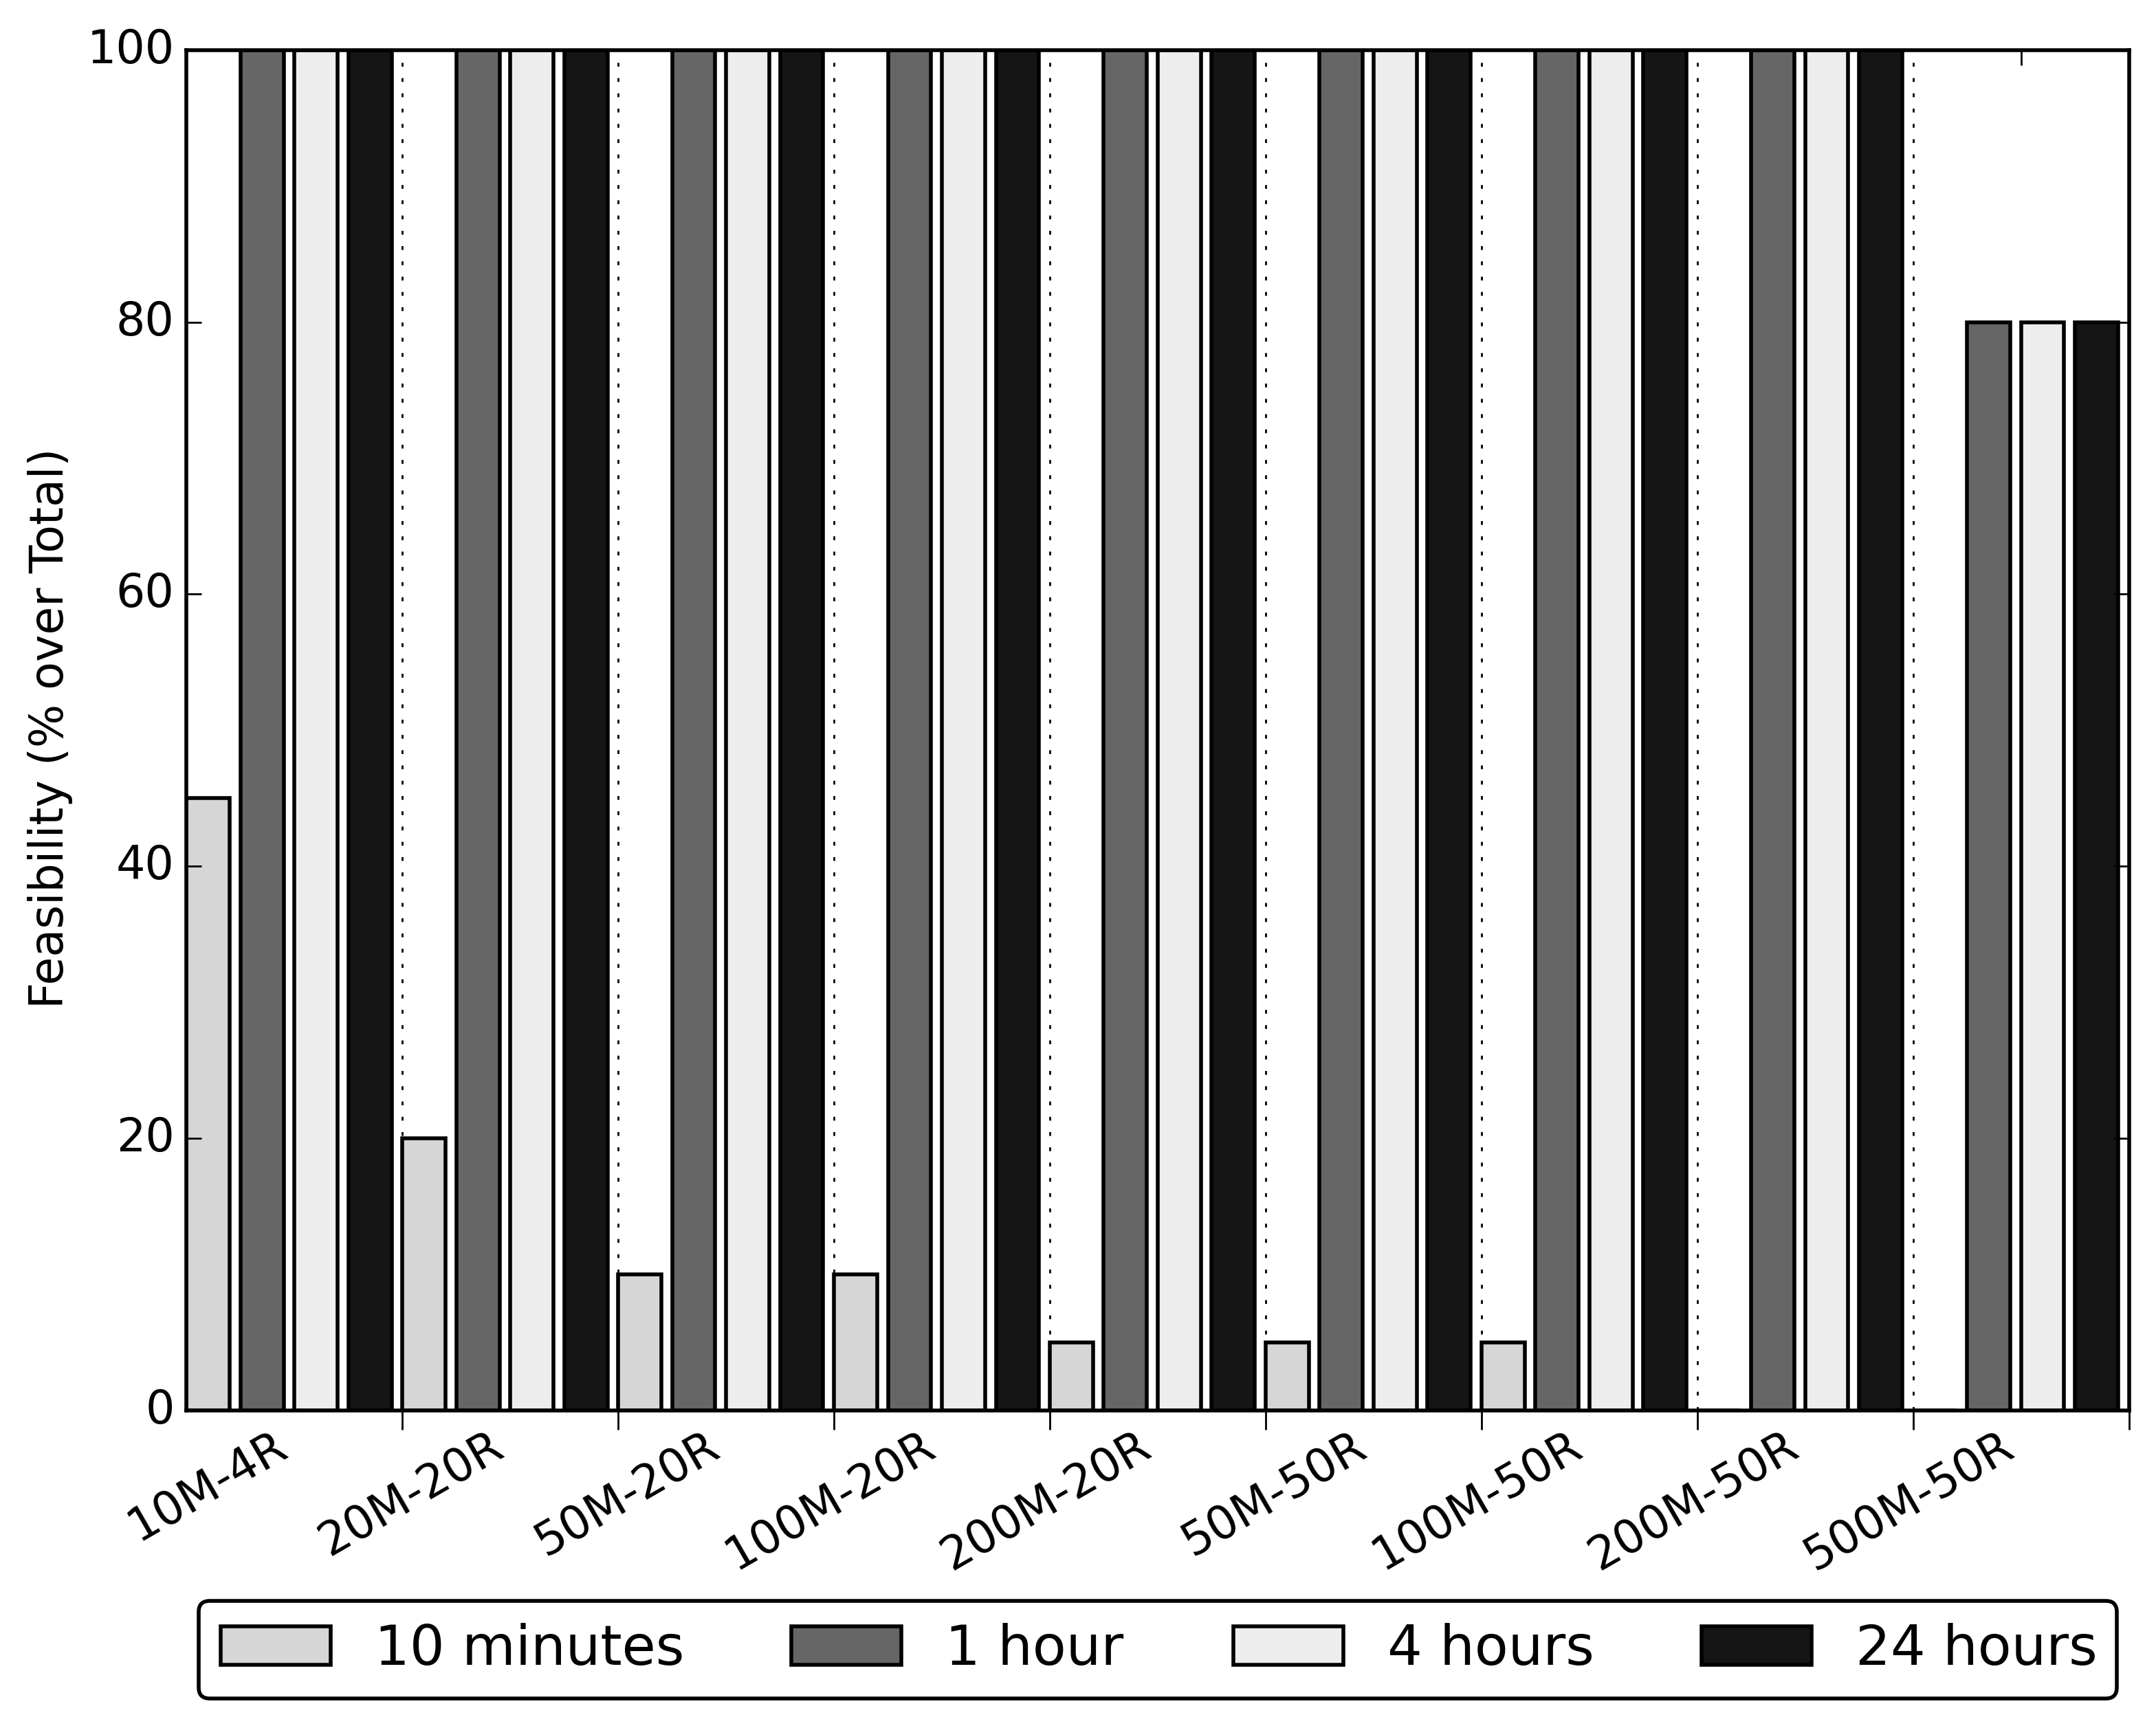
\includegraphics[width=.30\linewidth,keepaspectratio]{figs/feasibility_cvs_oarb_high_lowr_mtd.png} \\
(a) HDHG & (b) HDMG & (c) HDLG
\end{tabular}
\caption{MTDA approach - solution feasibility (High Deviation)}
\label{fig:mtd_mfhr}
\end{figure}






% \subsection{Online vs. Offline Adaptive Control} \label{sec:atc_online}

\section{Related Work}\label{sec:atc_related}

\cite{de1998developing} first proposed the idea of variable indoor temperature standard upon an extensive field experiment conducted worldwide to examine the occupants' perception of thermal comfort. Their statistical results show that occupants were tolerant for a significantly wider range of temperatures, explained by a combination of both behavioral adjustment and psychological adaptation. More recently there have been more work on enabling adaptive thermal comfort control to conserve energy in commercial buildings \citep{egan2010the,chew2015adaptive,klein2012coordinating,ward2010automate,yang2013development}.

\cite{egan2010the,chew2015adaptive,mui2003adaptive} build on \cite{de1998developing}'s adaptive temperature control approach. They focus on designing linear regression models that take outdoor air temperature, occupants' clothing insulation, activity level and indoor velocity into account, and calibrated the temperature setpoints based on these models. Field experiments were conducted in fully air-conditioned buildings in Australia, Malaysia and Hong Kong. They have provided more evidence of the advantage of adaptive thermal comfort control in terms of energy savings. 

\cite{ward2010automate} and \cite{west2014trial} consider occupant feedback in their adaptive control approach. They show that when occupants have some form of control over their local environment, for example operable windows, their subjective view of comfort changes, and they are more willing to accept wider operating conditions than those mandated by traditional comfort models. More research has been conducted to predict comfort setpoints based on historical data input by the occupants, for example, \cite{schumann2010learning} propose methods to learn and predict user comfort preferences.

Inspired by this line of work, we introduce the notion of thermal comfort flexibility into our scheduling model. We incorporate occupants' tolerance level as an input, allowing the scheduler to identify the best location and time slots that optimise energy savings while satisfying occupant thermal comfort. Existing work on energy-aware occupancy scheduling \citep{chai2014minimizing,lim2015hvac,lim2015large,majumdar2016characterising,majumdar2012energy,pan2013minimizing,pan2012thermal} assume fixed comfort temperature setpoints and do not consider adaptive setpoints control. 

The work that is closest to ours is that presented by \cite{ono2012risk}. Their work focuses on generating optimal schedules for resident's daily activities (such as time to leave home and when to go to bed) while controlling the emissivity of dynamic windows to reduce HVAC consumption in a smart home. Their model allows for temperature bound violations, but limits the probability of violation using chance constraints with occupant-specified thresholds. It uniformly distributes a percentage of how much risk can be taken at each time step, and calculates the safety margin (i.e. the temperature violation allowed) based on the allocated risk. The risk allocation for each step is computed using a rule-based approach, independently from the optimisation model and therefore is not optimised. In our work, we assign a cumulative thermal violation allowed for each meeting, and the temperature violation for each step is optimised by the model. We also consider a larger scale of occupancy scheduling in commercial buildings, which is more complex than scheduling activities in a single residential household.
%The safety margin is derived from an inverse CDF of a zero mean gaussian distribution with 0.5$^\circ$C deviation, given the allocated risk. 

Robust optimisation has been used extensively in MPC-based HVAC control as a technique to counter uncertainties caused by varying conditions in buildings. This strategy deals with the associated dynamic variations and constraints by changing the boundary conditions over the receding horizon. Examples of robust MPC control include conditioned air temperature control \citep{huang2009robust}, supply air temperature control \citep{anderson2008mimo}, supply air flow rate control \citep{anderson2008mimo}, zone temperature control \citep{al2004robust,huang2011Model} and damper position control \citep{huang2011Model}. These techniques yield consistent control performance in the presence of disturbances and over different operating conditions, hence are widely explored by the HVAC community. 

To the best our knowledge, we are the first to incorporate discrete scheduling decisions into a robust adaptive temperature control approach in  commercial buildings. We explore the novel idea of allowing occupants to specify some degree of acceptable flexibility in temperature regulation and demonstrate that significant benefits stand to be gained in terms of energy savings and scheduling flexibility. This is appealing because it contributes to the stated goal of improving energy efficiency as well as the implicit goal of designing practical approaches that yield reasonable scheduling solutions under a wide range of conditions. %In this case, online scheduling with last minute scheduling requests. 


\section{Conclusion and Future Work}\label{sec:atc_conclusion}

In this chapter, we extend the joint HVAC control and occpancy scheduling model to enable adaptive temperature control, moving away from the conventional fixed comfort temperature setting. The occupant is allowed to indicate their level of tolerance for the room temperature to deviate from the standard heating and cooling setpoints. We have presented two adaptive control approaches: a maximum temperature deviation-aware (MTDA) method, and an outdoor temperature aware (OATA) method. The first method constrains the occupant thermal discomfort to the maximum temperature deviation allowed over a specified period of time during the activity, whilst the second method limits the temperature deviation based on outdoor temperature. 

We show that thermal comfort flexibility significantly impacts energy consumption. Compared to the existing fixed temperature control,  our MTDA approach achieves an energy saving up to 6\% with low temperature flexibility, with a maximum deviation of $0.5^{\circ}\mathrm{C}$ from the original setpoints, and up to 16\% with high temperature flexibility with a maximum of $2.5^{\circ}\mathrm{C}$ deviation from the standard setpoints. For the OATA approach, the energy savings reach up to 14\% throughout the scheduling horizon. Our results indicate that dynamically adjusting temperature setpoints based on occupants' thermal acceptance level can lead to significant energy reduction. We have also shown that given some thermal comfort flexibility, our model is able to schedule requests arriving 10 minutes prior to the start time, and produces substantially more feasible solutions than the conventional fixed temperature setpoints approach. This is accomplished using a robust optimisation approach, and we demonstrate that solution quality and feasibility improve with temperature flexibility.

One problem in our approach is the selection of the control parameters, that is, the input variables that are used to derive cumulative temperature deviation for both MTDA and OATA approaches. % For eg, in OATA approach, p_m={0.5, 0.75, 0.99} does not show significant difference.
In the future we will develop a parameter-tuning method that automatically generate these inputs for different level of temperature flexibility. These parameters can be optimised inline with the energy savings target for each flexibility level, based on the given temperature deviation allowed and historical data from outdoor temperature and activities duration. 

We are also interested in investigating alternative robust optimisation techniques with the aim of further improving the number of feasible solutions for last minute scheduling requests. This can be achieved by revisiting the connection between robust optimisation and stochastic optimisation.%, for example, by formulating a robust model that allows us to control both the probability and the expected value of constraint violations. We also need further experiments to investigate if our adaptive temperature control approaches carry over to various climate conditions. 


%Robust control design may be the selection of the control parameters, including model uncertainty weights and optimisation criteria weights, which is the major part of the controller design.

% In our experiments, the integration of adaptive temperature control further generates up to 12\% of energy savings when a reasonable thermal comfort flexibility is provided.

% this needs to preserve occupants' thermal comfort 
% create an occupied space that is more in tune with the occupants' thermal acceptance level.
% underpinning the work in this chapter is the expectation that the use of adaptive temperature control forms part of the likely pathway to future zero emission commercial buildings.
